\documentclass[10pt,enlgish,openany,twoside,letterpaper]{book}

%Muestra los márgenes del documento para evitar Warnings
%Para activar la siguiente línea quite el simbolo % 
%\usepackage[showframe]{geometry}

%Usando el paquete BibLaTeX
%Cita normal con \cite[página]{} y cita con paréntesis \parencite[página]{}

% Configuración de BibLaTeX
%\usepackage[backend=biber,style=authoryear,maxcitenames=2,maxbibnames=99,giveninits=true,uniquename=false]{biblatex}
%\addbibresource{biblio.bib}

% Personalizar el formato de las citas y la bibliografía
%\DeclareNameAlias{sortname}{family-given}
%\DeclareDelimFormat{multinamedelim}{\addcomma\space}
%\DeclareDelimFormat{finalnamedelim}{\addcomma\space\&\space}
%\DeclareFieldFormat{titlecase}{\MakeSentenceCase*{#1}}
%\DeclareFieldFormat[article,inbook,incollection,inproceedings,patent,thesis,unpublished]{title}{\titlecase{#1}}
%\DeclareFieldFormat{journaltitlecase}{\titlecase{#1}}
%\DeclareFieldFormat{pages}{#1}
%\DeclareFieldFormat{volume}{\mkbibbold{#1}}
%\renewbibmacro{in:}{}
%\AtEveryBibitem{\clearfield{month}}

\usepackage[english]{babel}
\usepackage[utf8]{inputenc}
% Carácteres especiales
\usepackage{fontenc}
% More advance packages

\usepackage{amssymb,amsbsy,mathrsfs,rotating,float,multirow,upgreek,amsmath,lineno,bm}

\usepackage{listings}
\usepackage{pgfplots}
\usepackage{tikz}
\usepgfplotslibrary{groupplots}
\usepackage{longtable}
\setlength{\LTcapwidth}{6in}
\usepackage[utf8]{inputenc}
\usepackage{epsfig,epic,eepic,threeparttable,amscd,here,lscape,tabularx,graphicx }
\usepackage{booktabs}
\usepackage{tabu,array}
\usepackage{overpic}
\usepackage{microtype}
%%%%%%%%%%%
%\usepackage{newtxtext,newtxmath}

%%%%%%%%%%%
\usepackage{caption}
\usepackage{subcaption}
% Permite ver y configurar los parámetros de la página
\usepackage{layout}
%Hyperref permite ver las secciones del texto
\usepackage[hidelinks]{hyperref}
\usepackage[noabbrev,capitalize]{cleveref}

\usepackage{nomencl}

%% This code creates the groups
% -----------------------------------------
\renewcommand{\nomname}{\sffamily List of Symbols and Abbreviations} 

\usepackage{etoolbox}
\renewcommand\nomgroup[1]{%
  \item[\Large\bfseries
  \ifstrequal{#1}{A}{Number Sets}{%
  \ifstrequal{#1}{B}{Symbols}{%
  \ifstrequal{#1}{C}{Abbreviations}{}}}%
]\vspace{10pt}}
\makenomenclature
% -----------------------------------------

\newcommand{\changes}[1]{\textcolor[rgb]{1.00,0.00,0.00}{#1}}




\providecommand{\var}[1]{{\ensuremath{var}}\{#1\}}
\DeclareMathOperator{\tire}{\negthinspace-\negthinspace}
\DeclareRobustCommand{\legend}[1]{%
	\textcolor{#1}{\rule{1ex}{2ex}}%
}
\newcommand{\lineplot}[1]{
	\textcolor{#1}{\rule{1.5ex}{0.3ex}}%
}

%%%% custom colors
\colorlet{color0}{blue!40!gray}% pearson *
\colorlet{color1}{blue!80!gray} %pearson **
\colorlet{color2}{red!40!gray} %n-pearson*
\colorlet{color3}{red!80!gray}%n-pearson**
\colorlet{color4}{green!40!gray} %plv*
\colorlet{color5}{green!80!gray} 

\definecolor{GII}{RGB}{255,255,107}
\definecolor{GI}{RGB}{72,197,72}
\definecolor{GIII}{RGB}{214, 36, 47}

\definecolor{frontal}{RGB}{141, 211, 199}
\definecolor{frontal_left}{RGB}{255, 237, 111}
\definecolor{frontal_right}{RGB}{255, 255, 179}
\definecolor{central_right}{RGB}{251, 128, 114}
\definecolor{central_left}{RGB}{204, 235, 197}
\definecolor{posterior_right}{RGB}{253, 180, 98}
\definecolor{posterior_left}{RGB}{217, 217, 217}
\definecolor{posterior}{RGB}{179, 222, 105}
\definecolor{crimson2143940}{RGB}{214,39,40}


%%%%
\definecolor{darkorange25512714}{RGB}{255,127,14}
\definecolor{forestgreen4416044}{RGB}{44,160,44}
\definecolor{steelblue31119180}{RGB}{31,119,180}
%%%%

\newcommand{\Objectiveonename}{}
\newcommand{\Objectivetwoname}{}
\newcommand{\Objectivethreename}{}

%% defining objective names
\renewcommand{\Objectiveonename}{Single-trial kernel-based functional connectivity for enhanced feature extraction in EEG-based MI-BCI}
\renewcommand{\Objectivetwoname}{
KCS-FCnet: Kernel Cross-Spectral Functional Connectivity Network for automatic EEG representation in MI-BCI}
\renewcommand{\Objectivethreename}{qualitative and quantitative post-hoc and intrinsic interpretation for MI-BCI models}

%%%


% Create author commands
\newcommand{\studentname}{}
\newcommand{\submissiondate}{}
\newcommand{\academictitle}{}
\newcommand{\resgroupone}{}
%\newcommand{\resgrouptwo}{}
\newcommand{\researchtopic}{}
\newcommand{\thesisname}{}
\newcommand{\director}{}
\newcommand{\codirector}{}
\newcommand{\issuedate}{}
\newcommand{\palabrasclave}{}
\newcommand{\keywords}{}
\newcommand{\schlusselworter}{}
\newcommand{\palavraschave}{}
\newcommand{\sede}{}
\newcommand{\department}{}
\newcommand{\faculty}{}

%Información de la tesis
%Diligenciar aquí los datos para su carga automática donde se requiera en el documento
\renewcommand{\studentname}{Daniel Guillermo García Murillo}
\renewcommand{\thesisname}{Regularized Gaussian Functional Connectivity Network with Post-Hoc Interpretation for Improved EEG-based Motor Imagery-BCI Classification}
\renewcommand{\issuedate}{2024}
\renewcommand{\submissiondate}{01-29-2024}
\renewcommand{\director}{Prof. Dr. Andrés Marino Álvarez Meza}
\renewcommand{\codirector}{Prof. Dr. César Germán Castellanos Domínguez}
\renewcommand{\academictitle}{Doctor en Ingeniería - Ingeniería Automática}
\renewcommand{\resgroupone}{Grupo de control y procesamiento digital de señales (GCPDS) }
%\renewcommand{\resgrouptwo}{}
\renewcommand{\researchtopic}{Inteligencia Artificial}
\renewcommand{\sede}{Manizales} 
\renewcommand{\department}{Departamento de ingeniería y arquitectura}
\renewcommand{\faculty}{Facultad de ingeniería eléctrica, electrónica y computación}


%Palabras clave del documento - Tener presente los Theasurus https://www.thesaurus.com/
%Disponible en 3 idiomas aunque se puede extender a francés o otro idioma

\renewcommand{\palabrasclave}{Use palabras clave que estén en Theasaurus} 
\renewcommand{\keywords}{Use keywords available in Theasaurus}

% Estilo de los encabezados y pies de página
\usepackage{fancyhdr}

\fancyhf{}%
\pagestyle{fancyplain}
\textheight22.5cm \topmargin0cm \textwidth16.5cm \headheight22pt
\oddsidemargin0.5cm \evensidemargin-0.5cm%
\fancypagestyle{plain}{
\fancyhead[RO,LE]{}
\fancyhead[RE,LO]{\small \textbf{\thesisname}}
\fancyfoot[CO,CE]{\thepage}
}
\pagestyle{fancy}
\fancyhf{}%
\renewcommand{\chaptermark}[1]{\markboth{\thechapter.\; #1}{}}
\renewcommand{\sectionmark}[1]{\markright{\thesection.\; #1}{}}
\fancyhead[LO,RE]{\leftmark}
\fancyhead[RO,LE]{\rightmark}
\fancyfoot[CO,CE]{\thepage}
\thispagestyle{fancy}%

\usepackage{titlesec}
% Permite personalizar los títulos de sección y de capítulos
% hang lo deja en el mismo renglón, display lo despliega
% Elimina el "Capitulo" y deja solo el número

\titleformat{\chapter}[hang]
  {\sffamily\Huge\bfseries}{\thechapter}{0.5cm}{\sffamily\Huge}
\titleformat{\section}[hang]{\sffamily\LARGE}{\thesection}{0.5cm}{}
\titleformat{\subsection}[hang]{\sffamily\Large}{\thesubsection}{0.5cm}{}
\titleformat{\subsubsection}[hang]{\sffamily\large}{\thesubsubsection}{0.5cm}{}
\titleformat{\paragraph}[runin]{\sffamily\normalsize}{}{}{\emph}

%Coloca anexo o apéndice en la Tabla de contenido
\usepackage[toc,page]{appendix}

% Configuración de las páginas en twoside-mode
% Permite ver y configurar los parámetros de la página
\setlength{\voffset}{-0.25in}
\setlength{\headwidth}{467pt}
\setlength{\headheight}{22pt}
\setlength{\oddsidemargin}{0pt}
\setlength{\evensidemargin}{0pt}
\setlength{\marginparwidth}{0pt}
\setlength{\marginparsep}{0pt}
\setlength{\parskip}{2em}
\setlength{\footskip}{20pt}
\setlength{\textheight}{650pt}
\setlength{\textwidth}{467pt}
\setlength{\headsep}{5pt}
\setlength{\parindent}{0pt}
\setlength{\baselineskip}{10pt plus 5pt minus 5pt}
\renewcommand{\theequation}{\thechapter-\arabic{equation}}
\renewcommand{\thefigure}{\textbf{\thechapter-\arabic{figure}}}
\renewcommand{\thetable}{\textbf{\thechapter-\arabic{table}}}

%Define la distancia de la primera linea de un parrafo a la margen
\parindent0cm 

%Espacio entre lineas
\renewcommand{\baselinestretch}{1}

%Para rotar texto, objetos y tablas seite.
\usepackage{rotating}

%Permite incluir mecanismos y reacciones químicas
\usetikzlibrary{positioning}
\usetikzlibrary{mindmap}
\usepackage{chemformula}
\usepackage{chemfig}
\usepackage{xcolor}
\usepackage{colortbl}
% use colortbl to avoid using tbale structure from xcolor library, which do not run for this document
% \usepackage[table]{xcolor}

\usetikzlibrary{calc,arrows.meta}% per right to e left to
\tikzset{
myedge/.style={->, -{Latex[#1]}}
}

%Fuente de la presentación Ancizar Sans UNAL
%Para usar este compilado en Overleaf se debe usar el compilador XeLaTeX o LuaLaTeX!!
%Menu -> Compiler -> XeLaTeX o LuaLaTeX
%La siguiente línea debe comentarse si desea compilar con pdfLaTeX
%\RequireXeTeX

% Definición de la fuente Ancizar Sans
\newif\ifxetexorluatex

\ifxetexorluatex
  \usepackage{fontspec}
  \usefonttheme{serif}
  \setmainfont{AncizarSans}[Path=./AncizarSans/,Scale=1,Extension=.otf,UprightFont=*-Regular,BoldFont=*-Bold,ItalicFont=*-Italic,BoldItalicFont=*-BoldItalic]
\else
  % Si se compila con pdfLaTeX, cargar la fuente apropiada aquí
  \usepackage[T1]{fontenc}
\fi
% Metadatos del documento
\AtBeginDocument{%
	\hypersetup{
		pdfborder={0 0 0},
		pdfauthor={\studentname},
		pdfsubject={\thesisname}, 
		pdfcreator={\studentname},
		pdfproducer={\studentname},
	}
}

%Carga el simbolo de grado y el de Angstrom
\newcommand{\angstrom}{\textup{\AA}}
\newcommand{\grad}{$^{\circ}$}

\newtheorem{theorem}{Theorem}[section]
\newtheorem{lemm}{Lemma}[theorem]
\newtheorem{proof}{Proof}[section]
\newtheorem{propo}{Proposition}[theorem]
\newtheorem{definition}{Definition}[section]

%Inicio del documento, no olvide la etiqueta de cierre al final \end{document}
\begin{document}

%% math comands

% custom commands
\providecommand{\ppunto}[2]{\langle#1, #2 \rangle}% producto punto
\providecommand{\promed}[1]{{\mathbb{E}}\left\lbrace #1\right\rbrace}% operador de promedio
\providecommand{\promeddd}[2]{\mathbb{E}_{#1}\!\left\{#2\right\}}% op{\tiny }erador de promedio
\providecommand{\promedd}[2]{\mathds{E}_{#1}\left\{#2\right\}}% operador de promedio
\providecommand{\cov}[2]{{\fam=7 cov}\{#1, #2\}}% operador de covarianza
\providecommand{\gaus}[2]{{\fam=6 N}(#1 #2)} % FDP Gauss
% Kronecker delta function
\providecommand{\Kronecker}[2]{\delta_{K}( #1 , #2 )}
% cardinality
\providecommand{\Cardinality}[1]{| #1 |}



\providecommand{\est}[1]{{\widetilde {#1}}}
\providecommand{\s}[1]{\negthickspace#1\negthickspace}%
\newcolumntype{C}[1]{>{\centering}m{#1}}
\newcommand{\subconj}{\negthinspace\subset\negthinspace }
\newcommand{\en}{\negthinspace\in\negthinspace }
\newcommand{\igual}{\negthinspace=\negthinspace}
\newcommand{\dos}{\negthinspace:\negthinspace}

\newcommand{\Real}{\mathbb{R}}
\newcommand{\Natural}{\mathbb{N}}

\newcommand{\Tr}[1]{Tr \left( #1 \right)}
\newcommand{\diag}[1]{diag \left( #1 \right)}

\newcommand{\func}[1]{\mathcal {#1}}

\newcommand{\ve}[1]{\bm {#1}}
\newcommand{\mat}[1]{\bm {#1}}
%\providecommand{\ve}[1]{{\mathbf {#1}}} %
%\providecommand{\mat}[1]{{\mathbf {#1}}} %

\newcommand{\x}{\negthickspace\times\negthickspace}

%%

%Nombres y formatos de títulos, tablas y figuras
%Use \sffamily para dejar con letra Sans Serif, sin etiqueta queda LaTeX clásico
\renewcommand{\listfigurename}{\sffamily List of Figures}
\renewcommand{\listtablename}{\sffamily List of Tables}
\renewcommand{\contentsname}{\sffamily Content}
\renewcommand{\chaptername}{\sffamily Chapter}
\renewcommand{\tablename}{\scriptsize \centering \textbf{Table}}
\renewcommand{\figurename}{\scriptsize \centering \textbf{Figure}}
\renewcommand{\appendixname}{\sffamily Appendix}

%Cambia el nombre de la sección de referencias
\renewcommand{\bibname}{\sffamily References}

%Páginas de Presentación del documento - No modificar esto se hace automáticamente
{\newpage
\thispagestyle{empty}
\begin{center}
\begin{figure}
\centering

\epsfig{file=Figures/EscudoUN2016,scale=1}%
\end{figure}
\vspace{2.5cm}
\textbf{\Huge \thesisname} \\ 
\vspace{2.5cm}
\textbf{\Large \studentname} \\
\vspace{5.0cm}
\small Universidad Nacional de Colombia \\
\faculty \\
\department \\
\sede, Colombia\\
\issuedate
\newpage 
\thispagestyle{empty}
\vspace{2.5cm}
\textbf{\Huge \thesisname} \\
\vspace{2.5cm}
\textbf{\Large \studentname} \\
\vspace{2.5cm}
\small Tesis presentada como requisito parcial para optar por el título de: \\
{\bfseries \academictitle}\\
\vspace{2.5cm}
Director(a): \\
\director \\
Codirector(a): \\
\codirector \\
\vspace{2.5cm}
Línea de investigación: \\ 
\researchtopic\\
Grupo de investigación: \\
\resgroupone \\
%\resgrouptwo \\
\vspace{2.0cm} 
Universidad Nacional de Colombia \\
\faculty \\
\department \\
\issuedate
\end{center}

% Dedicatorias
\newpage
\thispagestyle{empty}
\begin{flushright}
\begin{minipage}{12.5cm}
\noindent
\\[10em]
%Modificar la cita que se quiere agregar
"Logic will get you from A to B. Imagination will take you everywhere."
\\[3em]
\\ \textit{Albert Einstein}
\\[10em]
%Para anular la adición de una segunda cita anule las siguientes lineas desde acá mediante comentario (%)
"Believe you can, and you are halfway there."
\\[3em]
\\ \textit{Theodore Roosevelt}
%Hasta acá!
\end{minipage}
\end{flushright} 

% Declaracíon de originalidad del texto y del contenido
% No modificar, se hace automáticamente con los comandos ya definidos
\newpage
\chapter*{\sffamily Declaración}
\par Me permito afirmar que he realizado ésta tesis de manera autónoma y con la única ayuda de los medios permitidos y no diferentes a los mencionados el presente texto. Todos los pasajes que se han tomado de manera textual o figurativa de textos publicados y no publicados, los he reconocido en el presente trabajo. Ninguna parte del presente trabajo se ha empleado en ningún otro tipo de tesis. 
\\[1em]
\sede., \submissiondate
\\[6em]
\rule{6cm}{0.5pt}\\
\studentname
}
{\pagestyle{plain} \pagenumbering{roman}
\setlength{\parskip}{1mm}
\chapter*{\sffamily Acknowledgements}
\addcontentsline{toc}{chapter}{Acknowledgements}

Firstly, I extend my gratitude to my supervisor, Andrés Marino Álvarez, and my co-supervisor, Germán Castellanos Domínguez. Their invaluable guidance and support have been indispensable in successfully completing this research. Their contributions have influenced this study and left an indelible impact on my academic journey.

My deepest acknowledgement is extended to my beloved wife who has consistently been a source of strength, providing unwavering support throughout every challenge. Additionally, I wish to express my heartfelt thanks to my dear parents and sister who have persistently stood by me. Their words of wisdom during challenging times and unconditional love have been my pillars of support and stability. Lastly, the most special acknowledgment is reserved for my son, Emanuel, who has been a beacon of joy and hope.

I am particularly grateful to all members of the Signal Processing and Recognition Group (SPRG) at the National University of Colombia in Manizales. A special note of thanks goes to Julian Caicedo and Mateo Tobón whose camaraderie and academic discussions have significantly enriched my experience over these years.

Finally, I recognize that this research would not have been possible without the support given by the projects: “Alianza científica con enfoque comunitario para mitigar brechas de atención y manejo de trastornos mentales y epilepsia en Colombia (ACEMATE).” (Code 111091991908, Hermes Code 56118 ) funded by MINCIENCIAS, and “ Sistema de visión artificial para el monitoreo y seguimiento de efectos analgésicos y anestésicos administrados vía neuroaxial epidural en población obstétrica durante labores de parto para el fortalecimiento de servicios de salud materna del Hospital Universitario de Caldas - SES HUC.” (Hermes Code 57661 ), funded by Universidad Nacional de Colombia.   



\nomenclature[A]{$\Real$}{The set of real numbers}
\nomenclature[A]{$\Natural$}{The set of natural numbers}

\nomenclature[A]{$\mat{X}$}{Matrix}
\nomenclature[A]{$\ve{x}$}{Vector}
\nomenclature[A]{$x$}{Scalar}
\nomenclature[A]{$\func{X}$}{Functional}
\nomenclature[A]{$\Kronecker{\cdot}{\cdot}$}{Kronecker delta function}
\nomenclature[A]{$\Tr{\cdot}$}{Trace operator}
\nomenclature[A]{$\diag{\cdot}$}{Diagonal operator}
\nomenclature[A]{$\Cardinality{\cdot}$}{Set cardinality}
\nomenclature[A]{$\Gamma_{x,x'}$}{Cross-spectral density}
\nomenclature[A]{$\Gamma_{x,x}$}{Power spectral density}
\nomenclature[A]{$\promed{\cdot}$}{Expectation operator}

\nomenclature[B]{$Hz$ }{Hertz}
\nomenclature[B]{$Acc$}{Accuracy performance}
\nomenclature[B]{$s$ }{seconds}
\nomenclature[B]{$mm$ }{Millimeters}
\nomenclature[B]{$N_C$ }{Number of channels/electrodes}
\nomenclature[B]{$N_t$ }{Number of time samples}
\nomenclature[B]{$N_f$ }{Number of filters}
\nomenclature[B]{$N_p$}{Number of features}
\nomenclature[B]{$\mu V$}{Microvolts}
\nomenclature[B]{$mV$}{Milivolts}


\nomenclature[C]{TP}{True positives} 
\nomenclature[C]{FP}{False positives} 
\nomenclature[C]{N}{Number of negative instances} 
\nomenclature[C]{P}{Number of positive instances} 

\nomenclature[C]{TPR}{True positive rate} 
\nomenclature[C]{FPR}{False positive rate}
\nomenclature[C]{EEG}{Electroencephalography}
\nomenclature[C]{MEG}{Magnetoencephalography}
\nomenclature[C]{fMRI}{Functional magnetic resonance imaging}
\nomenclature[C]{CT}{Computed tomography}
\nomenclature[C]{MRI}{Magnetic resonance imaging}
\nomenclature[C]{PET}{Positron emission tomography}
\nomenclature[C]{SPECT}{Single photon emission computed tomography}
\nomenclature[C]{BCI}{Brain computer interface}
\nomenclature[C]{FC}{Functional connectivity}
\nomenclature[C]{SC}{Structural connectivity}
\nomenclature[C]{EC}{Effective connectivity}
\nomenclature[C]{MI}{Motor imagery}
\nomenclature[C]{SMR}{Sensorimotor rhythms}
\nomenclature[C]{ERD}{Event-related desynchronization}
\nomenclature[C]{ERS}{Event-related synchronization}
\nomenclature[C]{CSP}{Common spatial patterns}
\nomenclature[C]{STFT}{Short-time Fourier transform}
\nomenclature[C]{FFT}{Fast Forutier transform}
\nomenclature[C]{CWT}{Continuous Wavelet transform}
\nomenclature[C]{CNN}{Convolutional neural networks}
\nomenclature[C]{RNN}{Recurrent neural networks}
\nomenclature[C]{SBCSP}{Sub-band common spatial pattern}
\nomenclature[C]{CCF}{Cross-Correlation Coefficient}
\nomenclature[C]{PLV}{Phase Lag Value}

\nomenclature[C]{Corr}{Correlation}

\nomenclature[C]{MSC}{Mean square coherence}
\nomenclature[C]{IPC}{Imaginary part of the coherence}
\nomenclature[C]{PC}{Partial coherence}
\nomenclature[C]{PLI}{Phase lag index}

\nomenclature[C]{MI}{Mutual information}
\nomenclature[C]{SL}{Synchronization likelihood}
\nomenclature[C]{Cross-coor}{Cross-correlation}
\nomenclature[C]{GC}{Granger causality}
\nomenclature[C]{TE}{Transfer entropy}
\nomenclature[C]{DTF}{Directed transfer function}
\nomenclature[C]{PDC}{Partial directed coherence}


\nomenclature[C]{CNN}{Convolutional neural networks}
\nomenclature[C]{MLP}{Multilayer perceptron}
\nomenclature[C]{RNN}{Recurrent neural netwrok}
\nomenclature[C]{GNN}{Graph neural network}

\nomenclature[C]{GRU}{Gated recurrent units}
\nomenclature[C]{LSTM}{Long-short-term memory}
\nomenclature[C]{NN}{Neural networks}

\nomenclature[C]{DAE}{Deep autoencoders}
\nomenclature[C]{DRBN}{Deep Restrictive Boltzmann Machine}
\nomenclature[C]{DBN}{Deep believe network}
\nomenclature[C]{GAN}{Generative Adversarial Network}
\nomenclature[C]{VAE}{Variational autoencoder}

\nomenclature[C]{RKHS}{Reproducing Kernel Hilbert Spaces for Machine Learning}

\nomenclature[C]{XAI}{Explainable AI}

\nomenclature[C]{DL}{Deep leanring}

\nomenclature[C]{KCS-FC}{Kernel cross-spectral functional connectivity}
\nomenclature[C]{KCS-FCnet}{Kernel cross-spectral functional connectivity network}
\nomenclature[C]{IRKCS-FCnet}{Interpretable regularized Kernel cross-spectral functional connectivity network}


\nomenclature[C]{DNN}{Deep Neural Networks}

\nomenclature[C]{DCM}{Dynamic causal modeling}
\nomenclature[C]{DTI}{Diffusion tensor imaging}
\nomenclature[C]{TDAH}{Attention-deficit/hyperactivity disorder}
\nomenclature[C]{DSP\&CG)}{Digital Signal Processing and Control Group}

\nomenclature[C]{KCS-FC}{Kernel cross-spectral functional connectivity}
\nomenclature[C]{KCS-FCnet}{Kernel cross-spectral functional connectivity network}
\nomenclature[C]{IRKCS-FC}{Interpretable regularized Kernel cross-spectral functional connectivity network}
\nomenclature[C]{CCA}{Canonical correlation analysis}
\nomenclature[C]{PCA}{Principal component analysis}
\nomenclature[C]{ICA}{Independent component analysis}
\nomenclature[C]{EMD}{Empirical mode decomposition}

\nomenclature[C]{LIME}{Local Interpretable Model-Agnostic Explanations}
\nomenclature[C]{SHAP}{Shapley Additive Explanations}
\nomenclature[C]{TCAV}{ Testing with Concept Activation Vectors}
\nomenclature[C]{xDNN}{Explainable Deep Neural Networks}

\nomenclature[C]{DL}{Deep learning}
\nomenclature[C]{CAM}{Class activation map}

\nomenclature[C]{Grad-CAM}{Gradient Class Activation Map}

\nomenclature[C]{Layer CAM}{Layer Class Activation Maps}

\nomenclature[C]{PSD}{Power Spectral Density}

\nomenclature[C]{RFF}{Random Fourier features}
\nomenclature[C]{KNN}{k-nearest neighbors}
\nomenclature[C]{BP}{Backpropagation}

\nomenclature[C]{DBI MI}{BCI Competition IV dataset IIa}
\nomenclature[C]{DBII ME}{Gamma Motor Execution database}
\nomenclature[C]{DBIII MI}{MI BCI EEG Giga Science database}
\nomenclature[C]{AI}{Artificial Intelligence}




% \nomenclature[A]{}{}
% \nomenclature[A]{}{}
% \nomenclature[A]{}{}
% \nomenclature[A]{}{}
%       $\mathbf{X}$ & Matrix \\
%          $\mathbf{x}$ &Vector\\
%          $x$ & Scalar\\
%          $\mathbf{X}_r \in \mathbb{R}^{C \times T}$ & EEG recording at trial $r$ with $C$ channels and $T$ sample points\\
%          $\mathbf{x}_r^c \in \mathbb{R}^T$ & EEG recording at trial $r$ and channel $c$ \\
%          $y_r \in \mathbb{N}$ & Label at trial $r$\\
%          $\|\cdot\|_q$ & Lq-norm \\
%          $\kappa(\cdot,\cdot;\sigma)$ & Kernel function with bandwidth $\sigma$ \\
%          $\mathscr{F}(\cdot)$ & Fourier transform \\
%          $S_{\cdot,\cdot}(f)$ & Cross-spectral density within frequency domain $f \in \Omega$ \\
%          $R_{\cdot,\cdot}(\tau)$ & Cross-correlation function at time delay $\tau$ \\
%          $\tilde{P}$ & Estimation of a variable $P$ \\
%          $j$ & Imaginary unit\\
%          $|\cdot|$ &Cardinality\\


\printnomenclature[2cm]
\addcontentsline{toc}{chapter}{Symbols and Abbreviations}
\addcontentsline{toc}{section}{Nomenclature}
\addcontentsline{toc}{section}{List of Abbreviations}







% \printnomenclature

% check this page out: 
% https://users.ics.aalto.fi/sami/thesis/node5.html

% https://www.cmor-faculty.rice.edu/~heinken/latex/symbols.pdf

% https://tex.stackexchange.com/questions/469227/how-to-effectively-use-list-of-symbols-for-a-thesis-using-bib-files
% \begin{table}[h]
% \begin{tabular}{ll}
%          $\mathbf{X}$ & Matrix \\
%          $\mathbf{x}$ &Vector\\
%          $x$ & Scalar\\
%          $\mathbf{X}_r \in \mathbb{R}^{C \times T}$ & EEG recording at trial $r$ with $C$ channels and $T$ sample points\\
%          $\mathbf{x}_r^c \in \mathbb{R}^T$ & EEG recording at trial $r$ and channel $c$ \\
%          $y_r \in \mathbb{N}$ & Label at trial $r$\\
%          $\|\cdot\|_q$ & Lq-norm \\
%          $\kappa(\cdot,\cdot;\sigma)$ & Kernel function with bandwidth $\sigma$ \\
%          $\mathscr{F}(\cdot)$ & Fourier transform \\
%          $S_{\cdot,\cdot}(f)$ & Cross-spectral density within frequency domain $f \in \Omega$ \\
%          $R_{\cdot,\cdot}(\tau)$ & Cross-correlation function at time delay $\tau$ \\
%          $\tilde{P}$ & Estimation of a variable $P$ \\
%          $j$ & Imaginary unit\\
%          $|\cdot|$ &Cardinality\\
         
% \end{tabular}
% \end{table}

% An overview of the notation is listed in~\cref{table:simbols}

% \begin{table}[]
% \caption{Symbols and notations}\label{table:simbols}
% \centering
% \begin{tabular}{ll}
% \hline
% \textbf{Symbol} & \textbf{Description}                       \\ \hline
% $N_r \in \mathbb{Z}$   & Number of trials                  \\ \hline
% $N_y \in \mathbb{Z}$   & Number of classes                  \\ \hline
% $N_c \in \mathbb{Z}$   & Number of channels                \\ \hline
% $N_t \in \mathbb{Z}$   & Number of time samples             \\ \hline
% $N_f \in \mathbb{Z}$   & Number of filters              \\ \hline
% $D_m \in \mathbb{Z}$   & Depth multiplier                     \\ \hline
% $D_p \in \left[ 0,1 \right]$   & Dropout rate                        \\ \hline
% $\Delta_t \in \mathbb{Z}$   & Kernel time length                        \\ \hline
% $\textbf{X}_r \in \mathbb{R}^{N_c \times N_t}$   & EEG of a single trial             \\ \hline
% $\textbf{K}_f \in \mathbb{R}^{1 \times \Delta_t}$   & trainable kernel of a convolutional layer             \\ \hline
% $\textbf{D}_r \in \mathbb{R}^{N_c \times N_c}$   & Distance matrix of a single trial \\ \hline
% $\textbf{G}_r \in \mathbb{R}^{N_c \times N_c}$   & Gaussian functional connectivity matrix of a single trial \\ \hline
% $y_r \in \{0,1\}$ & Label of a single trial \\ \hline
% $\textbf{y}_r \in \{0,1\}^{N_y}$ & One-hot label vector of a single trial \\ \hline
% \end{tabular}
% \end{table}

\newpage
\chapter*{\sffamily Resumen}
\addcontentsline{toc}{chapter}{Resumen}%
\par Condiciones como la esclerosis lateral amiotrófica, los derrames cerebrales y las lesiones de la médula espinal pueden causar interrupciones significativas en las vías de comunicación del cerebro, afectando el control muscular voluntario y la interacción con el entorno. Las interfaces cerebro-computadora (BCIs) son sistemas basados en computadoras que se utilizan para abordar estos desafíos; interpretan las señales cerebrales y han sido usadas en aplicaciones médicas, de rehabilitación y de entretenimiento. Particularmente en el campo de BCI, la Imaginación Motora (MI), un paradigma ampliamente investigado, posee un enorme potencial para la recuperación de la funcionalidad motora. La integración de MI-BCIs con terapeutas especializados ha dado resultados positivos en los procesos de rehabilitación sensorial y motora, demostrando ser beneficioso para las personas con trastornos neurológicos. Sin embargo, los sistemas MI-BCI no se limitan a aplicaciones clínicas; también son de gran relevancia en entornos no clínicos como la realidad virtual, los juegos y la adquisición de habilidades motoras.

Usualmente, las señales cerebrales en los sistemas MI-BCI \changes{son} recolectada usando electroencefalografía (EEG) debido a su alta resolución temporal, asequibilidad y portabilidad. Estas características lo convierten en un método viable para capturar eventos de corta duración y patrones de actividad neuronal temporal. No obstante, la decodificación de las señales de EEG es compleja debido a su alta tasa de muestreo y al elevado número de electrodos involucrados, lo que resulta en una cantidad abrumadora de datos. Varias metodologías prometedoras, aprovechando el concepto de sincronización relacionada de eventos (ERS) y desincronización relacionada de eventos (ERD), se han desarrollado para facilitar la extracción de características pertinentes y así decodificar EEG en patrones del area sensoriomotora (SMR). Aunque son importantes, las características de un solo canal tienden a simplificar demasiado los fenómenos generales ya que no consideran las interacciones de las distintas regiones cerebrales. Teniendo en cuenta las activaciones y comunicaciones complejas dentro de varias áreas cerebrales durante la ejecución o la imaginación de tareas motoras sencillas, los enfoques de extracción de características de múltiples canales son más precisos. Por ejemplo, el método de Patrones Espaciales Comunes (CSP) ha demostrado su importancia en MI-BCI, promoviendo la extracción de características altamente discriminativas al maximizar la separabilidad de las características SMR. La conectividad cerebral (BC), un factor clave en estos enfoques, describe las interacciones dentro y entre las regiones cerebrales y se correlaciona con los mecanismos de sincronización dentro de las modulaciones oscilatorias. BC se puede dividir en conectividad estructural/anatómica (SC), conectividad efectiva (EC) y conectividad funcional (FC), cada una con características distintas. SC se centra en conexiones físicas y es independiente del contexto, mientras que EC y FC, adecuados para sistemas MI-BCI basados en EEG, decodifican estados cognitivos de evolución rápida donde FC es particularmente adecuado para aplicaciones de MI-BCI debido a su simplicidad, baja demanda computacional y falta de supuestos previos rígidos.

Esta tesis aborda tres desafíos predominantes en los sistemas MI-BCI basados en FC EEG. En primer lugar, los déficits de rendimiento en las tareas de clasificación de MI son a menudo producto de los altos niveles de ruido presentes en las señales de EEG. En segundo lugar, depender del conocimiento experto para la extracción de características a menudo presenta una barrera. Por último, existe una necesidad de mayor transparencia de dichos modelos. El estudio aporta contribuciones hacia \changes{las FC single-trial} en los sistemas MI-BCI en respuesta a estos desafíos. Esta mejora se logra utilizando un enfoque novedoso basado en la aproximación espectral de kernel cruzado proporcionada por la extensión del teorema de Bochner. Este nuevo estimador de FC de kernel cruzado espectral (KCS) aborda problemas de ruido, conexiones espurias y variabilidad inter-sujeto, mejorando significativamente la precisión. Además, se ha conceptualizado un enfoque end-to-end, KCS-FCnet, para mejorar la representación automática del EEG para MI-BCI. Este enfoque es fundamental para reducir los artefactos e identificar con precisión las conexiones relevantes. Además, ayuda en la extracción de características espectrales, temporales y espaciales del EEG. Reconociendo la necesidad de transparencia del modelo, este estudio propuso una estrategia para mejorar la transparencia e interpretabilidad del modelo, denominada KCS-FCnet regularizada e interpretable (IRKCS-FCnet). Capitalizando el potencial de la regularización, la interpretabilidad del modelo se fortalece minimizando las conexiones no relevantes. Esto se realiza maximizando el potencial de información cruzada utilizando la entropía de Renyi medida en $\alpha=2$, junto con una función de entropía cruzada. Para complementar estas mejoras, se han empleado las estrategias de pesos en la última capa y Layer-CAM para proporcionar interpretabilidad intrínseca y post-hoc, respectivamente. El concepto de caída promedio respalda aún más esta estrategia, mejorando la transparencia y la comprensión del sistema.

Los resultados muestran que el KCS-FC propuesto logra un incremento en el rendimiento que los estimadores clásicos de FC y tiene una precisión competitiva contra estrategias más complejas basadas en FC, alcanzando el segundo lugar en DBI\footnote{BCI2a~\url{http://www.bbci.de/competition/iv/index.html}} con una precisión del $81.92\%$ y el primer lugar con $74.12\%$ en DBIII\footnote{Giga Motor Imagery~\url{http://gigadb.org/dataset/100295}}, ambas tareas de clasificación binaria de MI. Además, el KCS-FCnet muestra un rendimiento $76.4\%$ en DBIII manteniendo la arquitectura con $4245$ parámetros entrenables, lo que lo convierte en el mejor en comparación con los modelos DL comparados. Por último, el IRKCS-FCnet muestra un mejor rendimiento, aumentando $2$ puntos porcentuales para individuos con bajo rendimiento, y muestra una mejor localización e interpretaciones, demostrando que al eliminar el $5\%$ de las características más importantes, la puntuación promedio de caída de precisión cae $22.46$, $5$ puntos porcentuales más alta que la versión sin regularización. Además, se puede ver el patrón contralateral en la interpretación de topoplot para ambas manos, la derecha y la izquierda. Este estudio abre el camino para usar más estimadores de FC dentro de los marcos de DL, y los trabajos futuros pueden extender y mejorar algunos de los problemas existentes, por ejemplo, incluyendo estrategias de medición multivariante y no dependiendo solo de medidas por pares, así como implementar un método de tiempo de retraso para reducir el impacto de los problemas de conducción de volumen. Finalmente, medir las matrices de FC con distancias más apropiadas que tengan en cuenta los enlaces internos entre diferentes canales, como en la geometría de Riemann, podría ayudar a decodificar mejor las señales de MI escondidas en las intrincadas grabaciones de EEG.
\\[2cm]
\textbf{Palabras clave}: Conectividad funcional, Aprendizaje profundo, Métodos de kernel, Entropía de Renyi, Ineficiencia de BCI, Densidad espectral cruzada, Teorema de Bochner.

\newpage 
\chapter*{\sffamily Abstract}
\addcontentsline{toc}{chapter}{Abstract}%
\par Conditions such as amyotrophic lateral sclerosis, brain strokes, and spinal injuries can cause significant disruptions in the brain's communication pathways, affecting voluntary muscle control and interactions with one's environment. Brain-computer interfaces (BCIs) are computer-based systems utilized to address these challenges; they interpret brain signals and have seen extensive applications in medical technology, rehabilitation, and entertainment industries. Particularly in BCI studies, motor imagery (MI), a widely researched paradigm, holds the potential for reviving motor functionality. Integrating MI-BCIs with skilled therapists has yielded positive outcomes in sensory and motor rehabilitation processes, proving to be beneficial for individuals with neurological disorders. Additionally, MI-BCI systems are not limited to clinical applications; they also find relevance in non-clinical settings like virtual reality, gaming, and skill acquisition.

Brain signals in MI-BCI systems are often analyzed using electroencephalography (EEG), which is advantageous due to its high temporal resolution, affordability, and portability. These features make it a viable method for capturing short-evolving events and temporal neuronal activity patterns. Nonetheless, decoding EEG signals is complex due to their high sampling rate and the high number of electrodes involved, which results in an overwhelming amount of data points. Several promising methodologies, leveraging the concept of event-related synchronization (ERS) and event-related desynchronization (ERD), have been developed to ease the extraction of relevant features for decoding EEG into sensorimotor rhythm (SMR) patterns. While noteworthy, single-channel features tend to oversimplify overall phenomena since they need to consider the interactions of different brain regions. Considering the complex activations and communications within multiple brain areas during the execution or imagination of simple motor tasks, multi-channel feature extraction approaches are more accurate. For instance, the Common Spatial Patterns (CSP) method has demonstrated its significance in MI-BCI, promoting the extraction of highly discriminative features by maximizing the separability of SMR features. Brain connectivity (BC), a key determinant in this approach, describes interactions within and between brain regions and correlates to synchronization mechanisms within oscillatory modulations. BC can be divided into structural/anatomical connectivity (SC), effective connectivity (EC), and functional connectivity (FC), each with distinct characteristics. SC focuses on physical connections and is context-independent, while EC and FC, suitable for EEG-based MI-BCI systems, decode fast-evolving cognitive states where FC is particularly suited to MI-BCI applications due to its simplicity, low computational demands, and lack of rigid prior assumptions.

This thesis addresses three prevailing challenges experienced with FC EEG-based MI-BCI systems. Firstly, performance deficits in MI classification tasks are often a result of high noise levels present in EEG signals. Secondly, relying on expert knowledge for feature extraction often presents a barrier. Lastly, there is a necessity for increased transparency within these models. The study delivers key contributions toward a single-trial FC in MI-BCI systems in response to these challenges. This improvement is achieved by utilizing a novel approach grounded on the kernel cross-spectral approximation afforded by extending Bochner's theorem. This new single-trial kernel cross-spectral (KCS) FC estimator tackles noise issues, spurious connections, and inter-subject variability, significantly improving accuracy. Moreover, an end-to-end approach, KCS-FCnet, has been conceptualized to enhance automatic EEG representation for MI-BCI. This approach is pivotal in reducing artifacts and accurately identifying relevant connections. In addition, it assists in the extraction of critical spectral, temporal, and spatial EEG representations. Acknowledging the necessity for model transparency, this study proposed a strategy for improving model transparency and interpretability, named interpretable regularized KCS-FCnet (IRKCS-FCnet). Capitalizing on the potential of regularization, the model's interpretability is strengthened by minimizing nonrelevant connections. This is further made possible by maximizing the cross-information potential using Renyi's entropy measured at $\alpha=2$, alongside a cross-entropy function. To supplement these enhancements, Layer-CAM and last layer weight strategies have been employed to provide both post-hoc and intrinsic interpretability, respectively. The average drop concept further supports these strategies, enhancing the system's transparency and understanding.

The results show that the proposed KCS-FC achieves higher performance accuracy than classical FC estimators and has competitive accuracy against more complex FC-based strategies, reaching the second place in DBI\footnote{BCI2a~\url{http://www.bbci.de/competition/iv/index.html}} with an accuracy of $81.92\%$ and first place with $74.12\%$ in DBIII\footnote{Giga Motor Imager~\url{http://gigadb.org/dataset/100295}}, both binary motor imagery classification tasks. Moreover, the KCS-FCnet shows $76.4\%$ on DBIII while keeping the architecture with $4245$ trainable parameters, making it the highest against the compared DL models. Lastly, the IRKCS-FCnet shows better performance, increasing $2$ percentage points for low-performing individuals, and showed better localization and interpretations, demonstrating that when removing $5\%$ of the most important features, the average accuracy drop score goes to $22.46$, $5$ percentage points higher than the version without the regularization. Furthermore, the contralateral pattern can be seen in the topoplot interpretation for both the right and left hand. This study opens the path for using more FC estimators within DL frameworks, and future work can extend and improve some of the existing issues, for instance, including multivariate measuring strategies and not relying only on pairwise measures, as well as implementing a time-lag method to reduce the impact of volume conduction problems. Finally, measuring FC matrices with more appropriate distances that account for the inner links between different channels, like in the Riemann geometry, could help to better decode MI signals hindered in the intricate EEG recordings.
\\[2cm]
\textbf{Keywords}: Functional connectivity, Deep learning, Kernel methods, Renyi's entropy, BCI inefficiency, cross-spectral density, Bochner's theorem.

%\newpage 
%\chapter*{\sffamily Zusammenfassung}
%\addcontentsline{toc}{chapter}{Zusammenfassung}%
%\par Zusammenfassung texte.
%\par 
%\\[2cm]
%\textbf{Schlüsselwörter:} \schlusselworter
\listoffigures 
\addcontentsline{toc}{chapter}{List of Figures}
\listoftables 
\addcontentsline{toc}{chapter}{List of Tables}
\tableofcontents 
\addcontentsline{toc}{chapter}{Content}
\clearpage
}

{\pagenumbering{arabic}
\setlength{\parskip}{\baselineskip}
%Incluir secciones del documento de aqui en adelante
%Use \include para incluir desde una página nueva e \input para incluir sin salto de página
\chapter{Preliminaries}

\section{Motivation}

Neurological and cognitive conditions such as amyotrophic lateral sclerosis, brain strokes, and spinal injuries can potentially disrupt the communication pathways within the human brain, affecting voluntary muscle control used to communicate with the external environment, such as locked-in syndrome \cite{sisti2022brief, mcfarland2011brain}. To address this, Brain-Computer Interfaces (BCIs) have surged in interest as they are computer-based systems that capture and analyze brain signals, translating them into commands \cite{khan2020review, ramadan2015basics}. 

Motor Imagery (MI), an extensively studied paradigm within BCI research, particularly holds promise in the recovery of motor functionality \cite{bonci2021introductory}. Clinical integrations of MI-BCIs with skilled therapists have proven beneficial in aiding the sensory or motor rehabilitation process, facilitating better environmental interaction for people with neurological disorders \cite{sitaram2017closed, hochberg2012reach,lebedev2006brain}. Beyond clinical applications, MI-BCI systems have seen increased use in non-clinical settings such as virtual reality, gaming, and skill acquisition among healthy subjects \cite{cattan2018recommendations}. Iconic video games such as Pong and Pacman can be played using MI, and studies on healthy subjects show promise in facilitating skills acquisition across various disciplines \cite{ahn2014review, ganin2013p300, johnson2018combined, perdikis2018cybathlon}. 

Nowadays, interest in BCI systems has grown to such a point that before the COVID-19 pandemic, there were more than 150 BCI-based companies distributed in sectors such as automotive, aerospace, medical technology, rehabilitation, robotics, entertainment, marketing, and technology. Besides, the European Commission leads a program called 'The Future of Brain/Neural Computer Interaction: Horizon 2020' to establish a worldwide coordination effort by funding and supporting actions as well as defining a roadmap for future research, taking into account market needs until 2025~\cite{brunner2015bnci}. For instance, the BCI technology market, valued at USD 228.1 million in 2022, is expected to witness substantial growth, with an estimated value of USD 460.1 million by 2029, according to a recent market report \footnote{\url{https://www.marketreportsworld.com/enquiry/request-sample/23789843}}. From a demographic perspective, the value of BCI technology in global socioeconomic development is acknowledged. However, the method for studying this technology varies depending on the specific context of each country, with the USA and China leading in the number of scientific publications, followed by Germany, Japan, and India~\cite{maiseli2023brain}. In this sense, BCI technology development must adhere to the fundamental ideals of humanity, including convenience, ease-of-use, privacy, security, and safety~\cite{willett2021high, matemba2020technology}. 

Neuroimaging techniques are crucial for acquiring brain signals in MI-BCI systems, each playing distinct roles in understanding brain functionality. For instance, Electroencephalography (EEG) and Magnetoencephalography (MEG) capture electrical activity and magnetic fields in the brain, respectively \cite{altaheri2023deep,philip2022non}. Functional Magnetic Resonance Imaging (fMRI) detects changes in blood flow, indicating brain activity \cite{sorger2020real}. Computed Tomography (CT) and Magnetic Resonance Imaging (MRI) provide detailed structural images of the brain, useful in pathology identification \cite{singh2021comprehensive}. Positron Emission Tomography (PET) and Single-Photon Emission Computed Tomography (SPECT) map functional processes in the brain using radioactive substances, highlighting areas with high metabolic activity \cite{veena2020review}. These neuroimaging techniques are summarized in \cref{table:neuroimaging}.

\begin{table}[h]
\centering
\caption{Common neuroimaging techniques principle and working mechanism description}\label{table:neuroimaging}
\scalebox{0.9}{
\begin{tabular}{|l|l|l|}
\hline
\textbf{Technique} & \textbf{Principle} & \textbf{Working Mechanism} \\
\hline
EEG & Records electrical activity & Electrodes on scalp capture voltage fluctuations \\
\hline
MEG & Measures magnetic fields & Superconducting sensors detect magnetic fields \\
\hline
fMRI & Measures blood oxygenation & Detects blood flow changes associated with neural activity \\
\hline
CT & Uses X-rays & X-rays create cross-sectional images \\
\hline
MRI & Uses strong magnetic fields & Protons emit signals for detailed structural images  \\
\hline
PET & Measures emitted gamma rays & Radioactive tracers indicate areas with high metabolic activity\\
\hline
SPECT & Measures emitted gamma rays & Tracers indicate areas with high blood flow\\
\hline
\end{tabular}
}
\end{table}

\cref{fig:neuroimagig} shows the spatial and temporal resolutions and relative cost comparison among the previously mentioned techniques. The color gradient in the figure represents the relative cost of each neuroimaging technique, with green indicating more affordable options and red signifying higher expenses. EEG and MEG are notable for their high temporal resolution, capturing rapid changes in brain activity with millisecond precision \cite{shao2020eeg}. In contrast, fMRI provides excellent spatial resolution, offering detailed insights into brain structures and activity \cite{yuan2021bci}. However, fMRI has a slower temporal resolution than EEG and MEG, making it less suitable for capturing rapid neural dynamics \cite{li2021review}. CT scans, which use X-rays to create cross-sectional images, and MRIs, which use powerful magnetic fields and radio waves, thus avoiding ionizing radiation, both provide detailed anatomical information about the brain's morphology \cite{zhuang2020state}. PET and SPECT focus on functional imaging by detecting radioactive tracers and can reveal metabolic and neurotransmitter activity, but their temporal resolution is relatively lower than EEG and MEG \cite{ramadan2017brain}. While spatial and temporal resolutions are critical factors in selecting the appropriate neuroimaging method, the cost aspect is equally important for decision-making in various research and clinical contexts \cite{rashid2020current}."

\begin{figure}[h!]
    \centering
    \resizebox{0.8\linewidth}{!}{\begin{tikzpicture}[scale=1.2]

% Draw axes
% EEG 0.2
% MEG 0.4
% fMRI 0.8
% CT 0.6
% MRI 0.7
% PET 0.9
% SPECT 0.8

\definecolor{eegcolor}{HTML}{00FF00}
\definecolor{megcolor}{HTML}{66FF33}
\definecolor{fmricolor}{HTML}{FFFF00}
\definecolor{ctcolor}{HTML}{FF9900}
\definecolor{mricolor}{HTML}{FF3300}
\definecolor{petcolor}{HTML}{FF0000}
\definecolor{spectcolor}{HTML}{FF3300}
% X-axis labels
\draw[->] (0,0) -- (10,0) node[right] {Temporal Resolution $(s)$};
\draw (0,0.1) -- (0,-0.1) node[below] {$0$};
\draw (1,0.1) -- (1,-0.1) node[below] {$10^{-3}$};
\draw (2,0.1) -- (2,-0.1) node[below] {$10^{-2}$};
\draw (3,0.1) -- (3,-0.1) node[below] {$0.1$};
\draw (4,0.1) -- (4,-0.1) node[below] {$1$};
\draw (5,0.1) -- (5,-0.1) node[below] {$10$};
\draw (6,0.1) -- (6,-0.1) node[below] {$10^2$};
\draw (7,0.1) -- (7,-0.1) node[below] {$10^3$};

% Y-axis labels
\draw[->] (0,0) -- (0,6.3) node[above] {Spatial Resolution $(mm)$};
\draw (0.1,0) -- (-0.1,0) node[left] {$0$};
\draw (0.1,1) -- (-0.1,1) node[left] {$2$};
\draw (0.1,2) -- (-0.1,2) node[left] {$4$};
\draw (0.1,3) -- (-0.1,3) node[left] {$6$};
\draw (0.1,4) -- (-0.1,4) node[left] {$8$};
\draw (0.1,5) -- (-0.1,5) node[left] {$10$};
\draw (0.1,6) -- (-0.1,6) node[left] {$12$};

\fill[left color=eegcolor!80, right color=petcolor!80] (1,-1) rectangle ++(9,0.2);

\draw (9,-1.1) node[align=center] {Expensive};
\draw (1,-1.1) node[align=center] {Affordable};

% EEG (x,y)
\draw[fill=eegcolor!80] (0.3,4) rectangle (1.8,6) node[pos=.5] {EEG};

% MEG
\draw[fill=megcolor!80] (0.3,2) rectangle (1.8,3.6) node[pos=.5] {MEG};

% fMRI
\draw[fill=fmricolor!80] (3.3,0.6) rectangle (4.6,1.9) node[pos=.5] {fMRI};

% CT
\draw[fill=ctcolor!80] (3.4,0.2) rectangle (4.2,0.55) node[pos=.5] {CT};

% MRI
\draw[fill=mricolor!80] (6.4,0.2) rectangle (7.5,1) node[pos=.5] {MRI};

% PET
\draw[fill=petcolor!80] (5.4,1) rectangle (7,2) node[pos=.5] {PET};

% SPECT
\draw[fill=spectcolor!80] (7,4) rectangle (8,5) node[pos=.5] {SPECT};

\end{tikzpicture}}
    \caption{Comparison of neuroimaging techniques: spatial and temporal resolutions, and relative costs}\label{fig:neuroimagig}
\end{figure}

In particular, MI involves fast-evolving cognitive processes that require superior temporal resolution \cite{varbu2022past}. Therefore, EEG and MEG offer valuable options for capturing short-living events and temporal patterns of neural activity, allowing researchers to observe and analyze brain activity with remarkable temporal precision \cite{alsharif2020neuromarketing}. In addition, due to portability and cost-effectiveness, EEG is the neuroimaging technique most extensively studied by researchers and budget-constrained institutions focusing on MI-BCI applications \cite{janapati2023advances, hosseini2020review, shao2020eeg, khan2020review, lopez2020beyond, ramadan2017brain, fogelson2013functional}. A typical EEG-based MI-BCI system uses a processor unit and an EEG headset equipped with $N_c$ electrodes (channels), varying from $1$ to $256$ \cite{grigorev2021bci, rashid2020current}. These electrodes, attached with an elastic cap, make direct contact with the scalp, recording electrical variations that encode brain activities \cite{varbu2022past}. In addition, some setups may include a monitor for instructing the individual to execute a specific MI task \cite{gu2021eeg}. A visual representation of the setup can be found in \cref{fig:eegsetup}.

\begin{figure}[!ht]
		\centering
		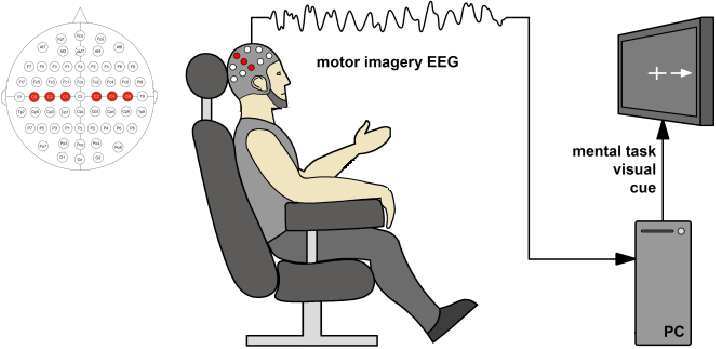
\includegraphics{Figures/preliminaries/EEG-setup.png}
		\caption{Experimental setup for MI-based BCIs. \textbf{{Source}
				:} {Adapted from} \cite{grigorev2021bci}}
		\label{fig:eegsetup}
\end{figure}

Electrical variations recorded by EEG channels are the combination of multiple rhythms that can be used to describe spatially and temporally dynamic patterns of cognitive states within an individual \cite{li2019brain}. The specific neural rhythms that occur in the brain's sensorimotor cortex, an area of the brain involved in planning, controlling, and executing motor functions \cite{leeuwis2021functional}, are known as Sensorimotor Rhythms (SMRs) \cite{altaheri2023deep}. SMRs depend upon individuals and manifest as frequency, shape, and amplitude changes in electrical activity \cite{barios2019synchronization}. In general, most of the cognitive processes implicate six frequency bands: delta [0.5-4]$Hz$, theta [4-8]$Hz$, alpha [8-13]$Hz$, beta [13-30]$Hz$, lower gamma [30-80]$Hz$, and upper gamma [80-150]$Hz$ \cite{khademi2023review, rashid2020current}. Specifically, motor execution and motor imagery actions implicate a frequency range between approximately [4-40] $Hz$ \cite{cattai2021phase}. \cref{tab:freq_bands} describe the most common band types of brain signals according to their frequency ranges.

\begin{table}[h]
    \centering
    \caption{Brain signals classification by frequency range with description}
    \label{tab:freq_bands}
    \begin{tabular}{p{0.15\linewidth}p{0.15\linewidth}p{0.6\linewidth}}
    \hline
      Brain signal  & Frequency range & Description\\
    \hline
      Delta ($\delta$)   & 0.5 to 4 $Hz$ & Slowest brain wave with the highest amplitude, dominant during deep sleep\\
      Theta ($\theta$)  & 4 to 8 $Hz$ & Dominant during deep relaxation and dreaming in light sleep. While normal in children, can be abnormal in awake adults \\
      Alpha ($\alpha$) & 8 to 13 $Hz$ & Dominant in wakeful but relaxed states with closed eyes. \changes{Seen in all ages and can indicate white matter health.}  \\
      Beta ($\beta$) & 13 to 30 $Hz$ & Dominant when alert, concentrated, attentive, and calculating. Typically associated with problem-solving, task engagement, and decision-making  \\
      Lower Gamma ($\gamma_l$)   & 30 to 80 $Hz$ & Active during high-level cognitive tasks \\
      Upper Gamma ($\gamma_u$)   & 80 to 150 $Hz$ & Associated with perception, learning, and language processing \\
      \hline
    \end{tabular}
\end{table}

One of the most important phenomena associated with SMRs is the increase and decrease of oscillatory activity in a particular frequency band during MI tasks, referred to as Event-Related Synchronization (ERS) and Event-Related Desynchronization (ERD) \cite{belwafi2020effective}. ERS and ERD serve as a unique feature of the specific motor action an individual is imagining or executing \cite{zapala2020effects}. This is why several methodologies leverage this critical concept for decoding EEG signals into SMR patterns, aiding in discrimination between MI tasks in EEG-based BCI systems \cite{brusini2021systematic}. 

In general, decoding EEG signals is intricate due to the high sampling rate and number of electrodes, leading to a huge number of data points \cite{singh2021comprehensive}. Therefore, to achieve decent discriminatory capabilities, it is mandatory to perform feature extraction strategies, ensuring a small number of relevant features \cite{ai2019feature}. Feature extraction for MI-BCI systems can be classified into single- or multi-channel approaches.

Single channel perspective relies on the concept of SMRs, and thus, its ultimate goal is to capture oscillatory modulations on specific EEG channels. Time domain strategies collect different temporal information related to a specific MI task, constructing the feature set for a single trial. For instance, statistical features like mean, root mean square, power of the signal, standard deviation variance, skewness, and kurtosis were widely used for MI classification \cite{samuel2017towards, hamedi2014neural}. Other strategies include Hjorth features like activity, mobility, and complexity that indicate the signal power, mean frequency, and change in frequency, respectively \cite{yilmaz2018quasi}. \changes{Simpler strategies like Peak-valley representations, which extract local maximum and local minimum points within a defined timestamp, can also be used to predict MI tasks} \cite{batres2016quaternion}. On the frequency domain side, strategies try to condensate cognitive states within specific frequency bands like in band-power features, that calculates the spectral power in delta, theta, alpha, and beta bands \cite{luo2020motor}; fast Fourier transform, which decomposes EEG signals into its frequency components \cite{rashkov2019natural}; Power Spectral Density (PSD), measuring how the signal power is distributed over frequency \cite{oikonomou2017comparison}. Welch's periodogram, Lomb-Scargle peridiogram, and spectral entropy are methods for extracting or quantifying the PSD of a signal \cite{roy2022comparative, sarraf2017eeg, li2015feature}.

Even though single-channel features can provide useful insights for distinguishing between trials from different MI tasks, it has been shown that oscillatory modulations are not necessarily confined to the sensorimotor cortex \cite{singh2021comprehensive}. Furthermore, the execution or imagination of simple motor tasks activates multiple brain areas that communicate with each other, demonstrating functional integration \cite{ladda2021using}, as opposed to isolated activation of specialized brain regions, known as functional segregation \cite{chiarion2023connectivity}. In brief, by focusing only on single channels, these features may oversimplify the overall phenomenon as they overlook interactions with other regions. Therefore, it is advised to leverage multi-channel feature extraction approaches to provide a more accurate decoding of MI tasks from EEG \cite{leeuwis2021functional}. Among these approaches, the Common Spatial Patterns (CSP) method has been significant in MI-BCI \cite{yang2021multi}. CSP allows the extraction of highly discriminative features by maximizing the separability of SMR features, identifying spatial filters that increase the variance of relevant patterns within one MI process while diminishing the variance of unrelated ones \cite{gaur2021sliding}.

In addition to CSP strategies, Brain Connectivities (BC), which have been used to describe interactions within and between brain regions \cite{ismail2020graph}, can be linked to SMR synchronization mechanisms within EEG recordings \cite{maksimenko2017macroscopic, chiarion2023connectivity}. Key factors of BC include going beyond isolated EEG signals and giving a comprehensive graph visualization that enables researchers to understand brain dynamics between different cognitive states \cite{collazos2023posthoc, grana2023review, tafreshi2019functional, van2014functional, sakkalis2011review}. These factors assist in diagnosing conditions, monitoring progress, and tailoring treatment strategies by tracking how patterns evolve during recovery, therapy, or disease progression \cite{yen2023exploring, lim2021post}. 


\begin{figure}[h]
     \centering
    \begin{subfigure}[b]{.3\linewidth}
        \centering
        \resizebox{1\linewidth}{!}{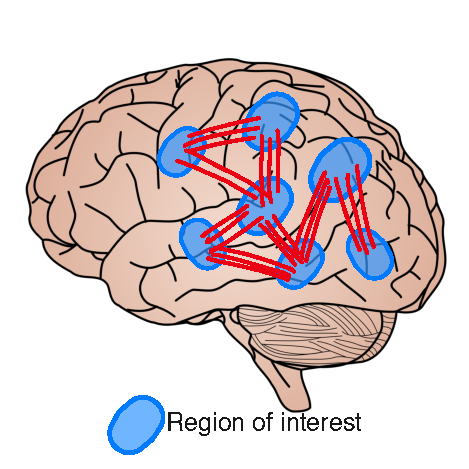
\includegraphics{Figures/preliminaries/SC.pdf}}
        \caption{Structural connectivity\label{fig:SC}}
    \end{subfigure}
    ~
    \begin{subfigure}[b]{.3\linewidth}
        \centering 	\resizebox{1\linewidth}{!}{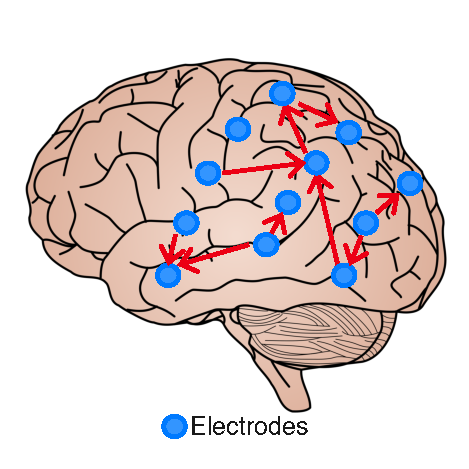
\includegraphics{Figures/preliminaries/EC.pdf}}	
        \caption{Effective connectivity\label{fig:EC}}
    \end{subfigure}
    ~
    \begin{subfigure}[b]{.3\linewidth}
        \centering
        \resizebox{1\linewidth}{!}{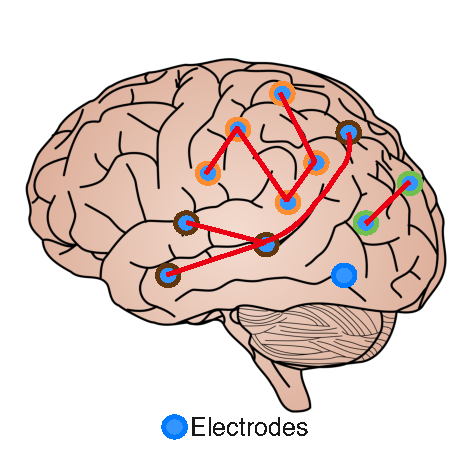
\includegraphics{Figures/preliminaries/FC.pdf}}	
        \caption{Functional connectivity\label{fig:FC}}
    \end{subfigure}
    \caption{Three types of brain connectivities: structural connectivity, effective connectivity, and functional connectivity. Blue circles and blobs represent EEG electrodes and regions of interest, respectively. Circles with different colors represent electrodes with statistical dependencies \label{fig:FC_EC_SC}}
\end{figure}

In general, BC estimates non-directed or directed connections between brain regions and can be divided into three types as depicted in \cref{fig:FC_EC_SC}: Structural/anatomical Connectivity (SC), Effective Connectivity (EC), and Functional Connectivity (FC) \cite{leeuwis2021functional, friston2002functional}. SC, as shown in \cref{fig:SC} focuses on physical connections between different anatomical brain regions, cannot be directly estimated using merely EEG signals and fails to capture short-living events during MI tasks because it is context-independent \cite{thiebaut2020brain, yeh2021mapping}. EC and FC, commonly estimated directly from EEG measures, are suitable for EEG-based MI-BCI systems because they can decode fast-evolving cognitive states \cite{cao2022brain}. According to \cite{friston2013analysing}, EC is always directed and aims to determine how one EEG signal influences another by using parametric models of causal influences as shown in \cref{fig:EC}, while FC can describe directed or non-directed connectives usually via statistical correlation or covariance between EEG signals as shown in \cref{fig:FC}. On one hand, EC requires a deep understanding of the cognitive process to select the most suitable causal model and also demands high computational resources \cite{chiarion2023connectivity, lee2020predicting}. On the other hand, the simplicity of FC, its low computational demands, and the absence of a need for rigid prior assumptions make it particularly well-suited for MI-BCI applications \cite{he2019electrophysiological, hamedi2016electroencephalographic, sakkalis2011review, friston2011functional}.

The Digital Signal Processing and Control Group (DSP\&CG) of Universidad Nacional de Colombia has been working on bio-signal data analysis to propose and develop machine learning methodologies related to automatic systems for the assisted diagnosis of mental conditions \cite{cardenas2017enhanced}, automated analysis of human activity recognition \cite{pulgarin2017relevant}, video analysis based on Multi-Kernel representation \cite{molina2015video}, and biomedical data analysis \cite{hurtado2016identification}. More recently, DSP\&CG works have been focused on extracting relevant patterns from EEG to recognize learning tasks, mainly under the MI paradigm. The used methodologies address dynamic modeling for estimating the spatial relevance of everyday neural activity across subjects \cite{velasquez2020dynamic}, estimation of ERD/S using information theory learning measures \cite{velasquez2020entropy}, enhancement of feature representation based on kernel functional connectivity \cite{garcia2021single}, improving both MI classification and interpretation using convolutional neural networks \cite{collazos2020cnn}. Lastly, BCI performance predictors from deep learning architectures \cite{caicedo2021deep}. Additionally, within \textcolor{black}{the group a variety of research projects are developed}, supported by COLCIENCIAS/MINCIENCIAS, Dirección Nacional de Investigaciones de Manizales (DIMA), and Vicerrectoría de Investigaciones de la Universdiad Nacional de Colombia, such as:

\begin{itemize}
    \item Prototipo de interfaz cerebro-computador de bajo costo para la dectección de patrones relevantes de actividad eléctrica cerebral relacionados con TDAH.
    \item Prototipo de interfaz cerebro-computador multimodal para la dectección de patrones relevantes relacionados con transtornos de impulsividad.
\end{itemize}

From local and general perspectives, integrating MI-BCIs into automatic and semi-automatic rehabilitation systems can provide crucial support for individuals with neurological disorders, aiding in diagnosing conditions, monitoring progress, and tailoring treatment plans. In addition, MI-BCI systems have expanded beyond clinical settings to various applications for healthy subjects, including virtual reality environments, video gaming, and skill acquisition paradigms. EEG's high temporal resolution and affordability make it the most used in MI-BCI clinical and research investigations. Among different feature extraction approaches, multi-channel techniques offer better insights into the actual cognitive state. Specifically, brain connectivity is extensively used in EEG-based MI-BCI systems because it can distinguish between MI tasks; particularly, functional connectivity presents the most suitable strategy for such applications due to their interpretability, low computational demands, and the absence of a need for rigid prior assumptions. The most common issues associated with functional connectivity in EEG-based MI-BCI systems are described in detail in \cref{sec:problem_statement}.
\section{Problem Statement}\label{sec:problem_statement}

As shown in \cref{fig:gen_problem} this thesis will focus its attention on three critical challenges for FC EEG-based MI-BCI. First, despite the valuable insights derived from standard functional connectivity, it faces a performance deficit in MI classification tasks due to the inherently high noise in the EEG signals, issues of volume conduction, and notable inter-subject variability. Second, the heavy reliance on subject matter experts in FC-based feature extraction affects the system's efficiency. This dependence is amplified in scenarios where the same MI cognitive task generates various neural responses in different trials from the same subject, leading to poor and inconsistent predictions. Third, the importance of model transparency to achieve trust among users. With most of the complex models functioning as 'black boxes', predictions are made without clear justifications that can explain why certain decisions are chosen over others, which is crucial for understanding the cognitive processes occurring underneath.

\begin{figure}[!h]
    \centering
    \includegraphics[width=1.0\linewidth]{Figures/problem_statement/general_problem.pdf}
    \caption{Illustration of the three key challenges in FC EEG-based MI-BCI: noise and variability in single trial FC estimators, handcrafted-based subject-specific EEG-based MI-BCI Representation, and the need for model transparency}\label{fig:gen_problem}
\end{figure}


\subsection{Single-Trial FC MI Classification Inefficiency \label{sec:singlefc}}

While standard FC, extracted from various EEG recordings of the same cognitive process (multiple trials), provides invaluable insights for interpreting brain activity patterns, it often struggles to achieve high accuracy in MI classification tasks because single-trial FC estimation only gets a fraction of the data (one trial) \cite{chiarion2023connectivity, rodrigues2020single, billinger2013single}. Since FC quantifies the statistical dependencies between EEG channels, its accuracy estimation is heavily influenced by challenges such as a low signal-to-noise ratio, volume conduction problems, and inter-subject variability \cite{abiri2019comprehensive,bastos2016tutorial}. Therefore, single-trial estimation is an intricate task that usually yields MI classification inefficiency systems \cite{yang2021novel}. 

The inherent noise in signals recorded on the scalp significantly hinders the underlying neural activity, challenging the single-trial estimation from EEG data \cite{si2020predicting, hata2016functional}. Specifically, external or environmental artifacts such as electromagnetic interferences by lighting, AC power lines, and electronic devices; and noise arising from body activities like other cognitive processes, skin resistance fluctuations, electrocardiographic activity (heart functioning), electrooculographic activity (eye movements), electromyographic activity (any muscle movements), and respiration diminish the fidelity of EEG signals~\cite{nentwich2020functional, somers2018generic}. In addition, functional activities recorded using EEG show volume conduction problems even before they can be measured on the scalp's surface, causing several EEG channels to be correlated \cite{qiao2023eeg, varone2021machine}. As a result, many spurious connectivities are induced due to the low signal-to-noise ratio present in EEG signals, impeding competitive performance \cite{bakhshayesh2019detecting}.

Aside from these issues, individual brain activity's intrinsic diversity and complexity also lead to inter-subject variability \cite{wriessnegger2020inter}. The inter-subject variability is not considered a noise per se but an expression of the subjective motor process~\cite{saha2020intra}. For instance, single trial FC-based MI-BCI performance can be negatively affected by the fact that the motor learning process varies over subjects due to intrinsic human kinematic parameters, motivational components, and factors ranging from demographic variables like gender and age to psychological and physiological conditions such as fatigue, relaxation, concentration, and living habits \cite{antonakakis2020inter, huang2023discrepancy}. This is especially evident when different individuals imagine performing the same motor task, leading to varied SMR synchronization patterns that affect FC features~\cite{wriessnegger2020inter, xie2020review}.

Most of the existing single-trial FC estimation methods are based on covariance matrices calculated from the original EEG signal domain and do not account for brain activity's inherent nonlinearity and non-stationarity, inevitably compromising their accuracy \cite{cao2022brain, epmoghaddam2022epileptic, miladinovic2021effect}. Moreover, the high variance in brain activity during task execution adds further difficulties in identifying relevant feature patterns. While improvements in covariance matrix estimation might be achieved through mapping and regularization techniques, selecting an appropriate distance metric to encapsulate variability remains challenging \cite{wang2020diverse,congedo2017fixed}.

In summary, single-trial FC-based MI-BCI systems must enhance the model's accuracy without compromising its interpretability using innovative strategies to effectively manage the complex issues of nonlinearity, non-stationarity, and inter-subject variability. \cref{fig:problem_1} shows a representation of these challenges.

\begin{figure}[!h]
    \centering
    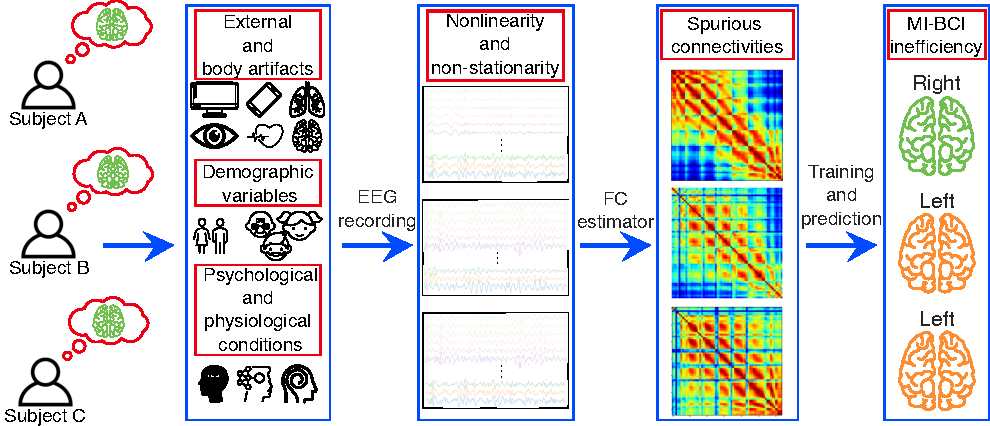
\includegraphics[width=1.0\linewidth]{Figures/problem_statement/problem1_FV.pdf}
    \caption{Single-trial FC-based MI classification inefficiency graphical scheme}\label{fig:problem_1}
\end{figure}


\subsection{Handcrafted-based Subject-Specific EEG-based MI-BCI Representation \label{sec:problem2}}

Despite the substantial progress made in the EEG signals representation in the MI-BCI field, functional connectivity analysis suffers from a high rate of spurious connections due to noise, affecting mainly the accuracy of low-performing individuals \cite{ismail2020graph,wang2020diverse,congedo2017fixed}. This noise within EEG signals significantly contributes to high variability, hindering the underlying neural activity and potentially leading to inaccurate interpretation \cite{caicedo2021deep}. Therefore, EEG signal representation still presents a significant challenge \cite{rashid2020current}.

These challenges arise predominantly from the complexity, degree of sensitivity, and necessity of human experts in EEG representation, such as artifact removal strategies and spatial, temporal, and frequency filtering \cite{chamola2020brain, padfield2019eeg} as graphically illustrated in \cref{fig:problem_2}. For instance, the handcrafted nature of EEG representation leads to high information loss and limits the capacity to detect discriminative correlations among EEG channels, particularly in low-performing individuals \cite{altaheri2023deep}.

While multiple strategies exist for addressing EEG representation issues that can be beneficial in facing MI classification inefficiency, they are often carried out by exhaustive search, limiting the range of artifact removal strategies and spatial, temporal, and spectral filtering selection that can be accomplished \cite{saha2020intra, ismail2020graph, meers2020motor, talukdar2019motor}. In addition, optimizing these steps proves particularly challenging when handling low-performing subjects, even with the insights from subject matter experts \cite{vidaurre2020sensorimotor}.

Despite the considerable advancements in the EEG signal representation within the MI-BCI field, the necessity for human expert intervention in the analysis still poses a significant challenge. In particular, formulating strategies for artifact removal and implementing spatial, temporal, and frequency filters can be exhaustively demanding, especially when dealing with low-performing subjects. The complexity and sensitivity of these strategies often result in a loss of crucial information and limitations in accurately identifying genuine connections between signals, even when guided by subject matter expert knowledge.

\begin{figure}[!h]
    \centering
    \includegraphics[width=1.0\linewidth]{Figures/problem_statement/problem2_VF.pdf}
    \caption{Illustration of challenges in EEG signal representation, including strategies for artifact removal and implementing spatial, temporal, and frequency filters \label{fig:problem_2}}
\end{figure}


\subsection{Lack of Transparency and Interpretability Strategies in MI-BCI \label{sec:problem3}}

The third significant challenge for FC-based MI-BCI systems is model transparency and interpretability, linking back to the core aim of Explainable AI (XAI), which seeks to provide meaningful insights into the reasoning behind model predictions, increasing the confiability, causality, transferability, accuracy, accessibility, and interaction \cite{smuha2019eu}. Integrating various features from different domains into MI-BCI systems poses a unique level of complexity \cite{guillot2019benefits}. For instance, complex models often act like ‘black boxes’, offering outcomes without explanations or justifications \cite{ras2018explanation}, as seen in \cref{fig:problem_3}.

Understanding why models favor specific predictions over others is crucial, not only for predictive efficiency but also in healthcare and medical decision-making scenarios \cite{miotto2018deep}. The interpretation process should highlight the prioritized features during model training and illustrate how these features' interrelationships impact such decisions \cite{zeiler2014visualizing, chakraborty2017interpretability}. As models become more refined, the need for transparency and interpretability amplifies, especially in clinical research where reliance on model recommendations is critical \cite{xiao2018opportunities}.

Moreover, the ongoing debate over the definition of interpretability leads to diverse interpretation methods \cite{fan2021interpretability}. Specifically for FC EEG-based MI-BCI, the challenge lies in creating a quantitative and qualitative interpretability framework that integrates the distinct contributions of each connection to classification across different MI tasks \cite{zuk2020eeg}. Identifying and excluding irrelevant features, especially those generated from noisy functional connectivity patterns, is crucial for model refinement, enhancing its generality, reducing overfitting risks, and expanding the use of MI-BCI in clinical applications like diagnosis, monitoring, and computer-assisted learning \cite{qian2018brain}.

In brief, one of the significant challenges in XAI within MI-BCI systems is ensuring model transparency and interoperability. However, introducing several features from different domains into these systems can be complex. This complexity is exacerbated by models that function like ‘black boxes,’ providing results without explanations. Understanding why specific predictions are favored and how interrelated features influence these decisions is crucial, especially in critical fields like healthcare. In the MI-BCI context, the task lies in forming a quantitative and qualitative framework that can map the individual contributions of each connection within different domains across varying MI tasks for optimizing the model, reducing overfitting risks, and expanding the clinical applications of MI-BCI.

\begin{figure}[!h]
    \centering
    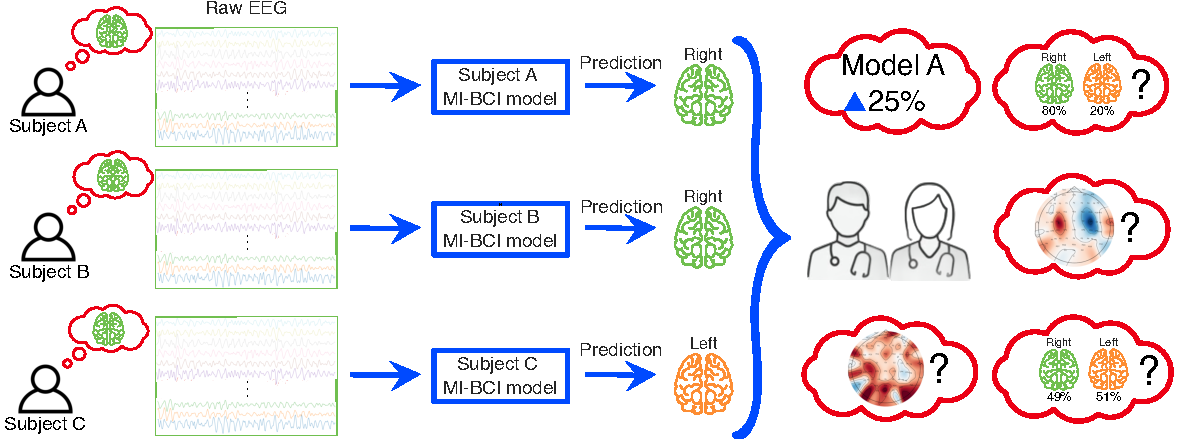
\includegraphics[width=1.0\linewidth]{Figures/problem_statement/problem3_FV.pdf}
    \caption{Transparency and interpretability challenges in MI-BCI models graphical scheme \label{fig:problem_3}}
\end{figure}


\subsection{Research Question}

Given the challenges identified in EEG-based MI-BCI systems, including single-trial FC inefficiency, complexities in EEG representation, and issues of transparency and interpretability in complex models, we propose the following research question:

How can a single-trail FC be developed to manage non-stationary EEG subject-specific representations, handle spurious connectivities, and encode non-linear spatial, temporal, and spectral discriminative and interpretable MI patterns?
\section{State of the Art}

This section presents an overview of the state-of-the-art in the realm of single-trial functional connectivity within EEG-based motor imagery brain-computer interface systems. Our focus is on the cutting-edge approaches designed to tackle the problems described in \cref{sec:problem_statement}, with a subsequent discussion addressing their respective strengths and drawbacks. Initially, we explore single-trial FC feature extraction and estimation. Following this, we discuss end-to-end models that merely depend on the raw EEG data. Lastly, we provide a comprehensive outline of the different interpretability strategies, focusing on deep learning. This overview will allow the reader to comprehend new strategies to clarify the underlying complexities of single-trial FC and its critical role in EEG-based MI-BCI systems.


\subsection{Single-Trial FC in MI-BCI \label{sec:sota1}}

In the context of MI-BCI systems, using FC estimators becomes crucial in decoding the intricate links between different brain parts during MI tasks. These linear and non-linear estimators attempt to measure the statistical dependencies between neurophysiological recordings from different regions, providing crucial insights into brain mechanisms. In addition, FC-based feature extraction techniques play a significant role in effectively translating the nuanced connectivity information into distinguishable patterns related to different MI tasks. When properly extracted and processed, these features enable improved classification and prediction in MI-BCI systems. Over the years, numerous studies have delved into the exploration and enhancement of FC in MI-BCI, leading to significant advancements and understanding. Yet, the field presents challenges and opportunities, particularly considering the complexities and variabilities inherent to brain function and MI processes.


\subsubsection{Functional Connectivity Estimators}

This section offers a review of the most commonly used functional connectivity estimators in the field of EEG-based BCI systems, highlighting their utility and relevance. Given the range of available brain connectivity estimators, selecting an appropriate one is a critical initial step when working with single-trial FC in EEG-based MI-BCI systems. These estimators can generally be broadly categorized based on several factors. First, the domain of interest can be either time or frequency. Second, whether the connectivity is direct or indirect, the former referring to simple zero lag correlation and the latter about the k-lag or cross-correlation. Third, whether the interactions are grounded in a linear or nonlinear formulation. A detailed representation of these categorizations can be found in \cref{fig:sota1_FC}.

\begin{figure}[h]
    \centering
    \resizebox{\linewidth}{!}{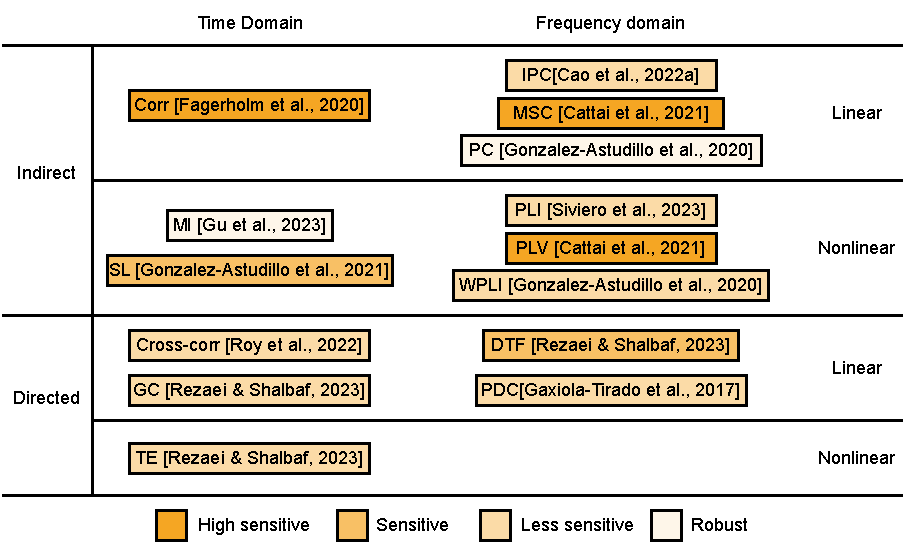
\includegraphics{Figures/state_of_art/sota1_EFC.pdf}}
    \caption{Functional connectivity estimators classified based on direct or indirect, time or frequency domain and linear or nonlinear. The varying shades of orange represent different sensitivities to volume conduction, with lighter shades indicating a higher degree of robustness and solid ones indicating a high level of sensitivity. Abbreviations: Corr, correlation \cite{fagerholm2020dynamic}; MSC, magnitude square coherence \cite{cattai2021phase}; IPC, imaginary part of the coherence  \cite{cao2022brain}; PC, partial coherence \cite{gonzalez2020network}; PLI, phase lag index  \cite{siviero2023functional}; WPLI, weighted phase lag index \cite{gonzalez2020network}; PLV, phase locking value \cite{cattai2021phase}; MI, mutual information \cite{gu2023decoding}; SL, synchronization likelihood \cite{gonzalez2021network}; Cross-corr, cross-correlation \cite{roy2022comparative}; GC, Granger causality \cite{rezaei2023classification}; TE, transfer entropy \cite{rezaei2023classification}; DTF, directed transfer function \cite{rezaei2023classification}; PDC, partial directed coherence\cite{gaxiola2017using} \label{fig:sota1_FC}}
\end{figure}


Linear estimators, due to their straightforward computation and interpretability, have been widely investigated for predicting brain connectivity in MI-BCI systems \cite{gonzalez2020network, van2015opportunities}. The simplest method of estimating linear intercommunication between EEG signals is based on the widely recognized Pearson correlation (Corr) for indirect connectivity and cross-correlation (Cross-corr) for direct connectivity \cite{fagerholm2020dynamic}. It's important to note that Cross-corr is essentially an expanded version of correlation (zero time lag) that considers a k-time lag. As a result, the correlation may not accurately represent linear relationships if there is a delay between specific patterns from two EEG channels \cite{roy2022comparative}. A frequency domain counterpart of correlation is coherence, which is based on the amplitude synchrony of the Power Spectrum Density (PSD) between two EEG signals \cite{cattai2021phase}. Specifically, Magnitude Squared Coherence (MSC), and the Imaginary Part of Coherency (IPC) are two coherence-based FC estimators that are widely used, with the latter being less sensitive to the volume conduction problem \cite{cao2022brain}. While most of the FC estimators rely on the interactions between two signals without removing the influence of other signals, Partial Coherence (PC) and Partial Directed Coherence (PDC) are designed to alleviate spurious connectivities due to common influence from other signals \cite{gonzalez2020network}. Additionally, Directed Transfer Function (DTF) in the frequency domain and Granger Causality (GC) in the time domain employ a multivariate autoregressive model to express one signal as a linear combination of past samples from all the channels \cite{rezaei2023classification}. Nonetheless, these methods are rooted in linear correlations and do not account for the non-linearity inherently present in EEG signals \cite{cao2022effective, mirzaei2021eeg}.

To better understand the nonlinear interactions between EEG channels phase synchronization, usually less affected by volume conduction problems and having direct connection with time delays, becomes a relevant concept \cite{bastos2016tutorial}. Techniques such as the Phase Locking Value (PLV) and Phase Lag Index (PLI) often rely on the phase coupling of oscillatory patterns and are frequently used to measure phase synchronization strength \cite{siviero2023functional}. The Weighted Phase Lag Index (WPLI), created to remove contributions from zero lag, helps to limit misleading connections, but it may miss instantaneous signal interactions \cite{gonzalez2020network}. Information theory techniques have also been effective in revealing nonlinear or complex interactions among EEG signals \cite{jin2021novel}. For example, Mutual Information (MI) and Synchronization Likelihood (SL) can help estimate the likelihood of two EEG channels being correlated \cite{gonzalez2021network}. However, it's important to note that SL can be sensitive to volume conduction problems \cite{chiarion2023connectivity}. On the other hand, Transfer Entropy (TE), used to discover direct connections, stands up well against issues with volume conduction \cite{cao2022brain}. Although nonlinear methods can incorporate more complex FC estimators, they all are prone to problems with spurious connectivities since most noise induced in the EEG leads to nonlinear interactions recorded by different signals that may not reflect genuine relationships \cite{chiarion2023connectivity}.

In brief, linear and nonlinear methods have been developed to extract functional connectivity data from EEG signals. Linear estimators are simple to implement and computationally efficient, but they might not accurately capture complex interactions between EEG channels. Nonlinear methods can address some of these limitations, but they are typically more complex to implement and can be more sensitive to noise in the EEG. While direct connectivity provides information about the direction of information flow between two channels, indirect connectivity only measures the strength of the relationship \cite{gonzalez2020network}. Both direct and indirect connectivity have been shown to achieve similar performance in EEG-based MI-BCI systems, with indirect connectivity being less sensitive to the volume conduction problem \cite{cao2022effective}.

\subsubsection{Feature Extraction from FC}

In conjunction with the selection of single-trial FC estimators, feature extraction techniques are vital for decoding connectivity information, ensuring decent discriminatory capacities between MI tasks \cite{ai2019feature}. Broadly, these techniques can be divided into four primary approaches as shown in \cref{fig:sota1_FE}: CSP which finds linear spatial filters that enhance class discriminability; vector representations that leverage the symmetry of indirect FC to extract the upper triangular values from the adjacency matrix; topological representations that depict FC as brain activation topoplots; and approaches using Riemannian geometry that leverage the manifold of symmetric positive definite matrices.

\begin{figure}[h!]
    \centering
    \resizebox{1.1\linewidth}{!}{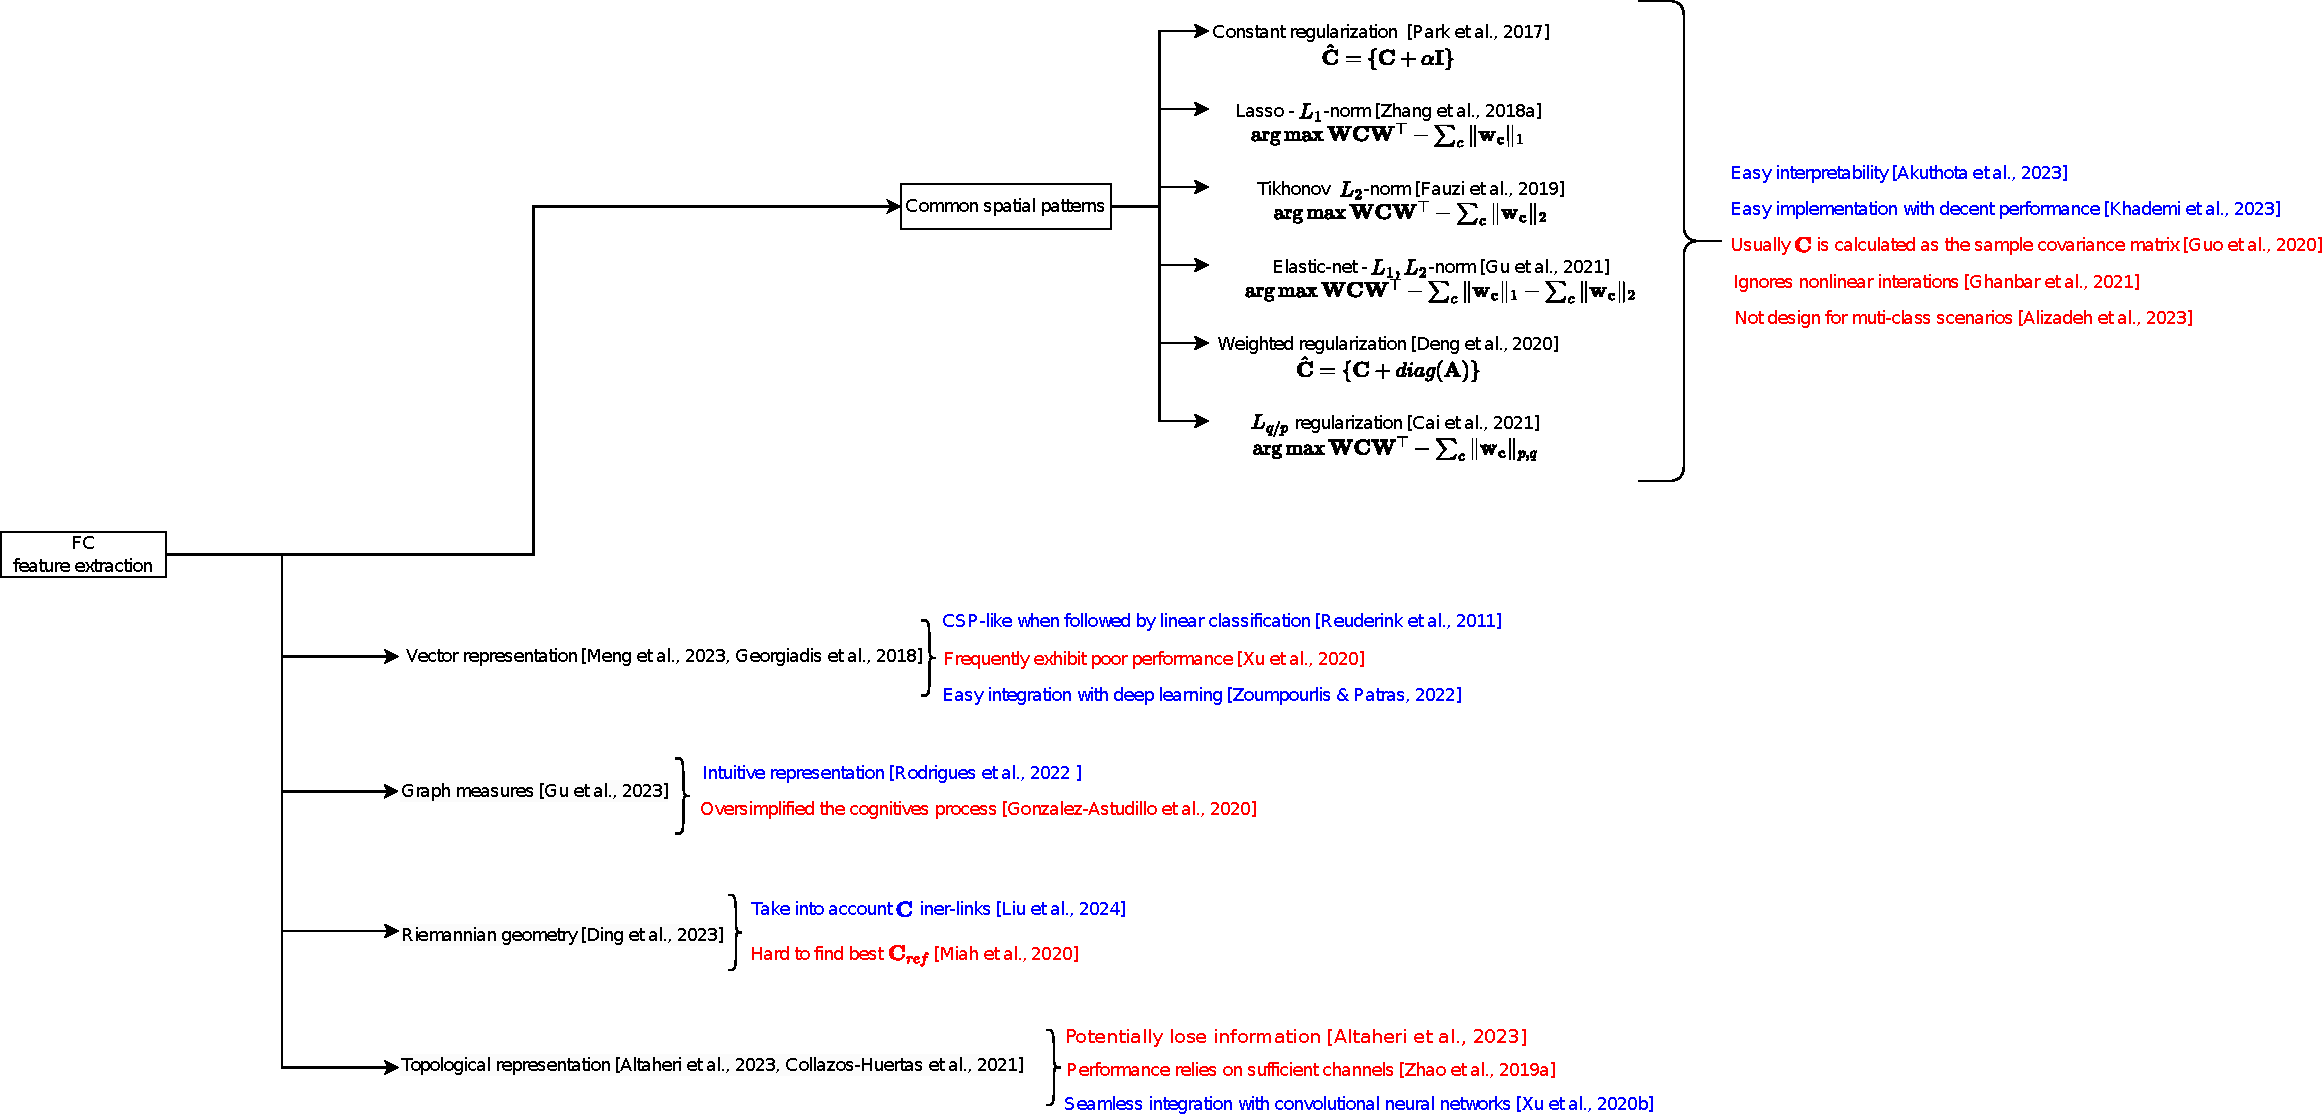
\includegraphics{Figures/state_of_art/sota1_FE}}
        \caption{Four feature extraction approaches for decoding FC in EEG-based MI-BCI: common spatial patterns, FC vectorization, topological representations, and Riemannian geometry \label{fig:sota1_FE}}

\end{figure}

Undoubtedly, CSP is the most extensive feature extraction technique that typically utilizes the simple correlation adjacency matrix to decode connectivities into distinct features, distinguishing between MI classes \cite{miljevic2022electroencephalographic, guo2020eeg}. While it allows direct interpretability using linear spatial filters, its effectiveness is limited as it relies on sample covariance \cite{akuthota2023eeg, darvish2021correlation}. CSP requires sufficient sample data and is susceptible to noise, leading to spurious connectivities and overfitting \cite{khademi2023review}. Consequently, two main approaches to regularization techniques have been explored. The first involves regularizing the covariance matrix through either constant regularization \cite{park2017filter} or weighted regularization, which impacts each channel differently \cite{deng2020local}. The second approach regularizes the projection matrix $\Vec{W}$, specifically, lasso using the $L_1$-norm \cite{zhang2018new}, Tikhonov with the $L_2$-norm \cite{fauzi2019energy}, Elastic-net combining $L_1$ and $L_2$ norms \cite{gu2021common}, and the $L_{q/p}$ regularization, which applies the $q/p$ norm \cite{cai2021single}. Despite the numerous attempts to mitigate spurious connectivities and overfitting, CSP-based techniques often overlook the nonlinearity interactions between EEG signals \cite{ghanbar2021correlation}. Furthermore, they do not offer a direct multi-class scenario \cite{alizadeh2023multi}. 

Other methodologies, such as vectorizing the adjacency matrix, leverage the symmetry of indirect FC to extract the upper triangular values, which contain insights about the mental state \cite{meng2023rhythmic, georgiadis2018exploiting}. As exhibited in \cite{reuderink2011subject}, it has been demonstrated that when vectorizing is paired with linear classification, it mimics the CSP approach. This strategy allows us to classify directly from the values of the FC matrix. Moreover, vectorizing is easily adaptable to new deep learning approaches, ensuring a seamless integration \cite{zoumpourlis2022covmix}. However, this approach is prone to overfitting and often exhibits poor performance \cite{xu2020tangent}. Since FC can be represented as graphs, various studies have employed graph measures as a feature to differentiate between MI classes \cite{gu2023decoding}. In particular, global measures, such as Characteristic path, global efficiency, and clustering coefficient, alongside node measures like local efficiency, nodal centrality, and degree centrality, have been used as features \cite{desbois2021functional, rodrigues2022can}. Nonetheless, graph measures offer oversimplified brain functioning features, often resulting in weak performance, especially in subjects with noisy EEG signals \cite{gonzalez2020network}.

So far, we have primarily discussed FC representations in Euclidean spaces, which do not account for the internal link interactions between signals in the adjacency matrix. Therefore, Riemannian geometry, which leverages the links between the coefficients of symmetric and positive definite (SPD) matrices, has been proposed \cite{freer2019adaptive}. This particular branch of differential geometry allows each matrix to be represented by a point in the manifold $\cal{M}$, where scalar products can be defined in an Euclidean tangent space \cite{mishra2018novel}. Therefore, the distance between two FC matrices can be approximately measured in this tangent space and be used as a feature to distinguish between two MI tasks \cite{ding2023study}. However, the main drawback of Riemannian geometry is the necessity for a reference matrix, typically obtained from the average of all the adjacency matrices, where minor changes can significantly affect the distance \cite{miah2020motor}.

On the other hand, imaging techniques have gained popularity due to the recent success of convolutional neural networks (CNNs) \cite{xu2020learning}. That is why some studies have used a topological representation of the FC connectivity to benefit from the easy integration with CNNs \cite{collazos2021deep}. While often achieving competitive performance, this approach heavily depends on the number of channels and suffers from potential information loss when projecting the adjacency matrix into a 2D topoplot \cite{zhao2019multi,altaheri2023deep}.

In summary, techniques such as CSP and vectorizing give different methodologies for feature extraction, each with advantages and disadvantages. CSP is a widely recognized extraction strategy that uses a correlation adjacency matrix to find linear spatial filters. However, it heavily relies on sample covariance and is susceptible to noise. Conversely, vectorizing the adjacency matrix lets us classify directly from the FC matrix values and is easily integrated with deep learning approaches. Nevertheless, both methods are susceptible to overfitting, resulting in inferior performance. Riemannian geometry provides a possible solution by allowing each matrix to represent a point on the manifold $\cal{M}$. However, it necessitates a reference matrix, making it sensitive to minor changes. The topological representation of FC connectivity integrates well with convolutional neural networks, often demonstrating competitive performance. However, it heavily relies on the number of channels and can potentially lose information when projecting the adjacency matrix into a 2D topoplot. 


\subsection{Subject-Specific EEG Representation for MI-BCI \label{sec:sota2}}

In recent years, there has been an increase in the number of methodologies introduced to handle the problem of artifacts in EEG-based MI-BCI systems \cite{kotte2020methods}. Techniques such as Canonical Correlation Analysis (CCA), Principal Component Analysis (PCA), and Independent Component Analysis (ICA) have become common tools to remove contaminated components from EEG signals \cite{stergiadis2022bss}. Notably, CCA has been identified as particularly effective in removing various artifacts \cite{rashid2020current,lahane2019review}. In addition, spatial methodologies like Common Average Reference (CAR) and Surface Laplacian (SL) have also been used to reduce noise \cite{uribe2019correntropy}. However, despite the effectiveness of these techniques, they might introduce complications by adding noise into other sensors \cite{mridha2021brain}. This problem occurs because the implemented filter removes the average electrical activity from neighboring sensors, leading to alterations in the original signal information \cite{xu2018wavelet}. \changes{On ther other hand, Deep Learning (DL) strategies have shown no significant difference in testing results between models with and without clasical artifact removing strategies. This suggest that merly using DL models may be sufficient to handle artifcat removal \cite{hassanpour2019novel,altaheri2023deep}}. Generally, DL methods can be subcategorized based on the nature of their inputs, which may be raw EEG data or handcrafted features such as statistical measures, graph measures, spectral images, and topological representations. Furthermore, the input dimension, which could be a vector, matrix, or tensor representation, also contributes to the categorization. The type of architecture employed also serves as a basis for differentiating DL, thus forming groups such as discriminative, representative, and generative models. The following section reviews the strengths and weaknesses of each model class.

\subsubsection{Input Formulation in Deep Learning}

Regarding input formulation, DL techniques can be categorized into models that depend on handcraft-based feature representation or raw EEG signals, as depicted in \cref{fig:sota2_input}. Furthermore, the input can be classified according to its dimensionality, represented as either a vector, matrix, or tensor.

The simplest handcraft method employs either graph measurements or signal statistics, with the input represented as a vector $[N_q]$, where $N_q$ denotes the total number of features \cite{gu2023decoding}. Graph measurements are metrics that capture significant properties of connectivity architectures, such as node degree and cluster coefficient. On the other hand, signal statistics represent fundamental characteristics of the signal, like mean, variance, skewness, and kurtosis. Despite the simple nature of these methods, they tend to oversimplify the complex processes within EEG signals, leading to less accurate performance \cite{gonzalez2020network}.

Spectral image approaches are another classification of techniques in which spectrograms, visual representations of the spectrum of frequencies of a signal as it varies with time, are used to portray the EEG signal as spatial-temporal-frequency images. Numerous methods can be employed to extract the spectrogram as a matrix. These techniques include Empirical Mode Decomposition (EMD), a method that decomposes a signal into intrinsic oscillatory components called intrinsic mode functions \cite{tang2020motor}; PSD, a measure of signal's power content versus frequency \cite{ma2020dwt}; Fast Fourier Transform (FFT), a mathematical technique that transforms a function of time into a function of frequency \cite{hassanpour2019novel}; Wavelet Transform (WT), a mathematical transform used to split up data, functions or signals into different frequency components \cite{ortiz2019new}; Short-Time Fourier Transform (STFT), a technique for determining the sinusoidal frequency and phase content of local sections of a signal as it changes over time \cite{tayeb2019validating}; and Continuous Wavelet Transform (CWT), a tool that allows for the analysis of non-stationary signals at many different scales or sizes \cite{lee2019application}.

Once the spectrogram is derived, several strategies can be executed for its organization, ranging from simple two-dimensional matrices to complex three-dimensional tensors. The possible permutations include but are not limited to the following formats: $[N_c \times N_f]$ \cite{ma2020dwt}, $[N_c \times N_c \times N_t]$ \cite{wang2019stable}, $[N_c \times N_c \times (N_f+N_t)]$  \cite{collazos2023posthoc}, $[N_c \times N_c]$ \cite{kwon2021visual}, $[(N_f + N_c)\times N_t]$ \cite{zhang2020motor}, $[(N_t + N_c)\times N_f]$ \cite{kant2020cwt}, $[(N_t + N_c)\times (N_f + N_c)]$ \cite{alwasiti2020motor}, and $[N_c \times N_f \times N_t]$ \cite{miao2020spatial}. $N_t$ stands for time points, $N_c$ number of channels, and $N_f$ number of filters. The selected arrangement largely depends on the specific requirements of the EEG signal analysis and the complexity of the information to be analyzed. Each organizational structure offers a unique perspective and could be more effective for different tasks or scenarios. Despite this flexibility, it's worth noting that there is a potential loss of information in each representation \cite{altaheri2023deep}

\begin{figure}[h!]
    \centering
    \resizebox{1.0\linewidth}{!}{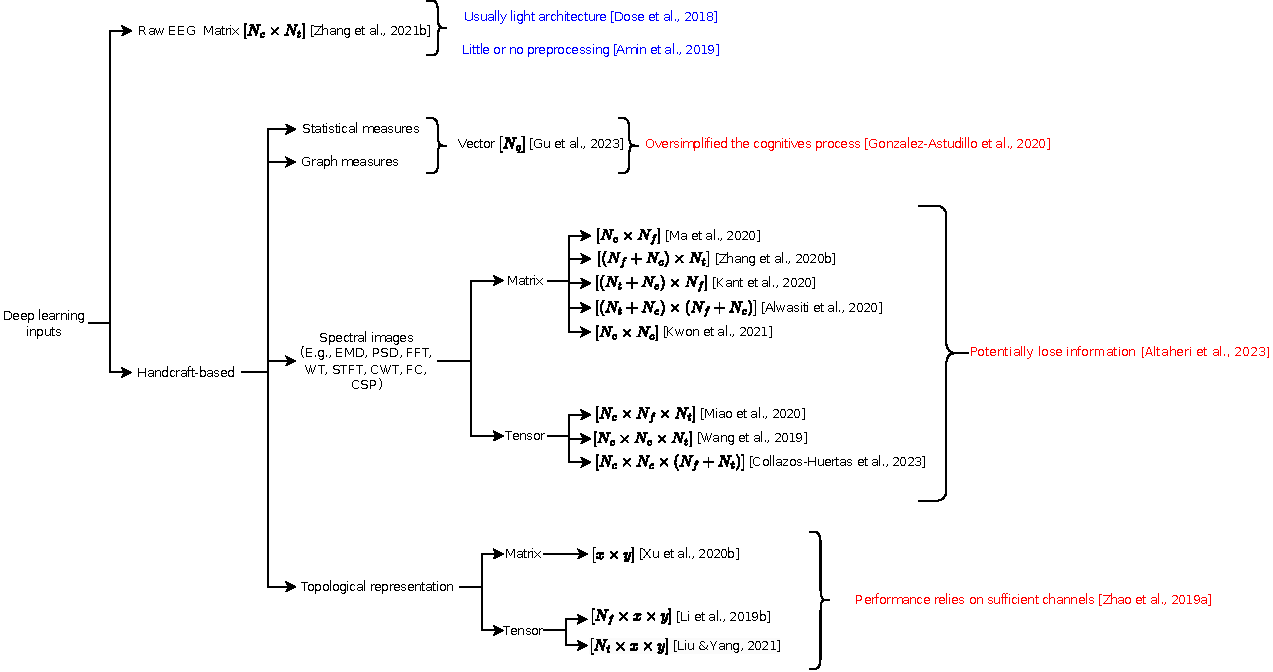
\includegraphics{Figures/state_of_art/sota2_input_v2.pdf}}
        \caption{Deep Learning techniques grouped by input formulation. Featuring handcraft-based feature representation and raw EEG signals, this categorization further divides the input according to dimensions such as vector, matrix, and tensor. The weaknesses and strengths of each form are also highlighted \label{fig:sota2_input}}
\end{figure}

The topological representation approach maps the brain's connectivity to topoplots and then processes them through deep learning architectures. These representations can range from matrix forms to more complex tensor forms. They can appear in the form of a matrix $[x \times y]$ \cite{xu2020learning}, where $x$ and $y$ represent the dimensions of the pixel array in the topoplot image. However, higher dimensional structures are favored to capture the complexities in signal variability across the frequency and time axes. For instance, tensors are often utilized to hold additional dimensions. These structures come in the forms of $[N_f \times x \times y]$ \cite{li2019novel}, and $[N_t \times x \times y]$ \cite{liu2021densely}. These formats offer a more volumetric view of the information in the EEG data. However, it is to be noted that while these approaches can maintain a greater amount of information, they also heavily rely on a sufficient number of channels being available \cite{zhao2019imaging}.

DL models that directly utilize raw EEG data as input are increasingly becoming widespread owing to their unique advantages \cite{dose2018end}. The typical input structure for these models is in the form of a matrix $[N_c \times N_t]$. This configuration allows the model to process the data directly without requiring complex transformations or feature extractions. One of the major strengths of this approach is the lightweight architecture associated with the model. As a result, raw EEG-based DL models are less computationally intensive and require little to no preprocessing \cite{amin2019deep}.

 
\subsubsection{Deep Learning Architectures}

Depending on the underlying architecture, DL models can be categorized into discriminative models, representative models, and generative models, as displayed in \cref{fig:sota2_DLA}. 

Discriminative models encompass architectures such as Multilayer Perceptron (MLP) \cite{amin2019deep}, a type of feedforward artificial neural network model that maps sets of input data onto appropriate outputs. It's worth noting, however, that MLP is relatively inefficient at extracting spatial information \cite{hossain2023status, altaheri2023deep}. Convolutional Neural Networks (CNN) \cite{zhang2021adaptive} represent another type of discriminative model. Like the connectivity pattern between neurons in the human brain, CNNs process data using a grid-like topology. This architecture is particularly apt for automatic spatial, temporal, and spectral filtering \cite{kollHod2023deep}. Furthermore, CNNs readily integrate with other architectures \cite{sharma2023recent}. Discriminative models also include Recurrent Neural Networks (RNN), which utilize previous model states in current inputs. RNNs branch into Long Short-Term Memory (LSTM) units \cite{kumar2019brain} and Gated Recurrent Units (GRU) \cite{luo2018exploring}. LSTM networks, by using gates, can selectively filter temporal information to effectively capture longer dependencies. On the other hand, GRU is a variation of LSTM with only two gates and fewer parameters. Despite these advantages, such networks can lead to inefficiencies when used independently \cite{kostiukevych2021convolutional} and can still face vanishing gradient issues \cite{gao2022parallel}. Graph Neural Networks (GNN), tailored specifically for MI-BCI \cite{ju2023graph}, have emerged recently. These networks extend the concept of Neural Networks (NNs) to graph-structured data, typically involving complex architectures \cite{kulatilleke2023towards}.

\begin{figure}[h!]
    \centering
    \resizebox{1.0\linewidth}{!}{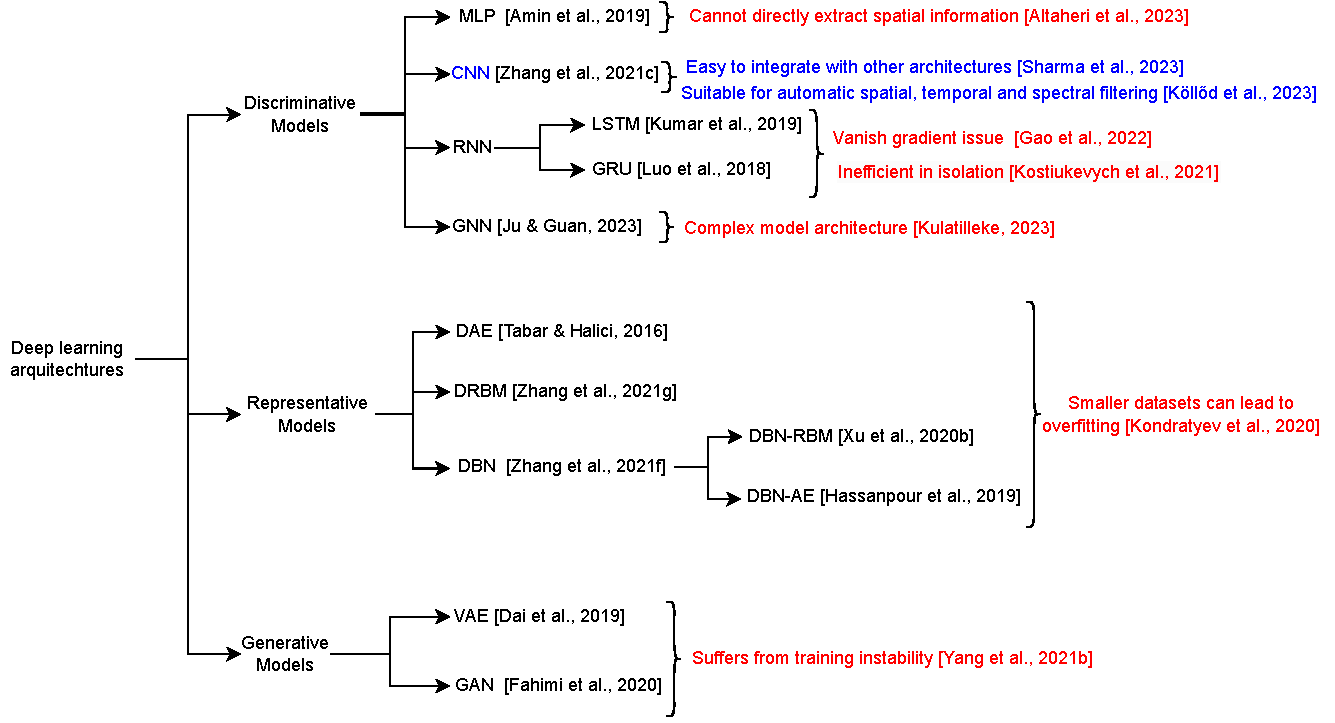
\includegraphics{Figures/state_of_art/sota2_DLAV2.pdf}}
        \caption{Deep learning model categories sorted into discriminative, representative, and generative groups, showcasing their weaknesses and strengths \label{fig:sota2_DLA}}
\end{figure}

Concerning representative models, architectures such as Deep Autoencoders (DAE) \cite{tabar2016novel}, Deep Restrictive Boltzmann Machines (DRBM) \cite{zhang2021survey}, and Deep Belief Networks (DBN) are included~\cite{zhang2021combination}. DAE is a specific variant of a Stacked autoencoder and one of the pioneering deep learning techniques. DBN is a generative probabilistic model with deep architecture that contains many layers of hidden units, and DRBN is a deep learning model capable of learning complex temporal behavior. DBN can further be integrated with autoencoders DBN-AE \cite{hassanpour2019novel} and restrictive Boltzmann machines DBN-RBM \cite{xu2020recognition}. However, These models are prone to overfitting with small datasets \cite{kondratyev2020data}.

Generative models such as Variational Autoencoders (VAE) \cite{dai2019eeg} and Generative Adversarial Networks (GAN) \cite{fahimi2020generative} are also prevalent among DL architectures. VAEs are extensions of traditional autoencoders that learn to encode input data into a set of parameters from which data can be generated, while GANs consist of two networks, a generator and a discriminator, that compete against each other to become more accurate in their predictions. However, GANS and VAE suffer from training instability \cite{yang20214}.

Finally, hybrid architectures integrated from different models have also been developed to exploit the strengths of different models and mitigate their weaknesses, In practice, hybrid methods for EEG-based MI-BCI syetms include CNN+LTSM \cite{zhang2021hybrid}, GAN + CNN \cite{zhang2020data}, LSTM+SVM \cite{kumar2021opticalb}, CNN+SVM \cite{alazrai2019deep}, GNN+CNN \cite{tang2023graph}, and DBN + CNN \cite{dai2019eeg}. to note that CNN is the most relevant architecture being used for most of the hybrid approach since they can extract relevant spatial, temporal, and spectral features.


\subsection{Interpretability Strategies in MI-BCI \label{sec:sota3}}

To enhance the interpretability of models in MI-BCI systems that handle multiple domain features, the primary goal is to unmask the complexity underlying deep learning models and leverage this knowledge to improve model predictions. As shown in \cref{fig:sota3_methods}, XAI methodologies can generally be divided into two categories: post-hoc and intrinsic. 

\begin{figure}[h!]
    \centering
    \resizebox{1.0\linewidth}{!}{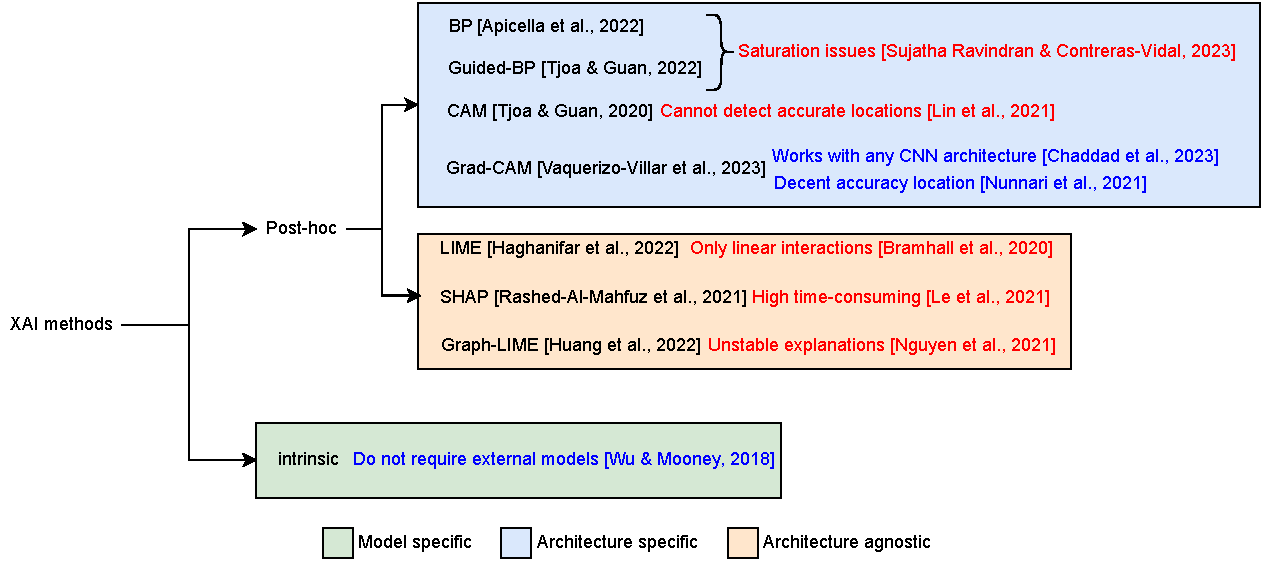
\includegraphics{Figures/state_of_art/sota3_methods.pdf}}
        \caption{Explanability strategies for machine learning and deep learning approaches\label{fig:sota3_methods}}
\end{figure}

Intrinsic models, characterized by their explicit model structures and inherent interpretability, include logistic/linear regression, Random Fourier Features (RFF), k-Nearest Neighbors (KNN), and Bayesian methods \cite{chaddad2023survey}. These techniques directly offer interpretability and do not require external models, but they are model-specific \cite{wu2018faithful}. 

In contrast, post-hoc methods aim to interpret existing models' outputs, serving as a key link between machine predictions and human comprehension \cite{speith2022review}. These methods are further subdivided into architecture-agnostic and architecture-specific approaches. 

Architecture-agnostic interpretation methods work toward creating simple, interpretable approximations of predictive models. They can be applied across many machine learning models without specific prerequisites. These methods focus on understanding a model's behavior and pinpointing the key factors that contribute to their predictions. An example is LIME \cite{haghanifar2022covid}, which offers interpretability but is limited to only linear interactions \cite{bramhall2020qlime}. Another method, SHAP \cite{rashed2021deep}, assigns each feature an importance value for a given prediction, providing a unified measure of feature importance. However, it can be computationally intensive and time-consuming \cite{le2021machine}. Lastly, Graph-LIME \cite{huang2022graphlime} provides explanations based on graph theory but may generate unstable explanations \cite{nguyen2021evaluation}.

Conversely, architecture-specific interpretation methods are custom-shaped to fit particular architectures. The latter leverages shared structural elements among a subset of models \cite{selvaraju2017grad}. For instance, Backpropagation (BP) \cite{apicella2022toward} is commonly utilized as an interpretation method, but it can succumb to saturation issues~\cite{sujatha2023empirical}. Likewise, Guided Backpropagation (Guided-BP) \cite{tjoa2022evaluating} is another architecture-specific method but shares similar challenges with BP methods.

In addition, Class Activation Mapping (CAM) \cite{tjoa2020survey} aims to emphasize influential regions within classification tasks but struggles with precise localization \cite{lin2021you}. The Gradient-weighted Class Activation Mapping (Grad-CAM) method \cite{vaquerizo2023explainable} ameliorates this issue and provides decent location accuracy \cite{chaddad2023survey, nunnari2021overlap}. However, CAM-style methods, including Grad-CAM and its variants, are traditionally limited to a network's final layers \cite{jiang2021layercam, selvaraju2017grad, chattopadhay2018grad}. Gradient-based methods like Grad-CAM often yield noisy maps, limiting interpretability \cite{omeiza2019smooth}. While perturbation-based techniques provide insights, they are computationally intensive \cite{fong2017interpretable}. CAM methods offer single-sample visual explanations but are dependent on model architecture \cite{wang2020score}. Layer CAM, an enhancement of Grad-CAM, offers better input region localization but may overlook important information from earlier layers. \cite{jiang2021layercam}

On the other hand, quantitative explanations are essential for evaluating the performance of XAI models and comparing them numerically \cite{hassija2023interpreting}. Metrics such as Average drop $\%$, increase confidence $\%$, and win $\%$ can be used to measure the quality of explanations and identify the strengths and weaknesses of different XAI methods \cite{naidu2020cam}. This allows researchers to develop more accurate and interpretable XAI models that can be used to solve a wider range of problems.

In conclusion, each interpretability method has its strengths and limitations and provides unique insights into the inner workings of machine learning models \cite{rahate2022multimodal}. Therefore, the choice of an interpretability method should mirror each application's specific requirements and constraints.

\subsection{Summary}

In general, nonlinear methods for extracting indirect functional connectivity data from trial-based EEG signals achieve acceptable accuracy. However, their complexity makes them susceptible to noise, resulting in spurious connectivity. Meanwhile, DL methods capably handle artifacts and EEG representations, necessitating minimal preprocessing. Specifically, models based on CNNs are well-suited for automatic spatial, temporal, and spectral filtering. Furthermore, incorporating intrinsic and post-hoc interpretability strategies into these models could enhance their transparency and interpretability.
\chapter{Aims}

The analysis above leads us to the following general and specific objectives:

\section{General Objective}

To develop a single-trial indirect functional connectivity framework, accompanied by regularized deep learning approaches, to extract pertinent subject-specific non-linear spatio-temporal-frequency patterns from non-stationary EEG data, improving the MI-BCI system's accuracy and interpretability.

\section{Specific Objectives}

\begin{itemize}
	\item[1] To develop a single-trial indirect FC for enhanced nonlinear feature extraction, preserving the spatio-temporal-frequency interpretability while favoring the classification performance in MI-BCI and avoiding spurious connectivities.
 
	\item[2] To extend the proposed single-trial FC within a deep learning scheme that handles artifacts and EEG representations, necessitating minimal preprocessing efforts from raw signals.
 
	\item[3] To develop a transparency and interpretability strategy dedicated to MI-BCI classification that emphasizes spatial-temporal-spectral pattern domains, incorporating a qualitative and quantitative relevance analysis assessment.
\end{itemize}

\chapter{Outline and Contributions}

\begin{figure}[h!]
    \centering
    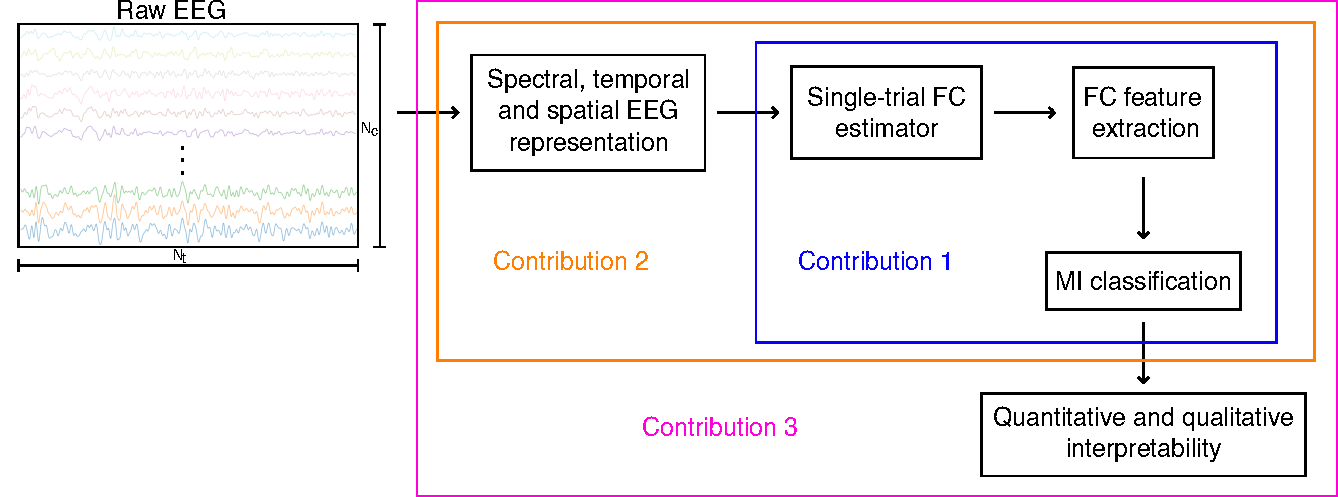
\includegraphics[scale=0.6]{Figures/outline_and_contributions/general_contributions.pdf}
    \caption{Schematic display of the main thesis contributions, including the single-trial FC estimator and feature extraction, an end-to-end approach from EEG representations to MI classification, and quantitative and qualitative strategies for model interpretation\label{fig:img_gen_outline}}
\end{figure}

This chapter offers a clear introduction to the main contributions of this thesis, as illustrated in \cref{fig:img_gen_outline}. Firstly, it presents a novel single-trial FC estimator designed to improve MI classification tasks by addressing nonlinearities, intersubject variability, and spurious connections. Secondly, it introduces a comprehensive end-to-end approach aimed at extracting subject-specific spectral, temporal, and spatial EEG representations, which can aid in reducing the incidence of artifacts and establishing more relevant connections. Lastly, the chapter suggests qualitative and quantitative interpretability strategies for comparing DL EEG-based MI-BCI models, alongside a regularization approach to further mitigate spurious connections.


\section{Single-Trial FC for Enhancing MI-BCI Classification \label{sec:contribution1}}

As referenced in \cref{sec:singlefc}, implementing robust single-trial FC estimators and streamlined feature extraction methodologies is paramount to improving the MI-BCI model's accuracy without affecting its interpretability. More specifically, successful strategies must be devised to confront the complex issues related to spurious connectivities, non-linearity, non-stationarity, and inter-subject variability. Upon a comprehensive examination of the state-of-the-art in \cref{sec:sota1}, our proposal addresses non-stationarity by implementing short sliding windows, which are presumed weakly stationary, at varying widths \cite{gaur2021sliding}. The problem of non-linearity integrating a Gaussian kernel that has proven effective against non-linear situations \cite{gunawardena2023kernel}. Specifically, we propose an extension of Bochner's theorem \cite{bochner2020harmonic}, named the Kernel-based Cross-Spectral FC (KCS-FC),  to approximate the cross-spectral distribution of a stationary kernel function by using a weighted sum of Gaussian-based pairwise relationships within different sub-band filters and time windows. The challenge of inter-subject variability using a sub-band filtering technique \cite{mammone2023autoencoder}. Moreover, a vectorization representation is proposed for FC feature extraction, mainly because of its seamless integration with end-to-end models and its responses, which are closely similar to those in CSP under linear classifier scenarios \cite{meng2023rhythmic, zoumpourlis2022covmix}. To restrict spurious connectivities, we propose introducing an elastic-net regularization mechanism \cite{tay2023elastic}. \cref{fig:contribution1} shows a graphical depiction of this proposition.  


\section{Automatic Subject-Specific EEG Representation for MI-BCI}

As referenced in \cref{sec:problem2}, it is crucial to implement models that do not strongly rely on handcrafted subject-specific EEG representations. These kinds of models can help get rid of artifacts and reduce false connections, which will make MI-BCI more accurate, especially for people who do not do well with their BCI (BCI inefficiency) \cite{park2023improving}. The following method is proposed based on the state-of-the-art exploration in \cref{sec:sota2}. First, DL strategies are proposed due to their significant efficacy in dealing with artifact removal, further mitigating the problem of spurious connectivities\cite{altaheri2023deep, huang2023discrepancy, hassanpour2019novel}. Specifically, end-to-end DL models using raw EEG as inputs are preferred as they require little or no preprocessing and allow for light architectures \cite{dose2018end, amin2019deep}. Secondly, we propose using a CNN layer to automatically extract temporal and spectral features \cite{altaheri2023deep, craik2019deep, musallam2021electroencephalography, lawhern2018eegnet}. Additionally, spatial extraction is performed by creating a custom layer incorporating the KCS-FC function from our contribution in \cref{sec:contribution1}. This contribution is illustrated in \cref{fig:contribution2}.


\section{Qualitative and Quantitative Post-Hoc and Intrinsic Explainability}

As referenced in \cref{sec:problem3}, transparency and interpretability strategies in MI-BCI models are critical in healthcare and medical decision-making scenarios \cite{miotto2018deep, xiao2018opportunities}. Additionally, measuring the effectiveness of new MI-BCI models with qualitative and quantitative explainability from multiple domains is not easy. The following explainable AI strategy is proposed based on the state-of-the-art exploration in \cref{sec:sota3}. Firstly, we propose qualitative interpretability using Layer-CAM post-hoc interpretability, which is based on the Grad-CAM method and can work with any CNN architecture \cite{chaddad2023survey}. It presents a decent accuracy location \cite{nunnari2021overlap} and highlights spatiotemporal triggers in the raw EEG. Intrinsic interpretability is achieved by checking the last layer weights, resulting in channel importance that is represented as a topoplot. Secondly, for quantitative interpretation, we borrow the concept of average drop \cite{naidu2020cam} from image processing to compare different MI-BCI models. \changes{To compare results we include a regularization technique based on Renyi's entropy to analyze how interpretability is affected when the cross-information potential of the internal FC of the KCS-FCnet is maximized}. This leads to the proposed Interpretable Regularized Kernel Cross-Spectral Functional Connectivity Network (IRKCS-FCnet) depicted in \cref{fig:contribution3}.


\chapter{Materials and Methods}


\section{EEG-based Motor Imagery Datasets}\label{sec:dataset}

We employed three motor-related public databases to appraise the performance of the proposed single-trial KCS-FC, automatic subject-specific EEG representations KCS-FCnet, and the qualitative and quantitative explainability IRKCS-FCnet. These databases are described in detail below.

\subsection{BCI Competition IV Dataset IIa - DBI MI}

\subsubsection{Protocol Design}

BCI Competition IV dataset IIa (DBI MI) is a public dataset \footnote{\url{www.bbci.de/competition/iv}} created by researchers in \cite{brunner2008bci} that contains EEG recordings from nine subjects ($M=9$) who were instructed to perform four MI tasks ($N_y=4$) (left hand, right hand, feet, and tongue). Data were gathered in two days within six runs, yielding three runs per day. One run contains $12$ trials per task, which were recorded by $C=22$ channels, for a total of $R=144$ trials of each label per subject, where each channel was sampled at \changes{$250 Hz$}. To estimate Electro-oculography (EOG) influence, EEG recording with opened, closed, and in-movement eyes lasting five minutes at the beginning of each session as illustrated in \cref{fig:bci2a_schema}.

\begin{figure}[!h]
  \centering
  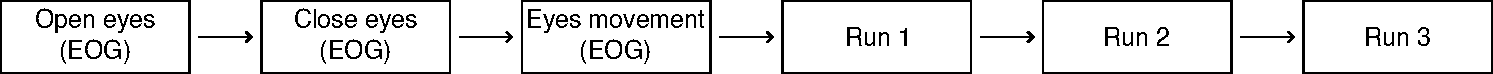
\includegraphics[width=\linewidth]{Figures/preliminaries/BCI2a_schema.pdf}
  \caption{Schema representing a one-day session of EEG data collection for the DBI MI \label{fig:bci2a_schema}}
\end{figure}

Subjects were instructed to sit on a comfortable armchair in front of a computer screen. \cref{fig:BCI2aprotocol} shows the seven-second MI protocol. The start was indicated by a short acoustic warning and a cross on a black screen for two seconds, then an arrow pointing left, right, down, or up indicated to the subjects to perform the desired MI task. Furthermore, the subjects were asked to continue the MI task until the cross disappeared \changes{three} seconds later. Afterward, a black screen indicated a short break until the beep and the cross reappeared, and a new trial started.

\begin{figure}[h!]
\centering
    \resizebox{0.5\linewidth}{!}{
\begin{tikzpicture}
\draw[draw=black] (0,0) rectangle ++(2,2) node[pos=.5] {Black screen};
\draw[draw=black] (2,0) rectangle ++(3,3) node[pos=.5] {Motor Imagery};
\draw[draw=black] (5,0) rectangle ++(2,2) node[pos=.5] {Black screen};
\draw[dashed,draw=black] (7,0) rectangle ++(1,2) node[pos=.5] {Break};

% \draw[draw=red] (2.5,-0.2) rectangle ++(2,1) node[pos=.5] {\textcolor{red}{\small{Analysis span}}};
% \draw[dashed,draw=red] (2.5,0) -- (2.5,-1) node[pos=1.5] {\textcolor{red}{$2.5$}};
% \draw[dashed,draw=red] (4.5,0) -- (4.5,-1) node[pos=1.5] {\textcolor{red}{$4.5$}};

\draw [-stealth](0,0) -- (9,0) node[below,pos=1.05] {$s$};

\draw[dashed,draw=black] (0,0) -- (0,-0.5) node[pos=1.5] {$0$};
\draw[dashed,draw=black] (1,0) -- (1,-0.5) node[pos=1.5] {$1$};
\draw[dashed,draw=black] (2,0) -- (2,-0.5) node[pos=1.5] {$2$};

\draw[-stealth,dashed,draw=red] (2,0) -- (2,3.5) node[pos=1.1] {\textcolor{red}{Cue}};

\draw[-stealth,dashed,draw=red] (0,0) -- (0,2.5) node[pos=1.1] {\textcolor{red}{Beep}};

\draw[dashed,draw=black] (3,0) -- (3,-0.5) node[pos=1.5] {$3$};
\draw[dashed,draw=black] (4,0) -- (4,-0.5) node[pos=1.5] {$4$};
\draw[dashed,draw=black] (5,0) -- (5,-0.5) node[pos=1.5] {$5$};
\draw[dashed,draw=black] (6,0) -- (6,-0.5) node[pos=1.5] {$6$};
\draw[dashed,draw=black] (7,0) -- (7,-0.5) node[pos=1.5] {$7$};
\draw[dashed,draw=black] (8,0) -- (8,-0.5) node[pos=1.5] {$8$};
\end{tikzpicture}}
    \caption{Illustration of the seven-second DBI MI protocol used in the study. The protocol commences with a short acoustic warning and a cross shown on a screen for two seconds, followed by an arrow indicating the type of MI task to be performed. The black screen marks a brief break interval between tasks.
    \label{fig:BCI2aprotocol}}
\end{figure}

\subsubsection{Data Recording}

Twenty-two Ag/AgCI electrodes with an inter-electrode distance of 3.5cm and an international $10-20$ montage were used to acquire brain activity as shown in \cref{fig:montagebci2a}. All signals were monopolar recorded with the left mastoid electrode serving as a reference and the right one as ground. Activity was sampled at \changes{$250 s$} and bandpass filtered between \changes{$0.5 Hz$} and \changes{$100 Hz$}. The amplifier sensitivity was set to $100 \mu V$. Additionally, a notch filter centered at \changes{$50 Hz$} was applied to diminish electrical line noise. Moreover, three monopolar EOG channels were also included with the same specifications but with amplifier sensitivity set to $1mV$. This was done with the intention of subsequent artifact removal strategies. An expert visually inspected all EEG recordings to mark trials with high noise artifacts.

\begin{figure}[h!]
\centering
    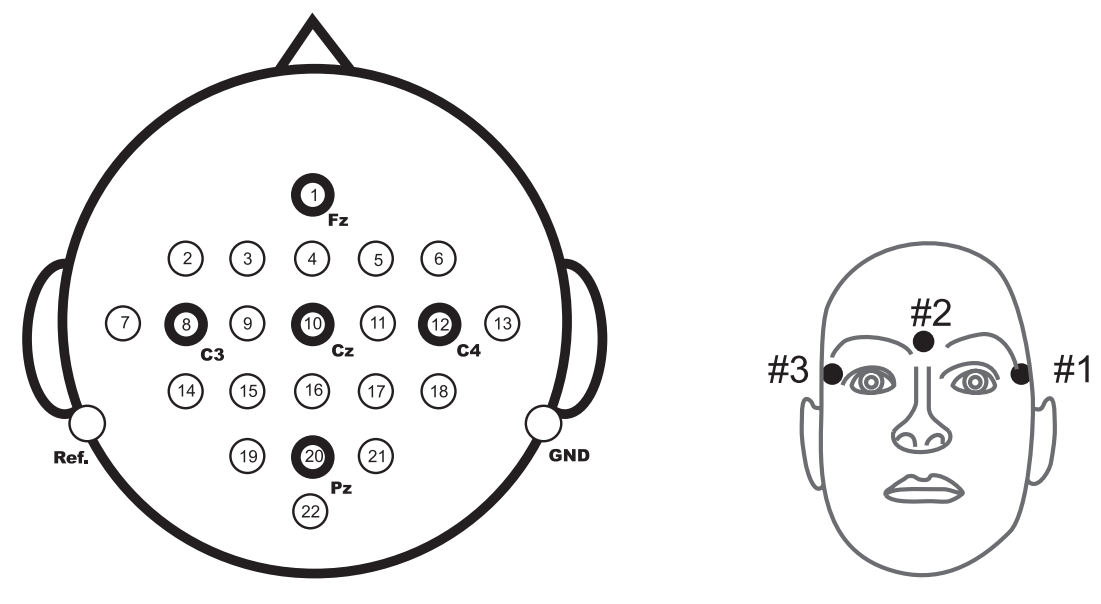
\includegraphics[width=0.6\linewidth]{Figures/preliminaries/bcielectrodes.PNG}
    \caption{Illustration of the electrode montage including the left image adhering to the international 10-20 system used for acquiring brain activity and the right image showing the montage of the three monopolar EOG channels employed for subsequent artifact removal. \textbf{Source:} \cite{brunner2008bci}. \label{fig:montagebci2a}}
\end{figure}

\subsection{Gamma Motor Execution Database---DBII ME}

\subsubsection{Protocol Design}

We explore the data that are publicly available at (\url{https://gin.g-node.org/robintibor/high-gamma-dataset}); this collection is a dataset collected by authors in \cite{schirrmeister2017deep}, obtained from $14$ healthy subjects ($6$ female, $2$ left-handed, age $27.2\pm 3.6$) with four-second trials of executed movements divided into $13$ runs per subject and ($R = 260$) trials were performed to collect each movement and rest. The four classes were movements of either the left hand, the right hand, both feet, and rest (no movement, but the same type of visual cue as the other classes). Visual cues were presented while using a monitor outside the cabin, which was visible through the shielded window. A fixation point was attached at the center of the screen. The subjects were instructed to relax, fixate on the mark, and keep as still as possible during the motor execution task. The tasks were as follows: Depending on the direction of a gray arrow that was shown on the black background. The subjects had to clench their toes (downward arrow), repetitively, perform sequential finger-tapping of their left (leftward arrow) or right (rightward arrow) hand, or relax (upward arrow). The movements were selected to require little proximal muscular activity while still being complex enough to keep subjects involved. Within the \changes{$4 s$} trials, the subjects performed the repetitive movements at their own pace, which had to be maintained as long as the arrow was showing. Per run, $80$ arrows were displayed for \changes{$4 s$} each, with $3$ to \changes{$4 Hz$} of continuous random inter-trial interval as shown in \cref{fig:gamma_time}

\begin{figure}[h!]
\centering
    \resizebox{1.0\linewidth}{!}{
\begin{tikzpicture}
\draw[draw=black] (0,0) rectangle ++(4,2) node[pos=.5] {Motor Execution $\#1$};
\draw[dashed,draw=black] (4,0) rectangle ++(4,2) node[pos=.5] {Random Break};
\draw[dashed,draw=black] (7,0) -- (7,2) node[pos=1.5] {};


% \draw[draw=red] (2.5,-0.2) rectangle ++(2,1) node[pos=.5] {\textcolor{red}{\small{Analysis span}}};
% \draw[dashed,draw=red] (2.5,0) -- (2.5,-1) node[pos=1.5] {\textcolor{red}{$2.5$}};
% \draw[dashed,draw=red] (4.5,0) -- (4.5,-1) node[pos=1.5] {\textcolor{red}{$4.5$}};

\draw [-stealth](0,0) -- (9,0) node[below,pos=1.05] {$s$};

\draw[dashed,draw=black] (0,0) -- (0,-0.5) node[pos=1.5] {$0$};

\draw[-stealth,dashed,draw=red] (0,0) -- (0,2.5) node[pos=1.1] {\textcolor{red}{Cue}};


\draw[dashed,draw=black] (4,0) -- (4,-0.5) node[pos=1.5] {$4$};

\draw[dashed,draw=black] (7,0) -- (7,-0.5) node[pos=1.5] {$7$};
\draw[dashed,draw=black] (8,0) -- (8,-0.5) node[pos=1.5] {$8$};


\end{tikzpicture}}
    \caption{Schema representing a one-run session of EEG data collection for the DBII ME
    \label{fig:gamma_time}}
\end{figure}

\subsubsection{Data Recording}

The EEG setup for the experiment comprised active electromagnetic shielding, high-resolution low-noise amplifiers, an actively shielded $128$-channel EEG cap, and full optical decoupling. All devices were battery-powered and communicated via optical fibers. Data were collected from $44$ sensors covering the motor cortex as shown in \cref{fig:eeg_gamma}, and were sampled at a rate of \changes{$500 Hz$}. Subjects were accommodated comfortably in a dimly lit Faraday cabin where they received visual cues on a monitor approximately $1$ meter away. A fixation point served as the focal point during the motor execution exercises. Subjects were instructed to stay still, relax, and limit body movements like blinking and swallowing to inter-trial intervals to ensure optimal data collection. The combined effect of the electromagnetic shielding and the comfortable, dimly lit environment helped maintain data coherence.

\begin{figure}[h!]
\centering
    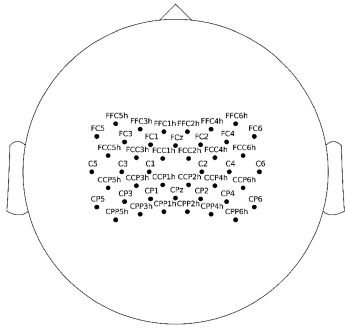
\includegraphics[width=0.4\linewidth]{Figures/preliminaries/gammaelectrodes.PNG}
    \caption{Positioning of the 44 sensors on the EEG cap, covering the motor cortex used for data collection in the motor execution experiment. Source: \cite{borra2019eeg} \label{fig:eeg_gamma}}
\end{figure}

\subsection{MI BCI EEG Giga Science Database - DBIII MI}

MI BCI EEG Giga Science database (DBIII MI) is an ideal choice for our validation as it has been widely used in the field of MI classification and has been shown to provide a robust benchmark for evaluating the performance of different models \cite{cho2017eeg}.
However, for the purpose of our study, we will only consider 50 subjects who met the minimum requirement of having at least 100 EEG trials recorded.

\subsubsection{Protocol Design}

This collection, publicly available at \footnote{\url{http://gigadb.org/dataset/100295}} and produced by researchers in \cite{cho2017eeg} holds EEG recordings obtained from 52 subjects ($M=52$), holding 19 females, performing two MI tasks ($N_y=2$) (left and right hand). $50$ were right-handed and $2$ left-handed. Data were gathered in a laboratory with a noise level between $37$ and $39$ decibels during one of the next time slots, T1 (9:30–12:00), T2 (12:30–15:00), T3 (15:30–18:00), or T4 (19:00–21:30).  $R=100$ trials of each label per subject were recorded by $C=64$ channels, where each channel was sampled at \changes{$512 Hz$}. Furthermore, EMG and EEG were recorded simultaneously with the same system and sampling rate to check actual hand movements.

\begin{figure}[h!]
\centering
    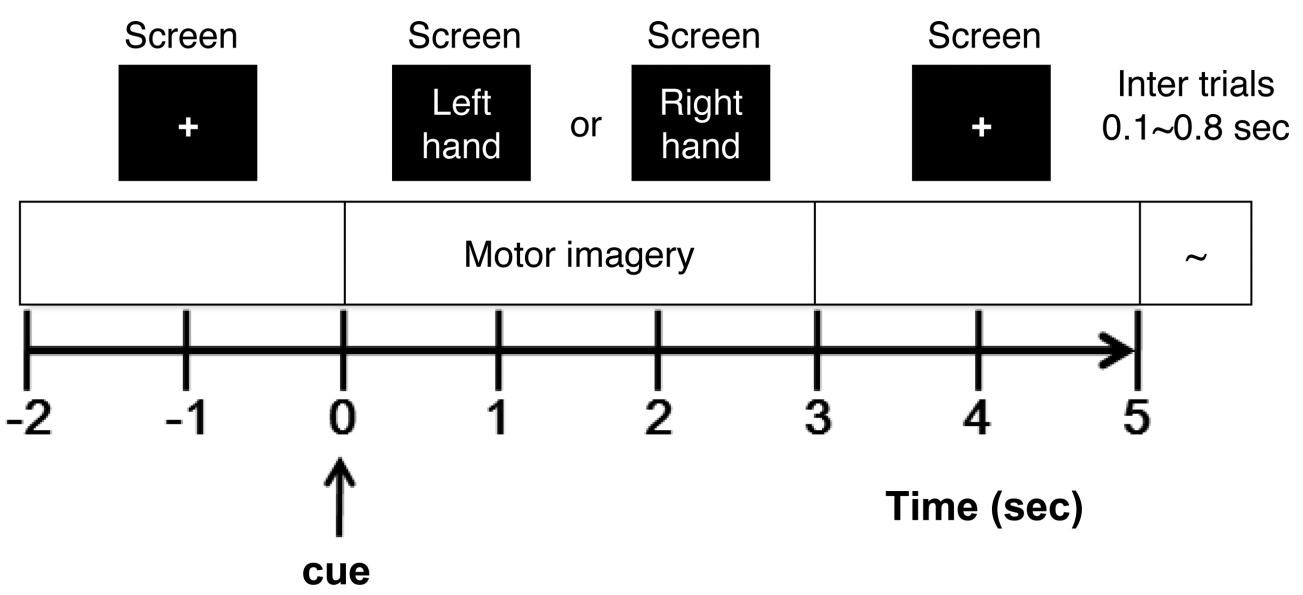
\includegraphics[width=0.7\linewidth]{Figures/preliminaries/protocol_giga.PNG}
    \caption{Diagram illustrating the experiment protocol involving motor imagery tasks. The figure shows the sequence of prompting, performing, and break periods in a single run. Source: \cite{cho2017eeg} \label{fig:protocol_giga}}
\end{figure}

The experiment involved non-motor related and motor imagery tasks, starting with data collected under six different types of noise conditions: eye blinking, eye movements, head movement, chewing, and resting state. Each noise type was recorded twice for five seconds, except for the resting state condition, which was recorded for 60 seconds. Following the noise data collection, subjects performed MI tasks, which were prompted via a monitor and conducted as per a protocol explained in \cref{fig:protocol_giga}. Each trial in this experiment stage started with a 2-second fixation on a cross displayed on a black screen. This was followed by a cue indicating a right or left-hand MI task. During the MI task, subjects were instructed to imagine the sensation of touching each finger of the designated hand with the thumb, beginning from the index finger and proceeding sequentially to the little finger. This emphasis on the kinesthetic rather than the visual aspect ensured that the subjects were indeed imagining the motor task. The MI task continued for 3 seconds, after which a blank screen signaled a rest period. This recovery interval lasted randomly between 2.1 and 2.8 seconds.

This task, break, and recovery cycle was repeated 20 times to form a complete run. Each subject performed between five and six such runs. After each run, a cognitive questionnaire was given to the subjects as an additional data collection point. Data quality was ensured by labeling and excluding trials with high voltage magnitude, classified as "bad trials", from the final analysis. Lastly, to maintain the engagement and motivation of the subjects, they were provided with feedback on the accuracy of their task performance after each run.



\subsubsection{Data Recording}

For this experiment, EEG data were collected using 64 active Ag/AgCl electrodes, according to a 64-channel montage based on the international 10-10 system and recorded at a sampling rate of \changes{$512 Hz$} as illustrated in Figure \ref{fig:dataset_sensors}. The Biosemi ActiveTwo system was employed for EEG collection, with instructions for left or right-hand motor imagery being presented through the BCI2000 system 3.0.2. EMG was recorded concurrently with EEG to verify actual hand movements, with two electrodes attached to the flexor digitorum profundus and extensor digitorum on each arm. For every participant, the EEG channel locations were recorded with a 3D coordinate digitizer; positions were averaged from three measurements to accommodate for possible hand tremors.

\begin{figure}[h!]
\centering
        \resizebox{0.4\linewidth}{!}{%% Creator: Inkscape 1.2.2 (b0a8486541, 2022-12-01), www.inkscape.org
%% PDF/EPS/PS + LaTeX output extension by Johan Engelen, 2010
%% Accompanies image file 'reference_plot_2.pdf' (pdf, eps, ps)
%%
%% To include the image in your LaTeX document, write
%%   \input{<filename>.pdf_tex}
%%  instead of
%%   \includegraphics{<filename>.pdf}
%% To scale the image, write
%%   \def\svgwidth{<desired width>}
%%   \input{<filename>.pdf_tex}
%%  instead of
%%   \includegraphics[width=<desired width>]{<filename>.pdf}
%%
%% Images with a different path to the parent latex file can
%% be accessed with the `import' package (which may need to be
%% installed) using
%%   \usepackage{import}
%% in the preamble, and then including the image with
%%   \import{<path to file>}{<filename>.pdf_tex}
%% Alternatively, one can specify
%%   \graphicspath{{<path to file>/}}
%% 
%% For more information, please see info/svg-inkscape on CTAN:
%%   http://tug.ctan.org/tex-archive/info/svg-inkscape
%%
\begingroup%
  \makeatletter%
  \providecommand\color[2][]{%
    \errmessage{(Inkscape) Color is used for the text in Inkscape, but the package 'color.sty' is not loaded}%
    \renewcommand\color[2][]{}%
  }%
  \providecommand\transparent[1]{%
    \errmessage{(Inkscape) Transparency is used (non-zero) for the text in Inkscape, but the package 'transparent.sty' is not loaded}%
    \renewcommand\transparent[1]{}%
  }%
  \providecommand\rotatebox[2]{#2}%
  \newcommand*\fsize{\dimexpr\f@size pt\relax}%
  \newcommand*\lineheight[1]{\fontsize{\fsize}{#1\fsize}\selectfont}%
  \ifx\svgwidth\undefined%
    \setlength{\unitlength}{558.00027682bp}%
    \ifx\svgscale\undefined%
      \relax%
    \else%
      \setlength{\unitlength}{\unitlength * \real{\svgscale}}%
    \fi%
  \else%
    \setlength{\unitlength}{\svgwidth}%
  \fi%
  \global\let\svgwidth\undefined%
  \global\let\svgscale\undefined%
  \makeatother%
  \begin{picture}(1,0.99999946)%
    \lineheight{1}%
    \setlength\tabcolsep{0pt}%
    \put(0,0){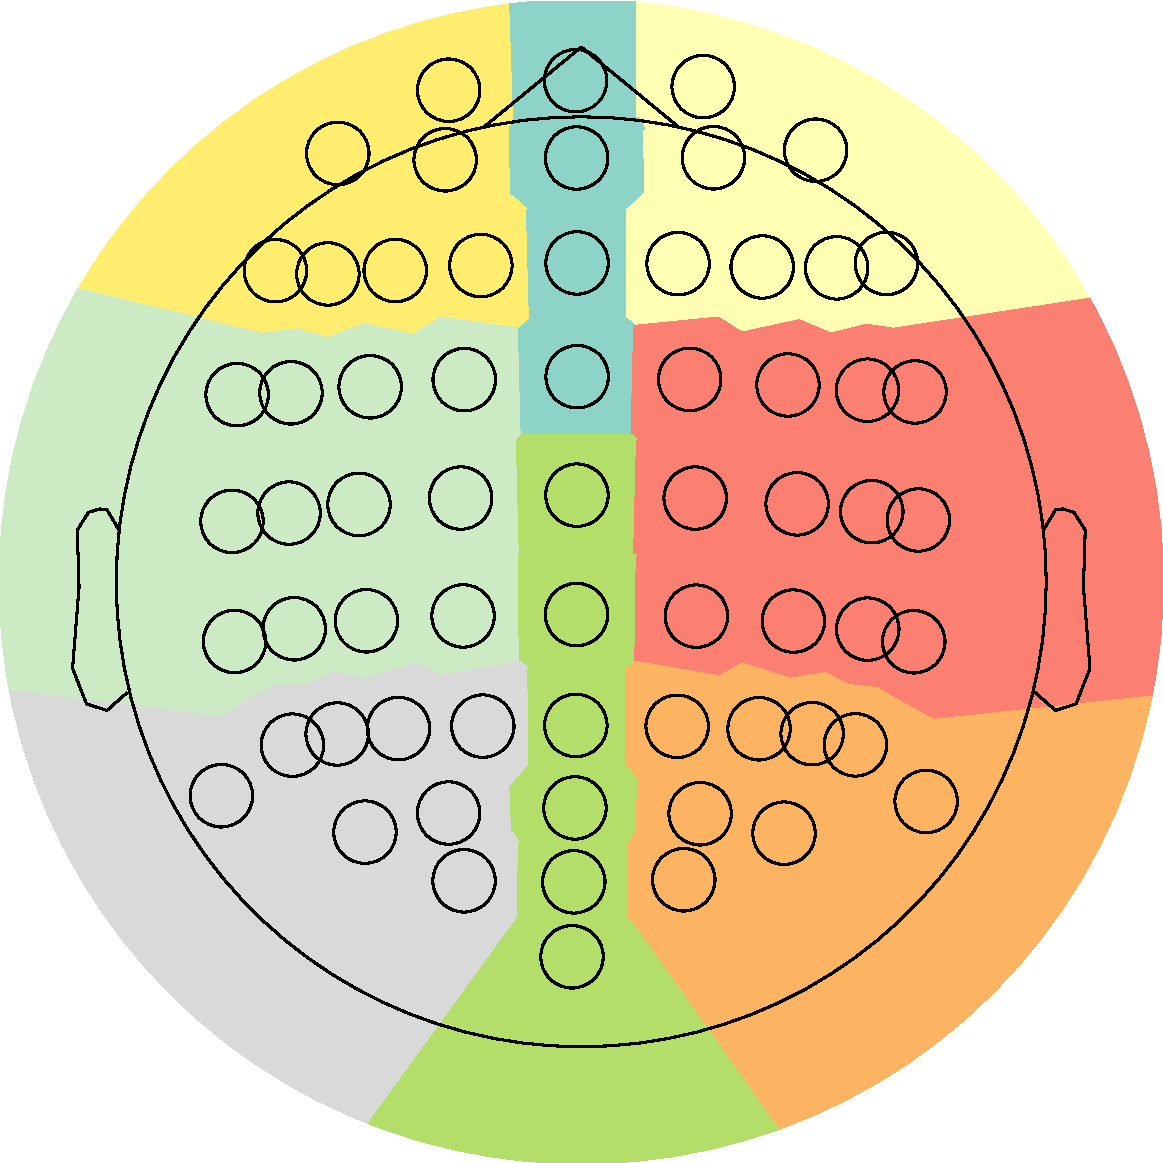
\includegraphics[width=\unitlength,page=1]{Figures/Objective_2/reference_plot_2.pdf}}%
    \put(0.36652085,0.91688558){\color[rgb]{0,0,0}\makebox(0,0)[lt]{\lineheight{1.25}\smash{\begin{tabular}[t]{l} \Large Fp1\end{tabular}}}}%
    \put(0.4768886,0.92508034){\color[rgb]{0,0,0}\makebox(0,0)[lt]{\lineheight{1.25}\smash{\begin{tabular}[t]{l} \Large Fpz\end{tabular}}}}%
    \put(0.58545766,0.9199935){\color[rgb]{0,0,0}\makebox(0,0)[lt]{\lineheight{1.25}\smash{\begin{tabular}[t]{l} \Large Fp2\end{tabular}}}}%
    \put(0.27059445,0.86251654){\color[rgb]{0,0,0}\makebox(0,0)[lt]{\lineheight{1.25}\smash{\begin{tabular}[t]{l} \Large AF7\end{tabular}}}}%
    \put(0.3629916,0.85707131){\color[rgb]{0,0,0}\makebox(0,0)[lt]{\lineheight{1.25}\smash{\begin{tabular}[t]{l} \Large AF3\end{tabular}}}}%
    \put(0.47724471,0.85857267){\color[rgb]{0,0,0}\makebox(0,0)[lt]{\lineheight{1.25}\smash{\begin{tabular}[t]{l} \Large AFz\end{tabular}}}}%
    \put(0.59373517,0.85882249){\color[rgb]{0,0,0}\makebox(0,0)[lt]{\lineheight{1.25}\smash{\begin{tabular}[t]{l} \Large AF4\end{tabular}}}}%
    \put(0.68165218,0.86525161){\color[rgb]{0,0,0}\makebox(0,0)[lt]{\lineheight{1.25}\smash{\begin{tabular}[t]{l} \Large AF8\end{tabular}}}}%
    \put(0.22412503,0.76166001){\color[rgb]{0,0,0}\makebox(0,0)[lt]{\lineheight{1.25}\smash{\begin{tabular}[t]{l} \Large F7\end{tabular}}}}%
    \put(0.26927017,0.7588327){\color[rgb]{0,0,0}\makebox(0,0)[lt]{\lineheight{1.25}\smash{\begin{tabular}[t]{l} \Large F5\end{tabular}}}}%
    \put(0.32722637,0.76178557){\color[rgb]{0,0,0}\makebox(0,0)[lt]{\lineheight{1.25}\smash{\begin{tabular}[t]{l} \Large F3\end{tabular}}}}%
    \put(0.40084017,0.76607436){\color[rgb]{0,0,0}\makebox(0,0)[lt]{\lineheight{1.25}\smash{\begin{tabular}[t]{l} \Large F1\end{tabular}}}}%
    \put(0.48479265,0.76828852){\color[rgb]{0,0,0}\makebox(0,0)[lt]{\lineheight{1.25}\smash{\begin{tabular}[t]{l} \Large Fz\end{tabular}}}}%
    \put(0.57052921,0.76768551){\color[rgb]{0,0,0}\makebox(0,0)[lt]{\lineheight{1.25}\smash{\begin{tabular}[t]{l} \Large F2\end{tabular}}}}%
    \put(0.64291322,0.76483078){\color[rgb]{0,0,0}\makebox(0,0)[lt]{\lineheight{1.25}\smash{\begin{tabular}[t]{l} \Large F4\end{tabular}}}}%
    \put(0.70693925,0.76411092){\color[rgb]{0,0,0}\makebox(0,0)[lt]{\lineheight{1.25}\smash{\begin{tabular}[t]{l} \Large F6\end{tabular}}}}%
    \put(0.74976654,0.7678815){\color[rgb]{0,0,0}\makebox(0,0)[lt]{\lineheight{1.25}\smash{\begin{tabular}[t]{l} \Large F8\end{tabular}}}}%
    \put(0.18501382,0.65500385){\color[rgb]{0,0,0}\makebox(0,0)[lt]{\lineheight{1.25}\smash{\begin{tabular}[t]{l} \Large FT7\end{tabular}}}}%
    \put(0.230178,0.65661815){\color[rgb]{0,0,0}\makebox(0,0)[lt]{\lineheight{1.25}\smash{\begin{tabular}[t]{l} \Large FC5\end{tabular}}}}%
    \put(0.29831107,0.66177952){\color[rgb]{0,0,0}\makebox(0,0)[lt]{\lineheight{1.25}\smash{\begin{tabular}[t]{l} \Large FC3\end{tabular}}}}%
    \put(0.37926054,0.6679257){\color[rgb]{0,0,0}\makebox(0,0)[lt]{\lineheight{1.25}\smash{\begin{tabular}[t]{l} \Large FC1\end{tabular}}}}%
    \put(0.47752226,0.67045104){\color[rgb]{0,0,0}\makebox(0,0)[lt]{\lineheight{1.25}\smash{\begin{tabular}[t]{l} \Large FCz\end{tabular}}}}%
    \put(0.57317084,0.66816088){\color[rgb]{0,0,0}\makebox(0,0)[lt]{\lineheight{1.25}\smash{\begin{tabular}[t]{l} \Large FC2\end{tabular}}}}%
    \put(0.65770736,0.66333128){\color[rgb]{0,0,0}\makebox(0,0)[lt]{\lineheight{1.25}\smash{\begin{tabular}[t]{l} \Large FC4\end{tabular}}}}%
    \put(0.72608603,0.65883651){\color[rgb]{0,0,0}\makebox(0,0)[lt]{\lineheight{1.25}\smash{\begin{tabular}[t]{l} \Large FC6\end{tabular}}}}%
    \put(0.76814418,0.65733992){\color[rgb]{0,0,0}\makebox(0,0)[lt]{\lineheight{1.25}\smash{\begin{tabular}[t]{l} \Large FT8\end{tabular}}}}%
    \put(0.18640365,0.54603203){\color[rgb]{0,0,0}\makebox(0,0)[lt]{\lineheight{1.25}\smash{\begin{tabular}[t]{l} \Large T7\end{tabular}}}}%
    \put(0.23460137,0.55313947){\color[rgb]{0,0,0}\makebox(0,0)[lt]{\lineheight{1.25}\smash{\begin{tabular}[t]{l} \Large C5\end{tabular}}}}%
    \put(0.29478238,0.56055995){\color[rgb]{0,0,0}\makebox(0,0)[lt]{\lineheight{1.25}\smash{\begin{tabular}[t]{l} \Large C3\end{tabular}}}}%
    \put(0.38224136,0.56605545){\color[rgb]{0,0,0}\makebox(0,0)[lt]{\lineheight{1.25}\smash{\begin{tabular}[t]{l} \Large C1\end{tabular}}}}%
    \put(0.48341184,0.56856097){\color[rgb]{0,0,0}\makebox(0,0)[lt]{\lineheight{1.25}\smash{\begin{tabular}[t]{l} \Large Cz\end{tabular}}}}%
    \put(0.58396329,0.56604577){\color[rgb]{0,0,0}\makebox(0,0)[lt]{\lineheight{1.25}\smash{\begin{tabular}[t]{l} \Large C2\end{tabular}}}}%
    \put(0.67165057,0.56107375){\color[rgb]{0,0,0}\makebox(0,0)[lt]{\lineheight{1.25}\smash{\begin{tabular}[t]{l} \Large C4\end{tabular}}}}%
    \put(0.73581692,0.55433585){\color[rgb]{0,0,0}\makebox(0,0)[lt]{\lineheight{1.25}\smash{\begin{tabular}[t]{l} \Large C6\end{tabular}}}}%
    \put(0.77680978,0.54719732){\color[rgb]{0,0,0}\makebox(0,0)[lt]{\lineheight{1.25}\smash{\begin{tabular}[t]{l} \Large T8\end{tabular}}}}%
    \put(0.18230964,0.44267411){\color[rgb]{0,0,0}\makebox(0,0)[lt]{\lineheight{1.25}\smash{\begin{tabular}[t]{l} \Large TP7\end{tabular}}}}%
    \put(0.23266377,0.45363629){\color[rgb]{0,0,0}\makebox(0,0)[lt]{\lineheight{1.25}\smash{\begin{tabular}[t]{l} \Large CP5\end{tabular}}}}%
    \put(0.29480849,0.46048839){\color[rgb]{0,0,0}\makebox(0,0)[lt]{\lineheight{1.25}\smash{\begin{tabular}[t]{l} \Large CP3\end{tabular}}}}%
    \put(0.37790608,0.46465505){\color[rgb]{0,0,0}\makebox(0,0)[lt]{\lineheight{1.25}\smash{\begin{tabular}[t]{l} \Large CP1\end{tabular}}}}%
    \put(0.47667086,0.46584238){\color[rgb]{0,0,0}\makebox(0,0)[lt]{\lineheight{1.25}\smash{\begin{tabular}[t]{l} \Large CPz\end{tabular}}}}%
    \put(0.57863054,0.46445265){\color[rgb]{0,0,0}\makebox(0,0)[lt]{\lineheight{1.25}\smash{\begin{tabular}[t]{l} \Large CP2\end{tabular}}}}%
    \put(0.66201097,0.46025166){\color[rgb]{0,0,0}\makebox(0,0)[lt]{\lineheight{1.25}\smash{\begin{tabular}[t]{l} \Large CP4\end{tabular}}}}%
    \put(0.7260133,0.45330943){\color[rgb]{0,0,0}\makebox(0,0)[lt]{\lineheight{1.25}\smash{\begin{tabular}[t]{l} \Large CP6\end{tabular}}}}%
    \put(0.76651151,0.442468){\color[rgb]{0,0,0}\makebox(0,0)[lt]{\lineheight{1.25}\smash{\begin{tabular}[t]{l} \Large TP8\end{tabular}}}}%
    \put(0.1773533,0.31000801){\color[rgb]{0,0,0}\makebox(0,0)[lt]{\lineheight{1.25}\smash{\begin{tabular}[t]{l} \Large P9\end{tabular}}}}%
    \put(0.23846259,0.35349394){\color[rgb]{0,0,0}\makebox(0,0)[lt]{\lineheight{1.25}\smash{\begin{tabular}[t]{l} \Large P7\end{tabular}}}}%
    \put(0.27698556,0.36310273){\color[rgb]{0,0,0}\makebox(0,0)[lt]{\lineheight{1.25}\smash{\begin{tabular}[t]{l} \Large P5\end{tabular}}}}%
    \put(0.32967442,0.36774008){\color[rgb]{0,0,0}\makebox(0,0)[lt]{\lineheight{1.25}\smash{\begin{tabular}[t]{l} \Large P3\end{tabular}}}}%
    \put(0.40221594,0.36989273){\color[rgb]{0,0,0}\makebox(0,0)[lt]{\lineheight{1.25}\smash{\begin{tabular}[t]{l} \Large P1\end{tabular}}}}%
    \put(0.48343935,0.37045952){\color[rgb]{0,0,0}\makebox(0,0)[lt]{\lineheight{1.25}\smash{\begin{tabular}[t]{l} \Large Pz\end{tabular}}}}%
    \put(0.56946187,0.36971499){\color[rgb]{0,0,0}\makebox(0,0)[lt]{\lineheight{1.25}\smash{\begin{tabular}[t]{l} \Large P2\end{tabular}}}}%
    \put(0.63988534,0.36763877){\color[rgb]{0,0,0}\makebox(0,0)[lt]{\lineheight{1.25}\smash{\begin{tabular}[t]{l} \Large P4\end{tabular}}}}%
    \put(0.68556707,0.36335775){\color[rgb]{0,0,0}\makebox(0,0)[lt]{\lineheight{1.25}\smash{\begin{tabular}[t]{l} \Large P6\end{tabular}}}}%
    \put(0.72274037,0.35377449){\color[rgb]{0,0,0}\makebox(0,0)[lt]{\lineheight{1.25}\smash{\begin{tabular}[t]{l} \Large P8\end{tabular}}}}%
    \put(0.7769358,0.3050661){\color[rgb]{0,0,0}\makebox(0,0)[lt]{\lineheight{1.25}\smash{\begin{tabular}[t]{l} \Large P10\end{tabular}}}}%
    \put(0.29258972,0.27868376){\color[rgb]{0,0,0}\makebox(0,0)[lt]{\lineheight{1.25}\smash{\begin{tabular}[t]{l} \Large PO7\end{tabular}}}}%
    \put(0.36456386,0.29509967){\color[rgb]{0,0,0}\makebox(0,0)[lt]{\lineheight{1.25}\smash{\begin{tabular}[t]{l} \Large PO3\end{tabular}}}}%
    \put(0.47439325,0.29952217){\color[rgb]{0,0,0}\makebox(0,0)[lt]{\lineheight{1.25}\smash{\begin{tabular}[t]{l} \Large POz\end{tabular}}}}%
    \put(0.58088867,0.29451737){\color[rgb]{0,0,0}\makebox(0,0)[lt]{\lineheight{1.25}\smash{\begin{tabular}[t]{l} \Large PO4\end{tabular}}}}%
    \put(0.65306662,0.27776523){\color[rgb]{0,0,0}\makebox(0,0)[lt]{\lineheight{1.25}\smash{\begin{tabular}[t]{l} \Large PO8\end{tabular}}}}%
    \put(0.38419722,0.23682676){\color[rgb]{0,0,0}\makebox(0,0)[lt]{\lineheight{1.25}\smash{\begin{tabular}[t]{l} \Large O1\end{tabular}}}}%
    \put(0.47975668,0.2359459){\color[rgb]{0,0,0}\makebox(0,0)[lt]{\lineheight{1.25}\smash{\begin{tabular}[t]{l} \Large Oz\end{tabular}}}}%
    \put(0.57316751,0.23772853){\color[rgb]{0,0,0}\makebox(0,0)[lt]{\lineheight{1.25}\smash{\begin{tabular}[t]{l} \Large O2\end{tabular}}}}%
    \put(0.48340759,0.17146872){\color[rgb]{0,0,0}\makebox(0,0)[lt]{\lineheight{1.25}\smash{\begin{tabular}[t]{l} \Large Iz\end{tabular}}}}%
  \end{picture}%
\endgroup%
}
    \caption{Sensor positions in a $10${--}$10$ placement electrode system, containing 64 channels. Besides, it highlights in color the main parts of the brain ( \legend{frontal_left} Frontal left, \legend{frontal} Frontal, \legend{frontal_right} Frontal right, \legend{central_right} Central right, \legend{posterior_right} Posterior right, \legend{posterior} Posterior, \legend{posterior_left} Posterior left, \legend{central_left} Central left)}
    \label{fig:dataset_sensors}
\end{figure}


\section{Theoretical Background}

In this section, we introduce the mathematical formulation of relevant related concepts used throughout this study.


\subsection{Motor Imagery Classification from EEG Signals}

\changes{MI involves the neural simulation of a movement that, although not physically executed, activates the same areas of the brain as actual movements. EEGs capture these activations, and machine learning models can be built to interpret these signals, allowing the prediction of human actions purely from the EEGs.}

\changes{From the mathematical perspective, let $\{\mat{X}_r\}_{r=1}^{R}$ be a multi-channel EEG observation from trial $r$, where each element $\mat{X}_r = \{\ve{x}_r^c  \in \Real^{N_t}\}_{c=1}^{N_c} $ contains $N_t \in \Natural$ time instants and $N_c \in \Natural$ number of channels. Moreover, there exists a function $\func{F}$ \eqref{eq:model} that exactly maps each trial $\mat{X}_r$ into the label space $y_r \in \{0, 1, \cdots, N_y\}$ representing the type of motor imagery with $N_y \in \Natural$ denoting the number of classes. The goal of EEG-MI classification is to find the best possible estimation function $\hat{\func{F}}(\cdot; \ve{w})$ that approximates the true function $\func{F}$ in \eqref{eq:model}, depending on a set of trainable parameters denoted as $\ve{w}$}

\begin{equation}\label{eq:model}
\func{F}: \mat{X}_r \mapsto y_r \quad \forall r \in \{1, \ldots, R\}    
\end{equation}



\subsubsection{Performance Measurement}

Performance measurement is necessary to evaluate the effectiveness of an EEG signal MI classification model. There are several commonly used metrics to measure the performance of such models, including Accuracy, Kappa coefficient, and the Area Under the Receiver Operating Characteristic Curve (AUC-ROC).

\textbf{Accuracy}: is the proportion of trials where a model correctly predicts the class label, represented as:

\begin{equation}
Acc = \frac{1}{R} \sum_{r=1}^{R} \Kronecker{\hat{y}_r}{y_r}
\end{equation}


where $\hat{y}_r$ and $y_r$ are the predicted and actual class labels, respectively, for the $r$-th trial, and $\Kronecker{\cdot}{\cdot}$ is the Kronecker delta function.

\textbf{Kappa Coefficient}: or Cohen’s kappa, measures inter-rater agreement. It considers the agreement occurring by chance, hence, providing a more robust metric than simple accuracy. Given a confusion matrix, the kappa coefficient can be calculated as:

\begin{equation}
\kappa = \frac{p_o - p_e}{1 - p_e}    
\end{equation}

where $p_o$ is the relative observed agreement, and $p_e$ is the hypothetical probability of random chance agreement.

\textbf{AUC-ROC curve}: AUC represents the probability that a classifier will rank a randomly chosen positive instance higher than a randomly chosen negative instance. The ROC curve is created by plotting the true positive rate (TPR) against the false positive rate (FPR) at various threshold settings.

For instance, let $\hat{p}_r$ be the predicted probability of the $r$-th trial belonging to the positive class. Then $\hat{p}_r = \sigma(\hat{\func{F}}(\mat{X}_r); \ve{w})$, where $\sigma(x) = 1/(1 + \exp(-x))$ is the logistic function that transforms the model output into a probability. Therefore, The TPR (or sensitivity) and FPR (or 1-specificity) can be defined as follows:

\begin{equation}
    TPR = \frac{\text{TP}}{\text{P}} = \frac{\sum_{r=1}^{R} \Kronecker{\hat{y}r}{ y_r}\Kronecker{y_r}{1}}{\sum{r=1}^{R} \Kronecker{y_r}{1}}    
\end{equation}

\begin{equation}
    FPR = \frac{\text{FP}}{\text{N}} = \frac{\sum_{r=1}^{R} \Kronecker{\hat{y}_r}{ 1}\Kronecker{y_r}{0}}{\sum{r=1}^{R} \Kronecker{y_r}{0}}
\end{equation}

where TP is the number of true positives, FP is the number of false positives, P is the number of positive instances, and N is the total number of negative ones. Thus, the AUC can be computed by integrating the curve over the interval $[0,1]$. In practice, the integral is estimated by the trapezoidal rule since we only have a finite number of instances from which to construct the ROC curve. In essence, the AUC-ROC measures the model's ability to discriminate positive from negative cases.

\subsection{Stochastic Processes}

A stochastic process, in the context of MI-BCI systems, serves as a robust mathematical construct for characterizing the progression of underlying random systems over distinct periods of time. More specifically, $\ve{\chi}$ outlines the behavior of each signal. 

This process characteristically encompasses a diverse array of random variables specifically designed to mimic the dynamism inherent within these random systems. Each variable in this set is denoted as $X^c_r(t)$, and for simplicity in mathematical representation, it is rewritten as $X^c(t)$. These variables constitute drawn samples corresponding to distinct time instances $t$. Hence, with the entire set identified as $\{{x}^{c}_{t} \in \Real\}_{t=0}^{N_t}$, these sampled variables effectively encapsulate the progression of the stochastic process, from $t=0$ to $t=N_t$.

\subsubsection{Random Process Moments}
 
In the study of random processes, 'moments' are vital quantitative measures that describe data set features, including mean, variance, skewness, and kurtosis. In this context, the focus is on the first and second moments. The first moment relates to the mean, providing a central data point while the second moment relates to the variance and correlation, indicating data dispersion and the relationship between variables, respectively. These moments give a comprehensive view of the dataset's structure and dynamics.

\subsubsection{First Moment}

The first moment, also known as the expectation, of a random variable $\ve{x}^c(t)$, represents the expected value or mean of the variable. It serves as a measure of the center of the data distribution. The expectation can be mathematically defined as follows.

\begin{equation}
    \mathbb{E}\{X^{c}\} = \mu_{x^{c}} = \int_{-\infty}^{+\infty} x P_d(x^{c}) dx^{c}
\end{equation}

where $P_d(x^{c})$ is the probability density function.

\subsubsection{Second Moment}

The second moment of a random variable, often referred to as the variance, denoted as $\mathcal{R}_{X^c}$, serves as the measure of how much the potential outcomes of the variable deviate from its mean value. This quantifies the spread or dispersion of the data. The formulation for variance can be computed as follows.

\begin{equation}
  \begin{split}
    \mathcal{R}_{X^c} = \mathbb{E}\{(X^{c} - \mu_{x^{c}})^2\} &= \int_{-\infty}^{+\infty} \left( x^{c}-\mu_{x^{c}} \right) ^2 P_d(x^{c}) dx^{c} \\
    &= \mathbb{E}\{(X^{c})^2\} - (\mathbb{E}\{X^{c}\})^2
  \end{split}
\end{equation}

In the context of EEG-based MI-BCI systems, there is a common practice of centering each channel by eliminating the mean value. Consequently, when $\mu_x^{c}=0$, the variance equation can be reformulated as:

\begin{equation}
  \begin{split}
    \mathcal{R}_{X^c} = \mathbb{E}\{(X^{c})^2\} &= \int_{-\infty}^{+\infty}  (x^{c})^2 P_d(x^{c}) dx^{c} \\
    &= \mathbb{E}\{(X^{c})^2\}
  \end{split}
\end{equation}

The Covariance, another important concept intertwined with variance, measures the joint variability or spread of two random variables. It determines how much the variables change together and quantifies their dependency. If two signals $X^c$ and $X^{c'}$ are centered, $\mu_X^{c}=0$ and $\mu_X^{c'}=0$, the covariance $Cov(X^{c},^{c'})$ can be computed as follows.

\begin{equation}
  \begin{split}
    \mathcal{R}_{X^{c},X^{c'}} = \mathbb{E} \left[ X^{c} X^{c'}  \right] = \mathbb{E} \left[ X^{c} X^{c'} \right]
  \end{split}
\end{equation}

Covariance matrices are essential in many strategies used for MI-BCI, as they capture the relationships between different EEG channels $\ve{x}^c$. These relationships, found in the structure of the covariance matrix, contain relevant information regarding neuronal oscillations and synchronization, both of which are crucial aspects of MI tasks. Using covariance matrices is significant in techniques such as Common Spatial Patterns.

\subsubsection{Wide/Weak-Sense Stationarity Stochastic Processes}

A stochastic process is deemed wide-sense stationary (WSS) or weak-sense stationary if it satisfies the following two conditions.

\begin{enumerate}
    \item The mean function or the first moment of the process is constant. This implies that the expected value or the average value of the process should be constant over time and not rely on the underlying time. Mathematically, it is represented by the equation:

    \begin{equation}
        \mathbb{E}\{X^{c}(t)\} = \mu_{x^{c}} = \text{constant, for all } t
    \end{equation}

    where $\mathbb{E}\{X^{c}(t)\}$ denotes the expected value of the random process at any time instance $t$ and $\mu_{x^{c}}$ is the constant mean value.

    \item The autocorrelation function or the second moment of the process depends only on the difference in time and not the actual time. This suggests that the correlation between two variables taken at different periods should only depend on the difference between those periods. It can be mathematically expressed as follows.

    \begin{equation}
        \mathbb{E}\{(X^{c}(t_1)-\mu_{x^{c}})(X^{c}(t_2)-\mu_{x^{c}})\} = R_{X^{c}}(t_1,t_2) = R_{X^{c}}(t_2-t_1) = R_{X^{c}}(\tau)
    \end{equation}
    
    Where the autocorrelation function $R_{X^{c}}(t_1,t_2) = R_{X^{c}}(\tau)$ between two points at time instances $t_1$ and $t_2$ is only a function of their difference $\tau=(t_2 - t_1)$. 
\end{enumerate}

\subsubsection{Wiener Khinchin Theorem}

According to the Wiener Khinchin theorem, the autocorrelation function $\mathcal{R}_{X^c}(\tau)$ of a WSS random process is a Fourier transform pair with its power spectral density $P_{X^c}(f)$. This means that the autocorrelation function in the time domain corresponds to the power spectral density in the frequency domain and vice versa. This can be mathematically represented as follows.
\begin{equation}
    \mathcal{R}_{X^c}(\tau) = \int_{\Real} P_{X^c}(f) e^{j 2\pi f \tau} df
\end{equation}

Likewise, the power spectral density is given by the Fourier transform of the autocorrelation function.

\begin{equation}
    P_{X^c}(f) = \int_{\mathbb{f}} \mathcal{R}_{X^c}(\tau) e^{-j 2\pi f \tau} d\tau
\end{equation}

In the context of EEG-based MI-BCI systems, the Wiener-Khinchin theorem provides a useful tool for analyzing EEG signals. By transforming from the time domain to the frequency domain and vice versa, we gain insights into the spectral and temporal properties of the underlying stochastic processes, enabling efficient feature extraction and system identification.


\subsection{EEG Classical Feature Extraction Techniques}

The extraction of features from EEG signals is a crucial step towards decoding the information hidden within them. This step involves transforming the raw EEG data into a suitable set of features to represent the inherent properties that are key to differentiating different motor imagery classes. Let $\func{G}$ be a feature extraction function that transforms our raw EEG data into feature vectors as follows:
\begin{equation}
\ve{z}_r = \func{G}(\mat{X}_r)    
\end{equation}

where $\ve{z}_r \in \Real^{N_p}$ represents the feature vector for trial $r$ with $N_p \in \Natural$ denoting the feature size. The feature extraction function $\func{G}$ can be defined in various ways based on different feature extraction methods. The objective here is to find an optimal feature extraction function $\func{G}$ such that the features $\mat{Z}_r = \func{G}(\mat{X}_r)$ are discriminative enough for the classification of motor imagery EEG signals. After feature extraction step, the problem essentially becomes a feature-based classification problem, where we want to find a function $\hat{\func{F}}(\cdot,\ve{w})$ such that the estimated class label $\hat{y}_r = \hat{\func{F}}(\hat{\mat{z}}_r; \ve{w})$ matches the true label $y_r$ as accurately as possible.

\subsubsection{Common Spatial Patterns}

Common Spatial Pattern (CSP) is a widely used technique for extracting features from EEG signals, especially for Motor Imagery tasks. CSP helps in identifying spatial filters that maximize the difference of variance between classes, thereby being a powerful tool for classification problems. the core concept of CSP is the simultaneous diagonalization of two covariance matrices. 

For instance, provide an EEG dataset with two class sets, $X^{c}$ and $X^{c'}$, where for each class, the average covariance matrices $\Sigma_{C1}$ and $\Sigma_{C2}$ are calculated as follows. First, take the sum of the covariance matrices of each trial for the class and divide by the total number of trials in that class. If we have a total of $R_{C1}$ trials in the set $C1$, the covariance matrix for trial $r \in C1$, denoted as $\mat{\Sigma}_{r} \in \Real^{N_c \x N_c}$, can be calculated as:

\begin{equation}
\mat{\Sigma}_{r} = \frac{1}{N_{t}} \mat{X}_r \mat{X}_{r}^T;\quad \forall r \in C1
\end{equation}

where $N_{t}$ is the number of time instances and $\mat{X}_{r}^{T}$ is the transpose of the EEG data matrix for trial $r$. Thus, the average covariance matrix for class $C1$, denoted as $\mat{\Sigma}_{C1}$, is then calculated as follows:

\begin{equation}
\mat{\Sigma}_{C1} = \frac{1}{R_{C1}} \sum_{{r}=1}^{R_{C1}} \mat{\Sigma}_{r};\quad \forall r \in C1     
\end{equation}

A similar process can be followed to obtain the average covariance matrix for class $C2$.

The goal of CSP is to find a set of projection vectors (spatial filters) that could maximize the variance for one class while minimizing it for the other class as defined in \eqref{eq:CSP}.

\begin{equation}\label{eq:CSP}
\ve{w}^* = \max_{\ve{w}} \frac{\ve{w}^T \mat{\Sigma}_{C1} \ve{w}}{\ve{w}^T \mat{\Sigma}_{C2} \ve{w}}     
\end{equation}

The solution to this problem is given by the joint eigenvectors of $\mat{\Sigma}_{C1}$ and $\mat{\Sigma}_{C2}$ corresponding to the maximum and minimum eigenvalues. The transformed EEG is not directly used in classification models. Instead, a common approach is to use the log variance of the transformed signals and often take from the top and bottom few filters. First, compute the transformed signal as:

\begin{equation}
\mat{S}_r = \ve{w}^* \mat{X}_r     
\end{equation}

To calculate the final features for the CSP method, we compute the log variance of these transformed signals as follows:

\begin{equation}\label{eq:CSPfeats}
\ve{z}_r = log \left( \frac{\diag{var({\mat{S}}_{r})}}{\Tr{\diag{var(\mat{S}_{r})}}}  \right)  
\end{equation}

Where $\Tr{\cdot}$ stands for the trace operator and $\diag{\cdot}$ is the diagonal operator that extracts the elements in the principal diagonal. For instance, if we're using CSP as our feature extraction method, $\func{G}_{CSP}$ will constitute the operations involved in \eqref{eq:CSPfeats}, where the filters corresponding to the highest and lowest eigenvalues are selected, such as the from $\ve{z}_r$ we take the first $N_p/2$ and last $N_p/2$ elements, where $N_p$ is the final desired number of features. Finally, these features $\ve{z}_r$ extracted by applying the CSP technique can now be fed to the classifier for further processing.

Sure, the requested sub-subsection would be as follows:

\subsubsection{Variations of Common Spatial Patterns}

Over time, various adaptations of the CSP method have been developed to address specific issues or improve performance. These include:

\paragraph{Constant regularization:} Where a constant term is added to the sample variance for diminishing the risk of overfitting \cite{park2017filter}.

\begin{equation}
    \hat{\mathbf{C}}=\{\mathbf{C}+\alpha \mathbf{I}\}
\end{equation}

\paragraph{Lasso regularization:} This method employs a penalty equal to the absolute value of the magnitude of the coefficients. It aims to simplify the used model by forcing some coefficients to zero in the spatial linear filters \cite{zhang2018new}.

\begin{equation}
    \arg \max \mathbf{W} \mathbf{C} \mathbf{W}^{\top}-\sum_c\left\|\mathbf{w}_{{c}}\right\|_1
\end{equation}

\paragraph{Tikhonov regularization:} A squared magnitude of the spatial filter coefficients is employed as a penalty term, preventing coefficients from reaching very high values that could lead to overfitting \cite{fauzi2019energy}

\begin{equation}
    \arg \max \mathbf{W}\mathbf{C} \mathbf{W}^{\top}-\sum_c\left\|\mathbf{w}_{{c}}\right\|_2
\end{equation}

\paragraph{Elastic-net regularization:} This technique is a mix of the Lasso and Tikhonov regularizations, using both absolute and squared magnitudes, thus encompassing their benefits \cite{gu2021eeg}.

\begin{equation}
    \arg \max \mathbf{W}\mathbf{C} \mathbf{W}^{\top}-\sum_c\left\|\mathbf{w}_{{c}}\right\|_1-\sum_c\left\|\mathbf{w}_{{c}}\right\|_2
\end{equation}

\paragraph{Weighted regularization:} The diagonal of the sample covariance matrix is penalized with distinct weights to differentially shrink their effect on the spatial filters.\cite{deng2020local}

\begin{equation}
    \hat{\mathbf{C}}=\{\mathbf{C}+\operatorname{diag}(\mathbf{A})\}
\end{equation}

\paragraph{Lq/p regularization:} A generalization of Lasso and Tikhonov regularizations. It is flexible with $q$ and $p$, which can be any non-negative real numbers, providing more control over the model complexity \cite{cai2021single}.

\begin{equation}
    \arg \max \mathbf{W}\mathbf{C} \mathbf{W}^{\top}-\sum_c\left\|\mathbf{w}_{\mathbf{c}}\right\|_{p, q}
\end{equation}



Each of these versions of CSP can be selected and implemented according to the specific demands and objectives of the dataset and problem at hand.

\subsubsection{Sub-band CSP}

In practice, EEG signals not only differ in spatial patterns but also in frequency bands. Sub-band Common Spatial Pattern (SBCSP) is an extension that considers the frequency components of the EEG signals. First, it decomposes the original EEG signals into various frequency bands before applying the CSP method to each band individually. The generated sub-band CSP features are then concatenated to create a more robust feature vector that includes both spatial and spectral information, resulting in improved performance in classifying motor imagery tasks.

Suppose we define a band-pass filter $\func{H}_f$ that decomposes an EEG signal into the frequency band $f \in \Omega$, where $\Omega$ is a set of filters. Thus, the filter operation can be represented as:

\begin{equation}
\tilde{\mat{X}}_{r,f} = \func{H}_f(\mat{X}_r)    
\end{equation}

For each trial $r$, where $\tilde{\mat{X}}_{r,q}$ represents the signal $\mat{X}_r$ in the frequency band $f$. Then, the CSP transformation is performed over the sub-band signals, and the variance of the transformed signals is used to construct the sub-band CSP features as follows:

\begin{equation}
\tilde{\ve{z}}_{r,f} = \func{G}_{CSP}(\tilde{\mat{X}}_{r,q}; \ve{w}_{f}^{*})    
\end{equation}

Where $\func{G}_{CSP}$ is the function encapsulating the CSP featurization described in \eqref{eq:CSPfeats}, and $\ve{w}^{*}_{f}$ is the spatial filter for the frequency band $f$. Therefore, to obtain the complete feature vector $\ve{z}_r$ for trial $r$, the sub-band CSP features from all considered frequency bands are concatenated:

\begin{equation}
\ve{z}_r = [\tilde{\ve{z}}_{r,1}, \tilde{\ve{z}}_{r,2}, ..., \tilde{\ve{z}}_{r,N_f}]   
\end{equation}

Where $N_f = \Cardinality{\Omega}$ is the total number of frequency bands and $\Cardinality{\cdot}$ stands or the set cardinality.

This method improves classification performance over the traditional CSP by incorporating frequency information. It better captures distinct patterns across different frequency bands to differentiate between motor imagery tasks.

\subsubsection{Time Windowing and Sub-Band CSP}

EEG signals often exhibit different patterns across different time intervals and frequency bands during a predefined time window. Thus, along with the spatial and the frequency domain covered by sub-band CSP, it is also valuable to consider the time domain. We can incorporate information from the time dimension by applying a sliding time window over the continuous EEG signal and extracting sub-band CSP features from each time window. This way, we get a time-frequency (or \textit{t-f}) distribution of CSP features, providing a more comprehensive representation of the signal for motor imagery classification tasks.

Suppose the raw EEG signal from trial $r$ is given by $\mat{X}_r$ and $\Delta_t$ be the time window set. Thus, we can split $\mat{X}_r$ into $\tau = \Cardinality{\Delta_t}$ time windows, each containing $N_{t}'$ time instants. $\mat{X}_{r,t} \in \Real^{N_c \x N_{t}'}$ denotes the signal in the $t$-th window. Next, we perform the sub-band CSP methods for each time-windowed signal. As a result, a sub-band CSP feature $\tilde{\ve{z}}_{r,t,f}$ for the $t$-th time window and $f$-th frequency band is obtained. Finally, to obtain the complete feature vector that incorporates time, frequency, and spatial information, we concatenate all the sub-band CSP features across all time windows and frequency bands as follows:

\begin{equation}
\ve{z}_r = [\tilde{\ve{z}}_{r,1,1}, \tilde{\mat{z}}_{r,1,2}, \cdots, \tilde{\ve{z}}_{r,\tau,N_f}]    
\end{equation}

This method is essentially an enhancement of the Sub-band CSP that considers the information encoded in the time, frequency, and spatial domains simultaneously. By viewing the time dimension, it extracts more comprehensive features, which can lead to improved classification performance on motor imagery tasks.


\subsection{Functional Connectivity Estimators}

In this section, we describe the most important functional connectivity estimators.

\subsubsection{Correlation}
Correlation (Corr) is a measure often used to represent the linear relationship between two EEG channels~\cite{fagerholm2020dynamic}. For two signals $X^{c}$ and $X^{c'}$ from two channels $c$ and $c'$ such that $c\neq c'$, the correlation is defined as:

\begin{equation}
    Corr_{X^{c},X^{c'}} =\frac{\mathbb{E}\left[\left(X^{c}-\mu_{X^{c}}\right)\left(X^{c'}-\mu_{X^{c'}}\right)\right]}{\sigma_{X^{c}} \sigma_{X^{c'}}}
\end{equation}

Where $\mathbb{E}\{\cdot\}$ is the expected value, $\mu_{X^{c}}$ and $\mu_{X^{c'}}$ are the mean values and $\sigma_{X^{c}}$ and $\sigma_{X^{c'}}$ are the standard deviations of $X^{c}$ and $X^{c'}$ time series.

\subsubsection{Cross-Crorrelation}

Cross-correlation (Cross-corr) differs from Corr since it is a function with respect to a time lag $\tau$, which can be expressed as follows \cite{roy2022comparative}.


\begin{equation}
    \operatorname{Corss-corr}_{X^{c},X^{c'}}(\tau)=\frac{\mathbb{E}\left[\left(X^{c}[n]-\mu_{X^{c}}\right)\left(X^{c'}[n+\tau]-\mu_{X^{c'}}\right)\right]}{\sigma_{X^{c}} \sigma_{X^{c'}}}
\end{equation}


\subsubsection{Magnitude Square Coherence}
The magnitude-squared coherence (MSC) is a measure that, as a function of frequency, estimates how well channel $c$ relates linearly to another channel $c'$~\cite{cattai2021phase}. It is defined by the squared modulus of the cross-spectral density $S_{X^{c}X^{c'}}(f)$ of the two signals, $X^{c}$ and $X^{c'}$, divided by the product of their auto-spectral densities $S_{X^{c}}(f)$ and $S_{X^{c'}}(f)$ as:
\begin{equation}
    MSC_{c,c'}(f) = \frac{|S_{X^{c},X^{c'}}(f)|^2}{S_{X^{c}}(f)S_{X^{c'}}(f)}
\end{equation}


\subsubsection{Phase Locking Value}

Phase Locking Value (PLV) is another technique commonly used in EEG analysis. PLV measures the consistency of the phase difference between a pair of channels, which can capture the synchronization activities between different brain regions. Suppose $X^{c}(t)$ is the EEG signal from channel $c$ at time $t$. The instantaneous phase $\phi_{X^{c}}(t)$ can be extracted using the Hilbert transformation. The phase difference between channel $c$ and $c'$ at time $t$ is calculated as follows \cite{cattai2021phase}.

\begin{equation}
 \Delta \phi_{c,c'}(t) = \phi_{X^{c}}(t) - \phi_{X^{c'}}(t)    
\end{equation}

The PLV between the two channels is then computed by averaging the phase difference over the time dimension and taking the absolute value:

\begin{equation}
PLV_{c,c'}=\left| \frac {1}{N_t}\sum_{t=1}^{N_t} e^{j\Delta \phi_{X^{c},X^{c'}}(t)} \right|    
\end{equation}

Where $j$ is the imaginary unit, values range from $0$ to $1$, with $1$ indicating perfect phase locking (i.e., constant phase difference over time) and $0$ indicating a random phase relationship.

\subsubsection{Phase Lag Index}

The Phase Lag Index (PLI) captures the asymmetry of the distribution of phase differences between two signals and is calculated based on the relative phase difference between the two signals \cite{siviero2023functional}.

\begin{equation}
    PLI_{c,c'}=|\mathbb{E}[\operatorname{sign}(\Delta \phi_{c,c'})]|    
\end{equation}


The resulting value lies in the interval $[0,1]$, where a higher value indicates more phase synchrony.

\subsubsection{Weighted Phase Lag Index}
The Weighted Phase Lag Index (WPLI) is a measure of the phase synchronization between two signals~\cite{gonzalez2020network}. It's a modification of PLI but takes the magnitude of the imaginary component of cross-spectrum into account; thus, it is less sensitive to noise. This measure can be expressed mathematically by extending the PLI definition.
\begin{equation}
    WPLI_{c, c'} = \frac{| \mathbb{E} \left[ | \Im[ S_{X^{c},X^{c'}} ] | \operatorname{sgn}[\Im[ S_{X^{c},X^{c'}} ] \right] |}{ \mathbb{E} \left[| \Im[ S_{X^{c},X^{c'}} ] | \right]}
\end{equation}
where $S_{X^{c},X^{c'}}$ is the cross-spectrum of signals in channels $c$ and $c'$, and $\Im[\cdot]$ denotes the imaginary part of a complex number. 

\subsubsection{Imaginary Part of the Coherence}

Imaginary Part of the Coherence (IPC) uses the imaginary part of the cross-spectrum, discarding any zero-lag interactions, often due to volume conduction, field spread, or common references \cite{cao2022brain}.
The IPC function can be derived from the cross-spectral density of two signals as follows.

\begin{equation}
    IPC_{X^{c},X^{c'}}(f) =  \frac{|\Im[S_{X^{c},X^{c'}}(f)]|}{\sqrt{S_{X^{c}}(f)S_{,X^{c'}}(f)}}
\end{equation}

\subsubsection{Partial Coherence}
Partial Coherence (PC) quantifies the unique linear relationship between two signals by removing the influence of other signals \cite{gonzalez2020network}. For multichannel signals, this can be understood as the coherence between two signals of interest after linearly regressing out the contributions from all other signals. 

The PC between two signals $X^{c}(t)$ and $X^{c}(t)$ from two channels $c$ and $c'$ can be represented as:
\begin{equation}
    PC_{c,c'}(f) = \frac{|S_{X^{c},X^{c'}}(f)|^2 - |\sum_{k\neq c,c'}S_{X^{c},X^{k}}(f)S_{X^{c'},X^{k}}(f)|^2}{(S_{X^{c}}(f)S_{X^{c'}}(f)) - (\sum_{k\neq c}S_{X^{c},X^{k}}(f))^2 (\sum_{k\neq c'}S_{X^{c'},X^{k}}(f))^2}
\end{equation}

where $S_{X^{c},X^{c'}}(f)$ is the cross-spectral density between two signals $X^{c}(t)$ and $X^{c'}(t)$, $S_{X^{c}}(f)$ and $S_{X^{c'}}(f)$ are the power spectral densities of signals $X^{c}(t)$ and $X^{c'}(t)$ respectively. The sum is taken over all $k$ channels, excluding the channels $c$ and $c'$. 

\subsubsection{Mutual Information}

According to information theory, the Mutual Information, $\operatorname{MI}$, of two random variables $X^{c}$ and $X^{c'}$ shows how a random variable is informative for the other one. Let $P_d(X^{c})$ and $P_d(X^{c'})$ be the probability distributions of random variables $X^{c}$ and $X^{c'}$, respectively. The entropy of $X^{c}$ and $X^{c'}$ is defined as by \cite{gu2023decoding} as follows.

\begin{equation}
\begin{aligned}
& H(X^{c})=-\sum_{n=1}^{N_t} P_d\left(X^{c}[n]\right) \log _{b}\left(P_d\left(X^{c}[n]\right)\right) \\
& H(X^{c'})=-\sum_{n=1}^{N_t} P_d\left(X^{c'}[n]\right) \log _{b}\left(P_d\left(X^{c}[n]\right)\right)
\end{aligned}
\end{equation}

where $n$ defines window length. $H(X^{c'} \mid X^{c})$ and $H(X^{c}, X^{c'})$ are conditional entropy and joint entropy between $X^{c}$ and $X^{c'}$, defined respectively as follows.

\begin{equation}
\begin{aligned}
& H(X^{c}, X^{c'})=-E_{X^{c}}\left[E_{X^{c'}}\left[\log _{b} P_d(X^{c}, X^{c'})\right]\right] \\
& H(X^{c'} \mid X^{c})=-E_{X^{c}}\left[E_{X^{c'}}\left[\log _{b} P_d(X^{c'} \mid X^{c})\right]\right]
\end{aligned}
\end{equation}

where $E$ is the expected value function. MI of two random variables $X^{c}$ and $X^{c'}$ is computed as 

\begin{equation}
\operatorname{MI}(X^{c}, X^{c'})=H(X^{c})+H(X^{c'})-H(X^{c}, X^{c'})=H(X^{c'})-H(X^{c'} \mid X^{c})
\end{equation}

$\operatorname{MI}(X^{c}, X^{c'})=0$ if and only if random variables $X^{c}$ and $X^{c'}$ are statistically independent.

\subsubsection{Granger Causality}

Granger causality (GC) is a mathematical formalization of the Wiener's causality concept. For two stationary time series $X^{c}[t]$ and $X^{c'}[t]$, the linear autoregressive model is defined.

\begin{equation}
    X^{c'}[t] = \sum_{k=1}^{o} a_k X^{c'}[t-k] + \epsilon[t]
\end{equation}

Where $o$ is the model order, $a_k$ is the model coefficients, and $\epsilon[t]$ is the error at time $t$. 

Likewise, let define the bivariate autoregressive model as follows.

\begin{equation}
     X^{c'}[t] = \sum_{k=1}^{o} a_k X^{c'}[t-k] \sum_{k=1}^{o} b_k X^{c}[t-k] + \epsilon'[t]
\end{equation}

Where $o$ is the model order, $a_k$ and $b_k$ are the model coefficients, and $\epsilon'[t]$ is the error at time $t$. 

The idea behind GC is that $X^{c'}[t]$ will be better defined including information from $X^{c}[t]$, that means $|\ve{\epsilon}'|<|\ve{\epsilon}|$. Thus, the GC can be defined as follows \cite{rezaei2023classification}.

\begin{equation} 
\operatorname{GC}(X^{c} \rightarrow X^{c'}) = \log \left( \frac{\operatorname{var}{\ve{\epsilon}}}{\operatorname{var}{\ve{\epsilon}'}} \right) 
\end{equation}

Where $\ve{\epsilon}, \ve{\epsilon}' \in \Real^{N_t-o}$ are vectors holding the epredictions errors, and $\operatorname{var}\{\cdot\}$ stands for the variance operator. If the past of $X^{c}$ does not improve the prediction of $X^{c'}$, then $\operatorname{var}\{\ve{\epsilon}\} \approx \operatorname{var}\{\ve{\epsilon}'\}$ and $\operatorname{GC}(X^{c} \rightarrow X^{c'}) \rightarrow 0 $; if the prediction improves, then $\operatorname{var}\{\ve{\epsilon}\} \gg \operatorname{var}\{\ve{\epsilon}'\}$ and $\operatorname{GC}(X^{c} \rightarrow X^{c'}) \gg 0 $.


\subsubsection{Partial Directed Coherence}

Partial directed coherence (PDC) is a method that quantifies the relation between two among $\mathrm{R}$ signals, avoiding volume conduction by estimating the influences of all other signals. PDC improves the concept of Partial Coherence by estimating causal influences. This method is estimated on multivariate autoregressive (MVAR).

$C(t)$ is a set of estimated signals from $N_c$ recording channels:

\begin{equation}
C=\left[X^{c}(t), X^{c'}(t), \ldots c_{N_c}(t)\right]^{T}
\end{equation}

The MVAR process is an expressive description of the data set $C$ :

\begin{equation}
\sum_{r=0}^{R} A(r) X(t-r)=\epsilon(t)
\end{equation}

In this model $\epsilon(t)$ is a zero-mean multivariate uncorrelated white noise vector. $A(r)$ is the autoregressive coefficients matrix and its elements $a_{i j}(r)$ indicates the influence of $X_{j}(t-r)$ on $X_{i}(t)$ and $p$ represents the border of the model.

PDC from the $i$-th channel to the $j$-th channel at frequency $f$ is defined as follows:

\begin{equation}
\varepsilon_{i j}(f)=\frac{\bar{A}_{i j}(f)}{\sqrt{\sum_{m=1}^{N} \bar{A}_{m j}(f) \bar{A}_{m j}^{*}(f)}}
\end{equation}

where $\bar{A}_{i j}(f)$ is a frequency-domain description of $a_{i j}(r)$

\begin{equation}
\bar{A}_{i j}(f)=\left\{\begin{array}{c}
1-\sum_{r=1}^{P} a_{i j}(r) e^{-j 2 \pi f r}, \text { if } i=j \\
-\sum_{r=1}^{P} a_{i j}(r) e^{-j 2 \pi f r}, \text { otherwise }
\end{array}\right.
\end{equation}

PDC ranges from $0$ to $1$, providing the degree of a direct influence of one channel on another in frequency domain \cite{gaxiola2017using}.

\subsubsection{Directed Transfer Function}

The Directed Transfer Function (DTF) is based on the concept of Granger causality estimated on MVAR, which models all signals simultaneously \cite{rezaei2023classification}. $C(t)$ is a set of estimated signals from $N_c$ recording channels:

\begin{equation}
X=\left[x_{1}(t), x_{2}(t), \ldots x_{N}(t)\right]^{T}
\end{equation}

The MVAR process is an expressive description of the data set $C$ :

\begin{equation}
\sum_{r=0}^{R} A(r) C(t-r)=\epsilon(t)
\end{equation}

In this model, $\epsilon(t)$ is a zero-mean multivariate uncorrelated white noise vector with $A(0)=1$. $A(1), A(2), \ldots, A(p)$ is the coefficients matrix, and $p$ represents the border of the model. The previous equation can be transformed into the frequency domain defined as follows.

\begin{equation}
A(f) X(f)=\epsilon(f)
\end{equation}

where $A(f)=\sum_{r=0}^{p} A(r) e^{-j 2 \pi f \Delta t r}$

So, $X(f)$ can be obtained by

\begin{equation}
X(f)=A^{-1}(f) E(f)=H(f) E(f)
\end{equation}

$H(f)$ is the transfer function of the system, and its elements $H_{i j}(f)$ indicate the causal influence from the $j$-th input to the $i$-th output at frequency $f$.

The DTF is defined as:

\begin{equation}
\beta_{i j}^{2}=\left|H_{i j}(f)\right|^{2}
\end{equation}

Normalized DTF is defined as:

\begin{equation}
\gamma_{i j}^{2}(f)=\frac{\left|H_{i j}(f)\right|^{2}}{\sum_{m=1}^{N}\left|H_{i m}(f)\right|^{2}}
\end{equation}

where $\gamma_{i j}^{2}(f)$ describes the influence ratio of the $j$-th channel-related cortical area on the $i$-th channel-related cortical area with respect to the influence of all estimated cortical signals. This is an important difference between DTF and PDC since DTF is normalized for the structure that receives the signal, so its values range from $0$ to $1$, with $1$ indicating a perfect one-directional flow of information from one channel to another.

\subsubsection{Transfer Entropy}

Transfer Entropy  (TE) is an alternative measure of direct functional connectivity based on information theory. TE does not require a model of the interaction and is inherently nonlinear. TE for two observed time series $X^{c}(t)$ and $X^{c'}(t)$ can be written as

\begin{equation}
\resizebox{0.9\textwidth}{!}{$\operatorname{TE}(X^{c} \rightarrow X^{c'})=\sum_{X^{c'} (t+u), X^{c'}(t)^{d_{X^{c'}}}, X^{c}(t)^{d_{X^{c}}}} P\left(X^{c'}(t+u), X^{c'}(t)^{d_{X^{c'}}}, X^{c}(t)^{d_{X^{c}}}\right) \log P\left(\frac{\left.X^{c'}(t+u) \mid X^{c'}(t)^{d_{X^{c'}}}, X^{c}(t)^{d_{X^{c}}}\right)}{P\left(X^{c'}(t+u) \mid X^{c'}(t)^{d_{X^{c'}}}\right)}\right)$}
\end{equation}

where $t$ is a discrete-valued time-index and $u$ denotes the prediction time, a discrete-valued time-interval. $X^{c'}(t)^{d_{X^{c'}}}$ and $X^{c}(t)^{d_{X^{c}}}$ are $d_{X^{c'}}-$ and $d_{X^{c}}-$ dimensional delay vectors \cite{rezaei2023classification}.

\subsubsection{Synchronization Likelihood}

The Synchronization Likelihood (SL) method is based on the concept of generalized synchronization and can be applied to both linear and nonlinear systems \cite{gonzalez2021network}. It first considers the $m$-dimensional phase space reconstruction of EEG times series from different channels. The phase space vectors $q_{c, n}$ are reconstructed in an $m$-dimensional space for a time series $X^{c}$ as follows.

\begin{equation}
q^{c}[n] = \left(X^{c}[n], X^{c}[n+\tau], \ldots ,X^{c}[n+(m-1)\tau]\right)
\end{equation}

where $m$ is the embedding dimension and $\tau$ is a time delay.

SL evaluates the likelihood that states with nearby trajectories in one system have nearby trajectories in another system. For each phase space point $q^{c}[i]$, the distance $\varepsilon^{c}[i]$ is determined for which a fraction $P_{ref}$ of all other phase space points $q^{c}[j]$  with $|i-j| > w_{1}$ lies within this distance. The criterion $|i-j| > w_{1}$ ensures that states are not temporally too close together, thus removing autocorrelation. 

Next, the number of channels $H_{i, j}$ where the embedded vectors $q^{c}[i]$ and $q^{c}[j]$ will be both closer than distance $\varepsilon^{c}[i]$ are counted:

\begin{equation}
H_{i, j} = \sum_{c=1}^{N_c} \Theta(\varepsilon^{c}[i]- ||q^{c}[i]-q^{c}[j]||)
\end{equation}

where $\Theta(.)$ is the Heaviside step function. If $||q^{c}[i] - q^{c}[j]|| < \varepsilon^{c}[i]$ for every channel $k$, then the state of the system at time $j$ is considered synchronized with the state at time $i$. The synchronization likelihood $SL_n$ is then the temporal average of such synchronization states:

\begin{equation}
SL_{n}= \frac{1}{(w_{2}-w_{1})} \sum_{|n-j| = w_1}^{w_2} \left(\frac{H_{n, j}}{N_c}\right)
\end{equation}

Where $w_2$ is the larger time window determining the number of states with which the synchronization likelihood will be compared. Because the values of $SL_n$ are between $0$ and $1$, they give a good indication of the level of synchronization. If $SL_n$ is equal to $0$, the two signals are completely independent, whereas if $SL_n$ is equal to $1$, the two signals are fully synchronized \cite{gonzalez2021network}.


\subsection{Reproducing Kernel Hilbert Spaces for Machine Learning}

The central idea behind RKHS is to use the kernel function to map the input data into a high-dimensional feature space where learning problems become more tractable. In the context of EEG signal classification for motor imagery tasks, the raw EEG data often resides in a high-dimensional and complex space. Traditional linear models might struggle to capture the intricate relationships hidden within accurately. By mapping the raw data into an RKHS via a suitable kernel function, we can transform the complex problem into a simpler one, enabling more effective learning and prediction. Moreover, many kernel methods project data into RKHS implicitly, avoiding the actual high-dimensional mapping and the accompanying computational burden (referred to as the "kernel trick").

\subsubsection{Reproducing Kernel Hilbert Spaces}

Let $\mathscr{X}$ be a set and $\mathscr{F}$ be a vector of functions from $\mathscr{X}$ to the field $\Real$. Then, there exist a reproducing kernel Hilbert space (RKHS) $\mathscr{H}$ on $\mathscr{X}$ over $\Real$ if:
\begin{itemize}
    \item $\mathscr{H}$ is a subspace of $\mathscr{F}$
    \item $\mathscr{H}$ is endowed with an inner product, $<\cdot,\cdot>_{\mathscr{H}}$, and is complete in the metric include by it
    \item For every $x \in \mathscr{X}$ and $f \in \mathscr{F}$, the linear evaluation functional $F_x:\mathscr{X} \rightarrow \Real$, defined as $F_x(f) = f(x)$
\end{itemize}

from the Riez theorem, it is known that for any bounded functional $H$ on a Hilbert space $\mathscr{H}$, there exists a unique vector $\mathbf{h} \in \mathscr{H}$ such that $H(f) = <h,f>_{\mathscr{H}}$ for all $f \in \mathscr{H}$. In turn, for each evaluation functional $F_x$, there exists a corresponding vector $k_x \in \mathscr{H}$. The bivariate function is defined by

\begin{equation}
    k(x,x') = <k_x,k_{x'}>_{\mathscr{H}}
\end{equation}

It could be verified that $\|F_x\|_{\mathscr{H}}^2 = \|k_x\|_{\mathscr{H}}^2 = <k_x,k_{x'}>_{\mathscr{H}} =k(x,x')$, where $\|\cdot\|$ stands for the norm operator. Let $\mathscr{H}$ be a RKHS on the set $\mathscr{X}$ with kernel $k$. The linear span of $\{k(x,\cdot):x\in \mathscr{X} \}$ is dense in $\mathscr{H}$, this result from the fact that any function $f$ orthogonal to the span must satisfy $<f,k_x>_{\mathscr{H}}$, and thus $f(x)=0$

\begin{lemm}
    Let $\{f_n\} \subset \mathscr{H}$, with $n \in \Natural$ an index counter. If $lim_{n \rightarrow \infty} \|f_n-f\|_\mathscr{H}=0$, then $f(x)=lim_{n \rightarrow \infty} f_n(x)$ for every $x \in \mathscr{X}$
\end{lemm}

\begin{proof}
This is a simple consequence of the reproducing property and Cauchy-Schwarz inequality $|f_n(x)-f_n(x)| = |<f_n-f,k_x>_{\mathscr{H}}| \leq \|f_n-f\|_{\mathscr{H}}\|k_x\|_{\mathscr{H}} \rightarrow 0$
\end{proof}

\begin{propo}
Let $\mathscr{H}_1$ and $\mathscr{H}_2$ be RKHS on $\mathscr{X}$ with kernels $k_1$ and $k_2$, respectively. If $k_1(x,x')=k_2(x,x')$ for all $x,x' \in \mathscr{X}$, then $\mathscr{H}_1=\mathscr{H}_2$ and $\|f\|_{\mathscr{H}_1}=\|f\|_{\mathscr{H}_2}$ for every $f$
\end{propo}

\begin{proof}
We can take $k(x,x')=k_1(x,x')=k_2(x,x')$ and thus the $M_l=span\{k_x: x\in \mathscr{X} \}$ is dense in $\mathscr{H}_l$, and for $f(x)=\sum_n \alpha_n k_{x_n(x)}$ there is no regard abput wheter $f$ belongs to either $M_l$ or $M_{l'}$. Note that $\|f\|^2_{\mathscr{H}_{l}} = \sum_{n,n'}\alpha_n\alpha_{n'}k(x_n,x_{n'})$,and thus $\|f\|^2_{\mathscr{H}_l}=\|f\|^2_{\mathscr{H}_{l'}}$ for every $\mathscr{H}_l$, then there is a sequence of functions $\{f_n\} \subset M_l$ that converge to $f$ in norm. Since $\{f_n\}$ is Cauchy in $M_l$ is also Cauchy in $M_{l'}$, so by completeness of $\mathscr{H}_{l'}$ there exist $g \in \mathscr{H}_{l'}$ such that $f_n \rightarrow g$.
\end{proof}

Thus, two different RKHS do not have the same reproduciong kernel. The following theorem shows an alternative way to express the reproducing kernel of a RKHS $\mathscr{H}$

\begin{theorem}
Let $\mathscr{H}$ have reproducing kernel $k$. If and only if $\{e_\lambda: \lambda \in \Lambda \}$ si an othonormal basis of $\mathscr{H}$, then $k(x,x')=\sum_{\lambda \in \Lambda}e_\lambda(x)e_\lambda(x')$, where the series converges point-wise
\end{theorem}

\begin{proof}
 For a fixed set $\{x_n\} \subset \mathscr{X}$, we have
 \begin{equation}
     \sum_{n,n'=1}^{N}\alpha_n\alpha_{n'}k(x_n,x_{n'}) = \langle \sum_{n=1}^{N}\alpha_n k_{x_n},\sum_{n'=1}^{N}\alpha_{n'}k_{x_{n'}} \rangle_{\mathscr{H}}=\|\sum_{n=1}^N\alpha_n k_{x_{n}}\|_{\mathscr{H}} \geq 0
 \end{equation}
\end{proof}

Added to that, the Moore's theorem is introduced, which is the converse to the above result and provides a characterization of positive definite function to be a sufficient condition for the function to be the reproducing kernel of some RKHS.

\begin{theorem}
Let $\mathscr{X}$ be a set and $k: \mathscr{X} \times \mathscr{X} \rightarrow \Real$ be a positive definte function. Then, there exits a RKHS $H$ of functions on $\mathscr{X}$, such that, $k$ is the reproducing kernel of $\mathscr{H}$
\end{theorem}

\begin{proof}
 Consider the functions $k_x(x')=k(x,x')$ and the space $\mathscr{W}$ spanned by the set $\{k_x: x \in \mathscr{X} \}$. The following belinear map $B: \mathscr{W} \times \mathscr{W} \rightarrow \Real$
 \begin{equation}
     B\left( \sum_n \alpha_nk_{x_n}, \sum_n \alpha_{n'}k_{x_{n'}}\right)=\sum_{n,n'}\alpha_n\alpha_{n'}k(x_{n},x_{n'})
 \end{equation}
 where $\alpha_n, \alpha_{n'} \in \Real$, are well defined on $\mathscr{W}$. To support the above claim, notice that if $f(x)=\sum_n\alpha_nk_{x_n}(x)$ is zero for all $x \in \mathscr{X}$, then by definition $B(f,k_x)=0$ for all $x \in \mathscr{X}$. Conversely, if $B(f,w)=0$ for all $w \in \mathscr{W}$, then by taking $w=k_x$ it can be seen taht $f(x)=0$; then $B$ is well defined on $\mathscr{W}$. Since $k$ is positive definite $B(f,f) \geq 0$. Besides, we can see that $B(f,f)=0$ if and only if $B(w,f)=0$ for all $w \in \mathscr{W}$, therefore $f(x)=0$ for all $\mathscr{X}$.
\end{proof}

It can be shown that $\mathscr{W}$ is a pre-Hilbert space with inner product $B$.

\begin{proof}
 Let $\mathscr{H}$denote the completion of $\mathscr{W}$, we need to show that every element of $\mathscr{H}$ is funtion on $\mathscr{X}$. If $h \in \mathscr{H}$ is the limit point of a Cauchy sequence $\{f_n\} \subset \mathscr{W}$, by Cauchy-Schwarz inequality
 \begin{equation}
     |f_n(x)-f_{n'}(x)|=|B(f_n(x)-f_{n'}(x), k_x)| \leq \|f_n-f_{n'}\|\|k_x\|
 \end{equation}
 therefore, the point-wise limit $h(x)=lim_{n \rightarrow \infty} f(x)$ is well defined.
\end{proof}

Concluding, if $<\cdot,\cdot>_{\mathscr{H}}$ be the inner product on $\mathscr{H}$; then, $<h,k_x>_{\mathscr{H}}=lim_{n\rightarrow\infty}<f_n,k_x>_{\mathscr{H}} = lim_{n\rightarrow\infty}B(f_n,k_x)=h(x)$. Hence, $\mathscr{H}$ is a RKHS with reproducing kernel $k$


\subsubsection{Bochner's Theorem}

Bochner’s theorem relates a time stationary kernel $\kappa_{X^c}(\tau)$ with its cross-spectral counterpart $P_{\kappa_{X^c}}(f)$ via the Fourier Transform as defined in \cref{eq:bochner}.

\begin{linenomath*}
	\begin{equation}\label{eq:bochner}
		\kappa_{X^c}(\tau) = \int_{\mathscr{F}} \exp{(j2\pi \tau {f})} P_{\kappa_{X^c}}(f)d{f},
	\end{equation}
\end{linenomath*}

\begin{theorem}
Let $\kappa(x, y)=q(x-y)$ be a translation invariant kernel, real-valued and symmetric. Assume that $q$ is continuous. Then the two following are equivalent:

(i) $\kappa$ is positive definite.

(ii) There exists a positive and finite measure $\mu$ on $\mathbb{R}^{p}$ such that $q$ is the Fourier Transform of $\mu$, i.e. for all $x \in \mathbb{R}^{p}$

\begin{equation}
q(x)=  \int_{\mathbb{R}^{p}} \exp\left({-i u^{\top} x} \right) \mathrm{~d} \mu(u)
\end{equation}
\end{theorem}

In the realm of EEG-based MI-BCI systems, Bochner's theorem is a powerful analytical tool. It allows for the transformation of kernels from the time domain to the frequency domain when scrutinizing EEG signals. By providing a profound understanding of the spectral and temporal properties of the underlying stochastic processes, this theorem plays a significant role in unraveling the intricate patterns in EEG data for efficient feature extraction and precise identification of cognitive processes.

\subsection{Information Theoretic Learning from Kernel Matrices}
%%%%%%%%%%%%%%%%%%%%%%%%%%%%%%%%
Information Theoretic Learning (ITL) is a learning framework that harnesses information theory for supervised and unsupervised learning algorithms. Unlike traditional models that use Shannon-based entropy, ITL utilizes Renyi's $\alpha$-order entropy, a more generalized concept \cite{li2020fast}. Shannon entropy is defined as the expected information of the outcomes of a random variable. For a continuous random variable $X$, and using the linear averaging operator, Shannon entropy can be represented as $H(X)=\mathbb{E}\{I(X)\}=\int p(x) I(x) d x$, where $I(x)=-\log (p(x))$. However, the linear mean is only a specific instance of the averaging operator. In general, the expected value connected with a monotonous function $g(x)$, with inverse $g^{-1}(x)$, is denoted as $\mathbb{E}\{x\}=g^{-1}\left(\int p(x) g(x) d x\right)$. Thanks to the additivity postulate for independent events, the possible options for $g(x)$ fall into either $g(x)=c x$ or $g(x)=c 2^{(1-\alpha) x}$, as demonstrated in \cite{renyi1961measures}. The former leads to the linear mean and consequently the Shannon entropy, while the latter results in:

\begin{equation}\label{eq:renyiint}
    H_{\alpha}(X)=\frac{1}{1-\alpha} \log \left(\int p(x)^{\alpha} d x\right) 
\end{equation}

This equation relates to Renyi's $\alpha$ entropy where $\alpha \neq 1$ and $\alpha \geq 0$ \cite{principe2010information,renyi1961measures}. It includes Shannon's entropy definition when $\alpha \rightarrow 1$. In cases when one must estimate entropy from discrete data, the probability density function of a discrete random variable $X,\left\{x_{i}\right\}_{i=1}^{n} \subset \mathbb{R}^{d}$, the Parzen density estimator can approximate as $\hat{p}(x)=\frac{1}{n} \sum_{i=1}^{n} \kappa\left(x, x_{i}\right)$, where $\kappa(\cdot, \cdot) \in \mathbb{R}$ is a positive definite kernel function. For the case of $\alpha=2$, the Parzen approximation provides:

\begin{equation}\label{eq:renyisum}
    \hat{H}_{2}(X)=-\log \left(\frac{1}{n^{2}} \sum_{i, j=1}^{n} \kappa\left(x_{i}, x_{j}\right)\right)
\end{equation}

The expression in \cref{eq:renyisum} can be reformulated in terms of a Gram matrix $\mathbf{K} \in \mathbb{R}^{n \times n}$ as follows.

\begin{equation}
    \hat{H}_{2}(X)=-\log \left(\frac{1}{n^{2}} \operatorname{tr}(\mathbf{K K})\right)+C    
\end{equation}
where $\mathbf{K}$ has elements $k_{i j}=\kappa\left(x_{i}, x_{j}\right)$. $C \in \mathbb{R}^{+}$ represents the normalization factor of the Parzen window, and $\operatorname{tr}(\cdot)$ is the matrix trace. The Frobenius norm of the Gram matrix $\mathbf{K}$, defined as $\|\mathbf{K}\|_{F}^{2}=\operatorname{tr}(\mathbf{K K})$.

The argument in the $\log(\cdot)$ function is considered the information potential, that seeks to quantify the information contribution of each sample involved in a Parzen approximation and is directly related to Renyi's entropy by a strictly monotonic function,  is defined as the the cross-information potential for the specific case of a positive kernel $\mathbf{K}$ \cite{giraldo2014measures}. They further expanded this to other spectral norms and proposed an entropy-like value possessing properties similar to Renyi's entropy without having to estimate probability distributions. Given a Gram matrix $\mathbf{A} \in \mathbb{R}^{n \times n}$ with elements $a_{i j}=\kappa\left(x_{i}, x_{j}\right)$, a kernel-based formulation of Renyi's $\alpha$-order entropy can be outlined as follow.

\begin{equation}
    H_{\alpha}(\mathbf{A})=\frac{1}{1-\alpha} \log \left(\operatorname{tr}\left(\mathbf{A}^{\alpha}\right)\right),    
\end{equation}

which holds that $\operatorname{tr}(\mathbf{A})=1$. The power $\alpha$ of $\mathbf{A}$ can be obtained using the spectral theorem \cite{giraldo2014measures}.

\subsection{EEG Deep Learning Techniques}

DL has brought about remarkable developments in various fields, and EEG signal classification is no exception. It offers the advantage of automatic feature extraction, reducing the need for manual intervention, and often outperforms traditional machine learning classifiers. DL consists of multiple layers of interconnected artificial neurons, or nodes, that work together to predict a given input sample. They can be divided into discriminative, representative, and generative models.

\subsubsection{Discriminative Models in Deep Learning}

These models play a vital role in numerous machine-learning applications, largely due to their extraordinary effectiveness in predicting class labels given the input data. Generally, discriminative models concentrate on learning the conditional probability, $P(y|x)$. In other words, they aim to model the decision boundary between classes. We can categorize discriminative models based on their architecture in the following manner.

\paragraph{Multilayer Perceptron}

Traditional multilayer perceptrons (MLPs), also known as feed-forward neural networks, are the simplest type of artificial neural network. Comprising input, hidden, and output layers, their main goal is to transform the input data into meaningful outputs by adjusting the weights associated with the nodes via a learning algorithm.

Mathematically, the output of each neuron in the neural network can be represented as follows:

\begin{equation}
h_i = \sigma \left( \sum_{j=1}^{N_h} w_{ji} x_j + b_i \right)
\end{equation}

Where $x_j$ represents the inputs, $w_{ji}$ the weights, $b_i$ the bias, $h_i$ the $i$-th layer, and $N_h$ is the number of layers. The function $\sigma$ is a nonlinear activation function, which introduces non-linearity into the output of a neuron. This assists in learning complex non-linear patterns within the data. Specifically in the field of MI-BCI classification, $h_0$ is the flattened representation of $\ve{X}_r$, while $h_{N_h}$ is the final layer representing $\ve{z}_r$.

The output $\ve{z}_r$, serves as the input for a classification layer that generates predictions. For binary classification, a function such as a sigmoid could be utilized to constrain the output between $0$ and $1$. In situations involving multi-class classification problems, a softmax function is generally employed.

\paragraph{Convolutional Neural Networks}

A Convolutional Neural Network (CNN) is a specialized architecture that is particularly useful for handling grid-like data, such as a time series or an image. It often consists of convolutional, pooling, and fully connected layers. Its core concept is to apply a set of learnable filters or kernels to the input samples. For instance, a filter $\mat{W}_f$ can be defined for a raw EEG input data $\mat{X}_r$ at trial $r$ to get its filtered version $\hat{\mat{X}}_r$ as follows:

\begin{equation}
\hat{\mat{X}}_{r,f} = \varphi(\mat{X}_r; \mat{W}_f)  
\end{equation}

Where $\varphi(\cdot, \mat{W}_f)$ is a convolutional layer and $\mat{W}_f$ are trainable weights. In addition, if $\mat{W}_f$ is set, the CNN is called pooling layers and can perform down-sampling operations to provide an abstracted form of representation and to reduce the computational cost for subsequent layers. 

CNNs can learn to extract hierarchically organized features, where initial layers capture local and generic features (like edges in an image or short-term changes in an EEG signal), and deeper layers capture more global and task-specific features. Through backpropagation and gradient descent, a CNN is trained to optimize the weights of the kernels in the convolutional layers and the weights in the fully connected layers to improve classification performance. In the context of EEG signal classification, convolutional layers can be used to automatically and adaptively extract local and shift-invariant features, and the fully connected layers can learn to differentiate between different classes of motor imagery tasks.

\paragraph{Recurrent Neural Networks}

Recurrent Neural Networks (RNNs) are designed to use sequential information by performing the same task for every element in a sequence, with the output depending on the previous computations. Each neuron or unit in an RNN takes the current and previously received inputs into account to generate the output. Mathematically, the hidden state $h_t$ at time $t$ can be calculated as:

\begin{equation}
h_t = \sigma(\ve{w}_{h} \ve{h}_{t-1} + \ve{w}_x \ve{x}_{r,t} + \ve{b}_h)
\end{equation}

The output at time $t$ can be represented as:

\begin{equation}
y_t = \psi(\ve{w}_{y}\ve{h}_t + \ve{b}_y)
\end{equation}

Here, $\ve{w}_{h}, \ve{w}_{x}, \ve{w}_{y}$ represent the weight matrices, while $b_t$ denotes the bias terms. $\sigma$ refers to the activation function, while $\psi$ typically represents a softmax function utilized in multi-class classification problems. Due to the consideration of the temporal dynamic behavior of inputs by RNNs, they are extensively used in the processing of sequential data. Furthermore, RRN variants are discussed  below.

\textbf{Gated Recurrent Unit (GRU)} is a variant of the standard RNN that attempts to solve the vanishing gradients problem, making it more efficient in handling longer sequences. It introduces two types of gates: update gates and reset gates. The update gates determine the degree to which the previous state information is kept for the current state, while the reset gates control the amount of past information that is forgotten. Mathematically, the GRU computations are implemented with the following equations:

\begin{equation}
u_t = \sigma(\ve{w}_{hu}\ve{h}_{t-1} + \ve{w}_{xu}\ve{x}_t + \ve{b}_u)
\end{equation}

\begin{equation}
r_t = \sigma(\ve{w}_{hr}\ve{h}_{t-1} + \ve{w}_{xr}\ve{x}_t + \ve{b}_r)
\end{equation}

\begin{equation}
\widetilde{h}_t = \tanh(\ve{w}_{h}\ve{h}_{t-1}\odot r_t + \ve{w}_{x}\ve{x}_t + \ve{b}_h)
\end{equation}

\begin{equation}
h_t = (1 - u_t) \odot h_{t-1} + u_t \odot \widetilde{h}_t
\end{equation}

In these equations, $u_t$ is the update gate, $r_t$ is the reset gate, and $\widetilde{h}_t$ is the candidate activation.

Like the GRU, \textbf{Long Short-Term Memory (LSTM)} is designed to address the vanishing gradient problem encountered in standard RNNs. However, LSTMs have a more complex structure. An LSTM introduces a cell state and three gates: an input gate, a forget gate, and an output gate. This additional complexity allows for the modeling of longer context dependencies. The following equations mathematically represent the LSTM computations:

\begin{equation}
f_t = \sigma(\ve{w}_{hf}\ve{h}_{t-1} + \ve{w}_{xf}\ve{x}_t + \ve{b}_f)
\end{equation}

\begin{equation}
i_t = \sigma(\ve{w}_{hi}\ve{h}_{t-1} + \ve{w}_{xi}\ve{x}_t + \ve{b}_i)
\end{equation}

\begin{equation}
\widetilde{C}_t = \tanh(\ve{w}_{hC}\ve{h}_{t-1} + \ve{w}_{xC}\ve{x}_t + \ve{b}_C)
\end{equation}

\begin{equation}
C_t = f_t \odot C_{t-1} + i_t \odot \widetilde{C}_t
\end{equation}

\begin{equation}
o_t = \sigma(\ve{w}_{ho}\ve{h}_{t-1} + \ve{w}_{xo}\ve{x}_t + \ve{b}_o)
\end{equation}

\begin{equation}
h_t = o_t \odot \tanh(C_t)
\end{equation}

In these equations, $f_t$, $i_t$, and $o_t$ correspond to the forget gate, input gate, and output gate, respectively, while $C_t$ denotes the cell state and $h_t$ is the hidden state.

\paragraph{Graph Neural Networks}

Graph Neural Networks (GNNs) represent an innovative shift in neural network architectures, emphasizing the relationships between data rather than treating each data point individually or with a set grid. GNNs are specifically designed for processing graphical data, providing an insightful approach to problems where data are represented as graphs, such as social networks, molecular chemistry, and brain connectivity networks. The fundamental idea in GNNs is the propagation and transformation of features through the vertices of a graph, where the feature of a given vertex is iteratively updated by aggregating features from its neighbors, similar to CNNs. The aggregation function is a critical design choice and can vary significantly per the specific GNN type. The aggregated features are then combined with the original features through a combining function, and a non-linear transformation is typically applied. 

Let us consider Graph Convolutional Networks (GCNs) as an example. In a GCN, the feature representation of each node, $\ve{H}^{(l)} \in \mathbb{R}^{n \times d}$, is updated in every layer $l \in \{0, \ldots, L\}$ by passing through the following propagation rule:

\begin{equation}
\ve{H}^{(l+1)} = \sigma\left(\widetilde{\ve{D}}^{-1/2}\widetilde{\ve{A}}\widetilde{\ve{D}}^{-1/2} \ve{H}^{(l)}\ve{W}^{(l)}\right)
\end{equation}

Where $\widetilde{\ve{A}} = \ve{A} + \ve{I}_N $ is the adjacency matrix of the undirected graph $G$ with added self-connections by including the identity matrix $\ve{I}_N$. $\widetilde{D}$ is the diagonal node degree matrix of $\widetilde{\ve{A}}$. $\ve{W}^{(l)}$ is the weight matrix for the $l$-th neural network layer, and $\sigma(\cdot)$ represents a non-linear activation function such as the ReLU. Thus, each node aggregates the features from its neighboring nodes defined by $\widetilde{\ve{A}}$. This creates a form of information exchange among adjacent nodes. Then, the linear transformation $\ve{W}^{(l)}$ is applied, following which it undergoes a non-linear activation function.

Other types of GNNs include Graph Attention Networks (GATs), which introduce an attention mechanism allowing different weights for different nodes in the neighborhood according to their relative importance. While Graph Neural Networks can handle complex graph-structured data, they are computationally expensive as they require passing over all the nodes and their neighbors in the graph.

\subsubsection{EEG-based Deep Learning MI Classification Models}

\paragraph{EEGnet:} is a compact CNN specifically designed for EEG-based BCIs proposed in \cite{lawhern2018eegnet}. It is versatile across various BCI paradigms, can be trained with limited data, and produces interpretable features. The network involves sequenced convolutional steps and utilizes depthwise separable convolutions to reduce the number of parameters that need training, thereby lowering the network's complexity. EEGNet effectively extracts temporal and spatial features and applies batch normalization before the Exponential Linear Unit (ELU) nonlinearity. Dropout and average pooling techniques are used to prevent over-fitting and dimension reduction, respectively. Interestingly, the model eliminates using a dense layer prior to the softmax classification to reduce free parameters; the architecture can be seen in \cref{table:eegnet}. This innovative approach ensures EEGNet's efficacy in capturing significant and diverse time-scale data and enhances the network's accuracy in EEG signal classification.

\begin{table}[h!]
\caption{EEGnet arquitecture}\label{table:eegnet}
\centering
\begin{tabular}{l|c|c|c|c}
\hline
\textbf{Layer} & \textbf{Filters} & \textbf{Kernel size} & \textbf{Stride} & \textbf{Extra parameters}\\
\hline
Conv2D & 8 & (1,32) & (1,1) & bias=False, padding=same\\ 
BatchNormalization & $\cdot$ & $\cdot$ & $\cdot$ & momentum=0.99, epsilon=0.001\\ 
\hline
DepthwiseConv2D & 16 & ($N_c$,1) & (1,1) & bias=False, $D_m= 2$ , max norm = 1  \\ 
BatchNormalization & $\cdot$ & $\cdot$ & $\cdot$ & momentum=0.99, epsilon=0.001\\ 
Elu & $\cdot$ & $\cdot$ & $\cdot$ & $\cdot$\\ 
AveragePooling2D & $\cdot$ & (1,4) & (1,1) & $\cdot$ \\ 
Dropout & $\cdot$ & $\cdot$ & $\cdot$ & $D_p = 0.5$\\
\hline
SeparableConv2D & 16 & (1,16) & (1,1) & bias=False, padding=same\\
BatchNormalization & $\cdot$ & $\cdot$ & $\cdot$ & momentum=0.99, epsilon=0.001\\
Elu & $\cdot$ & $\cdot$ & $\cdot$& $\cdot$\\
AveragePooling2D & $\cdot$ &(1,8) & (1,1)& $\cdot$\\
Dropout & $\cdot$ & $\cdot$ & $\cdot$ & $D_p = 0.5$\\
\hline
Flatten & $\cdot$ & $\cdot$ & $\cdot$ & $\cdot$\\
Dense & $\cdot$ & $\cdot$ & $\cdot$ & units=$N_y$\\
Softmax & $\cdot$ & $\cdot$ & $\cdot$ & $\cdot$\\
\hline
\end{tabular}
\end{table}

\paragraph{Shallowconvnet:} is a convolutional neural network (ConvNet) architecture designed specifically for EEG decoding tasks~\cite{schirrmeister2017deep}. It comprises two main convolutional layers where the first layer is intended to bandpass each EEG channel. Bandpass filtering is a critical process in EEG signal processing that serves to filter unwanted frequency components and retain frequencies of interest. The second layer of the ShallowConvNet operates similar to spatial filters that process the signals in the spatial domain. An average pooling layer is applied in the ShallowConvNet to reduce spatial data and dimensionality, thereby helping curb overfitting. To further mimic the filter bank common spatial pattern (FBCSP) strategy~\cite{ang2008filter}, a broadly accepted approach in building spatial filters for EEG signal classification, a fully connected layer is added to the ShallowConvNet. The activation function used in this model is both square and logarithmic in nature, which aims to introduce non-linearity to the model and help it learn complex patterns. The architecture can be seen in \cref{table:shallownet}

\begin{table}[h!]
\caption{Shallowconvnet architecture}\label{table:shallownet}
\centering
\begin{tabular}{l|c|c|c|c}
\hline
\textbf{Layer} & \textbf{Filters} & \textbf{Kernel size} & \textbf{Stride} & \textbf{Extra parameters}\\
\hline
Conv2D & 40 & (1,13) & (1,1)&max norm = 2 \\
Conv2D & 40 & ($N_c$,1) & (1,1)&max norm = 2 \\
BatchNormalization & $\cdot$ & $\cdot$ & $\cdot$ & momentum=0.99, epsilon=0.001\\ 
Square activation & $\cdot$ & $\cdot$ & $\cdot$ & $\cdot$\\
AveragePooling2D & $\cdot$ &(1,35) & (1,7)& $\cdot$\\
log activation & $\cdot$ & $\cdot$ & $\cdot$ & $\cdot$\\
Dropout & $\cdot$ & $\cdot$ & $\cdot$ & $D_p = 0.5$\\
\hline
Flatten & $\cdot$ & $\cdot$ & $\cdot$ & $\cdot$\\
Dense & $\cdot$ & $\cdot$ & $\cdot$ & units=$N_y$\\
Softmax & $\cdot$ & $\cdot$ & $\cdot$ & $\cdot$\\
\hline
\end{tabular}
\end{table}

\paragraph{Deepconvnet:} also introduced by~\cite{schirrmeister2017deep}, is built to glean deeper, more intricate features by implementing additional convolutional layers. This model goes beyond the two-layer structure of the ShallowConvNet, incorporating three more convolutional layers, thus creating a five-layer network structure. While this model's complexity possibly aids in unearthing subtle patterns or features not discernible with less sophisticated models, it also poses potential risks. Due to its complexity, DeepConvNet is more susceptible to overfitting, where it could end up learning not the underlying patterns for different neural states but rather, specific variability present in individual trials. As such, when utilizing DeepConvNet, particular care must be taken to monitor and prevent overfitting, which might involve techniques such as regularization or early stopping. The architecture can be seen in \cref{table:deepconvnet}

\begin{table}[h!]
\caption{Deepconvnet architecture}\label{table:deepconvnet}
\centering
\begin{tabular}{l|c|c|c|c}
\hline
\textbf{Layer} & \textbf{Filters} & \textbf{Kernel size} & \textbf{Stride} & \textbf{Extra parameters}\\
\hline
Conv2D & 25 & (1,5) & (1,1)&max norm = 2 \\
Conv2D & 25 & ($N_c$,1) & (1,1)&max norm = 2 \\
BatchNormalization & $\cdot$ & $\cdot$ & $\cdot$ & momentum=0.1, epsilon=1e-5\\ 
Elu & $\cdot$ & $\cdot$ & $\cdot$ & $\cdot$\\
MaxPooling2D & $\cdot$ &(1,2) & (1,2)& $\cdot$\\
Dropout & $\cdot$ & $\cdot$ & $\cdot$ & $D_p = 0.5$\\
\hline
Conv2D & 50 & (1,5) & (1,1)&max norm = 2 \\
BatchNormalization & $\cdot$ & $\cdot$ & $\cdot$ & momentum=0.1, epsilon=1e-5\\ 
Elu & $\cdot$ & $\cdot$ & $\cdot$ & $\cdot$\\
MaxPooling2D & $\cdot$ &(1,2) & (1,2)& $\cdot$\\
Dropout & $\cdot$ & $\cdot$ & $\cdot$ & $D_p = 0.5$\\
\hline
Conv2D & 100 & (1,5) & (1,1)&max norm = 2 \\
BatchNormalization & $\cdot$ & $\cdot$ & $\cdot$ & momentum=0.1, epsilon=1e-5\\ 
Elu & $\cdot$ & $\cdot$ & $\cdot$ & $\cdot$\\
MaxPooling2D & $\cdot$ &(1,2) & (1,2)& $\cdot$\\
Dropout & $\cdot$ & $\cdot$ & $\cdot$ & $D_p = 0.5$\\
\hline
Conv2D & 200 & (1,5) & (1,1)&max norm = 2 \\
BatchNormalization & $\cdot$ & $\cdot$ & $\cdot$ & momentum=0.1, epsilon=1e-5\\ 
Elu & $\cdot$ & $\cdot$ & $\cdot$ & $\cdot$\\
MaxPooling2D & $\cdot$ &(1,2) & (1,2)& $\cdot$\\
Dropout & $\cdot$ & $\cdot$ & $\cdot$ & $D_p = 0.5$\\
\hline
Flatten & $\cdot$ & $\cdot$ & $\cdot$ & $\cdot$\\
Dense & $\cdot$ & $\cdot$ & $\cdot$ & units=$N_y$\\
Softmax & $\cdot$ & $\cdot$ & $\cdot$ & $\cdot$\\
\hline
\end{tabular}
\end{table}

\paragraph{TCFussionnet:} is a more recent approach proposed by~\cite{musallam2021electroencephalography} that comprises three main parts. Like EEGnet, it includes a temporal component that allows for learning different bandpass frequencies and a depth-wise separable convolution to extract spatial features for each temporal filter. A Temporal Convolutional Network (TCN) block is also applied to extract temporal patterns, which are then concatenated with the output of a separable convolution to alleviate feature loss. These outputs are then flattened and concatenated, followed by a separable convolution. A final dense layer with softmax activation is used to classify the concatenated features into MI classes. Similarly, adversarial learning has been successfully applied in many DL applications; these architectures rely on training a generative model that enforces invariance and generalization. Regardless, adversarial architectures are affected by overfitting, especially with subjects that do not have a similar pattern in each session \cite{ozdenizci2019adversarial}. The architecture can be seen in \cref{table:tcfnet}

\begin{table}[h!]
\caption{TCFussionnet architecture}\label{table:tcfnet}
\centering
\begin{tabular}{l|c|c|c|c}
\hline
\textbf{Layer} & \textbf{Filters} & \textbf{Kernel size} & \textbf{Stride} & \textbf{Extra parameters}\\
\hline
Permute & $\cdot$ & $\cdot$ & $\cdot$ & (2,1,3)\\
Conv2D & 24 & (32,1) & (1,1) & bias=False, padding=same \\
BatchNormalization & $\cdot$ & $\cdot$ & $\cdot$ & momentum=0.99, epsilon=0.001\\ 
\hline
DepthwiseConv2D & 16 & (1, $N_c$) & (1,1) & bias=False, $D_m= 2$ , max norm = 1  \\ 
BatchNormalization & $\cdot$ & $\cdot$ & $\cdot$ & momentum=0.99, epsilon=0.001\\ 
Elu & $\cdot$ & $\cdot$ & $\cdot$ & $\cdot$\\ 
AveragePooling2D & $\cdot$ & (8,1) & (1,1) & $\cdot$ \\ 
Dropout & $\cdot$ & $\cdot$ & $\cdot$ & $D_p = 0.5$\\
\hline
SeparableConv2D & 48 & (16,1) & (1,1) & bias=False, padding=same\\
BatchNormalization & $\cdot$ & $\cdot$ & $\cdot$ & momentum=0.99, epsilon=0.001\\
Elu & $\cdot$ & $\cdot$ & $\cdot$& $\cdot$\\
AveragePooling2D & $\cdot$ &(8,1) & (1,1)& $\cdot$\\
Dropout-2 & $\cdot$ & $\cdot$ & $\cdot$ & $D_p = 0.5$\\
\hline
TCN-Blocks $\cdot$ & $\cdot$ & $\cdot$ & $\cdot$ & layers=$2$, kernel-s=$4$, filt=$12$ $D_p$=$0.3$, N-residuals=2 \\
Concatenate $\cdot$ & $\cdot$ & $\cdot$ & $\cdot$ & [TCN-blocks, Dropout-2] \\
\hline
Flatten-1 $\cdot$ & $\cdot$ & $\cdot$ & $\cdot$ & [Dropout-2] \\
Flatten-2 $\cdot$ & $\cdot$ & $\cdot$ & $\cdot$ &  [Concatenate] \\
Concatenate $\cdot$ & $\cdot$ & $\cdot$ & $\cdot$ & [Flatten-1, Flatten-2] \\
\hline
Dense & $\cdot$ & $\cdot$ & $\cdot$ & units=$N_y$\\
Softmax & $\cdot$ & $\cdot$ & $\cdot$ & $\cdot$\\
\hline
\end{tabular}
\end{table}

\subsection{Explainable AI in MI-BCI}

Explainable Artificial Intelligence (XAI) is a rapidly evolving field that aims to make the decision-making process of complex AI models understandable. In the context of MI-BCI, XAI can provide valuable insights into how predictions are made, thereby enhancing trustworthiness, causality, transferability, confidence, fairness, accessibility, and interactivity \cite{arrieta2020explainable}. XAI techniques can be categorized based on interpretation types, model specificity, explanation scopes, and explanation forms. 

Regarding interpretation types, we have intrinsic and post-hoc techniques. Intrinsic techniques provide an explanation based on the structure or components of the model itself. For instance, in linear regression models, the trained weights can provide an intrinsic interpretation, indicating the contribution of each feature. On the other hand, post-hoc techniques refer to external methods that analyze a trained model, such as Class Activation Maps (CAMs).

In terms of model specificity, we have model-specific and model-agnostic techniques. Model-specific techniques require a unique model structure or property. Therefore, all intrinsic models fall into this category as they rely on the model structure \cite{tjoa2020survey}. Model-agnostic techniques, on the other hand, do not have any special requirements for the model, making them widely used in XAI models.

Explanation scope can be either global or local. Local explanations focus on the variables that contribute to the decision for a single input, providing insights into the main characteristics associated with that input. Global explanations aim to give insights into the model itself, explaining the interactions of the model parameters and answering the question of how the model makes predictions.

Finally, explanation forms can be divided into feature-based and example-based explanations. Feature-based explanations use gradient or feature map values to approximate the input importance, highlighting the parts that impact the final decision the most. An overlay map over the original input sample commonly represents them. Example-based explanations, on the other hand, try to explain models by showing one or more examples similar to the given input, usually extracted at the training step.

\subsubsection{Class Activation Maps}

Class Activation Maps (CAMs) are powerful visualization tools that highlight the input regions important for making predictions in Convolutional Neural Networks (CNNs). They provide a heatmap visualization that indicates the areas in the input image that the model focuses on when making a prediction. CAMs are based on the concept that the spatial information is encoded in the feature maps of convolutional layers in CNNs. By projecting the weights of the output layer back onto the convolutional feature maps, we can generate a coarse heatmap for each class in the output layer. This heatmap, or CAM, indicates the discriminative image regions CNN uses to identify a specific class.

The CAM for a particular class $c$ can be computed as follows:

\begin{equation}
    L_{CAM} = \sum_k w_{k,c} F_k
\end{equation}

where $F_k$ are the spatial feature maps of the last convolutional layer, and $w_{k,c}$ are the weights corresponding to class $c$ in the output layer. The CAM $M_c$ is a weighted combination of the feature maps, where the weights are determined by the importance of the feature map for class $c$.

\subsubsection{Gradient Class Activation Maps}

Gradient Class Activation Maps (Grad-CAMs) are an extension of CAMs that aim to provide visual explanations of decisions made by any Convolutional Neural Network (CNN) architecture without requiring any re-training or modification to the original model. Grad-CAMs use the gradient information flowing into the last convolutional layer of the CNN to understand each neuron for a decision of interest. These gradients, flowing backward from the specific class at the output, are global-average-pooled to obtain the neuron importance weights. These are then used to create a coarse localization map highlighting the important regions in the image for predicting the concept.

The Grad-CAM for a particular class $c$ is computed as follows:

\begin{equation}
    L_{Grad-CAM}^c = ReLU\left(\sum_k \alpha_k^c F_k\right)
\end{equation}

where $F_k$ are the spatial feature maps of the last convolutional layer, and $\alpha_k^c$ are the neuron importance weights for class $c$, computed as the global average of the gradients of the class score with respect to the feature map. The $ReLU(\cdot)$ function ensures that only the features that positively influence the class of interest are visualized.

\subsubsection{Layer Class Activation Maps}

Layer Class Activation Maps (Layer CAM) is a recent advancement in the field of explainable AI, providing a method to visualize the regions of input that are important for making predictions in Convolutional Neural Networks (CNNs). Layer CAM extends the concept of CAMs and Grad-CAMs by offering a more precise localization of the important regions. Layer CAM leverages the gradient information of the last convolutional layer to generate a heatmap that highlights the discriminative regions in the input image. Unlike Grad-CAM, which uses global average pooling of gradients, Layer CAM directly multiplies the feature maps with the corresponding gradients, followed by a $ReLU$ operation and a channel-wise summation to generate the final heatmap.

The Layer CAM for a particular class $c$ is computed as follows:

\begin{equation}
    L_{Layer-CAM}^c = ReLU\left(\sum_k F_k \cdot \frac{\partial y^c}{\partial F_k}\right)
\end{equation}

where $F_k$ are the spatial feature maps of the last convolutional layer, and $\frac{\partial y^c}{\partial F_k}$ are the gradients of the class score concerning the feature map. The $ReLU(\cdot)$ function ensures that only the features that positively influence the class of interest are visualized.

\section{Computing Resources}
The experiments were carried out on Python-based libraries, including the well-known Scikitlearn, TensorFlow, and Keras. We have used the free tier of Google Colaboratory and Kaggle cloud computing services with the following specifications. 

\begin{itemize}
    \item \textbf{Google Colaboratory\footnote{\url{https://colab.research.google.com/}}:} provides 2 CPU cores, approximately 12 Gb of RAM, and 12/16 Gb on GPU
    \item \textbf{Kaggle\footnote{\url{https://www.kaggle.com/}}:} provides 4 CPU cores, 16Gb RAM and 16Gb on GPU
\end{itemize}

In addition, the research group has as a regional ally the Centro de Bioinformática y Biología Computacional - BIOS, which provides a computer specialized in machine learning with a 32-core processor, 500Gb of RAM, and a 16Gb GPU.
%\chapter{\Objectiveonename}
\chapter[Kernel-based Functional Connectivity]{Single-Trial Kernel-based Functional Connectivity for Enhanced Feature Extraction in EEG-based MI-BCI}

Here, we propose a single-trial kernel-based functional connectivity measure as an EEG-based feature extraction method to deal with inter/intra-subject variability in motor-related tasks as depicted in \cref{fig:contribution1}. To this end, from spatio-temporal-frequency patterns, we extract the functional connectivity between the EEG channels through a novel kernel-based cross-spectral distribution estimator. Namely, the Gaussian kernel is used to compute the pairwise kernel-based channel dependencies because of its universal approximating ability. Further, we optimize the spectral combination weights within a sparse-based $\ell_2$-norm as a feature selection framework matching the motor-related labels that perform a dimensionality reduction of the extracted Gaussian Functional Connectivity features. We also interpret the extracted functional connectivity patterns by clustering them into ensembles of individuals with common behavior. Although our proposal is a data-driven approach, as other well-known motor-related feature extraction methods, i.e.,~CSP~\cite{FU2020}, it does not require the full trial set to compute discriminative EEG channel dependencies. The latter can benefit the implementation of real-time brain-machine interfaces. We contrast the proposed Gaussian functional connectivity measure with the baseline CSP method, two commonly used single-trial FC measures (Cross-Correlation Coefficient and Phase Lag Value), and more elaborated feature extraction approaches in the state-of-the-art. The validation results that were accomplished in three EEG databases (two with MI and one with ME) show that the proposed connectivity measure allows for reaching very competitive classifier performance with less affected values by feature extraction parameters, like the tuning of sliding time window. Besides, the introduced connectivity measure does not demand a prior linear spatial filtering as a preprocessing procedure. Additionally, the interpretation of subject clusters using our functional connectivity patterns benefits in understanding the inter/intra-subject variability in motor-related tasks.

\begin{figure}[!h]
    \centering
    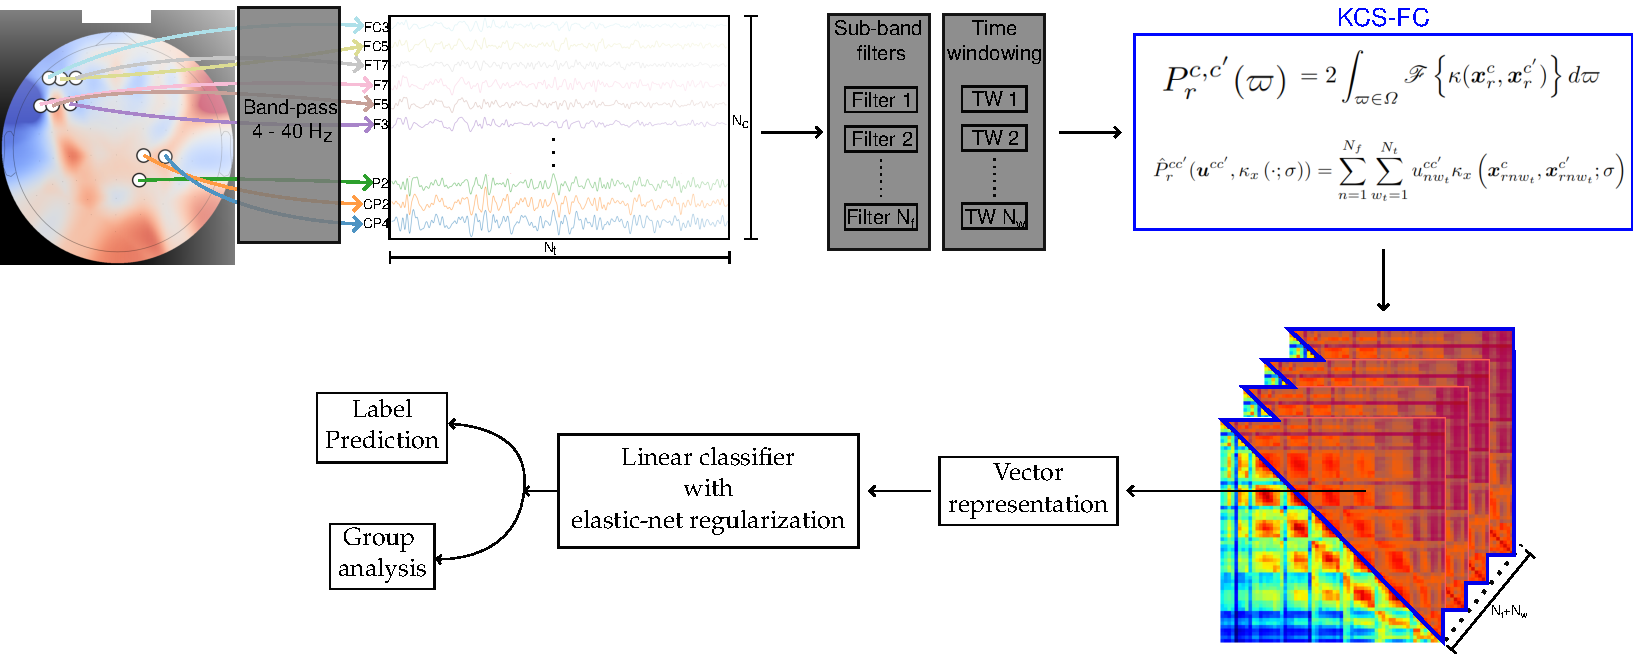
\includegraphics[scale=0.6]{Figures/outline_and_contributions/contribution1_C.pdf}
    \caption{Illustration of the proposed Kernel-based Cross-Spectral FC for enhancing the MI-BCI model's accuracy. Key features include robust FC estimators using a Gaussian kernel for non-linearity, short sliding windows for addressing non-stationarity, sub-band filtering for managing inter-subject variability, vectorization representation for FC extraction and elastic-net regularization to curb spurious connectivities \label{fig:contribution1}}
\end{figure}

\section{Kernel-based Covariance Function}
\changes{The Wiener-Khinchin's theorem states that a real-valued auto-correlation function, $R^{c}_{r}(\tau)$, of a weak-sense stationary stochastic process $x^{c}_{r}(\tau)$ can be defined as~\cite{cohen1998generalization}:
\begin{equation}\label{eq:wiener}
	R^{c}_{r}(\tau) = \int_{\varpi \in \Omega}\exp({j2\pi \tau \varpi})dP^{c}_{r}(\varpi) ,
\end{equation}
where $P^{c}_{r}(\varpi)\en\Real[0,1]$ is a monotonic spectral distribution function absolutely continuous and differentiable over frequency $\varpi \in \Omega$.
According to Bochner's theorem the univariable relationship in~Equation~\eqref{eq:wiener} a stationary positive-definite kernel \changes{$\kappa^{cc'}_{r}(\Delta_{x}) = \kappa(\ve{x}^{c}_{r},\ve{x}^{c'}_{r})$} can be related with its cross-spectral counterpart $S^{cc'}_{r}(\varpi)$ if and only if the following assumption holds between both spectral representations~\cite{bochner2020harmonic}:
\begin{equation}\label{eq:kCSD}
	\kappa^{cc'}_{r}(\Delta_{x}) = \int_{\varpi \in \Omega} \exp{(j2\pi {\Delta_{x}} \varpi)} S^{cc'}_{r}(\varpi)d\varpi,
\end{equation}
where $\Delta_{x} = \ve{x}^{c}_{r} - \ve{x}^{c'}_{r}$ is the vector delay, $\varpi\subseteq\varOmega$ is the frequency domain that contains the bandwidth set of analysis $\varOmega$, and $ S^{cc'}_{r}(\varpi)$ is the cross-spectral density that preserves the following equality: $ S^{cc'}_{r}(\varpi) = d {P}^{cc'}_{r}(\varpi)/d\varpi$, with $ P^{cc'}_{r}(\varpi)\en\Real[0,1]$ being the cross-spectral distribution that is related to the mapping kernel, $\kappa: \Real^{N_t} \times \Real^{N_t}\to \Real$.
As regards $\kappa(\ve{x}^{c}_{r},\ve{x}^{c'}_{r}) = \langle \phi(\ve{x}^{c}_{r}),\phi(\ve{x}^{c'}_{r}) \rangle_{\mathcal{H}}$, it is a positive-definite stationary kernel inducing the nonlinear feature mapping $\phi(\cdot)$ to a Reproducing Kernel Hilbert Space, $\mathcal{H}$. Notation $\langle \cdot,\cdot \rangle$ represents the dot product. 
Therefore, we compute the cross-spectral distribution $ P^{cc'}_{r}(\varpi)$ within a bandwidth $\varOmega$, as below:
\begin{equation}
	\begin{aligned}\label{eq:CSDist}
		P^{cc'}_{r}(\varpi) &= 2\int_{\varpi \in \varOmega} S^{cc'}_{r}(\varpi)d\varpi,\\
		&=2\int_{\varpi \in \varOmega} \mathscr{F}\left\{\kappa(\ve{x}^{c}_{r},\ve{x}^{c'}_{r}) \right\}d\varpi,
	\end{aligned}
\end{equation}
where notation $\mathscr{F}\{\cdot\}$ stands for the Fourier transform. 
}

As a result,~Equation~\eqref{eq:CSDist} preserves the frequency-based interpretation of the kernel-based pairwise dependencies that were estimated between vectors of random functions. Furthermore, the imposed stationary kernel favors the extraction of nonlinear data dependencies~\cite{bishop2006pattern}

\section{Gaussian Functional Connectivity from Kernel-based Spectral Distribution}
\changes{
Let $\ve{x}^{c}_{rnw_t}$ be an EEG channel $c$ at trial $r$ within filter $n$ and time window $w_t$, and $\{ \ve{x}^{c}_{rnw_t} \in \Real^{N_t}, {y}_r \in \Real[0,1]\}_{c,r,n,w_t=1}^{N_c,R,N_f,N_t}$ be an time segmented filtered EEG set holding all channels $N_c$, $R$ trials, $N_f$ frequency bandwidths, $N_t$ time windows , ${y}_r$ is the class or label assigned to the $r$-th trial, and the notation $|\cdot|$ stands for set cardinality. Since the Gaussian kernel is preferred in pattern classification because of its universal approximating ability and mathematical tractability~\cite{Alvarez-Meza2014}, we propose the Gaussian function to compute the pairwise kernel-based dependencies between channels $c$ and $c'$, without the case $c\neq c'$ in~Equation~\eqref{eq:kCSD}, termed Gaussian Functional Connectivity (KCS-FC), defined as follows:
\begin{equation}
		\kappa_x\left(\ve{x}^{c}_{rnw_t}, \ve{x}^{c'}_{rnw_t};\sigma\right) = \exp{\left( {-\|\ve{x}^{c}_{rnw_t}-\ve{x}^{c'}_{rnw_t}\|^2_2}/{2\sigma^2}\right)}, \label{eq:gkernel}
\end{equation}
where $\sigma\en\Real^+$ is the length scale hyperparameter. Notation $\|\cdot\|_q$ stands for $\ell_q$-norm.
}

With the aim to implement the single-trial extraction, \changes{we estimate the cross-spectral distribution $\hat{\mat{P}}^{cc'}_{r}$ between a pair of channels $c$ and $c'$ at trial $r$ as follows:}
\changes{
\begin{equation}\label{eq:fcc}
	\hat{P}^{cc'}_{r}(\ve{u}^{cc'},\kappa_x\left(\cdot;\sigma\right)) = \sum_{n=1}^{N_f}\sum_{w_t=1}^{N_t} u_{nw_t}^{cc'}\kappa_x\left(\ve{x}^{c}_{rnw_t},\ve{x}^{c'}_{rnw_t};\sigma\right),
\end{equation}
where $\ve{u}^{cc'} \in \Real^{N_f N_t}$ is the spatio-temporal-frequency (\textit{s-t-f}) relevance vector that codes the pairwise undirected dependency between channels and contains the values $u_{nw_t}^{cc'}$ holding the relevance value estimated at $n$-th frequency and $w_t$ window.
}

\changes{Using the single-trial kernel-based spectral distribution representation in~Equation~\eqref{eq:fcc}, we propose extracting the sparse functional connectivity, using the Elastic Net regularization \cite{tay2023elastic}, aiming to finding discriminative and interpretable brain activity patterns.
\begin{equation}\label{eq:SRC}
	\ve{u}^* = \arg \min_{\ve{u}} \promed{ \sum_{r=1}^{R} \left\|\sum_{c,c'=1}^{N_c}\hat{P}^{cc'}_{r}(\ve{u}^{cc'},\kappa_x(\cdot;\sigma))-y_r\right\|^2_2} + \alpha \sum_{c,c'=1}^{N_c}\|\ve{u}^{cc'}\|_1 + \frac{1-\alpha}{2} \sum_{c,c'=1}^{N_c}\|\ve{u}^{cc'}\|_2 \quad :  \forall c < c',
\end{equation}
where $\alpha \in \Real^+$ is the regularization hyperparameters, and $\| \cdot \|_q$ is the $\ell_q$-norm.
}

\changes{Without loss of generallity, equation~\eqref{eq:SRC} can be rewritten as:
\begin{equation}
	\ve{\tilde{u}}^* = \arg \min_{\ve{\tilde{u}}} \promed{\sum_{r=1}^{R} \|\ve{\tilde{u}}\ve{\tilde{p}_{r}}^{\top}-y_r\|^2_2} + \alpha \|\ve{\tilde{u}}\|_1 + \frac{1-\alpha}{2} \|\ve{\tilde{u}}\|_2, \label{eq:SRC_vec}
\end{equation}
where $\top$ is the vector transpose, $\ve{\tilde{u}}$ and $\ve{\tilde{\kappa}}$ stand for the spatio-temporal-frequency relevance matrix and cross-spectral distribution vector concatenation obtained as:
\begin{equation}
	\begin{aligned}
		\ve{\tilde{u}} &= \left[u_{11}^{12},u_{11}^{13},\cdots,u_{11}^{1N_c},u_{11}^{23},\cdots,u_{11}^{(N_c-1)N_c},u_{12}^{12},\cdots, u_{N_fN_t}^{(N_c-1)N_c} \right], \\
		\ve{\tilde{p}}_{r} &= \left[ \hat{P}_{r11}^{12},\hat{P}_{r11}^{13},\cdots,\hat{P}_{r11}^{1N_c},\hat{P}_{r11}^{23},\cdots,\hat{P}_{r11}^{(N_c-1)N_c},\hat{P}_{r12}^{12},\cdots, \hat{P}_{rN_fN_t}^{(N_c-1)N_c} \right] ,\\
	\end{aligned}
\end{equation}
Note that for simplicity the term $\hat{P}^{cc'}_{r}(\mat{U}^{cc'}_{r},\kappa_x\left(\cdot;\sigma\right))$ is rewritten as $\hat{P}^{cc'}_{rnw_t}$.
}

Consequently, the optimization framework in~Equation~\eqref{eq:SRC_vec} allows for computing the spectral combination weights from the extracted filter-bank representations that match the MI class-probability set, resulting in a sparse, relevant kernel-based functional connectivity between pairs of EEG channels.


\section{Experimental Set-Up}
The evaluation of the considered functional connectivity measures for enhanced feature extraction is performed according to the following stages: 

\changes{
({i}) Preprocessing and trial-based extraction of {s-t-f} representations. For extracting the subject EEG dynamics over time accurately, the sliding window length of feature extraction is fixed to the next values: $\tau=[0.5,1.0,1.5,2.0]$\,{s}, having an overlap of $75\%$. Additionally, similar to authors in \cite{ang2008filter} the frequency bands of interest are selected with the lower frequency limit set at 4 Hz, the upper limit set to 40 Hz, and an overlap of $50\%$.
}

\changes{
({ii}) The estimation of the single-trial functional connectivity from the extracted {s-t-f} features. For comparison, the proposed KCS-FC is contrasted with two commonly used single-trial FC measures. To facilitate this comparison, the KCS-FC in Equation~\eqref{eq:SRC} is interchanged with new single-trial FC measures. These measures can be estimated from a frequency $n$, a time window $w_t$, and a pair of channels ${cc'}$ (with $c \neq c'$, for all $cc'$ in $C$) as described in~\cite{rodrigue2019}.
\begin{equation}
			\rho(\ve{x}^{c}_{rnw_t},\ve{x}^{c'}_{rnw_t}) ={\left<\ve{x}^{c}_{rnw_t},\ve{x}^{c'}_{rnw_t}\right>}\label{Eq:Pearson}
\end{equation}
\begin{equation}		 
	{\Delta\phi(\ve{x}^{c}_{rnw_t},\ve{x}^{c}_{rnw_t})}  {= {|\exp(j(\ve{\phi}_{rnw_t}^{c}-\ve{\phi}_{rnw_t}^{c}))|}} \label{Eq:PLV} 
\end{equation}
}
where $\ve{x}^{c}_{rnw_t}$ and $\ve{x}^{c'}_{rnw_t}$ is the real-valued EEG data from the corresponding electrodes at trial $r$ (within temporal window $w_t$ and frequency band $n$) with instantaneous phases $\ve{\phi}_n^{ct}$ and $\ve{\phi}_n^{c't}$, respectively. The pairwise relationships in~Equations~\eqref{Eq:Pearson} and~\eqref{Eq:PLV} are referred as {Cross-Correlation Coefficient}(CCF) and {Phase Lag Value} (PLV), respectively.

{For feeding the classifier procedure, we evaluate two feature representation approaches that are extracted from each tested FC measure: Firstly, the feature representation is the CSP's pattern vector (linear projection of the sample covariance), computed as detailed in~\cite{velasquez2020dynamic}; in particular, the well-known CSP's eigendecomposition is applied by replacing the covariance matrix with the corresponding FC measure. Secondly,  the concatenated (vectorized) triangular representation of the symmetrical FC matrices is extracted, as detailed in~\cite{barachant2013classification}. Both of the approaches comprise a filter-bank-based concatenation strategy through a fixed sliding window size and overlap values; that is, the temporal dependencies between windows are not directly modeled.}

({iii}) Sparse feature selection and classifier performance computation. {Here, for implementation purposes, the optimizing problem is solved through the well-known Elastic-net algorithm to deal appropriately with redundant information. It is worth noting that we prefer Elastic-net over the Lasso-based regularization, because, when the number of features is greater than the number of training samples, Lasso behaves erratically~\cite{geron2022hands}.}

For comparative purposes, we also perform feature extraction using the baseline CSP-based spatial filtering that is widely used for filtering measures of synchronization~\cite{haddad2019early,kumar2018eeg}. To this end, we perform the CSP feature extraction, adjusting the sliding time window length at each evaluated value of $\tau$ and fixing the variance of the surrogate space to the first three eigenvectors of the spatial filtering matrix, as suggested in~\cite{lotte2018review}. It is worth mentioning that we evaluate the FC measures in~Equations~\eqref{Eq:Pearson} and \eqref{Eq:PLV}, as well the CSP-based feature extraction scheme, through the sparse model presented in~Equation~\eqref{eq:SRC} using a vector concatenation approach through temporal windows and frequency bands.

({iv}) Clustering of subject inefficiency and interpretation analysis. 
For enhancing the interpretive analysis, we cluster the differences in neural responses that depend on the users' motor skills. The intra/inter-subject variability affects the FC estimators' robustness properties, becoming stronger for the worst-performing individuals.

{Regarding the performance measure, the classifier accuracy $a_c\en[0,1]$ is computed, as follows:
$$a_c= \,(T_P \s{~+~} T_N )/ (T_P\s{~+~} T_N \s{~+~} F_P \s{~+~} F_N ),$$
 where $T_P$, $T_N$, $F_P$, and $F_N$ are true-positives, true-negatives, false-positives, and false-negatives, respectively. A stratified $10$-fold cross-validation strategy randomly partitions the training and testing sets.}

\section{Results and Discussion}

\subsection{Influencing FC Parameters on Accuracy Estimation}

\subsubsection{Impact of Prior CSP Filtering}

{\changes{For} interpretation purposes, Figure \ref{Fig:FCx} presents the subjects' accuracy in decreasing order by all evaluated EEG data collections. Each data set is tested in two configurations to feed the sparse feature selector: using feature concatenation (odd rows) and linearly mapping through CSP (even rows). The FC measures' accuracy is estimated at each $\tau$ ({PLV}---left column, {CCF}---middle column, {KCS-FC}---right column), adjusting the parameter $\sigma$ to the median averaged over the input distances for kernel-based functional connectivity computation.} 

{The top plots display the results that were performed by the databases with a similar amount of subjects: DMBI MI (first and second rows) and DB DBII ME (third and fourth rows). As seen, PLV yields the most scattered outcomes, with a significant portion accomplishing low accuracy.} {A similar situation holds for DBIII MI with a more visible subject variability: PLV discriminates the worst, followed by CCF, and KCS-FC performs a bit better, still outperforming the other FC when compared and having the accuracy values less spread throughout the subject set}. However, the accuracy estimates are significantly more dispersed across the individuals than in DBII ME, regardless of the FC measure. Several factors may account for the higher variability of MI data. The EEG montage of MI protocols is more complex ($64$ MI channels vs. $44$ ME channels). Besides, the ME signals are reported as having a higher degree of regularity than MI practicing, at least in terms of motor-related discriminability~\cite{shamsi2020early}. Consequently, even if the DBIII MI collection doubles the number of trials compared with DBII ME, the subject variability of MI data remains high enough to limit the CSP effectiveness (see the bottom row). Moreover, numerous subjects achieve accuracy values that are below $60\%$, which is, under the BCI-inefficiency level reported~\cite{Sanelli2019}. 

\subsubsection{Influence of Sliding Windows}

\Cref{Fig:AccTau} summarizes \changes{impact of the sliding window's length} on the classifier discrimination ability using each evaluated measure of FC. In the case of DBI MI, the first row shows that PLV and CCF both obtain very close performance if the CSP filtering is not involved at all tested window values. Otherwise, the latter measure notably improves in performance. Nevertheless, the proposed KCS-FC outperforms, and this behavior remains valid in the second row that presents the accuracy of DBII ME with more subject variability, as shown by the average bars. However, some fluctuations in the PLV and CCF performance are more evident after applying CSP, depending on the window. Instead, the KCS-FC measure presents performance nearly invariant across the range of considered sliding window lengths, being slightly enhanced by the CSP filtering algorithm.

\changes{Additionally}, the bottom row presents the classifier performance that is obtained by MI activity (DBIII MI) with the most challenging subject variability, showing that the accuracy of all FC measures drops, particularly in the case of PLV. As seen, the PLV and CCF accuracy values are more sensitive to the sliding window influence, while the proposed KCS-FC assessments remain constant over the range of $\tau$. One more aspect to highlight is that the CSP-based filtering effectiveness becomes more dependent on the specific sliding window selected. Furthermore, under increased subject variability, this spatial filtering method's application noticeably decreases the KCS-FC performance.

\subsection{Estimated Classifier Accuracy of Individuals}

The following consideration is linked to the quality of individual FC assessments because of their diverse variability. For this purpose, Figure \ref{Fig:IndividualAcc} illustrates the individual classifier performance at each window length, for which the subjects are displayed on the horizontal axis in decreasing order of the CCF accuracy achieved at $\tau=2$\,{s} (the continuous line outlined in blue color). The rationale for choosing this specific FC estimation case as the baseline is that the cross-correlation coefficient that is presented in~Equation~\eqref{Eq:Pearson} can be directly associated with the conventional Pearson estimate with the simplest interpretation regarding pairwise relationships~\cite{georgiadis2019connectivity}.

\def \kerrwidth {.2\linewidth}
\begin{figure}[h!]
\centering
	\hbox{\hspace{4.5cm} {PLV}\hspace{2.6cm} {CCF}\hspace{2.7cm} {KCS-FC}}
	\rotatebox{90}{ \quad\, \textbf{\tiny DBI MI}}
	\rotatebox{90}{\quad\,\tiny{Accuracy ($\%$)}}
	{\resizebox{\kerrwidth}{!}{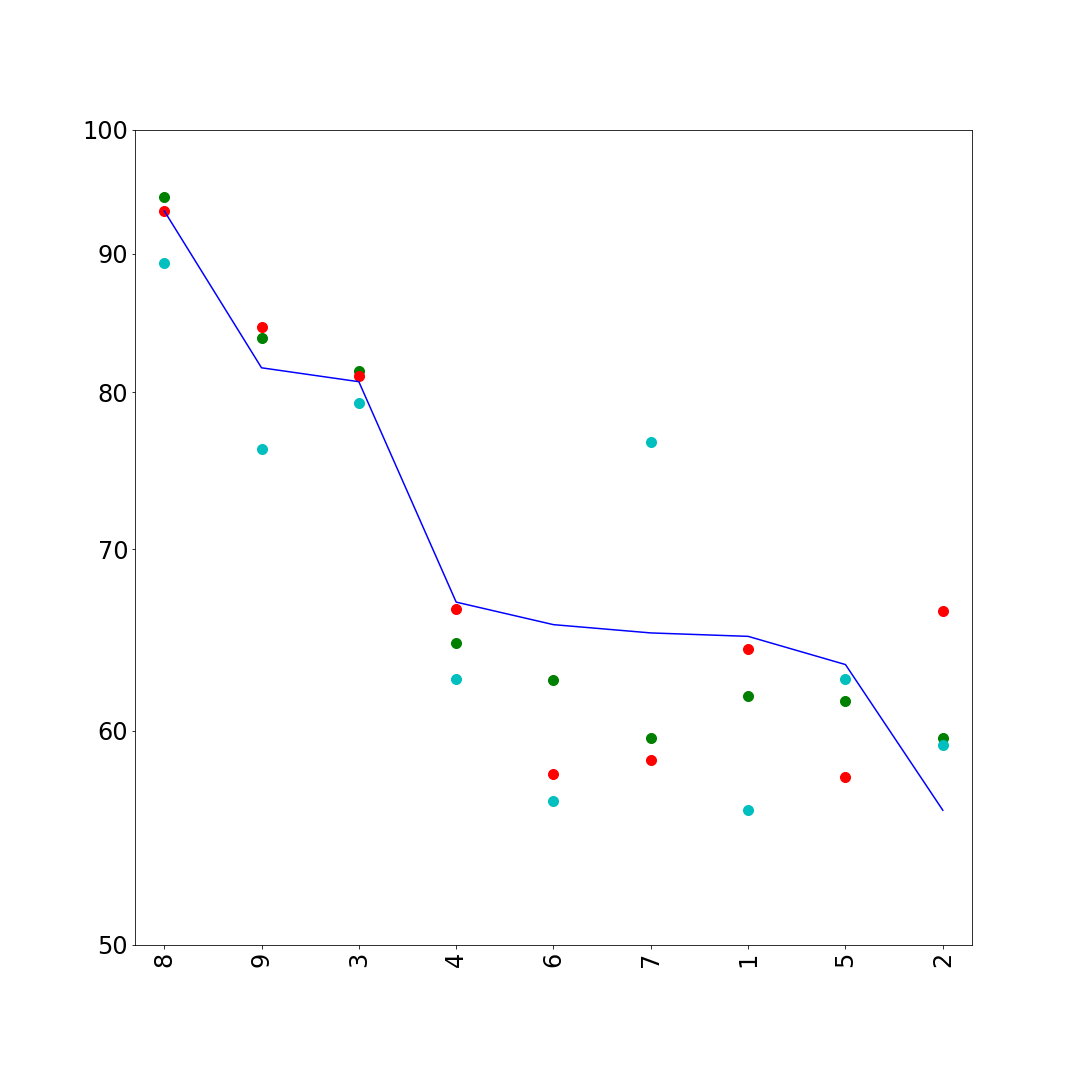
\includegraphics[trim=85 100 80 80, clip]{Figures/Objective_1/taus_plv_BCI_MI.png}}}
	{\resizebox{\kerrwidth}{!}{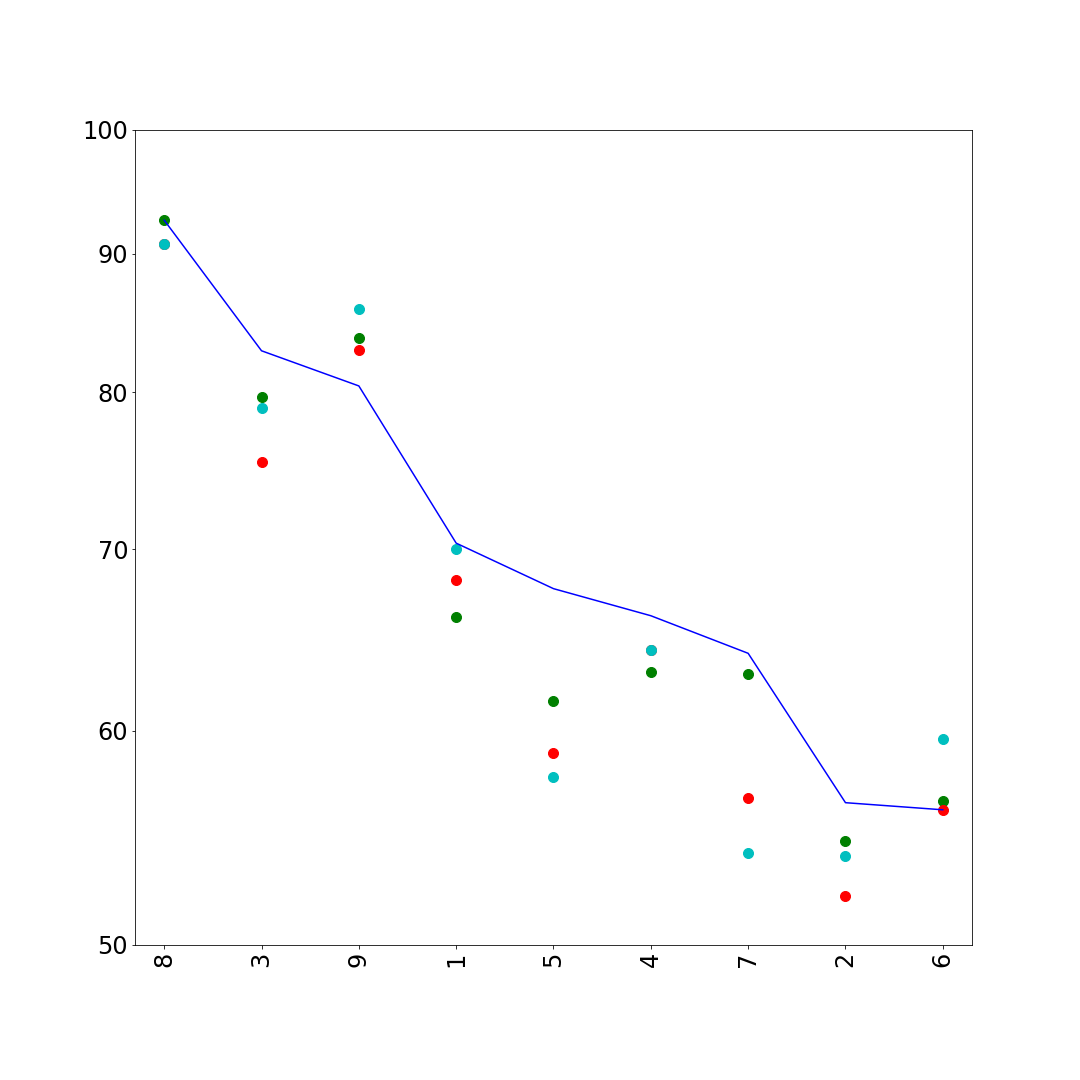
\includegraphics[trim=85 100 80 80, clip]{Figures/Objective_1/taus_pearson_BCI_MI.png}}}
	{\resizebox{\kerrwidth}{!}{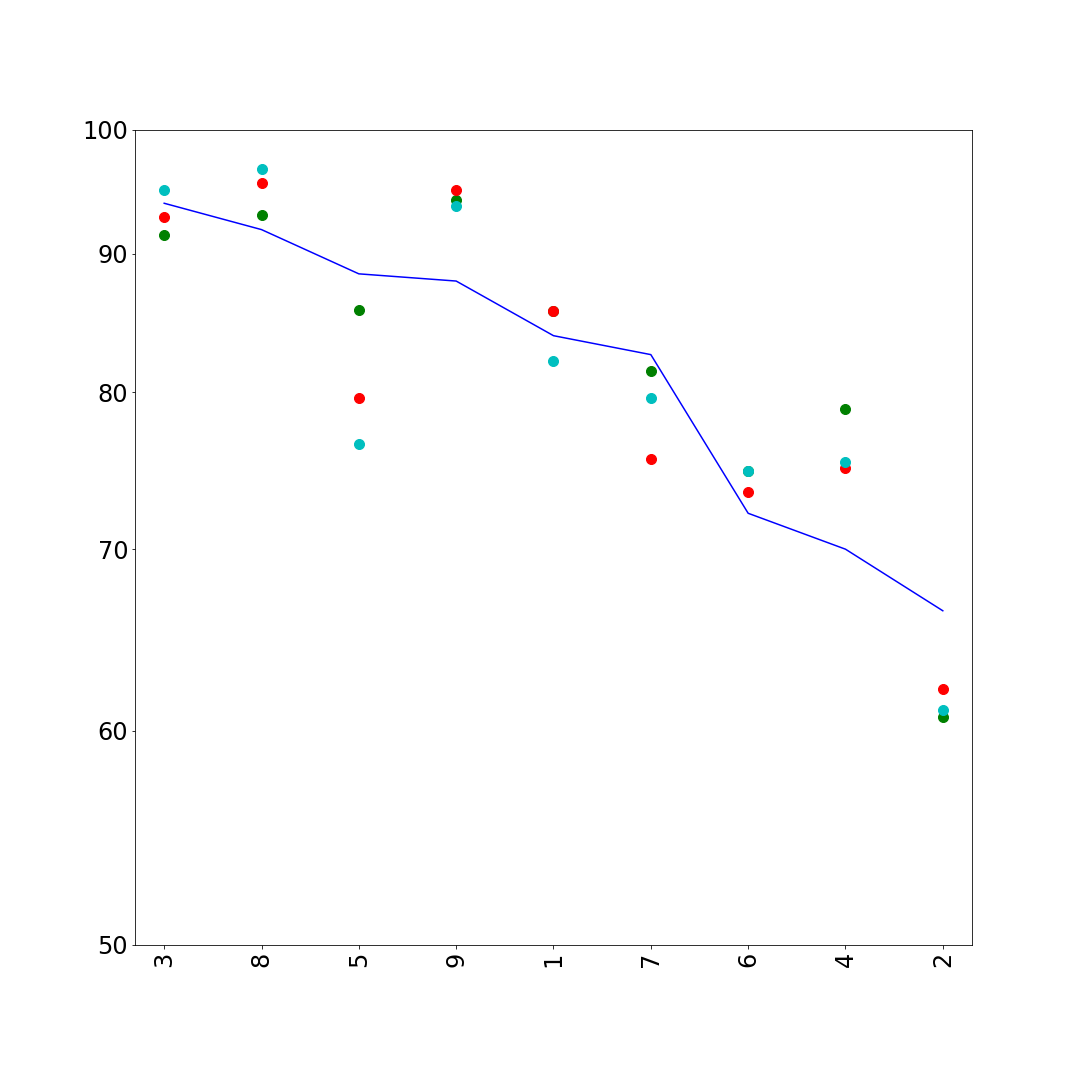
\includegraphics[trim=85 100 80 80, clip]{Figures/Objective_1/taus_gauss_BCI_MI.png}}}\\	
	\rotatebox{90}{ \quad\, \textbf{\tiny DBI MI-CSP} }
	\rotatebox{90}{\quad\,\tiny{Accuracy ($\%$)}}
	{\resizebox{\kerrwidth}{!}{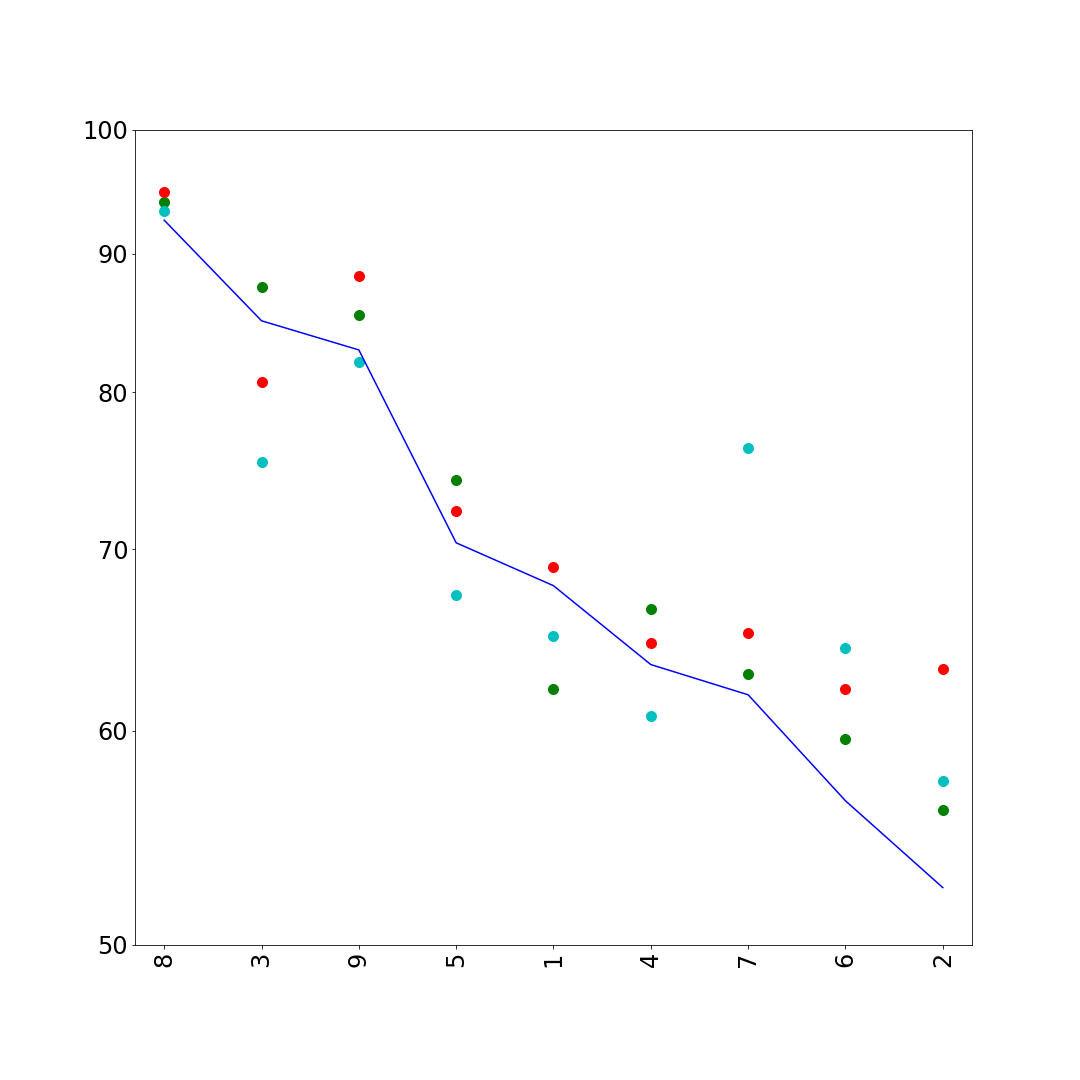
\includegraphics[trim=85 100 80 80, clip]{Figures/Objective_1/taus_csp_plv_BCI_MI.png}}}
	{\resizebox{\kerrwidth}{!}{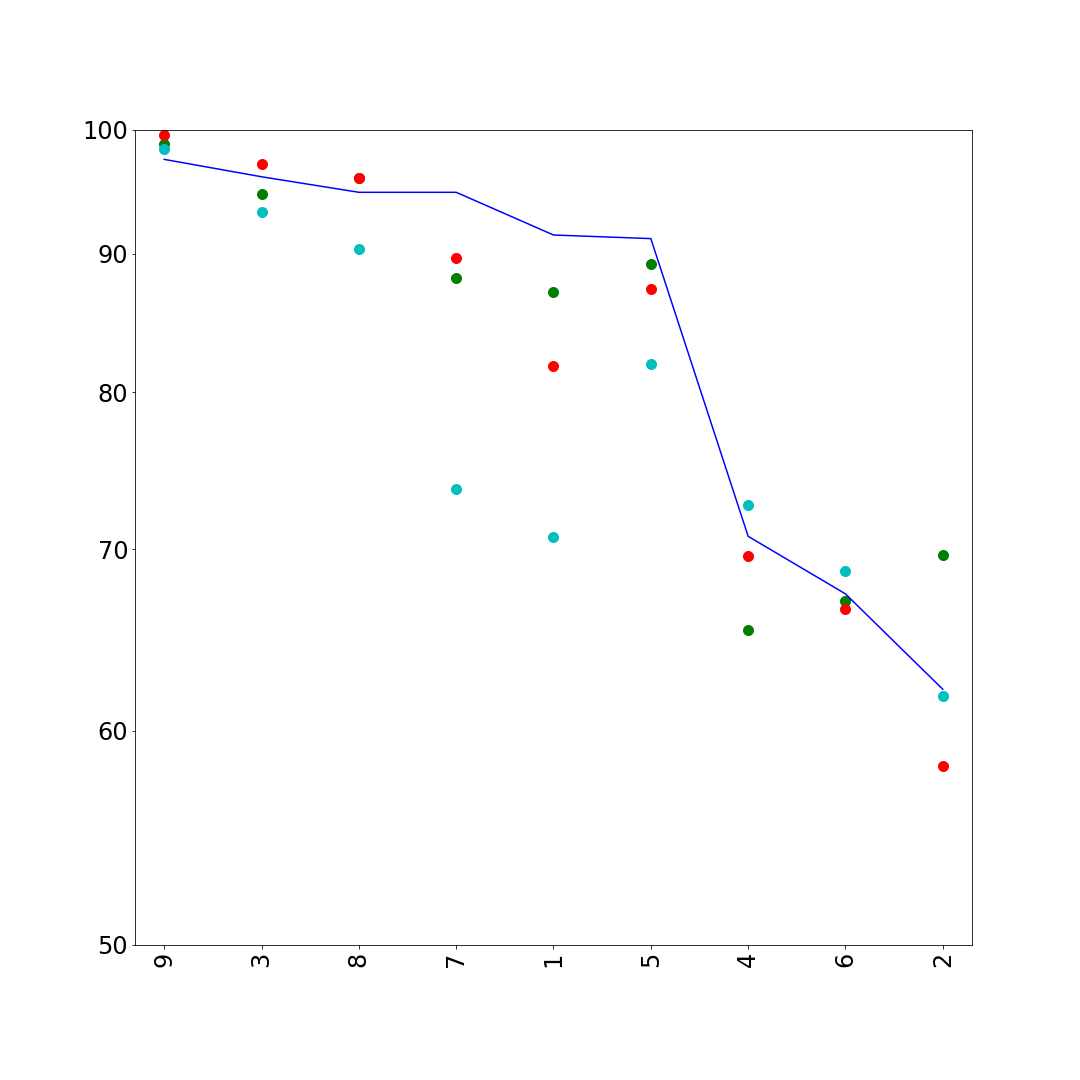
\includegraphics[trim=85 100 80 80, clip]{Figures/Objective_1/taus_csp_pearson_BCI_MI.png}}}
	{\resizebox{\kerrwidth}{!}{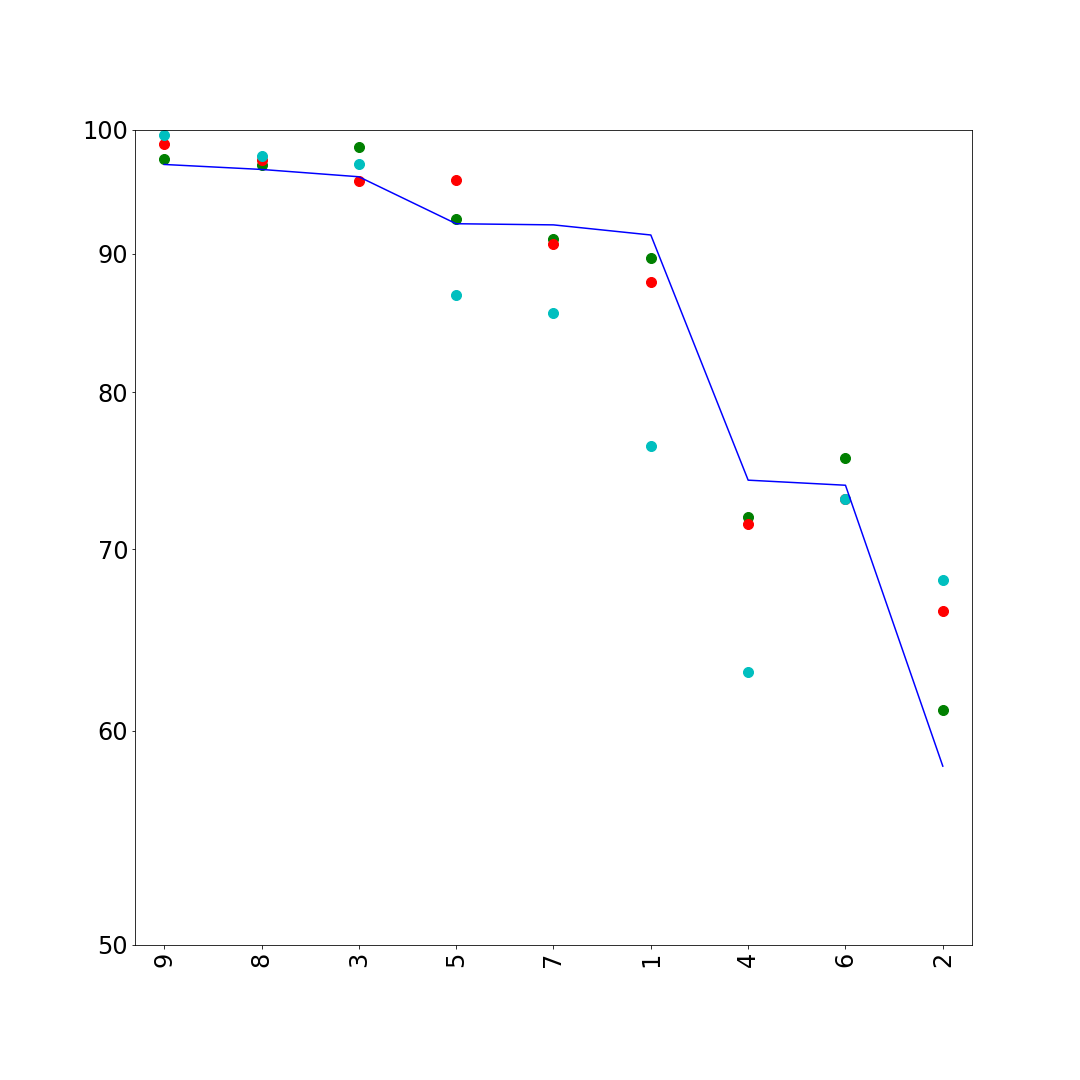
\includegraphics[trim=85 100 80 80, clip]{Figures/Objective_1/taus_csp_gauss_BCI_MI.png}}}\\	
	\rotatebox{90}{ \quad\, \textbf{\tiny DBII ME}}
	\rotatebox{90}{\quad\,\tiny{Accuracy ($\%$)}}
	{\resizebox{\kerrwidth}{!}{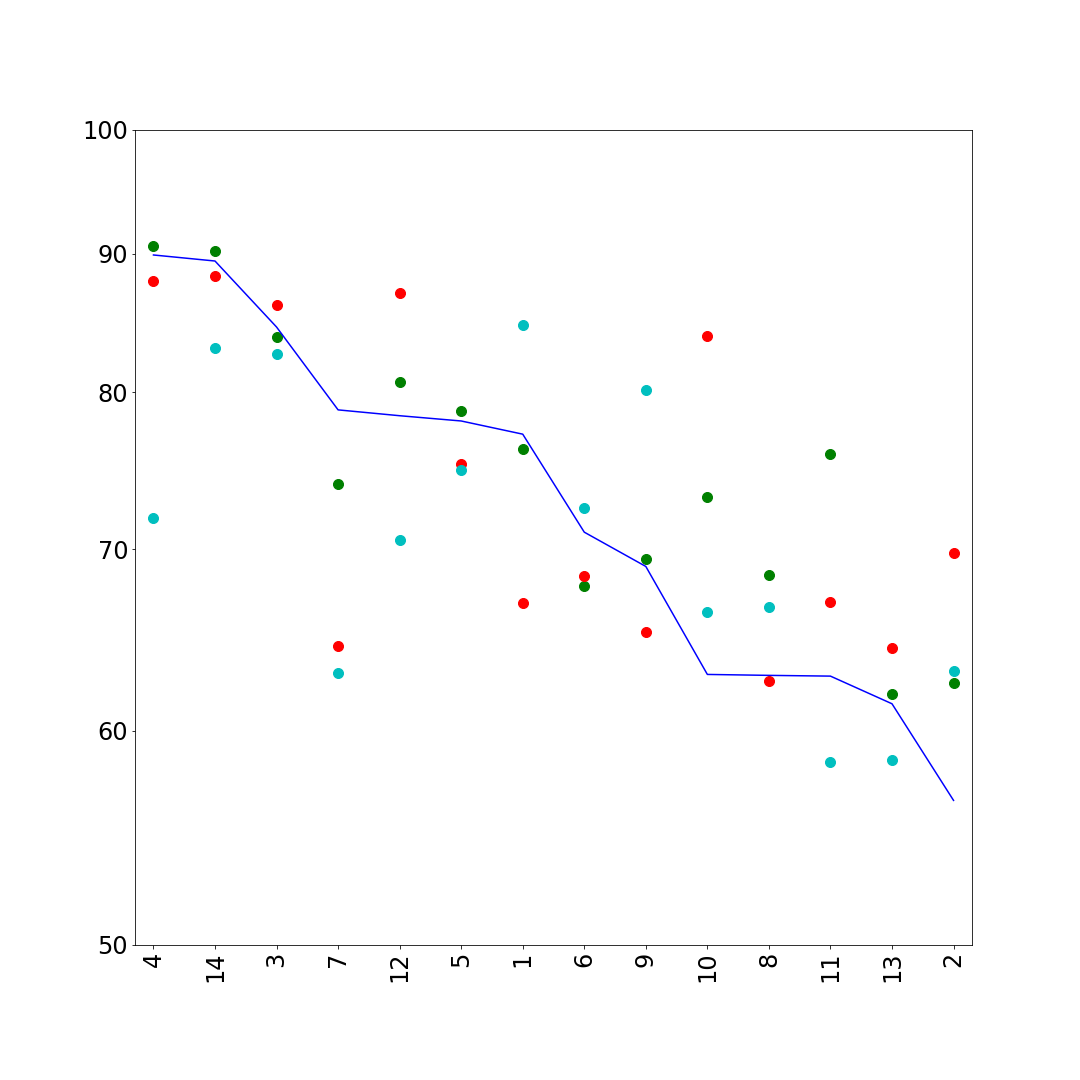
\includegraphics[trim=85 100 80 80, clip]{Figures/Objective_1/taus_plv_HG_ME.png}}}
	{\resizebox{\kerrwidth}{!}{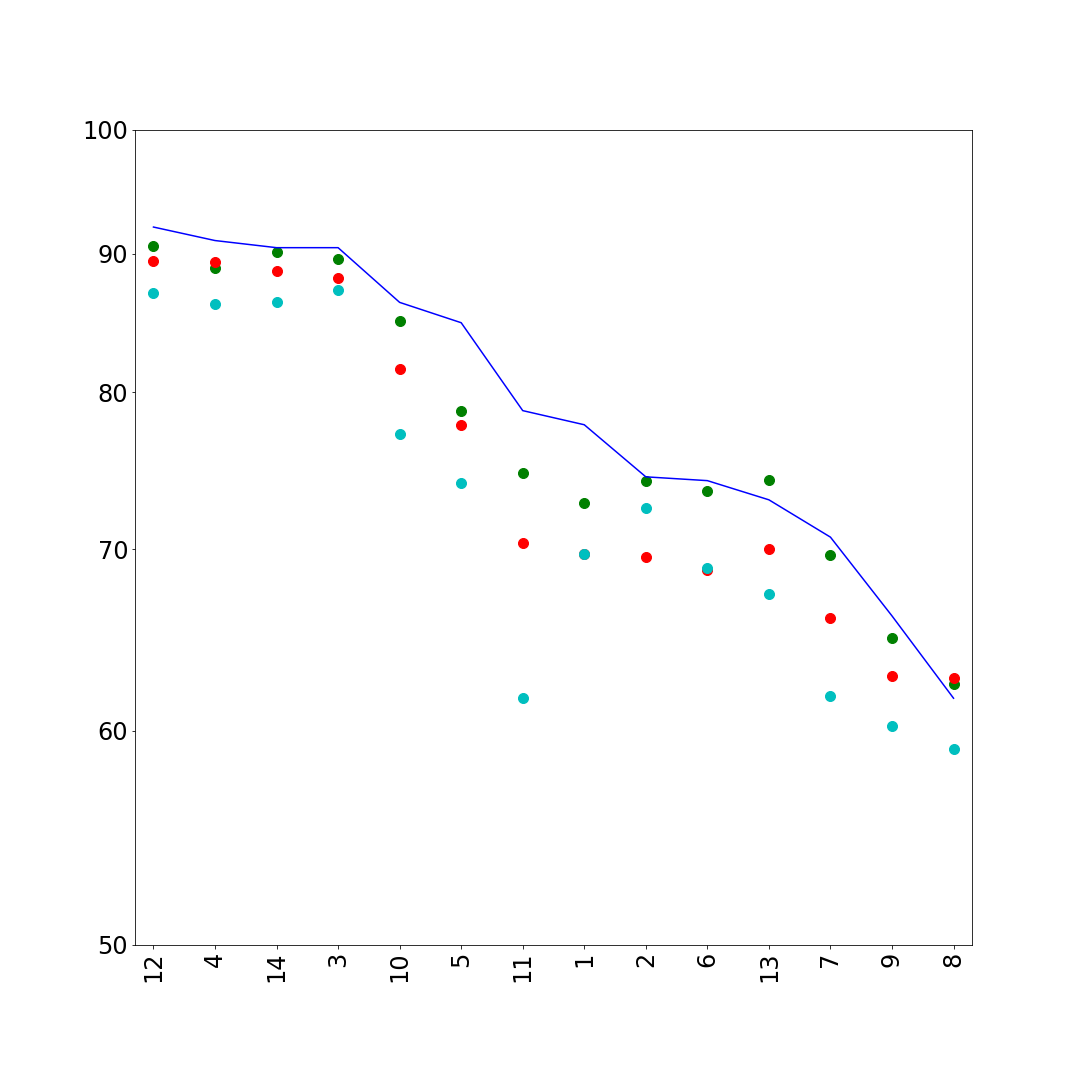
\includegraphics[trim=85 100 80 80, clip]{Figures/Objective_1/taus_pearson_HG_ME.png}}}
	{\resizebox{\kerrwidth}{!}{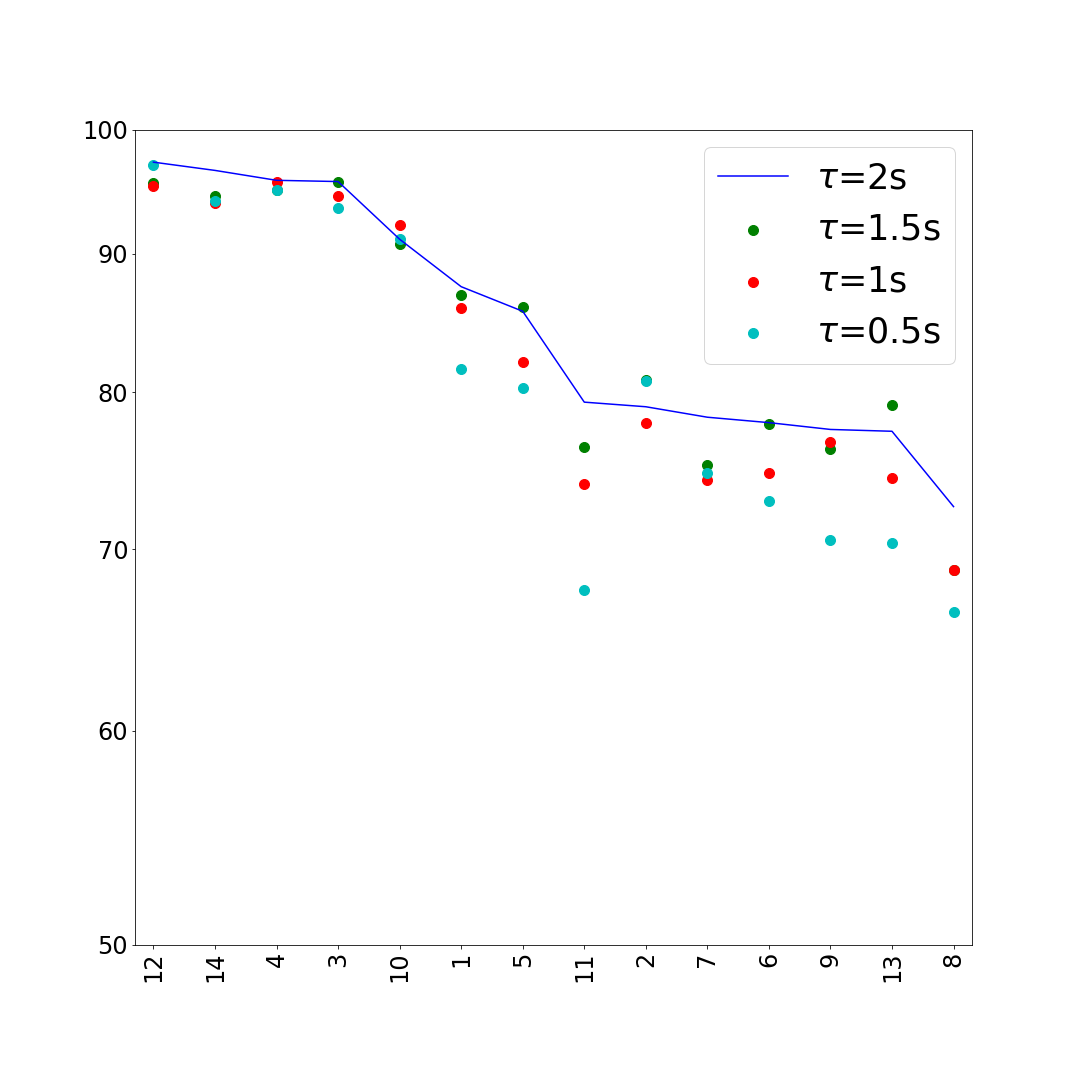
\includegraphics[trim=85 100 80 80, clip]{Figures/Objective_1/taus_gauss_HG_ME.png}}}\\
	\rotatebox{90}{ \quad\, \textbf{\tiny DBII ME-CSP}}
	\rotatebox{90}{ \quad\,\tiny{Accuracy ($\%$)}}
	{\resizebox{\kerrwidth}{!}{\includegraphics[trim=85 100 80 80, clip]{Figures/Objective_1/taus_CSP_plv_HG_ME.png}}}
	{\resizebox{\kerrwidth}{!}{\includegraphics[trim=85 100 80 80, clip]{Figures/Objective_1/taus_CSP_pearson_HG_ME.png}}}
	{\resizebox{\kerrwidth}{!}{\includegraphics[trim=85 100 80 80, clip]{Figures/Objective_1/taus_CSP_gauss_HG_ME.png}}}\\
	\rotatebox{90}{ \quad\, \textbf{\tiny DBIII MI}}
	\rotatebox{90}{ \quad\,\tiny{Accuracy ($\%$)}}
	{\resizebox{\kerrwidth}{!}{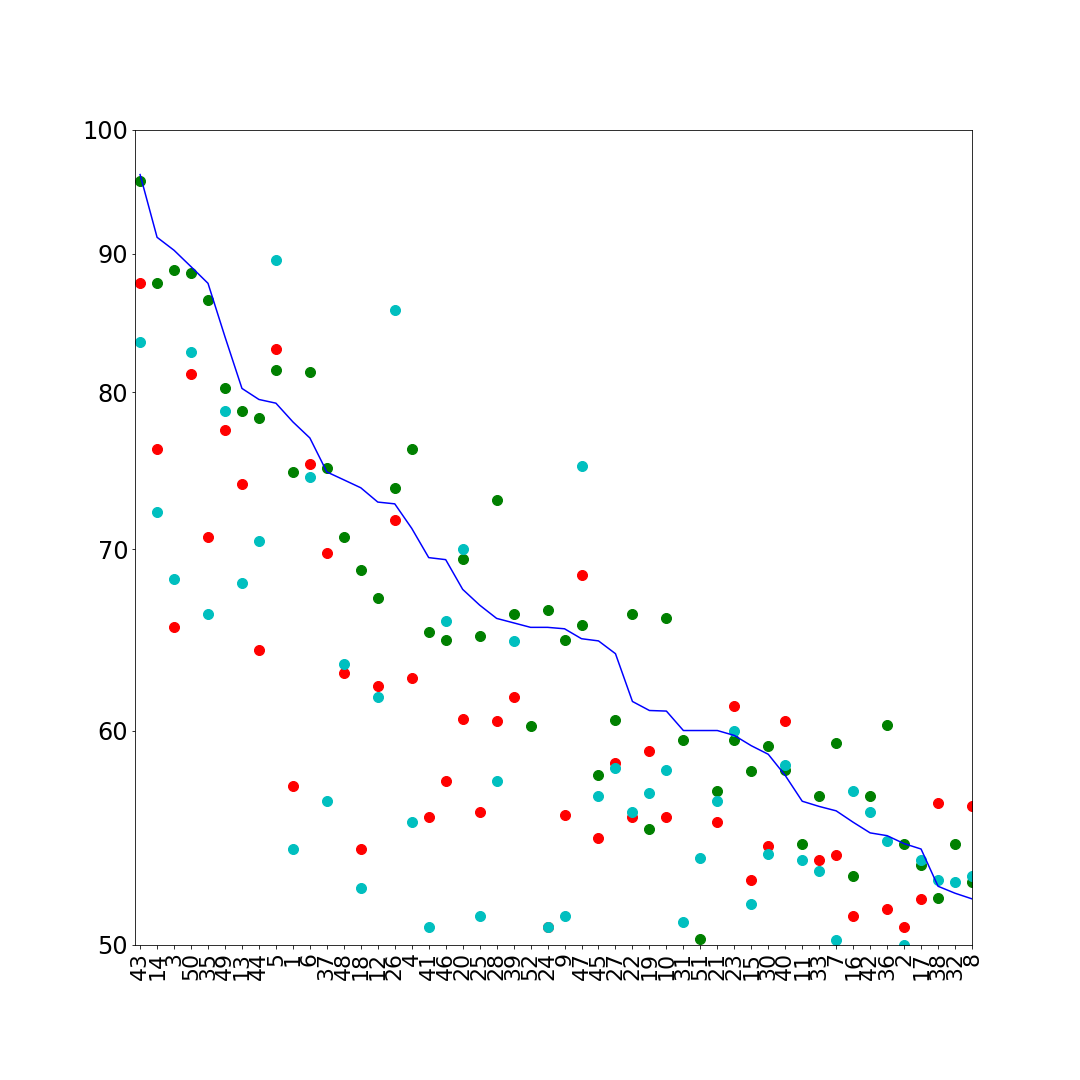
\includegraphics[trim=85 100 80 80, clip]{Figures/Objective_1/taus_plv_giga_MI.png}}}
	{\resizebox{\kerrwidth}{!}{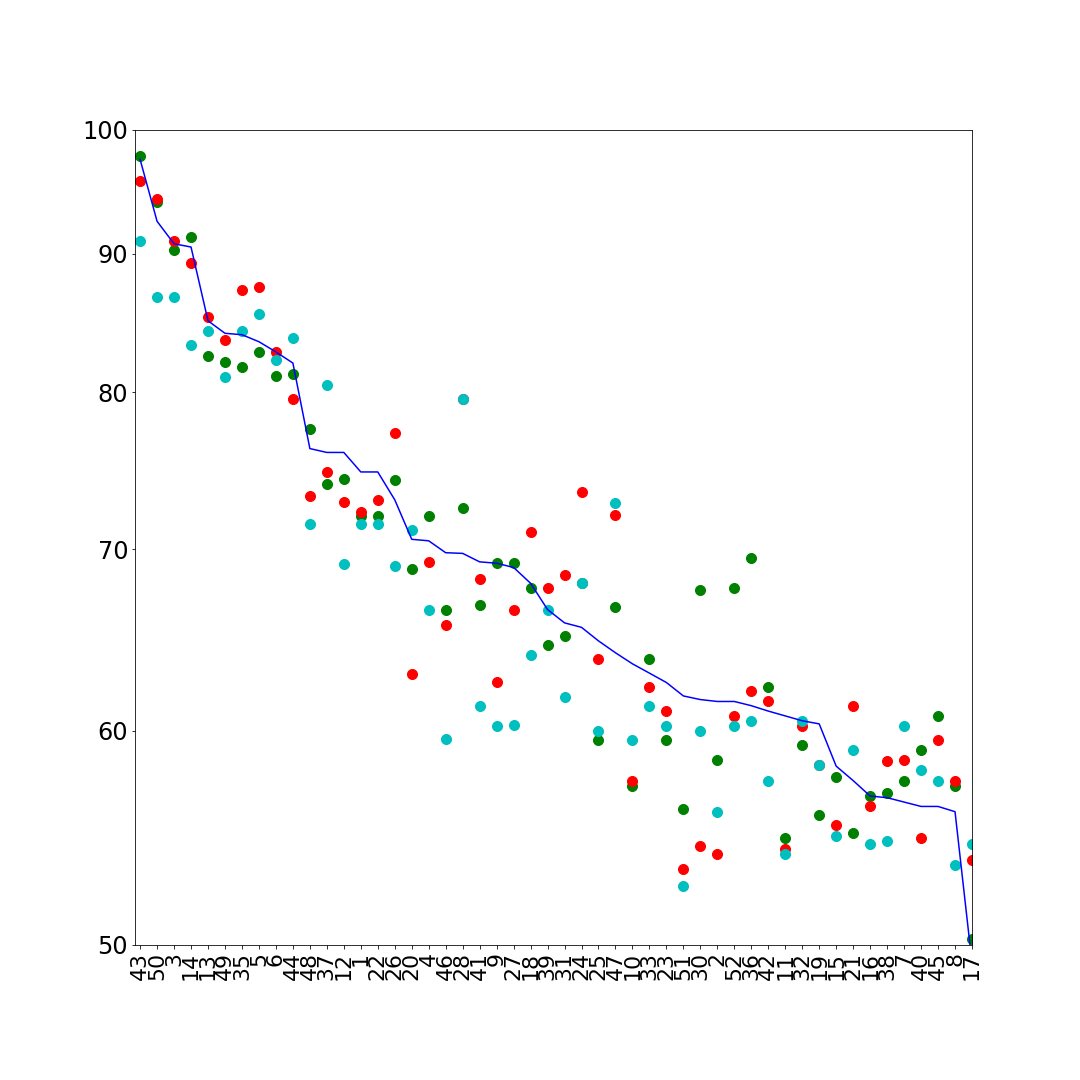
\includegraphics[trim=85 100 80 80, clip]{Figures/Objective_1/taus_pearson_giga_MI.png}}}
	{\resizebox{\kerrwidth}{!}{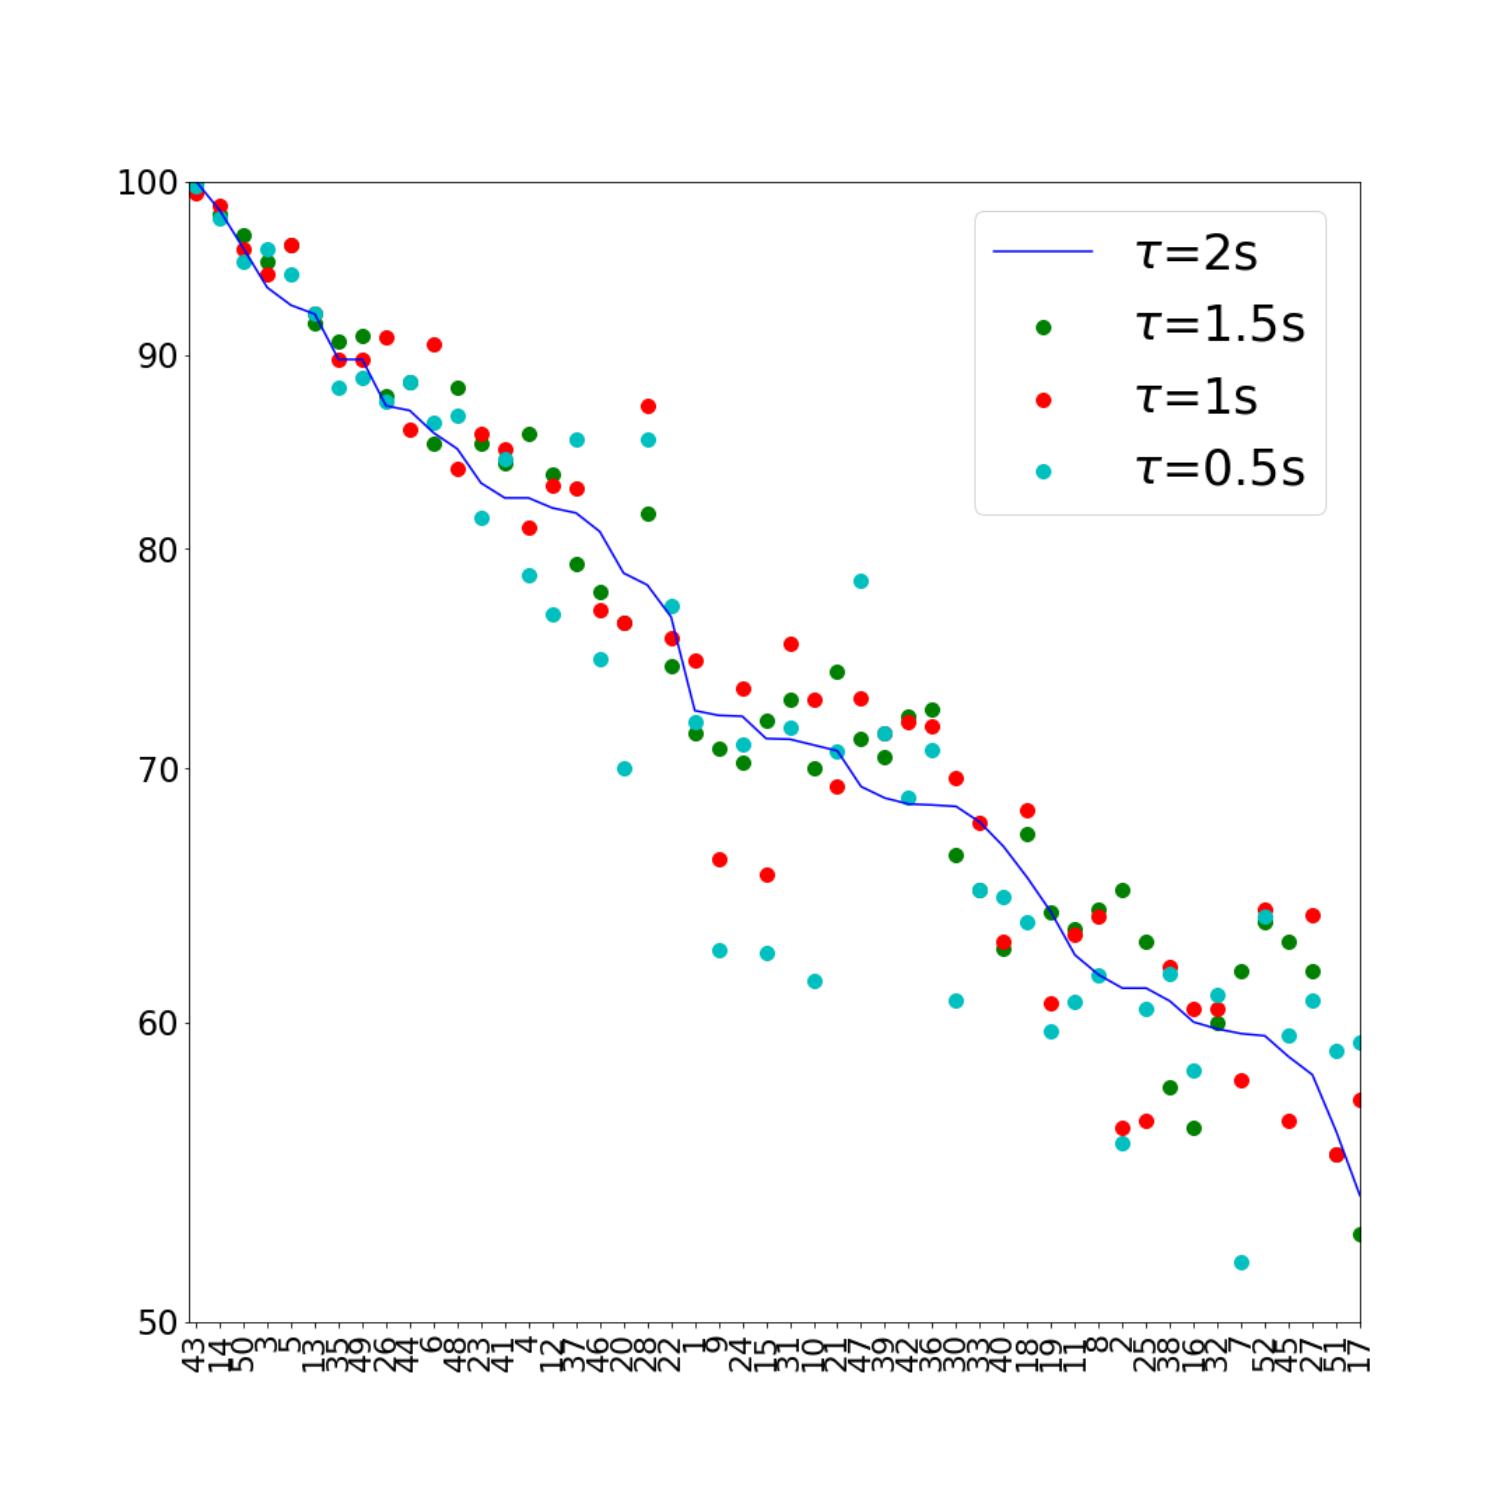
\includegraphics[trim=85 100 80 80, clip]{Figures/Objective_1/taus_gauss_giga_MI.png}}}\\
	\rotatebox{90}{\quad \textbf{\tiny DBIII MI-CSP}}
	\rotatebox{90}{ \quad\,\tiny{Accuracy ($\%$)}}
	{\resizebox{\kerrwidth}{!}{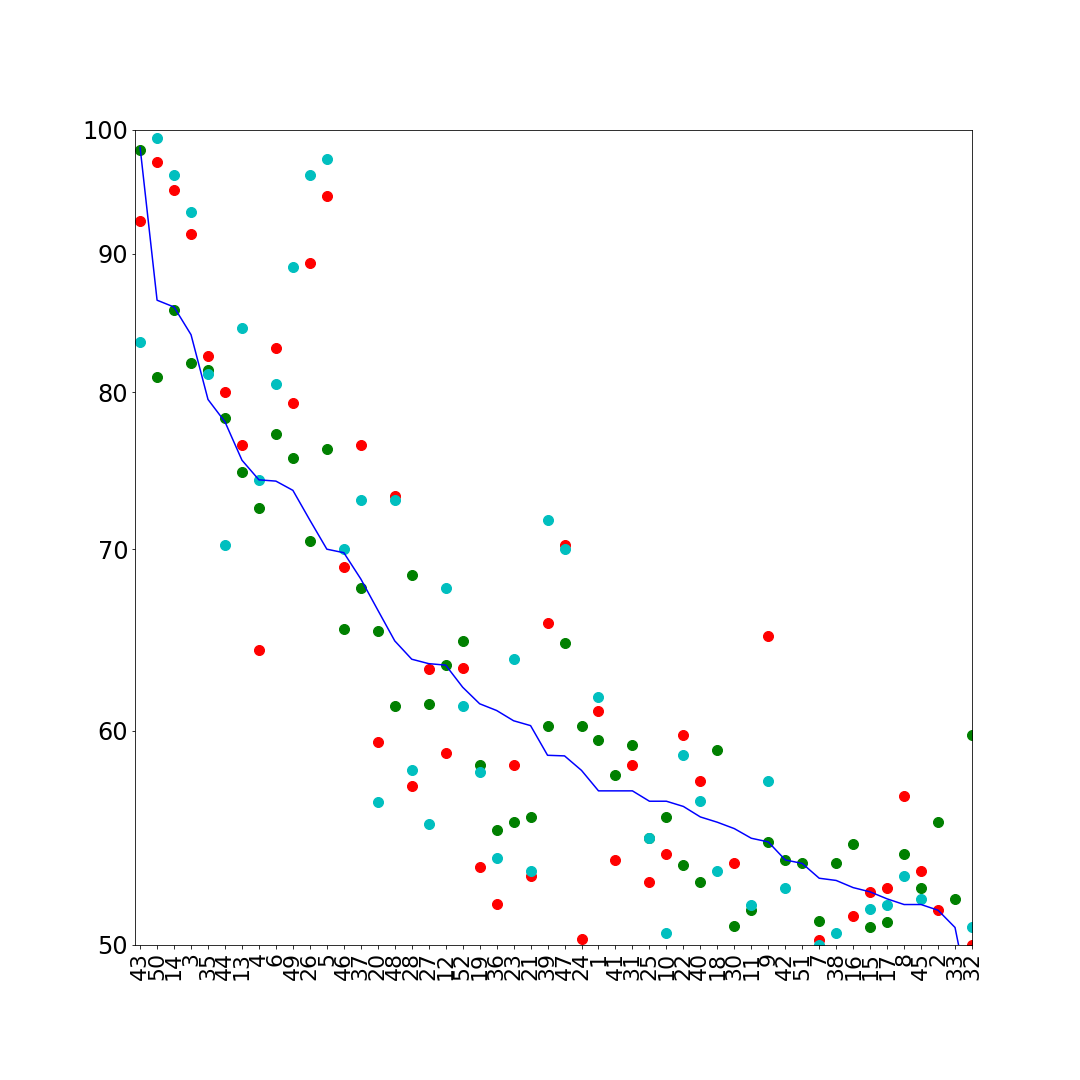
\includegraphics[trim=85 100 80 80, clip]{Figures/Objective_1/taus_csp_plv_giga_MI.png}}}
	{\resizebox{\kerrwidth}{!}{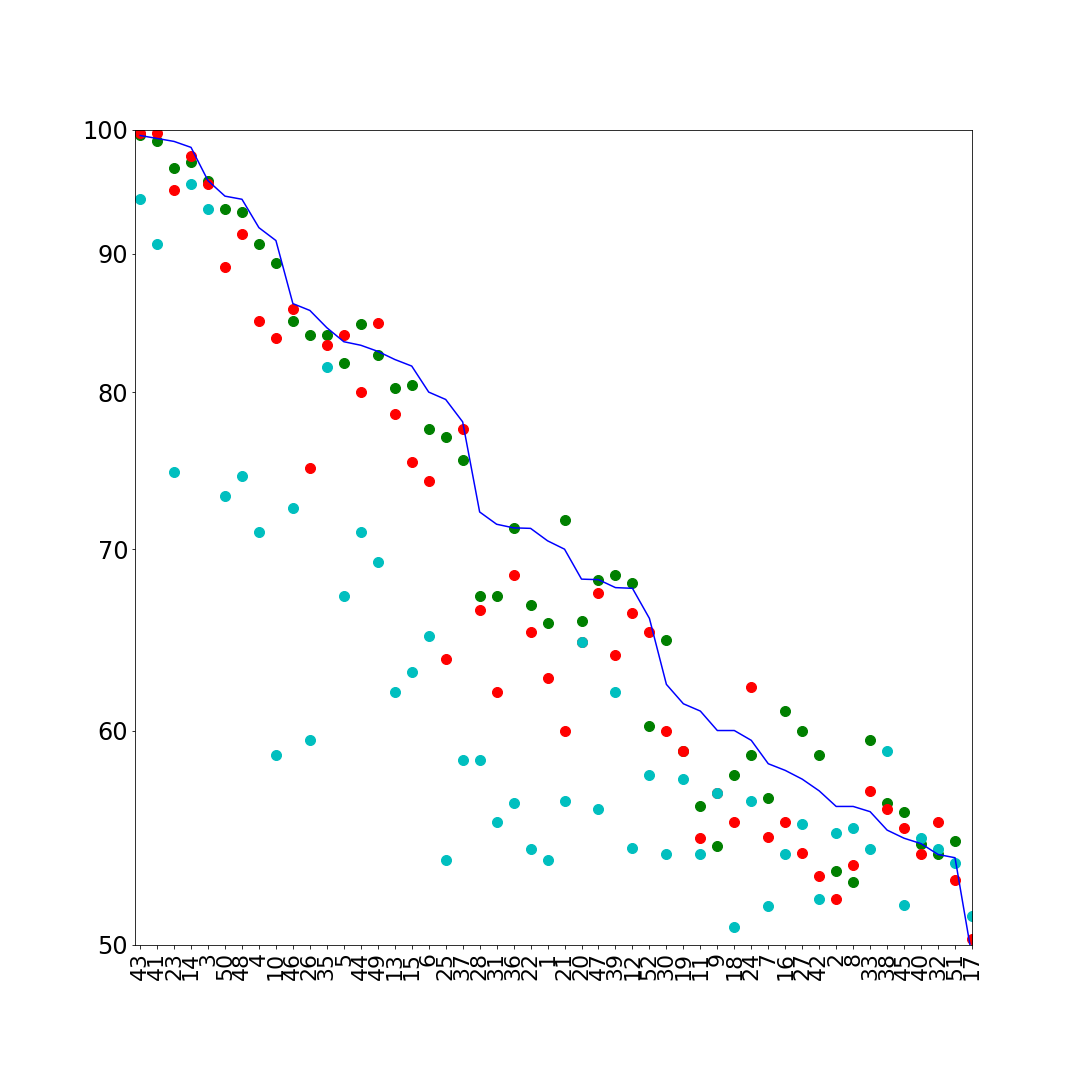
\includegraphics[trim=85 100 80 80, clip]{Figures/Objective_1/taus_csp_pearson_giga_MI.png}}}
	{\resizebox{\kerrwidth}{!}{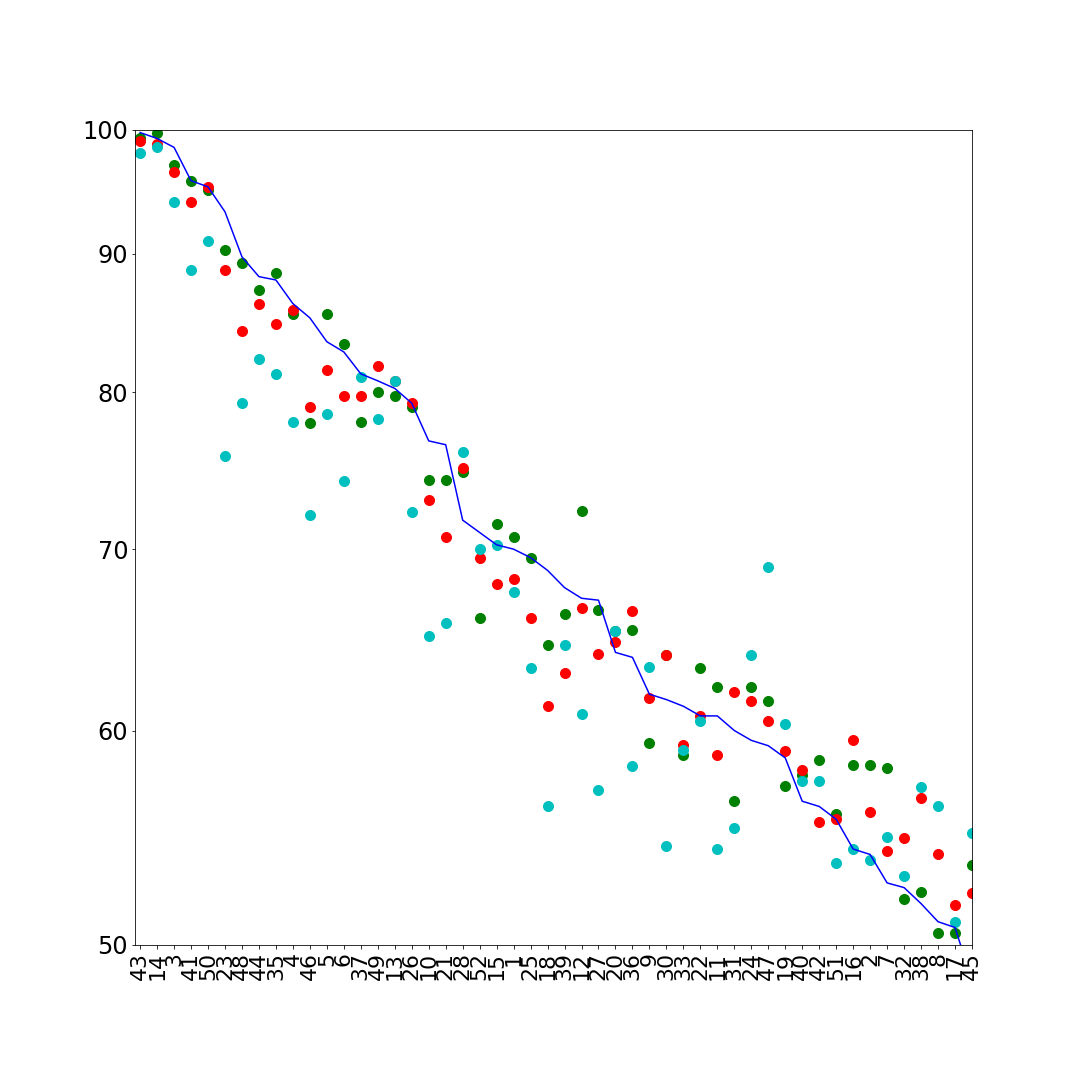
\includegraphics[trim=85 100 80 80, clip]{Figures/Objective_1/taus_csp_gauss_giga_MI.png}}}\\
	\hbox{\hspace{1.9cm} \tiny{Subject id}\hspace{2.8cm} \tiny{Subject id}\hspace{2.9cm} \tiny{Subject id}}
	\caption{{Subject accuracy at each window length $\tau$ performed by the evaluated FC measures: PLV,~CCF, and KCS-FC. Subjects are displayed on the horizontal axis in decreasing order of each FC accuracy at $\tau=2$\,{s}. Notation CSP stands for the accuracy estimated after the spatial CSP filtering.} }\label{Fig:FCx}
\end{figure}

\def \kerrwidth {0.93\linewidth} 
\begin{figure}[h!]
\centering
	\rotatebox{90}{\qquad \quad\, \textbf{DBI-MI}}
	\rotatebox{90}{\qquad \quad\, \footnotesize{Accuracy ($\%$)}}
	{\resizebox{\kerrwidth}{!}{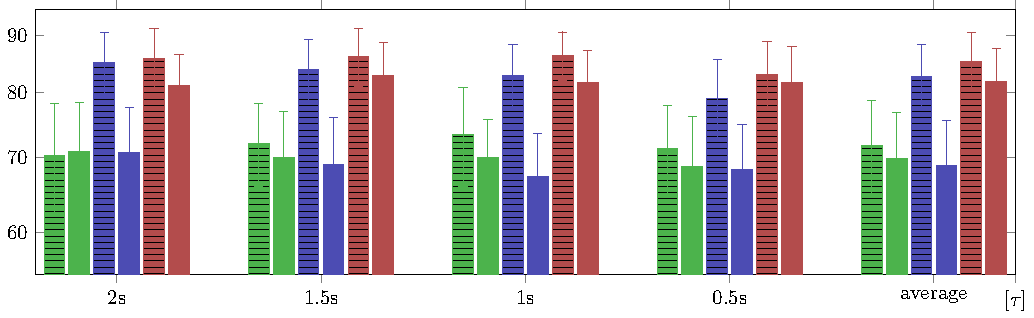
\includegraphics{Figures/Objective_1/acc_regularizacionDBII}}}\\
	\rotatebox{90}{\qquad \quad\, \textbf{DBII-ME}}
	\rotatebox{90}{\qquad \quad\,\footnotesize{Accuracy ($\%$)}}
	{\resizebox{\kerrwidth}{!}{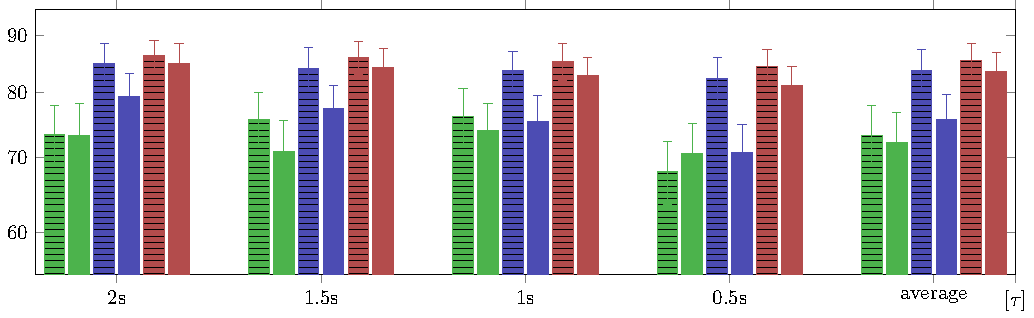
\includegraphics{Figures/Objective_1/acc_regularizacionHG_ME}}}\\
	\rotatebox{90}{\qquad \quad\, \textbf{DBIII-MI}}
	\rotatebox{90}{\qquad \quad\, \footnotesize{Accuracy ($\%$)}}
	{\resizebox{\kerrwidth}{!}{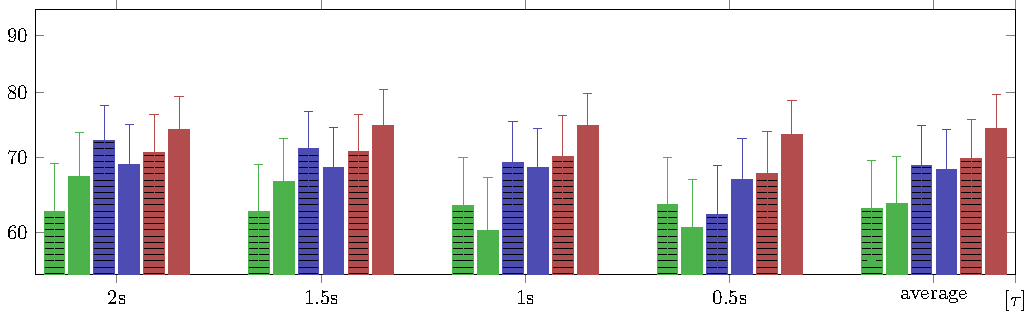
\includegraphics{Figures/Objective_1/acc_regularizacion}}} \\
	\hbox{\hspace{6cm} \textbf{Window length}}
	\caption{Accuracy performed at each $\tau$ by the evaluated measures of FC: PLV(\legend{green!40!gray}),~CCF(\legend{blue!40!gray}), and KCS-FC (\legend{red!40!gray}). {The full-filled colored bars stand for concatenate representation, while the bars with horizontal lines present the results after CSP filtering.}}\label{Fig:AccTau}
\end{figure}

At first sight, besides being distinctive from the CCF and GCF, the variability of accuracy estimates that are achieved by PLV (green line) becomes visible across the subject set of DBII ME: the shorter the window length, the more variable the subject estimates. Rather, the CCF and KCS-FC measures produce accuracy values following a similar order of subjects, for which the enhancing effect of CSP-based filtering can be observed. In the case of DBIII MI, the variability in classifier performance that is provided by the FC metrics grows noticeably, regardless of applying the CSP filtering. Thus, the order of subjects provided by each FC measure is particular and dissimilar to each other. Nevertheless, when compared with the baseline CCF-based accuracy (blue line), the proposed GCF measure without CSP allows for enhancing almost every single subject's discrimination ability, regardless of the window length applied. Moreover, the kernel-based FC measure ensures that several subjects exceed the BCI-inefficiency level, as previously assessed using CCF. It is noteworthy that using the CSP algorithm appreciably reduces the KCS-FC effectiveness for dealing with the subject variability of DBIII MI. 

\def \kerrwidth {0.44\linewidth} 
\begin{figure}[h!]
	\hbox{\hspace{3.3cm} \textbf{DBII-ME}\hspace{4.7cm} \textbf{DBIII-MI}}
	\rotatebox{90}{\qquad \,\footnotesize{Window size}}
	\rotatebox{90}{\qquad \, \footnotesize{$\tau= 2.0$\,{s}}}
	\rotatebox{90}{\qquad \,\tiny{Accuracy ($\%$)}}
	{\resizebox{\kerrwidth }{!}{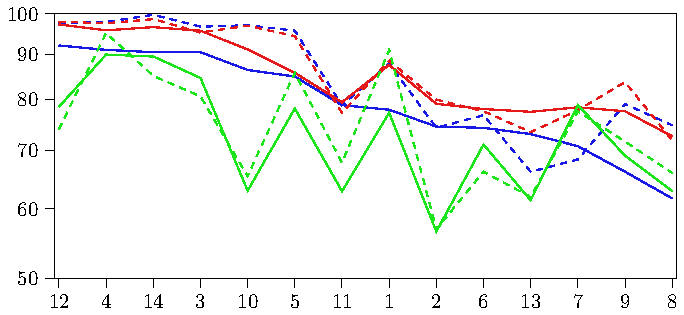
\includegraphics{Figures/Objective_1/ptau2-hg-Me}}}
	{\resizebox{\kerrwidth }{!}{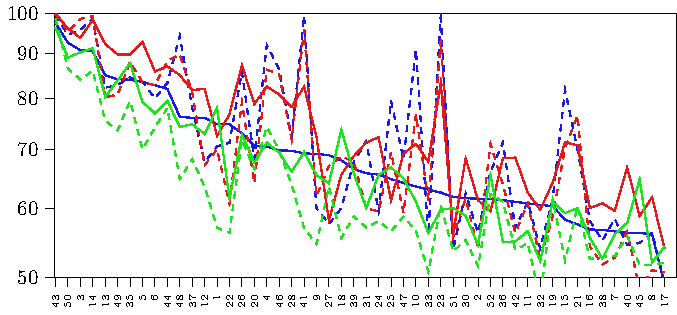
\includegraphics{Figures/Objective_1/ptau2-giga-Mi}}} \\
	\rotatebox{90}{\qquad \,\footnotesize{Window size}}	
	\rotatebox{90}{\qquad \, \footnotesize{$\tau= 1.5$\,{s}}}
	\rotatebox{90}{\qquad \,\tiny{Accuracy ($\%$)}}
	{\resizebox{\kerrwidth }{!}{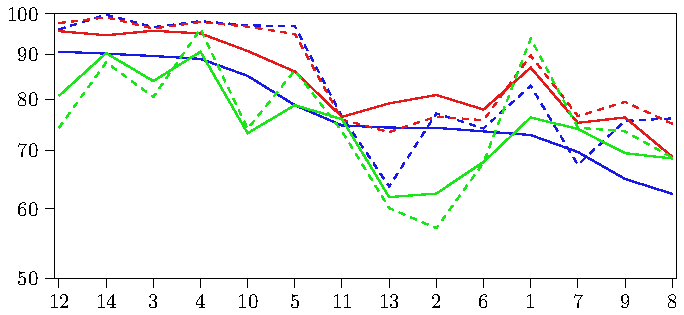
\includegraphics{Figures/Objective_1/ptau1_5-hg-Me}}}
	{\resizebox{\kerrwidth }{!}{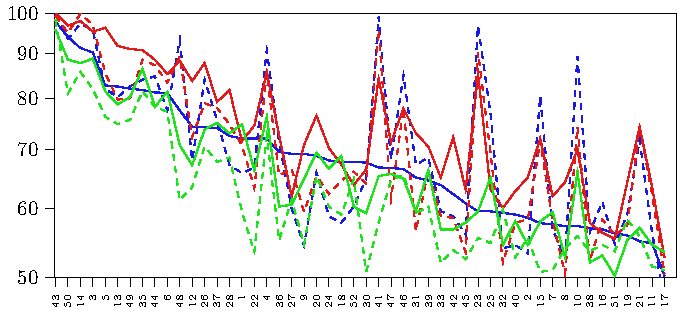
\includegraphics{Figures/Objective_1/ptau1_5-giga-Mi}}}\\
	\rotatebox{90}{\qquad \,\footnotesize{Window size}}	
	\rotatebox{90}{\qquad \, \footnotesize{$\tau= 1.0$\,{s}}}
	\rotatebox{90}{\qquad \,\tiny{Accuracy ($\%$)}}
	{\resizebox{\kerrwidth }{!}{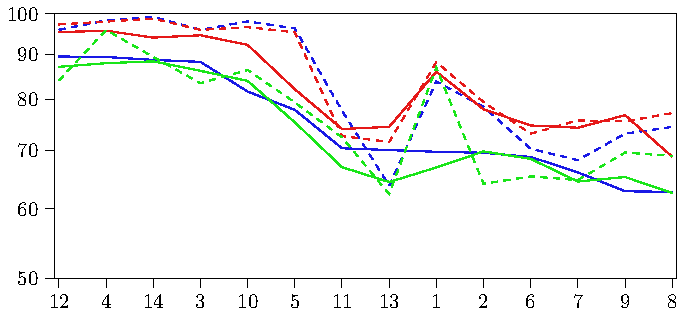
\includegraphics{Figures/Objective_1/ptau1-hg-Me}}}
	{\resizebox{\kerrwidth }{!}{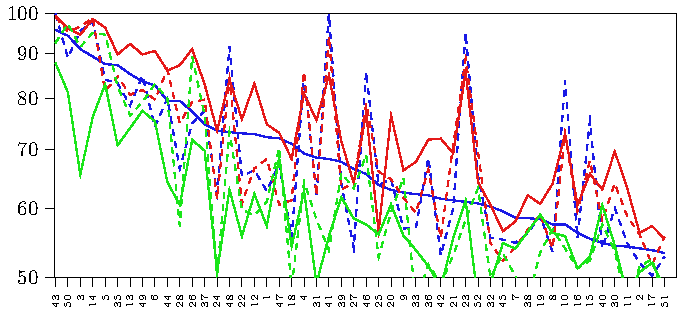
\includegraphics{Figures/Objective_1/ptau1-giga-Mi}}}\\
	\rotatebox{90}{\qquad \,\footnotesize{Window size}}	
	\rotatebox{90}{\qquad \, \footnotesize{$\tau= 0.5$\,{s}}}
	\rotatebox{90}{\qquad \,\tiny{Accuracy ($\%$)}}
	{\resizebox{\kerrwidth }{!}{\includegraphics{Figures/Objective_1/ptau0_5-hg-Me}}}
	{\resizebox{\kerrwidth }{!}{\includegraphics{Figures/Objective_1/ptau0_5-giga-Mi}}} \\
	\hbox{\hspace{3.3cm} \footnotesize{Subject id}\hspace{5.1cm} \footnotesize{Subject id}}
	\caption{Individual classifier performance at different window lengths using FC: PLV (${\lineplot{color5}}$), CCF (${\lineplot{color1}}$), and KCS-FC (${\lineplot{color3}}$). The accuracy assessments performed without CSP are outlined with a continuous line, after CSP filtering---with a dashed line. The subjects are displayed on the horizontal axis in decreasing order of their CCF-based accuracy.}
	\label{Fig:IndividualAcc}
\end{figure}

\subsection{Interpretation of Subject Clusters Using Functional Connectivity Patterns}

The main goal can be framed as the grouping of subjects having similar spatial networks involved in the motor-related tasks under consideration, aiming to properly interpret the evaluated functional connectivity measures. {To this end, we cluster the extracted FC sets into partitions, each one with resembling subjects in terms of FC dynamics, being coded in the relevance vector $\ve{v}$ of Equation~\eqref{eq:SRC}, and the motor-related accuracy. However, because of the poor clustering performance in high dimensional spaces, we accomplish a previous dimensional reduction stage on the normalized subject's relevance vector set (fixing a 2D low-dimensionality) through t-Distributed Stochastic Neighbor Embedding (t-SNE), which preserves the spatial relationships in the higher space (nearest-neighbors)~\cite{linderman2019clustering}. Subsequently, we concatenate the t-SNE low-dimensional representation with the corresponding individual accuracy to perform a {k}-means-based clustering. At each window length, the latter approach is carried out, as proposed in~\cite{Kim2019}.}

One concern is how a subject may switch between the assigned clusters when accounting for the influence of extracted FC measures at each window length. To clarify this aspect, Figure \ref{Fig:clust} displays the clustering results achieved by each functional connectivity measure using a matrix that illustrates the cells colored according to the individual group assessed, ranking the assessed groups in decreasing order of accuracy averaged over the corresponding subset. The three groups are colored, as follows: Group I, giving the best accuracy I (in yellow), Group II with regular accuracy (purple), and Group III, performing the worst accuracy (Turquoise).

\def \kerrwidthME {.32\linewidth}
\def \kerrwidthMI {.55\linewidth}
\begin{figure}[h!]	
\centering
	\hbox{\hspace{2.1cm} \textbf{DBII~ME}\hspace{5cm} \textbf{DBIII~MI}}
	\rotatebox{90}{\qquad {PLV}} 
	\rotatebox{90}{\quad \,\footnotesize{Window size}}	
	{\resizebox{\kerrwidthME}{!}{\includegraphics{Figures/Objective_1/plv_hg}}}
	{\resizebox{\kerrwidthMI}{!}{\includegraphics{Figures/Objective_1/plv_giga}}}\\
	\rotatebox{90}{\qquad {CCF}} 
	\rotatebox{90}{\quad \,\footnotesize{Window size}}		
	{\resizebox{\kerrwidthME}{!}{\includegraphics{Figures/Objective_1/pearson_hg}}}
	{\resizebox{\kerrwidthMI}{!}{\includegraphics{Figures/Objective_1/pearson_giga}}}\\
	\rotatebox{90}{\qquad {KCS-FC}} 
	\rotatebox{90}{\quad \,\footnotesize{Window size}}		
	{\resizebox{\kerrwidthME}{!}{\includegraphics{Figures/Objective_1/gauss_hg}}}
	{\resizebox{\kerrwidthMI}{!}{\includegraphics{Figures/Objective_1/gauss_giga}}}\\
	\hbox{\hspace{2.1cm} \footnotesize{Subject id}\hspace{5cm} \footnotesize{Subject id}}
	\caption{Clustering variability of individuals that belong to Group I (cells in yellow), {Group II (Turquoise), and Group III (purple)}, depending on the extracting window length $\tau$.} \label{Fig:clust}	
\end{figure} 

{As seen for DBII ME, the intragroup similarity remains comparable in groups I and III over the values of $\tau$, while Group II has noticeable volatile behavior}. This result may be explained because of the low number of database subjects (only 14), making any exchange seriously affect the intergroup distribution. In DBIII MI, the high subject variability that is reflected by the functional connectivity extracted yields high changeability between groups, at least for the PLV and CCF measures. Rather, the proposed KCS-FC measure is less affected, as seen at window values of $2$ and $1.5$\,{s}. Further, groups II and III become scrambled, meaning that the subject variability extracted at the shorter window lengths remains hard to overcome. 

The last aspect of the study is the interpretability of motor-related tasks as reliable sources of neural responses in the assessed clusters of dynamic behavior (the groups are denoted as I, II, and III).

{\Cref{Fig:Topograms} presents the topographic channel plots (topoplots) that contain the relevant activated scalp areas that are inferred from the extracted FC measures, principally contributing to the discriminability between labeled motor-related tasks. We also include the most relevant pairwise functional connectivity links between electrodes that are estimated to fulfill the $99$ percentile of the normalized relevance weights values (between 0 to 1) computed from Equation~\eqref{eq:SRC}. The background stands for the accumulated relevance that is mapped to the channel positions.} In DBII ME, only the SMR area is depicted according to the electrode set configuration above-described. 

PLV performs in DBII ME the first three plots in the top row. The topoplots reflect high evoked response amplitudes that are densely spread over the SMR area, which means that the PLV variability hampers the sparse feature selection framework to obtain a reduced set of extracted FC features. Still, a few links surpass the $99$ percentile, which enables some information regarding the relevant electrodes. Contrary to this, the three topoplots that are delivered by CCF (middle row) and KCS-FC (bottom row) show low amplitudes of neural activity in Group I, slightly increased activity of Group II, and increased amplitudes of the worst-performing group of individuals (III). However, the latter FC measure clearly shows two foci that are symmetrically located over each hemisphere, as expected in motor-related tasks, at least for GI and, to a less extent, for GII. Besides, the amount of relevant links estimated is low. Consequently, the sparse-based $\ell_2$-norm framework enables the effective dimensionality reduction of the extracted KCS-FC features. Moreover, the accuracy using KCS-FC assessed by every group of individuals outperforms the other compared functional connectivity metrics: PLV and CCF. 

\nointerlineskip
\def \kerrwidth {0.15\linewidth}
\def \kerrwidthc {0.022\linewidth}
\def \kerrg {0.12\linewidth}
\def \kerrgg {0.05\linewidth}
\def \kerrggg {0.04\linewidth}
%\begingroup
\tabcolsep = 2.0pt
\def\arraystretch{1.0}
\begin{figure}[h!]
%\widefigure
\scalebox{0.95}[0.95]{\begin{tabular}{cccccccc}
\centering
& & \textbf{DBII~ME}& & & \textbf{DBIII~MI}&\\
\cmidrule{2-7}
& {I} & {II}&{III}&{I} & {II}&{III}&
\multirow{6}{*}{{\includegraphics[trim=660 0 0 0, clip,scale=0.35]{Figures/Objective_1/Cxsbj1hg-gaussacc95.28.eps}}}\\
\cmidrule{2-7}
& \textbf{$84.13\%$}& \textbf{$74.91\%$} & \textbf{$64.21\%$} & \textbf{$72.2\%$} & \textbf{$68.76\%$} & \textbf{$55.94\%$}&\\
{\rotatebox{90}{\hspace{7mm} {PLV}}}&{\resizebox{\kerrwidth}{!}{\includegraphics[trim=100 120 90 90, clip]{Figures/Objective_1/Cxsbj1hg-plvacc84.13.eps}}}&
	{\resizebox{\kerrwidth}{!}{\includegraphics[trim=100 120 90 90, clip]{Figures/Objective_1/Cxsbj2hg-plvacc74.91.eps}}}&
	{\resizebox{\kerrwidth}{!}{\includegraphics[trim=100 120 90 90, clip]{Figures/Objective_1/Cxsbj3hg-plvacc64.21.eps}}}&
	{\resizebox{\kerrwidth}{!}{\includegraphics[trim=100 120 90 90, clip]{Figures/Objective_1/Cxsbj1plvacc72.2.eps}}}&
	{\resizebox{\kerrwidth}{!}{\includegraphics[trim=100 120 90 90, clip]{Figures/Objective_1/Cxsbj2plvacc68.76.eps}}}&
	{\resizebox{\kerrwidth}{!}{\includegraphics[trim=100 120 90 90, clip]{Figures/Objective_1/Cxsbj3plvacc55.94.eps}}}&\\
	& \textbf{$90.06\%$} & \textbf{$79.35\%$} & \textbf{$70.59\%$} &  \textbf{$76.67\%$} & \textbf{$64.62\%$} & \textbf{$60.69\%$}&\\
	\rotatebox{90}{\hspace{7mm} {CCF}}&
	{\resizebox{\kerrwidth}{!}{\includegraphics[trim=100 120 90 90, clip]{Figures/Objective_1/Cxsbj1hg-pearsonacc90.06.eps}}}&
	{\resizebox{\kerrwidth}{!}{\includegraphics[trim=100 120 90 90, clip]{Figures/Objective_1/Cxsbj2hg-pearsonacc79.35.eps}}}&
	{\resizebox{\kerrwidth}{!}{\includegraphics[trim=100 120 90 90, clip]{Figures/Objective_1/Cxsbj3hg-pearsonacc70.59.eps}}}&
	{\resizebox{\kerrwidth}{!}{\includegraphics[trim=100 120 90 90, clip]{Figures/Objective_1/Cxsbj1pearsonacc76.67.eps}}}&
	{\resizebox{\kerrwidth}{!}{\includegraphics[trim=100 120 90 90, clip]{Figures/Objective_1/Cxsbj2pearsonacc64.62.eps}}}&
	{\resizebox{\kerrwidth}{!}{\includegraphics[trim=100 120 90 90, clip]{Figures/Objective_1/Cxsbj3pearsonacc60.69.eps}}}&\\
	& \textbf{$\mathbf{95.28}\%$}& \textbf{$\mathbf{81.16}\%$}& \textbf{$\mathbf{76.09}\%$}& \textbf{$\mathbf{86.85}\%$}& \textbf{$\mathbf{68.93}\%$}& \textbf{$\mathbf{64.4}5\%$}&\\
	\rotatebox{90}{\hspace{7mm} {KCS-FC}}&
	{\resizebox{\kerrwidth}{!}{\includegraphics[trim=100 120 90 90, clip]{Figures/Objective_1/Cxsbj1hg-gaussacc95.28.eps}}}&
	{\resizebox{\kerrwidth}{!}{\includegraphics[trim=100 120 90 90, clip]{Figures/Objective_1/Cxsbj2hg-gaussacc81.16.eps}}}&
	{\resizebox{\kerrwidth}{!}{\includegraphics[trim=100 120 90 90, clip]{Figures/Objective_1/Cxsbj3hg-gaussacc76.09.eps}}}&
	{\resizebox{\kerrwidth}{!}{\includegraphics[trim=100 120 90 90, clip]{Figures/Objective_1/Cxsbj1gaussacc86.85.eps}}}&
	{\resizebox{\kerrwidth}{!}{\includegraphics[trim=100 120 90 90, clip]{Figures/Objective_1/Cxsbj2gaussacc68.93.eps}}}&
	{\resizebox{\kerrwidth}{!}{\includegraphics[trim=100 120 90 90, clip]{Figures/Objective_1/Cxsbj3gaussacc64.45.eps}}}&\\
	&\multicolumn{6}{c}{\resizebox{0.85\linewidth}{!}{\includegraphics[trim=0 0 50 600, clip]{Figures/Objective_1/Cxsbj1hg-gaussacc95.28.eps}}}&
\end{tabular}}
\vspace{-42pt}
\caption{Spatial
 relevance mapped to topoplots estimated for each group of individuals from the FC measures (regarding the relevance weights $\ve{v}$ and the classification accuracy). The normalized relevance weights values (between 0 to 1) are computed from Equation~\eqref{eq:SRC}. The background stands for the accumulated spatial relevance mapped to the EEG channel positions. The colored links represent the normalized FC relevance weights that hold a value higher than the $99$ percentile of vector $\ve{v}$. Above each plot, the average accuracy is shown over the corresponding group.}\label{Fig:Topograms}
\end{figure}

In DBIII~ME, the full electrode montage is employed and, thus, the estimated neural responses are all spread over the scalp, as seen in the three last topoplots of every row. Likewise, the number of relevant links increases. Nonetheless, the compared FC measures' performance has some similarities with DBII MI: PLV presents high background activity, CCF has amplitudes with fewer amplitudes, and GCF achieves a very focalized activity over the SMR hemispheres, which play a critical role in MI tasks. Once again, the proposed KCS-FC measure outperforms the values of accuracy attained by other compared FC metrics. However, G III produces highly increased response amplitudes abnormally confined over the frontal zone (outside the SMR zone) and numerous links going to different electrodes. This issue may be explained because of acquisition artifacts, which may introduce noise and distortions, severely damaging the EEG data quality.

\subsection{Selecting the Sliding Time Window} 

The window length selected for extracting the EEG dynamics over time is a pivotal parameter. From the results obtained, both contrasted single-trial FC measures (Cross-Correlation Coefficient and Phase Lag Value) show several fluctuations over the evaluated values of $\tau$ that diminish the performed accuracy, becoming worse in databases with increased subject variability, as is the case of DBIII MI. On the other hand, the proposed Gaussian Functional Connectivity measure enables accuracy estimates that are less affected by the sliding time window and, thus, KCS-FC allows for extracting the subject's dynamics more accurately within wider ranges of $\tau$. 

\subsection{Prior Spatial Filtering Versus to Feed the Concatenation of FC Feature Sets} 

\begin{table}[h!]
	\caption{Classifier accuracy comparison of approaches using functional connectivity features recently reported against the Gaussian FC performance in discriminating MI tasks. Notation TSGSP is temporally constrained sparse group spatial pattern, STR is space-time recurrence, and OPTICAL is Optimized CSP with long short term memory (LSTM). The best value performed for each database is marked in bold.} \label{Tab:Acc}
	\setlength{\tabcolsep}{4.9mm}

\resizebox{\columnwidth}{!}{
\begin{tabular}{cccccc}
	\toprule
		\textbf{Data}& \textbf{Time Window} & \textbf{Filter Band} & \textbf{Interpretation} & \textbf{Feature Extraction}  & \textbf{Accuracy} (\%)\\
		\midrule
		{\multirow{4}{*}{\rotatebox[origin=c]{90}{{DBI-MI}%MDPI: please confirm the text direction. We confirm.
}}} &
		\checkmark&\checkmark&\checkmark&TSGSP~\cite{Zhang2018}&\textbf{82.50} $\pm$ \textbf{12.2}\\
		&-&-&\checkmark&STR connectivity~\cite{rodrigue2019}&69.56$\pm$15.02\\
		& \checkmark & - & \checkmark & Renyi's $\alpha$-entropy~\cite{de2019data} & 72.40 $\pm$ 6.50\\					
		&\checkmark&\checkmark&\checkmark&{Proposed KCS-FC}& {81.92} $\pm$ {9.44}\\
		\midrule	
		{\multirow{4}{*}{\rotatebox[origin=c]{90}{DBIII-MI}}} &		
		- &\checkmark&\checkmark & CSP~\cite{cho2017eeg}&67.60 $\pm$ 13.17\\
		&\checkmark&\checkmark&-&OPTICAL~\cite{kumar2019brain}&68.19 $\pm$ 9.36\\
		&-&-&\checkmark&STR connectivity~\cite{rodrigue2019}&62.00 $\pm$ 13.00\\	
		&\checkmark&\checkmark&\checkmark&{Proposed KCS-FC}&\textbf{74.12} $\pm$ \textbf{12.13} \\\bottomrule
	\end{tabular}
 }
\end{table}

Because of the poor signal-to-noise ratio of scalp EEG measurements, the baseline CSP-based spatial filtering is very frequently accomplished. Meanwhile, the evaluating results indicate that the CSP effectiveness degrades noticeably as the inter/intrasubject variability increases. Thus, a big partition of subjects in DBIII MI turns out to be below the BCI-inefficiency level. These findings are according to the reported CSP variability from trial-to-trial~\cite{Gaur2021}, and the subject-dependent choice of its extraction window~\cite{Velasquez-Martinez2020}. 

One more restriction is that CSP is more oriented to power-based features~\cite{kumar2018eeg}, so that its validity of the combination with PLV is questionable, as the achieved results definitely indicate. The combination of CSP with CCF and KCS-FC allows for enhancing the performed accuracy, but in DBI~MI and DBII~ME with a relatively moderate number of subjects. The testing of DBIII~MI with the largest considered intra/inter-subject variability tends to nullify CSP filtering before CCF feature extraction. Moreover, the proposed KCS-FC measures' performance improves if avoiding using the spatial filtering algorithm, which means that FC feature sets' straightforward concatenation is enough to feed the sparse-based $\ell_2$-norm feature selection framework. Table \ref{Tab:Acc} displays the evaluated MI data's accuracy (i.e.,~DBI MI, and DBIII MI) using functional connectivity measures that have been reported recently, noting that the proposed KCS-FC approach provides very competitive classifier performance values.



\section{Summary}

We have introduced a novel method for single-trial kernel cross-spectral functional connectivity, known as KCS-FC, which addresses prevalent challenges inherent to EEG-based MI-BCI systems, identified in \cref{sec:singlefc}. These include issues related to non-stationarity, non-linearity, inter-subject variability, and spurious connectivities. To achieve this, we applied an extension of Bochner's theorem to approximate the cross-spectral distribution as a weighted sum of Gaussian-kernel-based pairwise relationships between channels, considering various time windows and frequency sub-bands. This weighted sum is managed by a linear regression model combined with an elastic net regularization that aligneds the value with the MI label and differentiates spurious connectivities. In testing our method, we compared it with two prevalent single-trial FC estimators and respective CSP versions using two publicly available MI datasets. The results reveal that our KCS-FC strategy shows competitive accuracy in performance while maintaining interpretable FC matrices.

However, our approach heavily relies on handcrafted feature extraction processes, including time windowing and sub-band selection. This reliance on handcrafted features, as discussed in \cref{sec:problem2}, does not significantly assist in artifact removal and only marginally increases accuracy for lower-performing individuals. Future research, as suggested in \cref{sec:sota2}, should focus on adopting end-to-end DL models that can autonomously extract EEG representations. This would potentially be more effective in removing artifacts and could potentially enhance the performance of low-performing individuals.

%\chapter{\Objectivetwoname}
\chapter[Kernel Cross-Spectral Functional Connectivity Network]{KCS-FCnet: Kernel Cross-Spectral Functional Connectivity Network for Automatic EEG Representation in MI-BCI}\label{chapter_2}


Here we propose an end-to-end technique for classifying MI using EEG signals, termed Kernel Cross-Spectral Functional Connectivity Network (KCS-FCnet), as depicted in \cref{fig:contribution2}. Our approach overcomes current DL limitations by introducing a cross-spectral Gaussian functional connectivity data-driven estimator to classify MI tasks from raw data. KCS-FCnet utilizes 1D convolutional layers to extract temporal-frequency features from input channels and a cross-spectral distribution estimation that codes relevant temporal and spectral MI patterns. It also includes a functional connectivity feature map, which improves the interpretability of the model by extracting meaningful pairwise channel relationships. Our approach is evaluated on a publicly available dataset and achieves state-of-the-art results for EEG-based MI classification. Furthermore, it demonstrated robustness to different experimental settings and individual differences. Lastly, our results suggest that the KCS-FCnet architecture is a highly effective method for EEG-based MI classification and can potentially be applied in real-world BCI.

\begin{figure}[h!]
    \centering
    \includegraphics[scale=0.6]{Figures/outline_and_contributions/contribution2.pdf}
    \caption{Schematic diagram illustrating the proposed Kernel Cross-Spectral FC Network (KCS-FCnet), including the use of DL strategies and a CNN layer for artifact removal and spectral and temporal feature extraction. The diagram further outlines the process of spatial extraction via a custom layer incorporating the kernel cross-spectral function}\label{fig:contribution2}
\end{figure}

\section{Kernel Cross-Spectral Functional Connectivity Network}\label{sec:gcnet}
	
	The input-output EEG dataset, $\{\mat{X}_r \in \Real^{N_c \times N_t}, \ve{y}_r \in\{0,1\}^{N_y}\}^R_{r=1}$, comprises $R$ trials, $N_t$ time instants, $N_c$ channels, and $N_y$ classes. To enhance the most informative EEG spatial-temporal-spectral patterns from $\mat{X}_r$ and reduce noise for improved MI class prediction, we propose to estimate the cross-spectral distribution among channels using a function composition. This approach gathers 1-D convolutional-based feature layers for extracting time-frequency patterns within each EEG channel and a Gaussian kernel-based pairwise similarity, as follows:
	\changes{
	\begin{equation}\label{eq:CSf}
		\hat{\mat{P}}_{r}(\ve{w}_f)  = \tilde{K}(\cdot;\sigma) \circ \varphi(\mat{X}_r; \ve{w}_f), 
	\end{equation}
	where $\hat{\mat{P}}_{r}~(\ve{w}_f)~\in~[0,1]^{N_c\times N_c \times N_f}$, $N_f$ is the number of convolutional filters, notation $\circ$ stands for function composition, $\varphi(\cdot; \mat{w}_f)$ is a 1-D convolutional layer that can be used to automatically extract frequency patterns ruled by the weight vector $\ve{w}_f\in \Real^{\Delta_t}$, with $\Delta_t<N_t.$ Of note, in Equation \eqref{eq:CSf} function $\tilde{K}(\cdot;\sigma)$ is the convolutional filter concatenation of all pair-wise values $\kappa_{x}(\ve{x}^{c}_{rf},\ve{x^{c'}_{rf}}; \sigma)$ and is obtained as:
    \begin{equation}
        \tilde{K}(\mat{\tilde{X}}_r;\sigma) = \left[ \mat{K}_{r1} , \mat{K}_{r2}, \cdots,\mat{K}_{rf},\cdots, \mat{K}_{rN_f} \right],
    \end{equation}
    where $\mat{K}_{rf} \in \Real^{N_c \times N_c}$ is the kernel matrix for a trial $r$ at a convolutional filter $f$ and it is calculated as follows:
    \begin{equation}
        \mat{K}_{rf} = \begin{bmatrix}
            \kappa_{x}(\ve{x}^{1}_{rf}, \ve{x}^{1}_{rf}; \sigma) & \kappa_{x}(\ve{x}^{1}_{rf}, \ve{x}^{2}_{rf}; \sigma) & \cdots & \kappa_{x}(\ve{x}^{1}_{rf}, \ve{x}^{N_c}_{rf}; \sigma) \\
            \kappa_{x}(\ve{x}^{2}_{rf}, \ve{x}^{1}_{rf}; \sigma) & \kappa_{x}(\ve{x}^{2}_{rf}, \ve{x}^{2}_{rf}; \sigma) & \cdots & \kappa_{x}(\ve{x}^{2}_{rf}, \ve{x}^{N_c}_{rf}; \sigma) \\
            \vdots & \vdots & \ddots & \vdots \\
            \kappa_{x}(\ve{x}^{N_c}_{rf}, \ve{x}^{1}_{rf}; \sigma) & \kappa_{x}(\ve{x}^{N_c}_{rf}, \ve{x}^{2}_{rf}; \sigma) & \cdots & \kappa_{x}(\ve{x}^{N_c}_{rf}, \ve{x}^{N_c}_{rf}; \sigma).
        \end{bmatrix}
    \end{equation}
    We compute the average functional connectivity measure $\tilde{\mat{P}}_r \in \Real^{N_c \times N_c}$ over convolutional filters, as follows:
    \begin{equation}
		\tilde{\mat{P}}_r  = \operatorname{AvgPooling}_{f} \left(\hat{\mat{P}}_{r}(\ve{w}_f)\right), \label{eq:lastlayerFC}
	\end{equation}
    where $\ve{w}_f$ is the $f$-th convolutional filter, $N_f$ is the number of convolutional filters. This measure provides a way to analyze how different frequency bands of a single-trial EEG relate to each other across channels. After computing the average functional connectivity measure and taking advantage of the symmetric property of the Gaussian functional connectivity, the vectorized version of $\tilde{\mat{P}}_r$ is calculated as:
    \begin{equation} 
        \overline{\ve{p}}_r = \left[\tilde{p}_r^{12}, \tilde{p}_r^{13}, \cdots, \tilde{p}_r^{cc'}, \cdots, \tilde{p}_r^{(N_c-1) N_c} \right]; \forall c<c',
    \end{equation}
    where $\overline{\ve{p}}_r \in  \Real ^{N_c(N_c-1)/2}$. Next, a the softmax-based output layer is applied over vector $\overline{\ve{p}}_r$ to obtain the MI class probability membership $\hat{\ve{y}}_r \in [0,1]^{N_y}$ as:
    }  
    \changes{
	\begin{equation}\label{eq:output}
		\hat{\ve{y}}_r = {\rm{softmax}}\left(\mat{V}\overline{\ve{p}}_r + \ve{b}\right),
	\end{equation}
	where $\mat{V}\in \Real^{N_c(N_c-1)/2\times N_y}$, $\ve{b} \in \Real^{N_y}$. In addition, a gradient descent-based framework using back-propagation is employed to optimize the parameter set $\Theta=\{\ve{w}_f,\mat{V},\ve{b},\sigma;\forall f\in\{1,2,\dots,N_f\}\},$ as follows~\cite{zhang2021dive}:
    }
    
	\begin{equation}\label{eq:opt}
		\Theta^{*} = \underset{\Theta}{\arg\,\min} \quad \promeddd{r}{\mathcal{L}(\ve{y}_r,\hat{\ve{y}}_r|\Theta); \forall r\in\{1,2,\dots,R\}},
	\end{equation}
	being $\mathcal{L} \{\cdot\}$ a given loss function, i.e., cross-entropy. The optimization problem outlined in Equation~\eqref{eq:opt} enables the training of our Kernel Cross-Spectral Functional Connectivity Network (KCS-FCnet) for the classification of MI tasks. 


\section{Experimental Set-Up} \label{sec:Experiment}

\subsection{KCS-FCnet Implementation Details}

In this study, we evaluate the efficacy of our proposed method for extracting subject-specific functional connectivity matrices from the KCS-FCnet that predicts MI output labels from EEG records. To accomplish this, we have developed a pipeline consisting of the following steps, which were tested on the Giga dataset (as detailed in Section \ref{sec:dataset}): 

\begin{itemize}
    \item[--] {{Raw EEG Preprocessing:} 
    } First, we load subject recordings using a custom databases loader {module} 
    ~(\url{https://github.com/UN-GCPDS/python-gcpds.databases} ({accessed on 27 January 2023}
    )). Next, we downsample each signal from 512 Hz to 128 Hz using the Fourier method provided by the SciPy signal resample function~(\url{https://docs.scipy.org/doc/scipy/reference/generated/scipy.signal.resample.html} ). Then each time series trial was filtered between [4, 40] Hz, using a fifth-order Butterworth bandpass filter. In addition, we clipped the records from 0.5 s to 2.5 s post cue onset, retaining only information from the motor imagery task. Preprocessing step resembles the one provided by authors in~\cite{lawhern2018eegnet}. Note that since we are analyzing only the MI time segment, we assume the signal to be stationary. Our straightforward preprocessing aims to investigate five distinct brain rhythms within the 4 to 40 Hz range, including theta, alpha, and three beta waves. Theta waves (4--8 Hz), located in the hippocampus and various cortical structures, are believed to indicate an ``online state'' and are associated with sensorimotor and mnemonic functions, as stated by authors in \cite{ABHANG201651}. In contrast, sensory stimulation and movements suppress alpha-band activity (8--13 Hz). It is modulated by attention, working memory, and mental tasks, potentially serving as a marker for higher motor control functions. Besides, tested preprocessing also comprises three types of beta waves: Low beta waves (12--15 Hz) or ``beta one'' waves, mainly associated with focused and introverted concentration. Second, mid-range beta waves (15--20 Hz), or ``beta two'' waves, are linked to increased energy, anxiety, and performance. Third, high beta waves (18--40 Hz), or ``beta three'' waves, are associated with significant stress, anxiety, paranoia, high energy, and high arousal.
    
    \item[--] {{KCS-FCnet Training:}} We split trials within each subject data using the standard $5$-{fold} $80${--}$20$ scheme. That means shuffling the data and taking $80\%$ of it to train (training set), holding out the remaining $20\%$ to validate trained models (testing set), and repeating the process five times \cite{schirrmeister2017deep}. For the sake of comparison, we calculate the accuracy, Cohen's kappa, and the area under the ROC curve to compare performance between models~\cite{warrens2015five,geron2022hands}. It is worth noting that we rescale the kernel length according to the new sampling frequency as in \cite{lawhern2018eegnet}. The GridSearchCV class from SKlearn is used to find the best hyperparameter combination of our KCS-FCnet. The number of filters $N_f$ is searched within the set $\{2,3,4\}$.
    
    \item[--] {{Group-Level Analysis:}}  We build a scoring matrix that contains as many rows as subjects in the dataset, 50 for Giga, and six columns, including accuracy, Cohen's kappa, and the area under the ROC curve scores, along with their respective standard deviation. To keep the intuition of the higher, the better, and constrain all columns to be between $[0,1]$ in the score matrix, we replace the standard deviation with its complement and normalize the Cohen's kappa by adding to it the unit and dividing by two. Then, using the score matrix and the k-means clustering algorithm~\cite{geron2022hands}, with $k$ set as three, we trained a model to cluster subjects' results based on the baseline model EEGnet~\cite{lawhern2018eegnet} in one of three groups: best, intermediate, and worst performing subjects. Next, we order each subject based on a projected vector obtained from the first component of the well-known Principal Component Analysis (PCA) algorithm applied to the score matrix. Next, with the trained $k$-means, the subjects analyzed by our KCS-FCnet were clustered using the score matrix. The aim is to compare and check how subjects change between EEGnet and KCS-FCnet-based groups. 
\end{itemize}    
	
A KCS-FCnet sketch can be visualized in \changes{Figure \ref{fig:contribution2}.} The detailed KCS-FCnet architecture is summarized in Table \ref{table:CS-GFCnet}. All experiments were carried out in{ Python 3.8}, with the {Tensorflow 2.4.1 API}, on Google Colaboratory and Kaggle environments. The fine-tuning process for the model's parameters begins by utilizing the training set for optimization. To evaluate the model's performance, the test set is employed solely for reporting scores. The categorical cross-entropy loss function is applied, and no additional callbacks are utilized. The training phase involves passing the entire batch of samples. Additionally, to support further analysis and experimentation, the model weights and performance scores are systematically saved for future reference.

%KCS-FCnet 
	\begin{table}[H]
		\centering
		\caption{Detailed KCS-FCnet architecture for MI classification.}\label{table:CS-GFCnet}
		\begin{tabularx}{\textwidth}{lcc}
			\hline
			\textbf{Layer}     & \textbf{Output Dimension}           & \textbf{Params.}                                                       \\ \midrule
			Input              & $N_c \times N_t \times 1$                 & $\cdot$                                                                  \\
			Conv2D             & $N_c \times (N_t - \Delta_t + 1) \times N_f$     & \begin{tabular}[c]{@{}c@{}}max norm = 2.0, kernel size = (1, $\Delta_t$)\\ Stride size = (1, 1), Bias = False\end{tabular} \\
			BatchNormalization & $N_c \times (N_t - \Delta_t + 1) \times N_f$     & $\cdot$                                                                  \\ \midrule
			\multicolumn{3}{c}{ELU activation}                                                                                               \\ \midrule
			KCS-FCblock           & $N_f \times (N_c \cdot (N_c-1)/2) \times 1$ & $\cdot$                                                                  \\
			AveragePooling2D   & $1 \times (N_c \cdot (N_c-1)/2) \times 1$  & $\cdot$                                                                  \\
			BatchNormalization & $1 \times (N_c \cdot (N_c-1)/2) \times 1$  & $\cdot$                                                                  \\ \midrule
			\multicolumn{3}{c}{ELU activation}                                                                                               \\ \midrule
			Flatten            & $N_c \cdot (N_c-1)/2$                  & $\cdot$                                                                  \\
			Dropout            & $N_c \cdot (N_c-1)/2$                   & Dropout rate = 0.5                                                    \\
			Dense              & $N_y$                                  & max norm = 0.5                                                        \\ \midrule
			\multicolumn{3}{c}{Softmax}                                                                                                      \\ \midrule
		\end{tabularx}
	\end{table}

	\subsection{Functional Connectivity Pruning and Visualization}
	
	To compare functional connectivity between the groups mentioned above, first, we have to check which connections are relevant for class separability. It is worth noting that a high correlation in the functional connectivity matrix does not guarantee a higher class separability. Therefore, we use the two-sample Kolmogorov–Smirnov (2KS) test to overcome this issue and select only relevant connections as in \cite{gu2020random}. The null hypothesis is that both samples are drawn from the same unknown distribution. Thus, we group the trials of each connection for a subject according to the label to build the samples ``right'' and ``left''. Then, every pair is passed through the 2KS test, and connections holding a $p$-value equal to or lower than $0.05$ are kept. Hence, we can state that both samples came from different distributions and the classes are distinguishable. Next, we build a $p$-value matrix containing the information on whether a connection is relevant. To visualize how each $p$-value matrix changes across subjects and groups, we plot each $p$-value matrix on a 2D visualization, where both dimensions are calculated using the well-known $t$-distributed Stochastic Neighbor Embedding ($t$-SNE) algorithm~\cite{van2008visualizing}, from the SKlearn library, over the EEGnet score matrix. It is noteworthy that the perplexity parameter has been specifically set to a value of ten, while all other parameters have been retained at their default settings.
	
	Next, to effectively depict the connections between various regions of the brain, we employ a specialized connectivity visualizer~(\url{https://github.com/UN-GCPDS/python-gcpds.visualizations} ) which utilizes the Circos plot technique to display only the most significant connections, specifically those that fall within the $99$-th percentile. To further enhance the analysis, we have chosen to plot the subject closest to the centroid of each group, thereby allowing for a detailed examination of one individual from each group.
	
	
	\subsection{Method Comparison}
	
	We compare the proposed KCS-FCnet with four end-to-end DL models that have been reported recently for effectively extracting relevantly explainable information from raw EEG. As with our proposal, the contrasted architectures are selected because they benefit from convolutional layers to extract temporal-frequency features for improving MI classification performance. Namely, (i) the EEGnet architecture in~\cite{lawhern2018eegnet} operates depthwise separable convolutions to reduce the number of training parameters, extracting temporal and spatial convolution features from each channel of a previous feature map; (ii) Shallowconvnet in~\cite{schirrmeister2017deep} incorporates two convolution layers (for sequential bandpass and spatial filtering of the EEG channels) followed by a square and log activation function, an average pooling layer, and a fully connected layer to emulate the baseline strategy of Filter Bank Common Spatial Patterns~\cite{ang2008filter}; (iii) Deepconvnet proposed by~\cite{schirrmeister2017deep} employs three convolutional layers to extract DL features; and (iv) TCNet-Fusion comprises three filtering stages to extract temporal, bandpass spectral, and spatial features, as explained in detail in~\cite{musallam2021electroencephalography}.
	
	For concrete testing, individual subject accuracy and standard deviation scores are only compared between the EEGnet and our KCS-FCnet due to their similarity in architecture and the number of parameters. For all provided approaches, the average classification performance along the 50 subjects in Giga is computed. Every architecture is implemented using TensorFlow2 and the SciKeras library, which allows wrapping any deep learning model as a SKlearn classifier. For the EEGnet, Shallowconvnet, Deepconvnet, and TCNet-Fusion, we use the hyperparameters that each work reported as the best combination. The complete codes for training, validating, and saving the model are publicly available (EEGnet~\footnote{\url{https://www.kaggle.com/dggarciam94/eegnet-11-11-2022-version}}, Shallowconvnet~\footnote{\url{https://www.kaggle.com/dggarciam94/shallownet-11-11-2022-version}}, Deepconvnet~\footnote{\url{https://www.kaggle.com/dggarciam94/deepconvnet-11-11-2022-version}}, TCNet-Fusion~\footnote{\url{https://www.kaggle.com/dggarciam94/tcnet-fusion-11-11-2022-version}}, and KCS-FCnet~\footnote{\url{https://www.kaggle.com/code/dggarciam94/gfcnet-11-11-2022-version)}}.

 \section{Results and Discussion}


\subsection{Subject Dependent and Group Analysis Results}

The proposed KCS-FCnet architecture is closely compared to the EEGnet architecture in this study, with a focus on subject-specific accuracy scores and their standard deviation. The comparison is illustrated in Figure \ref{fig:compeeggfc}, where the dotted orange line represents the EEGnet and the dotted blue line represents the proposed KCS-FCnet. The blue and red bars indicate whether a specific subject's accuracy improves or decreases when using the KCS-FCnet, respectively. Additionally, the background of the figure includes low-opacity green, yellow, and red bars to indicate the group belongingness of the subjects (best, intermediate, and worst-performing clusters). The X-axis of the figure displays the subjects sorted based on their maximum score values as determined by the EEGnet results. The average accuracy for EEGnet and KCS-FCnet is $69.0$ and $76.4$, respectively, resulting in an incremental of $7.4$ for our proposal. Overall, it is demonstrated that KCS-FCnet can effectively classify motor imagery tasks using raw EEG as input data.

\begin{figure}[h!]
    \centering
    \resizebox{\linewidth}{!}{% This file was created with tikzplotlib v0.10.1.
\begin{tikzpicture}

\definecolor{crimson2143940}{RGB}{214,39,40}
\definecolor{darkgray176}{RGB}{176,176,176}
\definecolor{darkorange25512714}{RGB}{255,127,14}
\definecolor{lightgray204}{RGB}{204,204,204}
\definecolor{steelblue31119180}{RGB}{31,119,180}

\definecolor{green}{RGB}{44,160,44}
\definecolor{yellow}{RGB}{240,240,0}
\definecolor{red}{RGB}{214,39,40}

\begin{axis}[
legend cell align={left},
legend cell align={left},
legend columns=2,
legend columns=2,
legend style={
  fill opacity=0.8,
  draw opacity=1,
  text opacity=1,
  at={(0.5,1)},
  anchor=north,
  draw=lightgray204
},
legend style={
  fill opacity=0.8,
  draw opacity=1,
  text opacity=1,
  at={(0.5,1)},
  anchor=north,
  draw=lightgray204
},
tick align=outside,
tick pos=left,
x grid style={darkgray176},
xmin=-0.45, xmax=49.45,
xtick style={color=black},
xtick={0,1,2,3,4,5,6,7,8,9,10,11,12,13,14,15,16,17,18,19,20,21,22,23,24,25,26,27,28,29,30,31,32,33,34,35,36,37,38,39,40,41,42,43,44,45,46,47,48,49},
xticklabel style={rotate=90.0},
xticklabels={\scriptsize
  S14,
  \scriptsize S43,
  \scriptsize S48,
  \scriptsize S3,
  \scriptsize S41,
  \scriptsize S35,
  \scriptsize S50,
  \scriptsize S4,
  \scriptsize S5,
  \scriptsize S49,
  \scriptsize S23,
  \scriptsize S1,
  \scriptsize S37,
  \scriptsize S20,
  \scriptsize S6,
  \scriptsize S13,
  \scriptsize S47,
  \scriptsize S44,
  \scriptsize S26,
  \scriptsize S21,
  \scriptsize S36,
  \scriptsize S28,
  \scriptsize S15,
  \scriptsize S12,
  \scriptsize S46,
  \scriptsize S10,
  \scriptsize S31,
  \scriptsize S25,
  \scriptsize S39,
  \scriptsize S22,
  \scriptsize S52,
  \scriptsize S18,
  \scriptsize S45,
  \scriptsize S17,
  \scriptsize S27,
  \scriptsize S16,
  \scriptsize S24,
  \scriptsize S9,
  \scriptsize S8,
  \scriptsize S19,
  \scriptsize S40,
  \scriptsize S42,
  \scriptsize S51,
  \scriptsize S33,
  \scriptsize S32,
  \scriptsize S38,
  \scriptsize S30,
  \scriptsize S11,
  \scriptsize S2,
  \scriptsize S7
},
y grid style={darkgray176},
ylabel={\(\displaystyle \mu_{Accuracy}\) [\%]},
ymin=46.71, ymax=101.49,
ytick style={color=black},
% only scale the axis, not the axis including the ticks and labels
scale only axis=true,
% set `width' and `height' to the desired values
width=\textwidth,
height=0.5\textwidth,
]

\path [draw=steelblue31119180, line width=5pt]
(axis cs:1,98)
--(axis cs:1,99);

\path [draw=steelblue31119180, line width=5pt]
(axis cs:3,95)
--(axis cs:3,95);



\path [draw=steelblue31119180, line width=5pt]
(axis cs:6,86.5)
--(axis cs:6,92.5);

\path [draw=steelblue31119180, line width=5pt]
(axis cs:7,86)
--(axis cs:7,90);

\path [draw=steelblue31119180, line width=5pt]
(axis cs:8,86)
--(axis cs:8,88);

\path [draw=steelblue31119180, line width=5pt]
(axis cs:10,82.5)
--(axis cs:10,92);

\path [draw=steelblue31119180, line width=5pt]
(axis cs:11,79)
--(axis cs:11,79);

\path [draw=steelblue31119180, line width=5pt]
(axis cs:12,79)
--(axis cs:12,82.5);

\path [draw=steelblue31119180, line width=5pt]
(axis cs:14,77.2)
--(axis cs:14,84.4);

\path [draw=steelblue31119180, line width=5pt]
(axis cs:15,76.5)
--(axis cs:15,87);

\path [draw=steelblue31119180, line width=5pt]
(axis cs:17,75.5)
--(axis cs:17,82.5);

\path [draw=steelblue31119180, line width=5pt]
(axis cs:18,75.5)
--(axis cs:18,77);

\path [draw=steelblue31119180, line width=5pt]
(axis cs:19,72.5)
--(axis cs:19,78);

\path [draw=steelblue31119180, line width=5pt]
(axis cs:20,72.3)
--(axis cs:20,74.4);

\path [draw=steelblue31119180, line width=5pt]
(axis cs:21,70.5)
--(axis cs:21,77);

\path [draw=steelblue31119180, line width=5pt]
(axis cs:22,69.2)
--(axis cs:22,82.1);

\path [draw=steelblue31119180, line width=5pt]
(axis cs:23,69.1)
--(axis cs:23,74.9);

\path [draw=steelblue31119180, line width=5pt]
(axis cs:24,68.7)
--(axis cs:24,78.3);

\path [draw=steelblue31119180, line width=5pt]
(axis cs:25,68.5)
--(axis cs:25,81);

\path [draw=steelblue31119180, line width=5pt]
(axis cs:26,68)
--(axis cs:26,79);

\path [draw=steelblue31119180, line width=5pt]
(axis cs:27,67)
--(axis cs:27,73);

\path [draw=steelblue31119180, line width=5pt]
(axis cs:28,64)
--(axis cs:28,66);

\path [draw=steelblue31119180, line width=5pt]
(axis cs:29,63.5)
--(axis cs:29,75.5);

\path [draw=steelblue31119180, line width=5pt]
(axis cs:30,61)
--(axis cs:30,79.5);

\path [draw=steelblue31119180, line width=5pt]
(axis cs:31,59.5)
--(axis cs:31,78);

\path [draw=steelblue31119180, line width=5pt]
(axis cs:32,58.5)
--(axis cs:32,73.5);

\path [draw=steelblue31119180, line width=5pt]
(axis cs:34,56.8)
--(axis cs:34,57.8);

\path [draw=steelblue31119180, line width=5pt]
(axis cs:35,56)
--(axis cs:35,63);

\path [draw=steelblue31119180, line width=5pt]
(axis cs:36,56)
--(axis cs:36,76.5);

\path [draw=steelblue31119180, line width=5pt]
(axis cs:37,55.8)
--(axis cs:37,77.5);

\path [draw=steelblue31119180, line width=5pt]
(axis cs:38,54)
--(axis cs:38,66);

\path [draw=steelblue31119180, line width=5pt]
(axis cs:39,53.8)
--(axis cs:39,67.6);

\path [draw=steelblue31119180, line width=5pt]
(axis cs:40,53.5)
--(axis cs:40,63.5);

\path [draw=steelblue31119180, line width=5pt]
(axis cs:41,53.5)
--(axis cs:41,72.5);

\path [draw=steelblue31119180, line width=5pt]
(axis cs:42,52.3)
--(axis cs:42,53.3);

\path [draw=steelblue31119180, line width=5pt]
(axis cs:43,52)
--(axis cs:43,61.5);

\path [draw=steelblue31119180, line width=5pt]
(axis cs:44,51.5)
--(axis cs:44,62.5);

\path [draw=steelblue31119180, line width=5pt]
(axis cs:45,51.3)
--(axis cs:45,67.7);

\path [draw=steelblue31119180, line width=5pt]
(axis cs:46,51.2)
--(axis cs:46,75.2);

\path [draw=steelblue31119180, line width=5pt]
(axis cs:47,51)
--(axis cs:47,64.5);

\path [draw=steelblue31119180, line width=5pt]
(axis cs:48,50.5)
--(axis cs:48,60);

\path [draw=steelblue31119180, line width=5pt]
(axis cs:49,49.2)
--(axis cs:49,57.1);

\path [draw=crimson2143940, line width=5pt]
(axis cs:0,99)
--(axis cs:0,98.5);

\path [draw=crimson2143940, line width=5pt]
(axis cs:2,97.5)
--(axis cs:2,96);

\path [draw=crimson2143940, line width=5pt]
(axis cs:4,93)
--(axis cs:4,89.5);

\path [draw=crimson2143940, line width=5pt]
(axis cs:5,89.5)
--(axis cs:5,83);

\path [draw=crimson2143940, line width=5pt]
(axis cs:9,83.1)
--(axis cs:9,82.6);

\path [draw=crimson2143940, line width=5pt]
(axis cs:13,78.8)
--(axis cs:13,75.3);

\path [draw=crimson2143940, line width=5pt]
(axis cs:16,75.9)
--(axis cs:16,72.3);

\path [draw=crimson2143940, line width=5pt]
(axis cs:33,58)
--(axis cs:33,56);

\path [draw=green, opacity=0.2, line width=7pt]
(axis cs:1,45)
--(axis cs:1,105);

\path [draw=green, opacity=0.2, line width=7pt]
(axis cs:0,45)
--(axis cs:0,105);

\path [draw=green, opacity=0.2, line width=7pt]
(axis cs:2,45)
--(axis cs:2,105);

\path [draw=green, opacity=0.2, line width=7pt]
(axis cs:3,45)
--(axis cs:3,105);

\path [draw=green, opacity=0.2, line width=7pt]
(axis cs:4,45)
--(axis cs:4,105);

\path [draw=green, opacity=0.2, line width=7pt]
(axis cs:5,45)
--(axis cs:5,105);

\path [draw=green, opacity=0.2, line width=7pt]
(axis cs:6,45)
--(axis cs:6,105);

\path [draw=green, opacity=0.2, line width=7pt]
(axis cs:7,45)
--(axis cs:7,105);

\path [draw=green, opacity=0.2, line width=7pt]
(axis cs:8,45)
--(axis cs:8,105);

\path [draw=green, opacity=0.2, line width=7pt]
(axis cs:9,45)
--(axis cs:9,105);

\path [draw=green, opacity=0.2, line width=7pt]
(axis cs:10,45)
--(axis cs:10,105);

\path [draw=yellow, opacity=0.2, line width=7pt]
(axis cs:11,45)
--(axis cs:11,105);

\path [draw=yellow, opacity=0.2, line width=7pt]
(axis cs:12,45)
--(axis cs:12,105);

\path [draw=yellow, opacity=0.2, line width=7pt]
(axis cs:13,45)
--(axis cs:13,105);

\path [draw=yellow, opacity=0.2, line width=7pt]
(axis cs:14,45)
--(axis cs:14,105);

\path [draw=yellow, opacity=0.2, line width=7pt]
(axis cs:15,45)
--(axis cs:15,105);

\path [draw=yellow, opacity=0.2, line width=7pt]
(axis cs:16,45)
--(axis cs:16,105);

\path [draw=yellow, opacity=0.2, line width=7pt]
(axis cs:17,45)
--(axis cs:17,105);

\path [draw=yellow, opacity=0.2, line width=7pt]
(axis cs:18,45)
--(axis cs:18,105);

\path [draw=yellow, opacity=0.2, line width=7pt]
(axis cs:19,45)
--(axis cs:19,105);

\path [draw=yellow, opacity=0.2, line width=7pt]
(axis cs:20,45)
--(axis cs:20,105);

\path [draw=yellow, opacity=0.2, line width=7pt]
(axis cs:21,45)
--(axis cs:21,105);

\path [draw=yellow, opacity=0.2, line width=7pt]
(axis cs:22,45)
--(axis cs:22,105);

\path [draw=yellow, opacity=0.2, line width=7pt]
(axis cs:23,45)
--(axis cs:23,105);

\path [draw=yellow, opacity=0.2, line width=7pt]
(axis cs:24,45)
--(axis cs:24,105);

\path [draw=yellow, opacity=0.2, line width=7pt]
(axis cs:25,45)
--(axis cs:25,105);

\path [draw=yellow, opacity=0.2, line width=7pt]
(axis cs:26,45)
--(axis cs:26,105);

\path [draw=yellow, opacity=0.2, line width=7pt]
(axis cs:27,45)
--(axis cs:27,105);

\path [draw=yellow, opacity=0.2, line width=7pt]
(axis cs:28,45)
--(axis cs:28,105);

\path [draw=yellow, opacity=0.2, line width=7pt]
(axis cs:29,45)
--(axis cs:29,105);

\path [draw=red, opacity=0.2, line width=7pt]
(axis cs:30,45)
--(axis cs:30,105);

\path [draw=red, opacity=0.2, line width=7pt]
(axis cs:31,45)
--(axis cs:31,105);

\path [draw=red, opacity=0.2, line width=7pt]
(axis cs:32,45)
--(axis cs:32,105);

\path [draw=red, opacity=0.2, line width=7pt]
(axis cs:33,45)
--(axis cs:33,105);

\path [draw=red, opacity=0.2, line width=7pt]
(axis cs:34,45)
--(axis cs:34,105);

\path [draw=red, opacity=0.2, line width=7pt]
(axis cs:35,45)
--(axis cs:35,105);

\path [draw=red, opacity=0.2, line width=7pt]
(axis cs:36,45)
--(axis cs:36,105);

\path [draw=red, opacity=0.2, line width=7pt]
(axis cs:37,45)
--(axis cs:37,105);

\path [draw=red, opacity=0.2, line width=7pt]
(axis cs:38,45)
--(axis cs:38,105);

\path [draw=red, opacity=0.2, line width=7pt]
(axis cs:39,45)
--(axis cs:39,105);

\path [draw=red, opacity=0.2, line width=7pt]
(axis cs:40,45)
--(axis cs:40,105);

\path [draw=red, opacity=0.2, line width=7pt]
(axis cs:41,45)
--(axis cs:41,105);

\path [draw=red, opacity=0.2, line width=7pt]
(axis cs:42,45)
--(axis cs:42,105);

\path [draw=red, opacity=0.2, line width=7pt]
(axis cs:43,45)
--(axis cs:43,105);

\path [draw=red, opacity=0.2, line width=7pt]
(axis cs:44,45)
--(axis cs:44,105);

\path [draw=red, opacity=0.2, line width=7pt]
(axis cs:45,45)
--(axis cs:45,105);

\path [draw=red, opacity=0.2, line width=7pt]
(axis cs:46,45)
--(axis cs:46,105);

\path [draw=red, opacity=0.2, line width=7pt]
(axis cs:47,45)
--(axis cs:47,105);

\path [draw=red, opacity=0.2, line width=7pt]
(axis cs:48,45)
--(axis cs:48,105);

\path [draw=red, opacity=0.2, line width=7pt]
(axis cs:49,45)
--(axis cs:49,105);

\addplot [semithick, darkorange25512714, dashed]
table {%
0 99
1 98
2 97.5
3 95
4 93
5 89.5
6 86.5
7 86
8 86
9 83.1
10 82.5
11 79
12 79
13 78.8
14 77.2
15 76.5
16 75.9
17 75.5
18 75.5
19 72.5
20 72.3
21 70.5
22 69.2
23 69.1
24 68.7
25 68.5
26 68
27 67
28 64
29 63.5
30 61
31 59.5
32 58.5
33 58
34 56.8
35 56
36 56
37 55.8
38 54
39 53.8
40 53.5
41 53.5
42 52.3
43 52
44 51.5
45 51.3
46 51.2
47 51
48 50.5
49 49.2
};
\addlegendentry{EEGnet}
\addplot [semithick, steelblue31119180, opacity=0.5, dashed]
table {%
0 98.5
1 99
2 96
3 95
4 89.5
5 83
6 92.5
7 90
8 88
9 82.6
10 92
11 79
12 82.5
13 75.3
14 84.4
15 87
16 72.3
17 82.5
18 77
19 78
20 74.4
21 77
22 82.1
23 74.9
24 78.3
25 81
26 79
27 73
28 66
29 75.5
30 79.5
31 78
32 73.5
33 56
34 57.8
35 63
36 76.5
37 77.5
38 66
39 67.6
40 63.5
41 72.5
42 53.3
43 61.5
44 62.5
45 67.7
46 75.2
47 64.5
48 60
49 57.1
};
\addlegendentry{KCS-FCnet}


\end{axis}

\end{tikzpicture}
}
    \caption{Subject specific results. EEGnet and KCS-FCnet average accuracies are depicted, with subjects being sorted based on their performance using   EEGnet. The blue bars represent an improvement in performance using the KCS-FCnet, while the red bars indicate a decrease in performance. The background codes the group membership (best---G I, medium---GII, and worst---GIII performance clusters).}\label{fig:compeeggfc}
\end{figure}


Moreover, our proposed method, KCS-FCnet, demonstrates mixed results in terms of accuracy for the subjects studied. On the one hand, seven subjects experienced a decrease in accuracy, of which only four experienced a reduction of three points or more. On the other hand, the remaining subjects experience an increase in accuracy, with the majority experiencing an increase of more than five points. Notably, our approach has a particularly strong impact on subjects in the third group, resulting in only one case where KCS-FCnet fails to surpass the baseline performance and two cases with less than one point of increase. Additionally, our data-driven functional connectivity method proves effective in extracting relevant feature maps for subjects in the second group, with over ten subjects experiencing an accuracy increment of at least three points. The first group, consisting of subjects with good performance, does not see remarkable results from KCS-FCnet, with only one subject experiencing a decrease in performance by five points and one subject experiencing an increase of more than five points. In general, subjects with the best performance appear to have a limitation when trying to include more relevant feature maps, yet our network is able to preserve their classification performance in most cases. In contrast, poor-performance subjects have more room for enhancement in the feature map, which is why we see a more significant increment in the third group.
	
Figure \ref{fig:belongcomp} illustrates the subject group belongingness and the impact of the KCS-FCnet method on group classification. The first row shows the subjects organized based on the EEGnet results, while the bottom row shows how each subject changes or maintains their group based on the KCS-FCnet results. For example, in the red group on the EEGnet row, subjects starting from S52, when we look at the new grouping based on KCS-FCnet for the same subset of subjects, it is evident that a total of eleven subjects significantly improved their performance, moving to the yellow cluster, while only nine remained in the red one. Additionally, six subjects had a major performance increase and were promoted to the best group (green), which demonstrates the effectiveness of the proposed framework. Furthermore, the subjects that were originally in the best group maintained their status, indicating that the best-performing subjects are less likely to improve. Then, our approach achieves better MI discrimination compared to EEGnet, particularly for bad and medium-performing subjects, which is important as it highlights the model's capacity to handle challenging cases. 

%semaforo cambio grupos
\begin{figure}[h!]
    \centering
    \resizebox{\linewidth}{!}{% This file was created with tikzplotlib v0.10.1.
\begin{tikzpicture}

\definecolor{darkgray176}{RGB}{176,176,176}

\begin{axis}[
tick align=outside,
tick pos=left,
width=1\textwidth,
height=.5\textwidth,
x grid style={darkgray176},
xmin=-0.5, xmax=49.5,
xtick style={color=black},
xtick={0,1,2,3,4,5,6,7,8,9,10,11,12,13,14,15,16,17,18,19,20,21,22,23,24,25,26,27,28,29,30,31,32,33,34,35,36,37,38,39,40,41,42,43,44,45,46,47,48,49},
xticklabel style={rotate=90.0},
xticklabels={
  S20,
  S40,
  S38,
  S48,
  S8,
  S45,
  S11,
  S3,
  S41,
  S30,
  S15,
  S14,
  S27,
  S21,
  S35,
  S37,
  S32,
  S10,
  S42,
  S36,
  S17,
  S25,
  S6,
  S1,
  S33,
  S49,
  S22,
  S46,
  S24,
  S28,
  S7,
  S26,
  S51,
  S47,
  S31,
  S13,
  S12,
  S5,
  S4,
  S44,
  S9,
  S19,
  S2,
  S18,
  S52,
  S16,
  S39,
  S23,
  S43,
  S50
},
y dir=reverse,
y grid style={darkgray176},
ymin=-0.5, ymax=2.5,
ytick style={color=black},
ytick={0,1,2},
yticklabels={EEGnet,KCS-FCnet,RKCS-FCnet}
]
\addplot graphics [includegraphics cmd=\pgfimage,xmin=-0.5, xmax=49.5, ymin=2.5, ymax=-0.5] {Figures/Objective_3/semaforo.png};
\end{axis}

\end{tikzpicture}
}
    \caption{KCS-FCnet subject group enhancement regarding the EEGnet performance. Note that green, yellow and red represent best, medium, and worst performance regarding the average accuracy along subjects. First row: Subjects organized based on the EEGnet classification. Second row: Subject membership changes based on the KCS-FCnet results. }\label{fig:belongcomp}
\end{figure}


Next, Table \ref{tab:groupacc} shows the accuracy results for each group for EEGnet and KCS-FCnet. It is important to note that while the difference in the first group is insignificant, with only $0.9$ points, there is a notable improvement in the second group, with an increment of 5.6 accuracy points. Additionally, the third group shows a considerable increment of $12.4$ points. A similar trend is observed in the standard deviation, where the second group has the most reduction of $2.6$ points. Hence, our proposal not only outperforms EEGnet in terms of accuracy but also reduces the variability for all clusters.
	
	

\begin{table}[h!] 
    \caption{{Group}%MDPI: Please check if the background color is unnecessary for tables and can be removed. Ans removed 
        -based accuracy results for EEGnet and KCS-FCnet. The average accuracy for the best, medium, and worst-grouped subjects is depicted. The KCS-FCnet average increase for each cluster is also reported.\label{tab:groupacc}}
    \newcolumntype{W}{>{\centering\arraybackslash}X}
    \begin{tabularx}{\textwidth}{WWWW}
        \toprule
        \textbf{Approach}                    & \textbf{Group}                         & \textbf{Accuracy}                              &  \textbf{KCS-FCnet Gain}                 \\ \hline
        \multirow{3}{*}{EEGnet}                        & G I   & $90.6 \pm 4.3$                                  & $\cdot$                             \\ \cline{2-4} 
        & G II  & $72.2  \pm 7.3$                                & $\cdot$                                 \\ \cline{2-4} 
        & G III & $54.3 \pm 6.6$                                 & $\cdot$                                  \\ \hline
        
        
        
        
        \multirow{3}{*}{KCS-FCnet}                      & G I   & \textbf{$91.5 \pm 3.3$} & \textbf{{0.9} %MDPI: Please add an explanation for bold in the table footer. If the bold is unnecessary, please remove it. 
        } \\ \cline{2-4} 
        & G II  & \textbf{$77.8 \pm 4.7$} & \textbf{{5.6}} \\ \cline{2-4} 
        & G III & \textbf{$66.7 \pm 5.6$} & \textbf{{12.4}} \\
        
        
        
        
        
        \noalign{\hrule height 0.5pt}
    \end{tabularx}
\end{table}




Figure \ref{fig:stdcompeeggfc} compares the accuracy standard deviation for EEGnet and KCS-FCnet. The background boxes indicate the group membership. For the first group, we can see an improvement in the variability scores for our proposed method, with a difference of four points between the maximum values. The second group shows a slight reduction in all standard deviation values for our method; however, the variability proportion remains almost the same. For the last group, there is a similar behavior for both methods. Overall, our proposed strategy reduces the variability and maintains a similar average accuracy score among subjects in the best group while increasing the average accuracy and maintaining the variability for the second and third clusters.

%variability results
\begin{figure}[h!]
    \centering
    \resizebox{0.8\linewidth}{!}{% This file was created with tikzplotlib v0.10.1.
\begin{tikzpicture}

\definecolor{darkgray176}{RGB}{176,176,176}
\definecolor{darkorange25512714}{RGB}{255,127,14}
\definecolor{steelblue31119180}{RGB}{31,119,180}
\definecolor{yellowgreen}{RGB}{154, 205, 50}


\begin{axis}[
tick align=outside,
tick pos=left,
x grid style={darkgray176},
xmin=0.5, xmax=6.5,
xtick style={color=black},
y grid style={darkgray176},
ymin=0.63119207227573, ymax=13.6893536528247,
ytick style={color=black},
xtick={1.5,3.5,5.5},
xticklabels={
  G I,
  G II,
  G III
  },
  ylabel=Accuracy's standard deviation,
% only scale the axis, not the axis including the ticks and labels
scale only axis=true,
% set `width' and `height' to the desired values
width=\textwidth,
height=0.5\textwidth,
]
\path [draw=black, fill=steelblue31119180]
(axis cs:0.75,2.49949974978979)
--(axis cs:1.25,2.49949974978979)
--(axis cs:1.25,5.66066665775428)
--(axis cs:0.75,5.66066665775428)
--(axis cs:0.75,2.49949974978979)
--cycle;
\addplot [black]
table {%
1 2.49949974978979
1 1.22474487139159
};
\addplot [black]
table {%
1 5.66066665775428
1 9.08295106229247
};
\addplot [black]
table {%
0.875 1.22474487139159
1.125 1.22474487139159
};
\addplot [black]
table {%
0.875 9.08295106229247
1.125 9.08295106229247
};
\path [draw=black, fill=yellowgreen]
(axis cs:1.75,2.15987580880501)
--(axis cs:2.25,2.15987580880501)
--(axis cs:2.25,4.30116263352131)
--(axis cs:1.75,4.30116263352131)
--(axis cs:1.75,2.15987580880501)
--cycle;
\addplot [black]
table {%
2 2.15987580880501
2 1.22474487139159
};
\addplot [black]
table {%
2 4.30116263352131
2 5.09901951359278
};
\addplot [black]
table {%
1.875 1.22474487139159
2.125 1.22474487139159
};
\addplot [black]
table {%
1.875 5.09901951359278
2.125 5.09901951359278
};
\path [draw=black, fill=steelblue31119180]
(axis cs:2.75,5.42326317199804)
--(axis cs:3.25,5.42326317199804)
--(axis cs:3.25,8.25390718177714)
--(axis cs:2.75,8.25390718177714)
--(axis cs:2.75,5.42326317199804)
--cycle;
\addplot [black]
table {%
3 5.42326317199804
3 3.47811794006424
};
\addplot [black]
table {%
3 8.25390718177714
3 11.5758369027902
};
\addplot [black]
table {%
2.875 3.47811794006424
3.125 3.47811794006424
};
\addplot [black]
table {%
2.875 11.5758369027902
3.125 11.5758369027902
};
\addplot [black, mark=o, mark size=3, mark options={solid,fill opacity=0}, only marks]
table {%
3 13.0958008537088
};
\path [draw=black, fill=yellowgreen]
(axis cs:3.75,3.06488888954423)
--(axis cs:4.25,3.06488888954423)
--(axis cs:4.25,6.01614384783645)
--(axis cs:3.75,6.01614384783645)
--(axis cs:3.75,3.06488888954423)
--cycle;
\addplot [black]
table {%
4 3.06488888954423
4 1.22474487139159
};
\addplot [black]
table {%
4 6.01614384783645
4 10.295630140987
};
\addplot [black]
table {%
3.875 1.22474487139159
4.125 1.22474487139159
};
\addplot [black]
table {%
3.875 10.295630140987
4.125 10.295630140987
};
\path [draw=black, fill=steelblue31119180]
(axis cs:4.75,5.64386885355947)
--(axis cs:5.25,5.64386885355947)
--(axis cs:5.25,7.74700461664885)
--(axis cs:4.75,7.74700461664885)
--(axis cs:4.75,5.64386885355947)
--cycle;
\addplot [black]
table {%
5 5.64386885355947
5 3.74165738677394
};
\addplot [black]
table {%
5 7.74700461664885
5 10.3198837202751
};
\addplot [black]
table {%
4.875 3.74165738677394
5.125 3.74165738677394
};
\addplot [black]
table {%
4.875 10.3198837202751
5.125 10.3198837202751
};
\addplot [black, mark=o, mark size=3, mark options={solid,fill opacity=0}, only marks]
table {%
5 2
};
\path [draw=black, fill=yellowgreen]
(axis cs:5.75,4.26917420765551)
--(axis cs:6.25,4.26917420765551)
--(axis cs:6.25,7.00910803772708)
--(axis cs:5.75,7.00910803772708)
--(axis cs:5.75,4.26917420765551)
--cycle;
\addplot [black]
table {%
6 4.26917420765551
6 2.54950975679639
};
\addplot [black]
table {%
6 7.00910803772708
6 9.02773504263389
};
\addplot [black]
table {%
5.875 2.54950975679639
6.125 2.54950975679639
};
\addplot [black]
table {%
5.875 9.02773504263389
6.125 9.02773504263389
};
\addplot [ultra thick, darkorange25512714]
table {%
0.75 3.3166247903554
1.25 3.3166247903554
};
\addplot [ultra thick, darkorange25512714]
table {%
1.75 3.53553390593274
2.25 3.53553390593274
};
\addplot [ultra thick, darkorange25512714]
table {%
2.75 6.81909084849293
3.25 6.81909084849293
};
\addplot [ultra thick, darkorange25512714]
table {%
3.75 4.40194986679287
4.25 4.40194986679287
};
\addplot [ultra thick, darkorange25512714]
table {%
4.75 6.30398053021414
5.25 6.30398053021414
};

\path [draw=green, opacity=0.2, line width=140pt]
(axis cs:1.5,0.1)
--(axis cs:1.5,14);

\path [draw=yellow, opacity=0.2, line width=140pt]
(axis cs:3.5,0.1)
--(axis cs:3.5,14);

\path [draw=red, opacity=0.2, line width=140pt]
(axis cs:5.5,0.1)
--(axis cs:5.5,14);

\addplot [ultra thick, darkorange25512714]
table {%
5.75 6
6.25 6
};
\end{axis}
\end{tikzpicture}}
    \caption{Group comparison between EEGnet (blue boxplots) and KCS-FCnet (green boxplots) concerning the accuracy's standard deviation. The background codes the group membership (best---GI, medium---GII, and worst---GIII performance clusters).}\label{fig:stdcompeeggfc}
\end{figure}

\subsection{Estimated Functional Connectivity Results}
	
In this study, we employed the two-sample Kolmogorov--Smirnov test to calculate a functional connectivity matrix for each subject. The matrix includes information about the separability of the MI classes. The null hypothesis asserts that the distribution of connection pairs for classes $0$ and $1$ is identical. A $p$-value is calculated, and we reject the null hypothesis only if the $p$-value is less than $5\%$. In other words, connection pairs with lower $p$-values indicate higher class separability and are considered more informative for the classification task Figure \ref{fig:p-valuematrix} depicts the results of the test in the form of $p$-value-based matrices for each subject, which are plotted in a 2D projection using the $t$-SNE algorithm to reduce the dimensionality of the score matrix. Each matrix has a colored outer square that indicates the group membership. The matrices in the top left corner (first group) have the lowest $p$-values for every connection pair, indicating that almost every pair has a different class distribution, resulting in high accuracy scores, e.g., more than $90\%$. Conversely, matrices in the bottom right corner (third group) have the least significant $p$-values, indicating that only a few connection pairs can reject the null hypothesis; then, the class probability distribution for almost every pair cannot be distinguished. There is a gradual transition between matrices from the highest $p$-values in the bottom right corner to the lowest in the top left corner. Additionally, each group keeps an intra-subject $p$-value similarity for similar EEG channel connections.

Furthermore, Figure \ref{fig:renyipvalue} details the amount of information preserved within each subject representative connectivity matrix. We utilize the widely used quadratic Rényi's entropy~\cite{bromiley2004shannon} to quantify the interpretability performance from pruned functional connectivity matrices. Namely, a higher entropy value indicates a higher interpretability of that particular group of subjects concerning both relevant pair-wise channel relationships and MI discrimination capability. The background boxes represent the group membership, and the box-and-whisker plots depict each cluster's distribution of Rényi's entropy values. The first group displays the most significant values, indicating that most connections discriminate highly between classes. In contrast, the third group has the lowest values, suggesting poor class discriminability. As expected, the groups that perform better show higher retention of information by the KSC-FCnet-based functional connectivity matrix.


%2D tsne
\begin{figure}[!h]
    \centering
    \resizebox{0.9\linewidth}{!}{%% Creator: Inkscape 1.2.2 (b0a8486541, 2022-12-01), www.inkscape.org
%% PDF/EPS/PS + LaTeX output extension by Johan Engelen, 2010
%% Accompanies image file '../Tesis_document/Figures/Objective_2/pvalue-matrix_2.pdf' (pdf, eps, ps)
%%
%% To include the image in your LaTeX document, write
%%   \input{<filename>.pdf_tex}
%%  instead of
%%   \includegraphics{<filename>.pdf}
%% To scale the image, write
%%   \def\svgwidth{<desired width>}
%%   \input{<filename>.pdf_tex}
%%  instead of
%%   \includegraphics[width=<desired width>]{<filename>.pdf}
%%
%% Images with a different path to the parent latex file can
%% be accessed with the `import' package (which may need to be
%% installed) using
%%   \usepackage{import}
%% in the preamble, and then including the image with
%%   \import{<path to file>}{<filename>.pdf_tex}
%% Alternatively, one can specify
%%   \graphicspath{{<path to file>/}}
%% 
%% For more information, please see info/svg-inkscape on CTAN:
%%   http://tug.ctan.org/tex-archive/info/svg-inkscape
%%
\begingroup%
  \makeatletter%
  \providecommand\color[2][]{%
    \errmessage{(Inkscape) Color is used for the text in Inkscape, but the package 'color.sty' is not loaded}%
    \renewcommand\color[2][]{}%
  }%
  \providecommand\transparent[1]{%
    \errmessage{(Inkscape) Transparency is used (non-zero) for the text in Inkscape, but the package 'transparent.sty' is not loaded}%
    \renewcommand\transparent[1]{}%
  }%
  \providecommand\rotatebox[2]{#2}%
  \newcommand*\fsize{\dimexpr\f@size pt\relax}%
  \newcommand*\lineheight[1]{\fontsize{\fsize}{#1\fsize}\selectfont}%
  \ifx\svgwidth\undefined%
    \setlength{\unitlength}{578.92927515bp}%
    \ifx\svgscale\undefined%
      \relax%
    \else%
      \setlength{\unitlength}{\unitlength * \real{\svgscale}}%
    \fi%
  \else%
    \setlength{\unitlength}{\svgwidth}%
  \fi%
  \global\let\svgwidth\undefined%
  \global\let\svgscale\undefined%
  \makeatother%
  \begin{picture}(1,0.83623286)%
    \lineheight{1}%
    \setlength\tabcolsep{0pt}%
    \put(0,0){\includegraphics[width=\unitlength,page=1]{../Tesis_document/Figures/Objective_2/pvalue-matrix_2.pdf}}%
    \put(0.90737781,0.7925477){\color[rgb]{0,0,0}\makebox(0,0)[lt]{\lineheight{1.25}\smash{\begin{tabular}[t]{l}G.III\end{tabular}}}}%
    \put(0,0){\includegraphics[width=\unitlength,page=2]{../Tesis_document/Figures/Objective_2/pvalue-matrix_2.pdf}}%
    \put(0.90737781,0.75451951){\color[rgb]{0,0,0}\makebox(0,0)[lt]{\lineheight{1.25}\smash{\begin{tabular}[t]{l}G.II\end{tabular}}}}%
    \put(0,0){\includegraphics[width=\unitlength,page=3]{../Tesis_document/Figures/Objective_2/pvalue-matrix_2.pdf}}%
    \put(0.90737781,0.71649134){\color[rgb]{0,0,0}\makebox(0,0)[lt]{\lineheight{1.25}\smash{\begin{tabular}[t]{l}G.I\end{tabular}}}}%
    \put(0,0){\includegraphics[width=\unitlength,page=4]{../Tesis_document/Figures/Objective_2/pvalue-matrix_2.pdf}}%
    \put(-0.00115551,0.00028681){\color[rgb]{0,0,0}\makebox(0,0)[lt]{\lineheight{1.25}\smash{\begin{tabular}[t]{l}0.00\end{tabular}}}}%
    \put(0,0){\includegraphics[width=\unitlength,page=5]{../Tesis_document/Figures/Objective_2/pvalue-matrix_2.pdf}}%
    \put(0.0470369,0.00028681){\color[rgb]{0,0,0}\makebox(0,0)[lt]{\lineheight{1.25}\smash{\begin{tabular}[t]{l}0.05\end{tabular}}}}%
    \put(0,0){\includegraphics[width=\unitlength,page=6]{../Tesis_document/Figures/Objective_2/pvalue-matrix_2.pdf}}%
    \put(0.09522932,0.00028681){\color[rgb]{0,0,0}\makebox(0,0)[lt]{\lineheight{1.25}\smash{\begin{tabular}[t]{l}0.10\end{tabular}}}}%
    \put(0,0){\includegraphics[width=\unitlength,page=7]{../Tesis_document/Figures/Objective_2/pvalue-matrix_2.pdf}}%
    \put(0.19161414,0.00028681){\color[rgb]{0,0,0}\makebox(0,0)[lt]{\lineheight{1.25}\smash{\begin{tabular}[t]{l}0.20\end{tabular}}}}%
    \put(0,0){\includegraphics[width=\unitlength,page=8]{../Tesis_document/Figures/Objective_2/pvalue-matrix_2.pdf}}%
    \put(0.28799897,0.00028681){\color[rgb]{0,0,0}\makebox(0,0)[lt]{\lineheight{1.25}\smash{\begin{tabular}[t]{l}0.30\end{tabular}}}}%
    \put(0,0){\includegraphics[width=\unitlength,page=9]{../Tesis_document/Figures/Objective_2/pvalue-matrix_2.pdf}}%
    \put(0.38438379,0.00028681){\color[rgb]{0,0,0}\makebox(0,0)[lt]{\lineheight{1.25}\smash{\begin{tabular}[t]{l}0.40\end{tabular}}}}%
    \put(0,0){\includegraphics[width=\unitlength,page=10]{../Tesis_document/Figures/Objective_2/pvalue-matrix_2.pdf}}%
    \put(0.48076862,0.00028681){\color[rgb]{0,0,0}\makebox(0,0)[lt]{\lineheight{1.25}\smash{\begin{tabular}[t]{l}0.50\end{tabular}}}}%
    \put(0,0){\includegraphics[width=\unitlength,page=11]{../Tesis_document/Figures/Objective_2/pvalue-matrix_2.pdf}}%
    \put(0.57715344,0.00028681){\color[rgb]{0,0,0}\makebox(0,0)[lt]{\lineheight{1.25}\smash{\begin{tabular}[t]{l}0.60\end{tabular}}}}%
    \put(0,0){\includegraphics[width=\unitlength,page=12]{../Tesis_document/Figures/Objective_2/pvalue-matrix_2.pdf}}%
    \put(0.67353827,0.00028681){\color[rgb]{0,0,0}\makebox(0,0)[lt]{\lineheight{1.25}\smash{\begin{tabular}[t]{l}0.70\end{tabular}}}}%
    \put(0,0){\includegraphics[width=\unitlength,page=13]{../Tesis_document/Figures/Objective_2/pvalue-matrix_2.pdf}}%
    \put(0.7699231,0.00028681){\color[rgb]{0,0,0}\makebox(0,0)[lt]{\lineheight{1.25}\smash{\begin{tabular}[t]{l}0.80\end{tabular}}}}%
    \put(0,0){\includegraphics[width=\unitlength,page=14]{../Tesis_document/Figures/Objective_2/pvalue-matrix_2.pdf}}%
    \put(0.86630792,0.00028681){\color[rgb]{0,0,0}\makebox(0,0)[lt]{\lineheight{1.25}\smash{\begin{tabular}[t]{l}0.90\end{tabular}}}}%
    \put(0,0){\includegraphics[width=\unitlength,page=15]{../Tesis_document/Figures/Objective_2/pvalue-matrix_2.pdf}}%
    \put(0.96269275,0.00028681){\color[rgb]{0,0,0}\makebox(0,0)[lt]{\lineheight{1.25}\smash{\begin{tabular}[t]{l}1.00\end{tabular}}}}%
    \put(0,0){\includegraphics[width=\unitlength,page=16]{../Tesis_document/Figures/Objective_2/pvalue-matrix_2.pdf}}%
  \end{picture}%
\endgroup%
}
    \caption{
        {{$t$-SNE 2D projection}
            of pruned functional connectivity matrices based on KSC-FCnet and two-sample Kolmogorov--Smirnov test. The color bar depicts the $p$-value of every connection for each subject matrix, where deep blue means more class separability. Therefore, the bluer the matrix, the better the discriminability. Outer boxes indicate subject group belongingness: green G I, yellow G II, and red G III.  $p$-values below $5\%$ are taken as significant.}
    }\label{fig:p-valuematrix}
\end{figure}


%%entropy
\begin{figure}[H]%[h!]
    %\centering
    \resizebox{0.90\linewidth}{!}{% This file was created with tikzplotlib v0.10.1.
\begin{tikzpicture}

\definecolor{darkgray176}{RGB}{176,176,176}
\definecolor{darkorange25512714}{RGB}{255,127,14}
\definecolor{steelblue31119180}{RGB}{31,119,180}

\begin{axis}[
tick align=outside,
tick pos=left,
x grid style={darkgray176},
xmin=0.5, xmax=3.5,
xtick style={color=black},
y grid style={darkgray176},
ylabel={Renyi's Entropy Value},
ymin=0.770107169384725, ymax=2.83550014961814,
ytick style={color=black},
xtick={1,2,3},
xticklabels={
  G I,
  G II,
  G III
  },
% only scale the axis, not the axis including the ticks and labels
scale only axis=true,
% set `width' and `height' to the desired values
width=\textwidth,
height=0.5\textwidth,
]
\path [draw=black, fill=steelblue31119180]
(axis cs:0.85,1.98710265444379)
--(axis cs:1.15,1.98710265444379)
--(axis cs:1.15,2.4692055467728)
--(axis cs:0.85,2.4692055467728)
--(axis cs:0.85,1.98710265444379)
--cycle;
\addplot [black]
table {%
1 1.98710265444379
1 1.83340962365363
};
\addplot [black]
table {%
1 2.4692055467728
1 2.74161865051662
};
\addplot [black]
table {%
0.925 1.83340962365363
1.075 1.83340962365363
};
\addplot [black]
table {%
0.925 2.74161865051662
1.075 2.74161865051662
};
\path [draw=black, fill=steelblue31119180]
(axis cs:1.85,1.64091629667123)
--(axis cs:2.15,1.64091629667123)
--(axis cs:2.15,2.13763307187243)
--(axis cs:1.85,2.13763307187243)
--(axis cs:1.85,1.64091629667123)
--cycle;
\addplot [black]
table {%
2 1.64091629667123
2 1.54325014822209
};
\addplot [black]
table {%
2 2.13763307187243
2 2.39465148485741
};
\addplot [black]
table {%
1.925 1.54325014822209
2.075 1.54325014822209
};
\addplot [black]
table {%
1.925 2.39465148485741
2.075 2.39465148485741
};
\path [draw=black, fill=steelblue31119180]
(axis cs:2.85,1.20701646656938)
--(axis cs:3.15,1.20701646656938)
--(axis cs:3.15,1.47736138105042)
--(axis cs:2.85,1.47736138105042)
--(axis cs:2.85,1.20701646656938)
--cycle;
\addplot [black]
table {%
3 1.20701646656938
3 0.863988668486244
};
\addplot [black]
table {%
3 1.47736138105042
3 1.7973903501163
};
\addplot [black]
table {%
2.925 0.863988668486244
3.075 0.863988668486244
};
\addplot [black]
table {%
2.925 1.7973903501163
3.075 1.7973903501163
};
\addplot [ultra thick, darkorange25512714]
table {%
0.85 2.14641792100428
1.15 2.14641792100428
};
\addplot [ultra thick, darkorange25512714]
table {%
1.85 1.93151078195408
2.15 1.93151078195408
};
\addplot [ultra thick, darkorange25512714]
table {%
2.85 1.3773748804191
3.15 1.3773748804191
};

\path [draw=green, opacity=0.2, line width=80pt]
(axis cs:1,0.1)
--(axis cs:1,3);

\path [draw=yellow, opacity=0.2, line width=80pt]
(axis cs:2,0.1)
--(axis cs:2,3);

\path [draw=red, opacity=0.2, line width=80pt]
(axis cs:3,0.1)
--(axis cs:3,3);


\end{axis}

\end{tikzpicture}
}
    \caption{Rényi's entropy-based retained information within the estimated functional connectivity matrices using KSC-FCnet. The background codes the group membership (best, medium, and worst performance clusters). Boxplot representation is used to present the retained information within each group.}\label{fig:renyipvalue}
\end{figure}


Further, the Circos plot is a valuable tool to visualize which EEG channels are most important for each subject's experiment. Figure \ref{fig:topoplot_graphs} shows that relevant channel dependencies are kept mainly for the best performance group. Note that all connections are normalized between the three subjects (connectivities above the 99th percentile are shown). For the G I case, the most robust connections are found between the frontal, central left, and right areas, with a few connections in the posterior region. This pattern is consistent with a good-performing subject who presents the most relevant information in the sensorimotor area (central left and right).
Conversely, G II shows significant connections between the center-right and frontal areas, with fewer robust connections in the central left. It is worth noting that EEG noise may be present in the connectivity feature map around the central left region. Notably, G III has no significant connections, indicating that the model could not extract noise-free and discriminative connectivities.

The second and third rows in Figure \ref{fig:topoplot_graphs} depict the most significant brain areas using 2KS and the weights of the last layer in the KCS-FCnet. In G I, similar results are observed, highlighting the sensorimotor area; however, the results in the third row are more concentrated around C4 and C3. It suggests that subjects in the best-performing group do not exhibit much noise and the MI task can be completed using only a few sensors. For G II, there is a slight difference between the results. In particular, a high activation in the left frontal area is observed, while the information is more focused on the sensorimotor area. Finally, for the last group, the most significant difference is observed. While in the 2KS test, some importance (below 0.4) is observed around C4 and C3, in the weight-based approach, there is no clear pattern, indicating that our DL approach can not find relevant information in the sensorimotor area. 


% %% Connectivity
\begin{figure}
     \centering
    \begin{subfigure}[b]{.3\linewidth}
        \centering
        \resizebox{1\linewidth}{!}{%% Creator: Inkscape 1.2.2 (b0a8486541, 2022-12-01), www.inkscape.org
%% PDF/EPS/PS + LaTeX output extension by Johan Engelen, 2010
%% Accompanies image file 'goood.pdf' (pdf, eps, ps)
%%
%% To include the image in your LaTeX document, write
%%   \input{<filename>.pdf_tex}
%%  instead of
%%   \includegraphics{<filename>.pdf}
%% To scale the image, write
%%   \def\svgwidth{<desired width>}
%%   \input{<filename>.pdf_tex}
%%  instead of
%%   \includegraphics[width=<desired width>]{<filename>.pdf}
%%
%% Images with a different path to the parent latex file can
%% be accessed with the `import' package (which may need to be
%% installed) using
%%   \usepackage{import}
%% in the preamble, and then including the image with
%%   \import{<path to file>}{<filename>.pdf_tex}
%% Alternatively, one can specify
%%   \graphicspath{{<path to file>/}}
%% 
%% For more information, please see info/svg-inkscape on CTAN:
%%   http://tug.ctan.org/tex-archive/info/svg-inkscape
%%
\begingroup%
  \makeatletter%
  \providecommand\color[2][]{%
    \errmessage{(Inkscape) Color is used for the text in Inkscape, but the package 'color.sty' is not loaded}%
    \renewcommand\color[2][]{}%
  }%
  \providecommand\transparent[1]{%
    \errmessage{(Inkscape) Transparency is used (non-zero) for the text in Inkscape, but the package 'transparent.sty' is not loaded}%
    \renewcommand\transparent[1]{}%
  }%
  \providecommand\rotatebox[2]{#2}%
  \newcommand*\fsize{\dimexpr\f@size pt\relax}%
  \newcommand*\lineheight[1]{\fontsize{\fsize}{#1\fsize}\selectfont}%
  \ifx\svgwidth\undefined%
    \setlength{\unitlength}{719.99997449bp}%
    \ifx\svgscale\undefined%
      \relax%
    \else%
      \setlength{\unitlength}{\unitlength * \real{\svgscale}}%
    \fi%
  \else%
    \setlength{\unitlength}{\svgwidth}%
  \fi%
  \global\let\svgwidth\undefined%
  \global\let\svgscale\undefined%
  \makeatother%
  \begin{picture}(1,1.00000004)%
    \lineheight{1}%
    \setlength\tabcolsep{0pt}%
    \put(0,0){\includegraphics[width=\unitlength,page=1]{Figures/Objective_2/circonnecitvity_good_2.pdf}}%
    \put(0.46180678,0.92326249){\color[rgb]{0,0,0}\rotatebox{-1.25000007}{\makebox(0,0)[lt]{\lineheight{1.25}\smash{\begin{tabular}[t]{l} \LARGE Frontal\end{tabular}}}}}%
    \put(0.66112171,0.90027214){\color[rgb]{0,0,0}\rotatebox{-33.7500015}{\makebox(0,0)[lt]{\lineheight{1.25}\smash{\begin{tabular}[t]{l} \LARGE Frontal Right\end{tabular}}}}}%
    \put(0.91543541,0.61899459){\color[rgb]{0,0,0}\rotatebox{-86.25000021}{\makebox(0,0)[lt]{\lineheight{1.25}\smash{\begin{tabular}[t]{l} \LARGE Central Right\end{tabular}}}}}%
    \put(0.69412406,0.09460069){\color[rgb]{0,0,0}\rotatebox{38.75000159}{\makebox(0,0)[lt]{\lineheight{1.25}\smash{\begin{tabular}[t]{l} \LARGE Posterior Right\end{tabular}}}}}%
    \put(0.42910617,0.06377129){\color[rgb]{0,0,0}\rotatebox{-1.25000007}{\makebox(0,0)[lt]{\lineheight{1.25}\smash{\begin{tabular}[t]{l} \LARGE Posterior\end{tabular}}}}}%
    \put(0.14234136,0.23152432){\color[rgb]{0,0,0}\rotatebox{-41.25000161}{\makebox(0,0)[lt]{\lineheight{1.25}\smash{\begin{tabular}[t]{l} \LARGE Posterior Left\end{tabular}}}}}%
    \put(0.07135272,0.46536155){\color[rgb]{0,0,0}\rotatebox{83.75000035}{\makebox(0,0)[lt]{\lineheight{1.25}\smash{\begin{tabular}[t]{l} \LARGE Central Left\end{tabular}}}}}%
    \put(0.21427494,0.82062027){\color[rgb]{0,0,0}\rotatebox{31.25000144}{\makebox(0,0)[lt]{\lineheight{1.25}\smash{\begin{tabular}[t]{l} \LARGE Frontal Left\end{tabular}}}}}%
    \put(0.43605392,0.8625217){\color[rgb]{0,0,0}\rotatebox{6.25000035}{\makebox(0,0)[lt]{\lineheight{1.25}\smash{\begin{tabular}[t]{l} \LARGE Fpz\end{tabular}}}}}%
    \put(0.46720968,0.86670054){\color[rgb]{0,0,0}\rotatebox{1.25000007}{\makebox(0,0)[lt]{\lineheight{1.25}\smash{\begin{tabular}[t]{l} \LARGE AFz\end{tabular}}}}}%
    \put(0.50877937,0.86754133){\color[rgb]{0,0,0}\rotatebox{-3.75000021}{\makebox(0,0)[lt]{\lineheight{1.25}\smash{\begin{tabular}[t]{l} \LARGE Fz\end{tabular}}}}}%
    \put(0.53119168,0.86685322){\color[rgb]{0,0,0}\rotatebox{-8.75000049}{\makebox(0,0)[lt]{\lineheight{1.25}\smash{\begin{tabular}[t]{l} \LARGE FCz\end{tabular}}}}}%
    \put(0.59379441,0.85607626){\color[rgb]{0,0,0}\rotatebox{-18.75000099}{\makebox(0,0)[lt]{\lineheight{1.25}\smash{\begin{tabular}[t]{l} \LARGE Fp2\end{tabular}}}}}%
    \put(0.6238459,0.84682192){\color[rgb]{0,0,0}\rotatebox{-23.7500012}{\makebox(0,0)[lt]{\lineheight{1.25}\smash{\begin{tabular}[t]{l} \LARGE AF4\end{tabular}}}}}%
    \put(0.65360213,0.83470826){\color[rgb]{0,0,0}\rotatebox{-28.75000137}{\makebox(0,0)[lt]{\lineheight{1.25}\smash{\begin{tabular}[t]{l} \LARGE AF8\end{tabular}}}}}%
    \put(0.69009268,0.8147665){\color[rgb]{0,0,0}\rotatebox{-33.7500015}{\makebox(0,0)[lt]{\lineheight{1.25}\smash{\begin{tabular}[t]{l} \LARGE F2\end{tabular}}}}}%
    \put(0.71680301,0.79700102){\color[rgb]{0,0,0}\rotatebox{-38.75000159}{\makebox(0,0)[lt]{\lineheight{1.25}\smash{\begin{tabular}[t]{l} \LARGE F4\end{tabular}}}}}%
    \put(0.74186335,0.77697521){\color[rgb]{0,0,0}\rotatebox{-43.75000162}{\makebox(0,0)[lt]{\lineheight{1.25}\smash{\begin{tabular}[t]{l} \LARGE F6\end{tabular}}}}}%
    \put(0.76508297,0.75484145){\color[rgb]{0,0,0}\rotatebox{-48.75000161}{\makebox(0,0)[lt]{\lineheight{1.25}\smash{\begin{tabular}[t]{l} \LARGE F8\end{tabular}}}}}%
    \put(0.80027614,0.71323175){\color[rgb]{0,0,0}\rotatebox{-58.75000144}{\makebox(0,0)[lt]{\lineheight{1.25}\smash{\begin{tabular}[t]{l} \LARGE FC2\end{tabular}}}}}%
    \put(0.81771786,0.68624956){\color[rgb]{0,0,0}\rotatebox{-63.75000129}{\makebox(0,0)[lt]{\lineheight{1.25}\smash{\begin{tabular}[t]{l} \LARGE FC4\end{tabular}}}}}%
    \put(0.83274157,0.65784988){\color[rgb]{0,0,0}\rotatebox{-68.7500011}{\makebox(0,0)[lt]{\lineheight{1.25}\smash{\begin{tabular}[t]{l} \LARGE FC6\end{tabular}}}}}%
    \put(0.84564585,0.62683212){\color[rgb]{0,0,0}\rotatebox{-73.75000087}{\makebox(0,0)[lt]{\lineheight{1.25}\smash{\begin{tabular}[t]{l} \LARGE FT8\end{tabular}}}}}%
    \put(0.85665482,0.58983915){\color[rgb]{0,0,0}\rotatebox{-78.75000062}{\makebox(0,0)[lt]{\lineheight{1.25}\smash{\begin{tabular}[t]{l} \LARGE C2\end{tabular}}}}}%
    \put(0.86312764,0.55841276){\color[rgb]{0,0,0}\rotatebox{-83.75000035}{\makebox(0,0)[lt]{\lineheight{1.25}\smash{\begin{tabular}[t]{l} \LARGE C4\end{tabular}}}}}%
    \put(0.86683684,0.52654182){\color[rgb]{0,0,0}\rotatebox{-88.75000007}{\makebox(0,0)[lt]{\lineheight{1.25}\smash{\begin{tabular}[t]{l} \LARGE C6\end{tabular}}}}}%
    \put(0.8676747,0.49325621){\color[rgb]{0,0,0}\rotatebox{-93.74999979}{\makebox(0,0)[lt]{\lineheight{1.25}\smash{\begin{tabular}[t]{l} \LARGE T8\end{tabular}}}}}%
    \put(0.867147,0.47071729){\color[rgb]{0,0,0}\rotatebox{-98.74999951}{\makebox(0,0)[lt]{\lineheight{1.25}\smash{\begin{tabular}[t]{l} \LARGE CP2\end{tabular}}}}}%
    \put(0.86319773,0.43882974){\color[rgb]{0,0,0}\rotatebox{-103.74999925}{\makebox(0,0)[lt]{\lineheight{1.25}\smash{\begin{tabular}[t]{l} \LARGE CP4\end{tabular}}}}}%
    \put(0.85648432,0.40740775){\color[rgb]{0,0,0}\rotatebox{-108.74999901}{\makebox(0,0)[lt]{\lineheight{1.25}\smash{\begin{tabular}[t]{l} \LARGE CP6\end{tabular}}}}}%
    \put(0.84656839,0.37557808){\color[rgb]{0,0,0}\rotatebox{-113.7499988}{\makebox(0,0)[lt]{\lineheight{1.25}\smash{\begin{tabular}[t]{l} \LARGE TP8\end{tabular}}}}}%
    \put(0.81498344,0.31023213){\color[rgb]{0,0,0}\rotatebox{-123.7499985}{\makebox(0,0)[lt]{\lineheight{1.25}\smash{\begin{tabular}[t]{l} \LARGE P2\end{tabular}}}}}%
    \put(0.79724547,0.28350163){\color[rgb]{0,0,0}\rotatebox{-128.74999841}{\makebox(0,0)[lt]{\lineheight{1.25}\smash{\begin{tabular}[t]{l} \LARGE P4\end{tabular}}}}}%
    \put(0.77724528,0.25841882){\color[rgb]{0,0,0}\rotatebox{-133.74999838}{\makebox(0,0)[lt]{\lineheight{1.25}\smash{\begin{tabular}[t]{l} \LARGE P6\end{tabular}}}}}%
    \put(0.7551351,0.23517459){\color[rgb]{0,0,0}\rotatebox{-138.74999839}{\makebox(0,0)[lt]{\lineheight{1.25}\smash{\begin{tabular}[t]{l} \LARGE P8\end{tabular}}}}}%
    \put(0.73820608,0.21916857){\color[rgb]{0,0,0}\rotatebox{-143.74999845}{\makebox(0,0)[lt]{\lineheight{1.25}\smash{\begin{tabular}[t]{l} \LARGE P10\end{tabular}}}}}%
    \put(0.71462318,0.20056822){\color[rgb]{0,0,0}\rotatebox{-148.74999856}{\makebox(0,0)[lt]{\lineheight{1.25}\smash{\begin{tabular}[t]{l} \LARGE PO4\end{tabular}}}}}%
    \put(0.68770927,0.183002){\color[rgb]{0,0,0}\rotatebox{-153.74999871}{\makebox(0,0)[lt]{\lineheight{1.25}\smash{\begin{tabular}[t]{l} \LARGE PO8\end{tabular}}}}}%
    \put(0.65155961,0.16481229){\color[rgb]{0,0,0}\rotatebox{-158.7499989}{\makebox(0,0)[lt]{\lineheight{1.25}\smash{\begin{tabular}[t]{l} \LARGE O2\end{tabular}}}}}%
    \put(0.59654371,0.14467879){\color[rgb]{0,0,0}\rotatebox{-168.74999938}{\makebox(0,0)[lt]{\lineheight{1.25}\smash{\begin{tabular}[t]{l} \LARGE CPz\end{tabular}}}}}%
    \put(0.55556518,0.13656049){\color[rgb]{0,0,0}\rotatebox{-173.74999965}{\makebox(0,0)[lt]{\lineheight{1.25}\smash{\begin{tabular}[t]{l} \LARGE Pz\end{tabular}}}}}%
    \put(0.52500136,0.13312954){\color[rgb]{0,0,0}\rotatebox{-178.74999993}{\makebox(0,0)[lt]{\lineheight{1.25}\smash{\begin{tabular}[t]{l} \LARGE Cz\end{tabular}}}}}%
    \put(0.50252449,0.13171782){\color[rgb]{0,0,0}\rotatebox{176.24999979}{\makebox(0,0)[lt]{\lineheight{1.25}\smash{\begin{tabular}[t]{l} \LARGE POz\end{tabular}}}}}%
    \put(0.46213775,0.13417351){\color[rgb]{0,0,0}\rotatebox{171.24999951}{\makebox(0,0)[lt]{\lineheight{1.25}\smash{\begin{tabular}[t]{l} \LARGE Oz\end{tabular}}}}}%
    \put(0.42375791,0.14049031){\color[rgb]{0,0,0}\rotatebox{166.24999925}{\makebox(0,0)[lt]{\lineheight{1.25}\smash{\begin{tabular}[t]{l} \LARGE Iz\end{tabular}}}}}%
    \put(0.3678114,0.15684901){\color[rgb]{0,0,0}\rotatebox{156.2499988}{\makebox(0,0)[lt]{\lineheight{1.25}\smash{\begin{tabular}[t]{l} \LARGE P1\end{tabular}}}}}%
    \put(0.33840684,0.1696758){\color[rgb]{0,0,0}\rotatebox{151.24999863}{\makebox(0,0)[lt]{\lineheight{1.25}\smash{\begin{tabular}[t]{l} \LARGE P3\end{tabular}}}}}%
    \put(0.31023211,0.18501654){\color[rgb]{0,0,0}\rotatebox{146.2499985}{\makebox(0,0)[lt]{\lineheight{1.25}\smash{\begin{tabular}[t]{l} \LARGE P5\end{tabular}}}}}%
    \put(0.28350162,0.20275452){\color[rgb]{0,0,0}\rotatebox{141.24999841}{\makebox(0,0)[lt]{\lineheight{1.25}\smash{\begin{tabular}[t]{l} \LARGE P7\end{tabular}}}}}%
    \put(0.25841881,0.22275471){\color[rgb]{0,0,0}\rotatebox{136.24999838}{\makebox(0,0)[lt]{\lineheight{1.25}\smash{\begin{tabular}[t]{l} \LARGE P9\end{tabular}}}}}%
    \put(0.24238617,0.23664165){\color[rgb]{0,0,0}\rotatebox{131.24999839}{\makebox(0,0)[lt]{\lineheight{1.25}\smash{\begin{tabular}[t]{l} \LARGE PO3\end{tabular}}}}}%
    \put(0.22041328,0.26009634){\color[rgb]{0,0,0}\rotatebox{126.24999845}{\makebox(0,0)[lt]{\lineheight{1.25}\smash{\begin{tabular}[t]{l} \LARGE PO7\end{tabular}}}}}%
    \put(0.19622259,0.29253821){\color[rgb]{0,0,0}\rotatebox{121.24999856}{\makebox(0,0)[lt]{\lineheight{1.25}\smash{\begin{tabular}[t]{l} \LARGE O1\end{tabular}}}}}%
    \put(0.16725842,0.34215017){\color[rgb]{0,0,0}\rotatebox{111.2499989}{\makebox(0,0)[lt]{\lineheight{1.25}\smash{\begin{tabular}[t]{l} \LARGE FC1\end{tabular}}}}}%
    \put(0.15476708,0.37175117){\color[rgb]{0,0,0}\rotatebox{106.24999913}{\makebox(0,0)[lt]{\lineheight{1.25}\smash{\begin{tabular}[t]{l} \LARGE FC3\end{tabular}}}}}%
    \put(0.14490317,0.40232822){\color[rgb]{0,0,0}\rotatebox{101.24999938}{\makebox(0,0)[lt]{\lineheight{1.25}\smash{\begin{tabular}[t]{l} \LARGE FC5\end{tabular}}}}}%
    \put(0.13758111,0.43511555){\color[rgb]{0,0,0}\rotatebox{96.24999965}{\makebox(0,0)[lt]{\lineheight{1.25}\smash{\begin{tabular}[t]{l} \LARGE FT7\end{tabular}}}}}%
    \put(0.13316316,0.47345821){\color[rgb]{0,0,0}\rotatebox{91.24999993}{\makebox(0,0)[lt]{\lineheight{1.25}\smash{\begin{tabular}[t]{l} \LARGE C1\end{tabular}}}}}%
    \put(0.1322458,0.50553114){\color[rgb]{0,0,0}\rotatebox{86.25000021}{\makebox(0,0)[lt]{\lineheight{1.25}\smash{\begin{tabular}[t]{l} \LARGE C3\end{tabular}}}}}%
    \put(0.13412729,0.537562){\color[rgb]{0,0,0}\rotatebox{81.25000049}{\makebox(0,0)[lt]{\lineheight{1.25}\smash{\begin{tabular}[t]{l} \LARGE C5\end{tabular}}}}}%
    \put(0.13908213,0.57048742){\color[rgb]{0,0,0}\rotatebox{76.25000075}{\makebox(0,0)[lt]{\lineheight{1.25}\smash{\begin{tabular}[t]{l} \LARGE T7\end{tabular}}}}}%
    \put(0.14351567,0.5925923){\color[rgb]{0,0,0}\rotatebox{71.25000099}{\makebox(0,0)[lt]{\lineheight{1.25}\smash{\begin{tabular}[t]{l} \LARGE CP1\end{tabular}}}}}%
    \put(0.15294215,0.62330961){\color[rgb]{0,0,0}\rotatebox{66.2500012}{\makebox(0,0)[lt]{\lineheight{1.25}\smash{\begin{tabular}[t]{l} \LARGE CP3\end{tabular}}}}}%
    \put(0.16500994,0.65308847){\color[rgb]{0,0,0}\rotatebox{61.25000137}{\makebox(0,0)[lt]{\lineheight{1.25}\smash{\begin{tabular}[t]{l} \LARGE CP5\end{tabular}}}}}%
    \put(0.18030239,0.68271269){\color[rgb]{0,0,0}\rotatebox{56.2500015}{\makebox(0,0)[lt]{\lineheight{1.25}\smash{\begin{tabular}[t]{l} \LARGE TP7\end{tabular}}}}}%
    \put(0.21692456,0.73549098){\color[rgb]{0,0,0}\rotatebox{46.25000162}{\makebox(0,0)[lt]{\lineheight{1.25}\smash{\begin{tabular}[t]{l} \LARGE Fp1\end{tabular}}}}}%
    \put(0.23801218,0.75881579){\color[rgb]{0,0,0}\rotatebox{41.25000161}{\makebox(0,0)[lt]{\lineheight{1.25}\smash{\begin{tabular}[t]{l} \LARGE AF3\end{tabular}}}}}%
    \put(0.2615664,0.78066466){\color[rgb]{0,0,0}\rotatebox{36.25000155}{\makebox(0,0)[lt]{\lineheight{1.25}\smash{\begin{tabular}[t]{l} \LARGE AF7\end{tabular}}}}}%
    \put(0.29506136,0.80530855){\color[rgb]{0,0,0}\rotatebox{31.25000144}{\makebox(0,0)[lt]{\lineheight{1.25}\smash{\begin{tabular}[t]{l} \LARGE F1\end{tabular}}}}}%
    \put(0.3224506,0.82200836){\color[rgb]{0,0,0}\rotatebox{26.25000129}{\makebox(0,0)[lt]{\lineheight{1.25}\smash{\begin{tabular}[t]{l} \LARGE F3\end{tabular}}}}}%
    \put(0.3511911,0.83625747){\color[rgb]{0,0,0}\rotatebox{21.2500011}{\makebox(0,0)[lt]{\lineheight{1.25}\smash{\begin{tabular}[t]{l} \LARGE F5\end{tabular}}}}}%
    \put(0.38106413,0.84794743){\color[rgb]{0,0,0}\rotatebox{16.25000087}{\makebox(0,0)[lt]{\lineheight{1.25}\smash{\begin{tabular}[t]{l} \LARGE F7\end{tabular}}}}}%
  \end{picture}%
\endgroup%
}
    \end{subfigure}
    ~
    \begin{subfigure}[b]{.3\linewidth}
        \centering 	\resizebox{1\linewidth}{!}{%% Creator: Inkscape 1.2.2 (b0a8486541, 2022-12-01), www.inkscape.org
%% PDF/EPS/PS + LaTeX output extension by Johan Engelen, 2010
%% Accompanies image file 'circonnecitvity_medium.pdf' (pdf, eps, ps)
%%
%% To include the image in your LaTeX document, write
%%   \input{<filename>.pdf_tex}
%%  instead of
%%   \includegraphics{<filename>.pdf}
%% To scale the image, write
%%   \def\svgwidth{<desired width>}
%%   \input{<filename>.pdf_tex}
%%  instead of
%%   \includegraphics[width=<desired width>]{<filename>.pdf}
%%
%% Images with a different path to the parent latex file can
%% be accessed with the `import' package (which may need to be
%% installed) using
%%   \usepackage{import}
%% in the preamble, and then including the image with
%%   \import{<path to file>}{<filename>.pdf_tex}
%% Alternatively, one can specify
%%   \graphicspath{{<path to file>/}}
%% 
%% For more information, please see info/svg-inkscape on CTAN:
%%   http://tug.ctan.org/tex-archive/info/svg-inkscape
%%
\begingroup%
  \makeatletter%
  \providecommand\color[2][]{%
    \errmessage{(Inkscape) Color is used for the text in Inkscape, but the package 'color.sty' is not loaded}%
    \renewcommand\color[2][]{}%
  }%
  \providecommand\transparent[1]{%
    \errmessage{(Inkscape) Transparency is used (non-zero) for the text in Inkscape, but the package 'transparent.sty' is not loaded}%
    \renewcommand\transparent[1]{}%
  }%
  \providecommand\rotatebox[2]{#2}%
  \newcommand*\fsize{\dimexpr\f@size pt\relax}%
  \newcommand*\lineheight[1]{\fontsize{\fsize}{#1\fsize}\selectfont}%
  \ifx\svgwidth\undefined%
    \setlength{\unitlength}{719.99997732bp}%
    \ifx\svgscale\undefined%
      \relax%
    \else%
      \setlength{\unitlength}{\unitlength * \real{\svgscale}}%
    \fi%
  \else%
    \setlength{\unitlength}{\svgwidth}%
  \fi%
  \global\let\svgwidth\undefined%
  \global\let\svgscale\undefined%
  \makeatother%
  \begin{picture}(1,1.00000004)%
    \lineheight{1}%
    \setlength\tabcolsep{0pt}%
    \put(0,0){\includegraphics[width=\unitlength,page=1]{../Tesis_document/Figures/Objective_2/circonnecitvity_medium_2.pdf}}%
    \put(0.46180678,0.92326249){\color[rgb]{0,0,0}\rotatebox{-1.25000007}{\makebox(0,0)[lt]{\lineheight{1.25}\smash{\begin{tabular}[t]{l} \LARGE Frontal\end{tabular}}}}}%
    \put(0.66112171,0.90027214){\color[rgb]{0,0,0}\rotatebox{-33.7500015}{\makebox(0,0)[lt]{\lineheight{1.25}\smash{\begin{tabular}[t]{l} \LARGE Frontal Right\end{tabular}}}}}%
    \put(0.91543541,0.61899459){\color[rgb]{0,0,0}\rotatebox{-86.25000021}{\makebox(0,0)[lt]{\lineheight{1.25}\smash{\begin{tabular}[t]{l} \LARGE Central Right\end{tabular}}}}}%
    \put(0.69412405,0.09460069){\color[rgb]{0,0,0}\rotatebox{38.75000159}{\makebox(0,0)[lt]{\lineheight{1.25}\smash{\begin{tabular}[t]{l} \LARGE Posterior Right\end{tabular}}}}}%
    \put(0.42910617,0.06377129){\color[rgb]{0,0,0}\rotatebox{-1.25000007}{\makebox(0,0)[lt]{\lineheight{1.25}\smash{\begin{tabular}[t]{l} \LARGE Posterior\end{tabular}}}}}%
    \put(0.14234136,0.23152432){\color[rgb]{0,0,0}\rotatebox{-41.25000161}{\makebox(0,0)[lt]{\lineheight{1.25}\smash{\begin{tabular}[t]{l} \LARGE Posterior Left\end{tabular}}}}}%
    \put(0.07135272,0.46536154){\color[rgb]{0,0,0}\rotatebox{83.75000035}{\makebox(0,0)[lt]{\lineheight{1.25}\smash{\begin{tabular}[t]{l} \LARGE Central Left\end{tabular}}}}}%
    \put(0.21427494,0.82062026){\color[rgb]{0,0,0}\rotatebox{31.25000144}{\makebox(0,0)[lt]{\lineheight{1.25}\smash{\begin{tabular}[t]{l} \LARGE Frontal Left\end{tabular}}}}}%
    \put(0.43605392,0.86252169){\color[rgb]{0,0,0}\rotatebox{6.25000035}{\makebox(0,0)[lt]{\lineheight{1.25}\smash{\begin{tabular}[t]{l} \LARGE Fpz\end{tabular}}}}}%
    \put(0.46720968,0.86670054){\color[rgb]{0,0,0}\rotatebox{1.25000007}{\makebox(0,0)[lt]{\lineheight{1.25}\smash{\begin{tabular}[t]{l} \LARGE AFz\end{tabular}}}}}%
    \put(0.50877936,0.86754133){\color[rgb]{0,0,0}\rotatebox{-3.75000021}{\makebox(0,0)[lt]{\lineheight{1.25}\smash{\begin{tabular}[t]{l} \LARGE Fz\end{tabular}}}}}%
    \put(0.53119167,0.86685321){\color[rgb]{0,0,0}\rotatebox{-8.75000049}{\makebox(0,0)[lt]{\lineheight{1.25}\smash{\begin{tabular}[t]{l} \LARGE FCz\end{tabular}}}}}%
    \put(0.59379441,0.85607626){\color[rgb]{0,0,0}\rotatebox{-18.75000099}{\makebox(0,0)[lt]{\lineheight{1.25}\smash{\begin{tabular}[t]{l} \LARGE Fp2\end{tabular}}}}}%
    \put(0.62384589,0.84682192){\color[rgb]{0,0,0}\rotatebox{-23.7500012}{\makebox(0,0)[lt]{\lineheight{1.25}\smash{\begin{tabular}[t]{l} \LARGE AF4\end{tabular}}}}}%
    \put(0.65360213,0.83470826){\color[rgb]{0,0,0}\rotatebox{-28.75000137}{\makebox(0,0)[lt]{\lineheight{1.25}\smash{\begin{tabular}[t]{l} \LARGE AF8\end{tabular}}}}}%
    \put(0.69009268,0.8147665){\color[rgb]{0,0,0}\rotatebox{-33.7500015}{\makebox(0,0)[lt]{\lineheight{1.25}\smash{\begin{tabular}[t]{l} \LARGE F2\end{tabular}}}}}%
    \put(0.716803,0.79700101){\color[rgb]{0,0,0}\rotatebox{-38.75000159}{\makebox(0,0)[lt]{\lineheight{1.25}\smash{\begin{tabular}[t]{l} \LARGE F4\end{tabular}}}}}%
    \put(0.74186335,0.77697521){\color[rgb]{0,0,0}\rotatebox{-43.75000162}{\makebox(0,0)[lt]{\lineheight{1.25}\smash{\begin{tabular}[t]{l} \LARGE F6\end{tabular}}}}}%
    \put(0.76508296,0.75484145){\color[rgb]{0,0,0}\rotatebox{-48.75000161}{\makebox(0,0)[lt]{\lineheight{1.25}\smash{\begin{tabular}[t]{l} \LARGE F8\end{tabular}}}}}%
    \put(0.80027613,0.71323175){\color[rgb]{0,0,0}\rotatebox{-58.75000144}{\makebox(0,0)[lt]{\lineheight{1.25}\smash{\begin{tabular}[t]{l} \LARGE FC2\end{tabular}}}}}%
    \put(0.81771786,0.68624956){\color[rgb]{0,0,0}\rotatebox{-63.75000129}{\makebox(0,0)[lt]{\lineheight{1.25}\smash{\begin{tabular}[t]{l} \LARGE FC4\end{tabular}}}}}%
    \put(0.83274156,0.65784988){\color[rgb]{0,0,0}\rotatebox{-68.7500011}{\makebox(0,0)[lt]{\lineheight{1.25}\smash{\begin{tabular}[t]{l} \LARGE FC6\end{tabular}}}}}%
    \put(0.84564584,0.62683212){\color[rgb]{0,0,0}\rotatebox{-73.75000087}{\makebox(0,0)[lt]{\lineheight{1.25}\smash{\begin{tabular}[t]{l} \LARGE FT8\end{tabular}}}}}%
    \put(0.85665482,0.58983915){\color[rgb]{0,0,0}\rotatebox{-78.75000062}{\makebox(0,0)[lt]{\lineheight{1.25}\smash{\begin{tabular}[t]{l} \LARGE C2\end{tabular}}}}}%
    \put(0.86312764,0.55841276){\color[rgb]{0,0,0}\rotatebox{-83.75000035}{\makebox(0,0)[lt]{\lineheight{1.25}\smash{\begin{tabular}[t]{l} \LARGE C4\end{tabular}}}}}%
    \put(0.86683684,0.52654182){\color[rgb]{0,0,0}\rotatebox{-88.75000007}{\makebox(0,0)[lt]{\lineheight{1.25}\smash{\begin{tabular}[t]{l} \LARGE C6\end{tabular}}}}}%
    \put(0.8676747,0.49325621){\color[rgb]{0,0,0}\rotatebox{-93.74999979}{\makebox(0,0)[lt]{\lineheight{1.25}\smash{\begin{tabular}[t]{l} \LARGE T8\end{tabular}}}}}%
    \put(0.867147,0.47071729){\color[rgb]{0,0,0}\rotatebox{-98.74999951}{\makebox(0,0)[lt]{\lineheight{1.25}\smash{\begin{tabular}[t]{l} \LARGE CP2\end{tabular}}}}}%
    \put(0.86319772,0.43882974){\color[rgb]{0,0,0}\rotatebox{-103.74999925}{\makebox(0,0)[lt]{\lineheight{1.25}\smash{\begin{tabular}[t]{l} \LARGE CP4\end{tabular}}}}}%
    \put(0.85648431,0.40740775){\color[rgb]{0,0,0}\rotatebox{-108.74999901}{\makebox(0,0)[lt]{\lineheight{1.25}\smash{\begin{tabular}[t]{l} \LARGE CP6\end{tabular}}}}}%
    \put(0.84656839,0.37557808){\color[rgb]{0,0,0}\rotatebox{-113.7499988}{\makebox(0,0)[lt]{\lineheight{1.25}\smash{\begin{tabular}[t]{l} \LARGE TP8\end{tabular}}}}}%
    \put(0.81498344,0.31023213){\color[rgb]{0,0,0}\rotatebox{-123.7499985}{\makebox(0,0)[lt]{\lineheight{1.25}\smash{\begin{tabular}[t]{l} \LARGE P2\end{tabular}}}}}%
    \put(0.79724547,0.28350163){\color[rgb]{0,0,0}\rotatebox{-128.74999841}{\makebox(0,0)[lt]{\lineheight{1.25}\smash{\begin{tabular}[t]{l} \LARGE P4\end{tabular}}}}}%
    \put(0.77724528,0.25841882){\color[rgb]{0,0,0}\rotatebox{-133.74999838}{\makebox(0,0)[lt]{\lineheight{1.25}\smash{\begin{tabular}[t]{l} \LARGE P6\end{tabular}}}}}%
    \put(0.7551351,0.23517459){\color[rgb]{0,0,0}\rotatebox{-138.74999839}{\makebox(0,0)[lt]{\lineheight{1.25}\smash{\begin{tabular}[t]{l} \LARGE P8\end{tabular}}}}}%
    \put(0.73820608,0.21916856){\color[rgb]{0,0,0}\rotatebox{-143.74999845}{\makebox(0,0)[lt]{\lineheight{1.25}\smash{\begin{tabular}[t]{l} \LARGE P10\end{tabular}}}}}%
    \put(0.71462318,0.20056822){\color[rgb]{0,0,0}\rotatebox{-148.74999856}{\makebox(0,0)[lt]{\lineheight{1.25}\smash{\begin{tabular}[t]{l} \LARGE PO4\end{tabular}}}}}%
    \put(0.68770927,0.183002){\color[rgb]{0,0,0}\rotatebox{-153.74999871}{\makebox(0,0)[lt]{\lineheight{1.25}\smash{\begin{tabular}[t]{l} \LARGE PO8\end{tabular}}}}}%
    \put(0.6515596,0.16481229){\color[rgb]{0,0,0}\rotatebox{-158.7499989}{\makebox(0,0)[lt]{\lineheight{1.25}\smash{\begin{tabular}[t]{l} \LARGE O2\end{tabular}}}}}%
    \put(0.59654371,0.14467879){\color[rgb]{0,0,0}\rotatebox{-168.74999938}{\makebox(0,0)[lt]{\lineheight{1.25}\smash{\begin{tabular}[t]{l} \LARGE CPz\end{tabular}}}}}%
    \put(0.55556518,0.13656049){\color[rgb]{0,0,0}\rotatebox{-173.74999965}{\makebox(0,0)[lt]{\lineheight{1.25}\smash{\begin{tabular}[t]{l} \LARGE Pz\end{tabular}}}}}%
    \put(0.52500135,0.13312954){\color[rgb]{0,0,0}\rotatebox{-178.74999993}{\makebox(0,0)[lt]{\lineheight{1.25}\smash{\begin{tabular}[t]{l} \LARGE Cz\end{tabular}}}}}%
    \put(0.50252449,0.13171781){\color[rgb]{0,0,0}\rotatebox{176.24999979}{\makebox(0,0)[lt]{\lineheight{1.25}\smash{\begin{tabular}[t]{l} \LARGE POz\end{tabular}}}}}%
    \put(0.46213775,0.13417351){\color[rgb]{0,0,0}\rotatebox{171.24999951}{\makebox(0,0)[lt]{\lineheight{1.25}\smash{\begin{tabular}[t]{l} \LARGE Oz\end{tabular}}}}}%
    \put(0.42375791,0.14049031){\color[rgb]{0,0,0}\rotatebox{166.24999925}{\makebox(0,0)[lt]{\lineheight{1.25}\smash{\begin{tabular}[t]{l} \LARGE Iz\end{tabular}}}}}%
    \put(0.3678114,0.15684901){\color[rgb]{0,0,0}\rotatebox{156.2499988}{\makebox(0,0)[lt]{\lineheight{1.25}\smash{\begin{tabular}[t]{l} \LARGE P1\end{tabular}}}}}%
    \put(0.33840684,0.1696758){\color[rgb]{0,0,0}\rotatebox{151.24999863}{\makebox(0,0)[lt]{\lineheight{1.25}\smash{\begin{tabular}[t]{l} \LARGE P3\end{tabular}}}}}%
    \put(0.3102321,0.18501654){\color[rgb]{0,0,0}\rotatebox{146.2499985}{\makebox(0,0)[lt]{\lineheight{1.25}\smash{\begin{tabular}[t]{l} \LARGE P5\end{tabular}}}}}%
    \put(0.28350161,0.20275451){\color[rgb]{0,0,0}\rotatebox{141.24999841}{\makebox(0,0)[lt]{\lineheight{1.25}\smash{\begin{tabular}[t]{l} \LARGE P7\end{tabular}}}}}%
    \put(0.25841881,0.22275471){\color[rgb]{0,0,0}\rotatebox{136.24999838}{\makebox(0,0)[lt]{\lineheight{1.25}\smash{\begin{tabular}[t]{l} \LARGE P9\end{tabular}}}}}%
    \put(0.24238617,0.23664165){\color[rgb]{0,0,0}\rotatebox{131.24999839}{\makebox(0,0)[lt]{\lineheight{1.25}\smash{\begin{tabular}[t]{l} \LARGE PO3\end{tabular}}}}}%
    \put(0.22041328,0.26009634){\color[rgb]{0,0,0}\rotatebox{126.24999845}{\makebox(0,0)[lt]{\lineheight{1.25}\smash{\begin{tabular}[t]{l} \LARGE PO7\end{tabular}}}}}%
    \put(0.19622258,0.29253821){\color[rgb]{0,0,0}\rotatebox{121.24999856}{\makebox(0,0)[lt]{\lineheight{1.25}\smash{\begin{tabular}[t]{l} \LARGE O1\end{tabular}}}}}%
    \put(0.16725842,0.34215017){\color[rgb]{0,0,0}\rotatebox{111.2499989}{\makebox(0,0)[lt]{\lineheight{1.25}\smash{\begin{tabular}[t]{l} \LARGE FC1\end{tabular}}}}}%
    \put(0.15476708,0.37175117){\color[rgb]{0,0,0}\rotatebox{106.24999913}{\makebox(0,0)[lt]{\lineheight{1.25}\smash{\begin{tabular}[t]{l} \LARGE FC3\end{tabular}}}}}%
    \put(0.14490317,0.40232822){\color[rgb]{0,0,0}\rotatebox{101.24999938}{\makebox(0,0)[lt]{\lineheight{1.25}\smash{\begin{tabular}[t]{l} \LARGE FC5\end{tabular}}}}}%
    \put(0.13758111,0.43511555){\color[rgb]{0,0,0}\rotatebox{96.24999965}{\makebox(0,0)[lt]{\lineheight{1.25}\smash{\begin{tabular}[t]{l} \LARGE FT7\end{tabular}}}}}%
    \put(0.13316316,0.47345821){\color[rgb]{0,0,0}\rotatebox{91.24999993}{\makebox(0,0)[lt]{\lineheight{1.25}\smash{\begin{tabular}[t]{l} \LARGE C1\end{tabular}}}}}%
    \put(0.1322458,0.50553114){\color[rgb]{0,0,0}\rotatebox{86.25000021}{\makebox(0,0)[lt]{\lineheight{1.25}\smash{\begin{tabular}[t]{l} \LARGE C3\end{tabular}}}}}%
    \put(0.13412729,0.537562){\color[rgb]{0,0,0}\rotatebox{81.25000049}{\makebox(0,0)[lt]{\lineheight{1.25}\smash{\begin{tabular}[t]{l} \LARGE C5\end{tabular}}}}}%
    \put(0.13908213,0.57048741){\color[rgb]{0,0,0}\rotatebox{76.25000075}{\makebox(0,0)[lt]{\lineheight{1.25}\smash{\begin{tabular}[t]{l} \LARGE T7\end{tabular}}}}}%
    \put(0.14351567,0.5925923){\color[rgb]{0,0,0}\rotatebox{71.25000099}{\makebox(0,0)[lt]{\lineheight{1.25}\smash{\begin{tabular}[t]{l} \LARGE CP1\end{tabular}}}}}%
    \put(0.15294215,0.62330961){\color[rgb]{0,0,0}\rotatebox{66.2500012}{\makebox(0,0)[lt]{\lineheight{1.25}\smash{\begin{tabular}[t]{l} \LARGE CP3\end{tabular}}}}}%
    \put(0.16500994,0.65308846){\color[rgb]{0,0,0}\rotatebox{61.25000137}{\makebox(0,0)[lt]{\lineheight{1.25}\smash{\begin{tabular}[t]{l} \LARGE CP5\end{tabular}}}}}%
    \put(0.18030239,0.68271269){\color[rgb]{0,0,0}\rotatebox{56.2500015}{\makebox(0,0)[lt]{\lineheight{1.25}\smash{\begin{tabular}[t]{l} \LARGE TP7\end{tabular}}}}}%
    \put(0.21692456,0.73549098){\color[rgb]{0,0,0}\rotatebox{46.25000162}{\makebox(0,0)[lt]{\lineheight{1.25}\smash{\begin{tabular}[t]{l} \LARGE Fp1\end{tabular}}}}}%
    \put(0.23801217,0.75881578){\color[rgb]{0,0,0}\rotatebox{41.25000161}{\makebox(0,0)[lt]{\lineheight{1.25}\smash{\begin{tabular}[t]{l} \LARGE AF3\end{tabular}}}}}%
    \put(0.2615664,0.78066465){\color[rgb]{0,0,0}\rotatebox{36.25000155}{\makebox(0,0)[lt]{\lineheight{1.25}\smash{\begin{tabular}[t]{l} \LARGE AF7\end{tabular}}}}}%
    \put(0.29506136,0.80530855){\color[rgb]{0,0,0}\rotatebox{31.25000144}{\makebox(0,0)[lt]{\lineheight{1.25}\smash{\begin{tabular}[t]{l} \LARGE F1\end{tabular}}}}}%
    \put(0.3224506,0.82200836){\color[rgb]{0,0,0}\rotatebox{26.25000129}{\makebox(0,0)[lt]{\lineheight{1.25}\smash{\begin{tabular}[t]{l} \LARGE F3\end{tabular}}}}}%
    \put(0.3511911,0.83625747){\color[rgb]{0,0,0}\rotatebox{21.2500011}{\makebox(0,0)[lt]{\lineheight{1.25}\smash{\begin{tabular}[t]{l} \LARGE F5\end{tabular}}}}}%
    \put(0.38106413,0.84794742){\color[rgb]{0,0,0}\rotatebox{16.25000087}{\makebox(0,0)[lt]{\lineheight{1.25}\smash{\begin{tabular}[t]{l} \LARGE F7\end{tabular}}}}}%
  \end{picture}%
\endgroup%
}	
    \end{subfigure}
    ~
    \begin{subfigure}[b]{.3\linewidth}
        \centering
        \resizebox{1\linewidth}{!}{%% Creator: Inkscape 1.2.2 (b0a8486541, 2022-12-01), www.inkscape.org
%% PDF/EPS/PS + LaTeX output extension by Johan Engelen, 2010
%% Accompanies image file 'circonnecitvity_bad.pdf' (pdf, eps, ps)
%%
%% To include the image in your LaTeX document, write
%%   \input{<filename>.pdf_tex}
%%  instead of
%%   \includegraphics{<filename>.pdf}
%% To scale the image, write
%%   \def\svgwidth{<desired width>}
%%   \input{<filename>.pdf_tex}
%%  instead of
%%   \includegraphics[width=<desired width>]{<filename>.pdf}
%%
%% Images with a different path to the parent latex file can
%% be accessed with the `import' package (which may need to be
%% installed) using
%%   \usepackage{import}
%% in the preamble, and then including the image with
%%   \import{<path to file>}{<filename>.pdf_tex}
%% Alternatively, one can specify
%%   \graphicspath{{<path to file>/}}
%% 
%% For more information, please see info/svg-inkscape on CTAN:
%%   http://tug.ctan.org/tex-archive/info/svg-inkscape
%%
\begingroup%
  \makeatletter%
  \providecommand\color[2][]{%
    \errmessage{(Inkscape) Color is used for the text in Inkscape, but the package 'color.sty' is not loaded}%
    \renewcommand\color[2][]{}%
  }%
  \providecommand\transparent[1]{%
    \errmessage{(Inkscape) Transparency is used (non-zero) for the text in Inkscape, but the package 'transparent.sty' is not loaded}%
    \renewcommand\transparent[1]{}%
  }%
  \providecommand\rotatebox[2]{#2}%
  \newcommand*\fsize{\dimexpr\f@size pt\relax}%
  \newcommand*\lineheight[1]{\fontsize{\fsize}{#1\fsize}\selectfont}%
  \ifx\svgwidth\undefined%
    \setlength{\unitlength}{719.9999915bp}%
    \ifx\svgscale\undefined%
      \relax%
    \else%
      \setlength{\unitlength}{\unitlength * \real{\svgscale}}%
    \fi%
  \else%
    \setlength{\unitlength}{\svgwidth}%
  \fi%
  \global\let\svgwidth\undefined%
  \global\let\svgscale\undefined%
  \makeatother%
  \begin{picture}(1,1.00000002)%
    \lineheight{1}%
    \setlength\tabcolsep{0pt}%
    \put(0,0){\includegraphics[width=\unitlength,page=1]{../Tesis_document/Figures/Objective_2/circonnecitvity_bad_2.pdf}}%
    \put(0.46180677,0.92326247){\color[rgb]{0,0,0}\rotatebox{-1.25000007}{\makebox(0,0)[lt]{\lineheight{1.25}\smash{\begin{tabular}[t]{l} \LARGE Frontal\end{tabular}}}}}%
    \put(0.6611217,0.90027212){\color[rgb]{0,0,0}\rotatebox{-33.7500015}{\makebox(0,0)[lt]{\lineheight{1.25}\smash{\begin{tabular}[t]{l} \LARGE Frontal Right\end{tabular}}}}}%
    \put(0.91543539,0.61899458){\color[rgb]{0,0,0}\rotatebox{-86.25000021}{\makebox(0,0)[lt]{\lineheight{1.25}\smash{\begin{tabular}[t]{l} \LARGE Central Right\end{tabular}}}}}%
    \put(0.69412404,0.09460069){\color[rgb]{0,0,0}\rotatebox{38.75000159}{\makebox(0,0)[lt]{\lineheight{1.25}\smash{\begin{tabular}[t]{l} \LARGE Posterior Right\end{tabular}}}}}%
    \put(0.42910616,0.06377129){\color[rgb]{0,0,0}\rotatebox{-1.25000007}{\makebox(0,0)[lt]{\lineheight{1.25}\smash{\begin{tabular}[t]{l} \LARGE Posterior\end{tabular}}}}}%
    \put(0.14234135,0.23152431){\color[rgb]{0,0,0}\rotatebox{-41.25000161}{\makebox(0,0)[lt]{\lineheight{1.25}\smash{\begin{tabular}[t]{l} \LARGE Posterior Left\end{tabular}}}}}%
    \put(0.07135272,0.46536153){\color[rgb]{0,0,0}\rotatebox{83.75000035}{\makebox(0,0)[lt]{\lineheight{1.25}\smash{\begin{tabular}[t]{l} \LARGE Central Left\end{tabular}}}}}%
    \put(0.21427494,0.82062025){\color[rgb]{0,0,0}\rotatebox{31.25000144}{\makebox(0,0)[lt]{\lineheight{1.25}\smash{\begin{tabular}[t]{l} \LARGE Frontal Left\end{tabular}}}}}%
    \put(0.43605391,0.86252168){\color[rgb]{0,0,0}\rotatebox{6.25000035}{\makebox(0,0)[lt]{\lineheight{1.25}\smash{\begin{tabular}[t]{l} \LARGE Fpz\end{tabular}}}}}%
    \put(0.46720967,0.86670052){\color[rgb]{0,0,0}\rotatebox{1.25000007}{\makebox(0,0)[lt]{\lineheight{1.25}\smash{\begin{tabular}[t]{l} \LARGE AFz\end{tabular}}}}}%
    \put(0.50877935,0.86754131){\color[rgb]{0,0,0}\rotatebox{-3.75000021}{\makebox(0,0)[lt]{\lineheight{1.25}\smash{\begin{tabular}[t]{l} \LARGE Fz\end{tabular}}}}}%
    \put(0.53119166,0.8668532){\color[rgb]{0,0,0}\rotatebox{-8.75000049}{\makebox(0,0)[lt]{\lineheight{1.25}\smash{\begin{tabular}[t]{l} \LARGE FCz\end{tabular}}}}}%
    \put(0.5937944,0.85607624){\color[rgb]{0,0,0}\rotatebox{-18.75000099}{\makebox(0,0)[lt]{\lineheight{1.25}\smash{\begin{tabular}[t]{l} \LARGE Fp2\end{tabular}}}}}%
    \put(0.62384588,0.8468219){\color[rgb]{0,0,0}\rotatebox{-23.7500012}{\makebox(0,0)[lt]{\lineheight{1.25}\smash{\begin{tabular}[t]{l} \LARGE AF4\end{tabular}}}}}%
    \put(0.65360212,0.83470824){\color[rgb]{0,0,0}\rotatebox{-28.75000137}{\makebox(0,0)[lt]{\lineheight{1.25}\smash{\begin{tabular}[t]{l} \LARGE AF8\end{tabular}}}}}%
    \put(0.69009266,0.81476648){\color[rgb]{0,0,0}\rotatebox{-33.7500015}{\makebox(0,0)[lt]{\lineheight{1.25}\smash{\begin{tabular}[t]{l} \LARGE F2\end{tabular}}}}}%
    \put(0.71680299,0.797001){\color[rgb]{0,0,0}\rotatebox{-38.75000159}{\makebox(0,0)[lt]{\lineheight{1.25}\smash{\begin{tabular}[t]{l} \LARGE F4\end{tabular}}}}}%
    \put(0.74186333,0.77697519){\color[rgb]{0,0,0}\rotatebox{-43.75000162}{\makebox(0,0)[lt]{\lineheight{1.25}\smash{\begin{tabular}[t]{l} \LARGE F6\end{tabular}}}}}%
    \put(0.76508295,0.75484144){\color[rgb]{0,0,0}\rotatebox{-48.75000161}{\makebox(0,0)[lt]{\lineheight{1.25}\smash{\begin{tabular}[t]{l} \LARGE F8\end{tabular}}}}}%
    \put(0.80027612,0.71323173){\color[rgb]{0,0,0}\rotatebox{-58.75000144}{\makebox(0,0)[lt]{\lineheight{1.25}\smash{\begin{tabular}[t]{l} \LARGE FC2\end{tabular}}}}}%
    \put(0.81771784,0.68624954){\color[rgb]{0,0,0}\rotatebox{-63.75000129}{\makebox(0,0)[lt]{\lineheight{1.25}\smash{\begin{tabular}[t]{l} \LARGE FC4\end{tabular}}}}}%
    \put(0.83274155,0.65784986){\color[rgb]{0,0,0}\rotatebox{-68.7500011}{\makebox(0,0)[lt]{\lineheight{1.25}\smash{\begin{tabular}[t]{l} \LARGE FC6\end{tabular}}}}}%
    \put(0.84564583,0.62683211){\color[rgb]{0,0,0}\rotatebox{-73.75000087}{\makebox(0,0)[lt]{\lineheight{1.25}\smash{\begin{tabular}[t]{l} \LARGE FT8\end{tabular}}}}}%
    \put(0.8566548,0.58983914){\color[rgb]{0,0,0}\rotatebox{-78.75000062}{\makebox(0,0)[lt]{\lineheight{1.25}\smash{\begin{tabular}[t]{l} \LARGE C2\end{tabular}}}}}%
    \put(0.86312762,0.55841274){\color[rgb]{0,0,0}\rotatebox{-83.75000035}{\makebox(0,0)[lt]{\lineheight{1.25}\smash{\begin{tabular}[t]{l} \LARGE C4\end{tabular}}}}}%
    \put(0.86683682,0.52654181){\color[rgb]{0,0,0}\rotatebox{-88.75000007}{\makebox(0,0)[lt]{\lineheight{1.25}\smash{\begin{tabular}[t]{l} \LARGE C6\end{tabular}}}}}%
    \put(0.86767468,0.4932562){\color[rgb]{0,0,0}\rotatebox{-93.74999979}{\makebox(0,0)[lt]{\lineheight{1.25}\smash{\begin{tabular}[t]{l} \LARGE T8\end{tabular}}}}}%
    \put(0.86714698,0.47071728){\color[rgb]{0,0,0}\rotatebox{-98.74999951}{\makebox(0,0)[lt]{\lineheight{1.25}\smash{\begin{tabular}[t]{l} \LARGE CP2\end{tabular}}}}}%
    \put(0.86319771,0.43882973){\color[rgb]{0,0,0}\rotatebox{-103.74999925}{\makebox(0,0)[lt]{\lineheight{1.25}\smash{\begin{tabular}[t]{l} \LARGE CP4\end{tabular}}}}}%
    \put(0.8564843,0.40740774){\color[rgb]{0,0,0}\rotatebox{-108.74999901}{\makebox(0,0)[lt]{\lineheight{1.25}\smash{\begin{tabular}[t]{l} \LARGE CP6\end{tabular}}}}}%
    \put(0.84656837,0.37557807){\color[rgb]{0,0,0}\rotatebox{-113.7499988}{\makebox(0,0)[lt]{\lineheight{1.25}\smash{\begin{tabular}[t]{l} \LARGE TP8\end{tabular}}}}}%
    \put(0.81498342,0.31023212){\color[rgb]{0,0,0}\rotatebox{-123.7499985}{\makebox(0,0)[lt]{\lineheight{1.25}\smash{\begin{tabular}[t]{l} \LARGE P2\end{tabular}}}}}%
    \put(0.79724546,0.28350163){\color[rgb]{0,0,0}\rotatebox{-128.74999841}{\makebox(0,0)[lt]{\lineheight{1.25}\smash{\begin{tabular}[t]{l} \LARGE P4\end{tabular}}}}}%
    \put(0.77724527,0.25841882){\color[rgb]{0,0,0}\rotatebox{-133.74999838}{\makebox(0,0)[lt]{\lineheight{1.25}\smash{\begin{tabular}[t]{l} \LARGE P6\end{tabular}}}}}%
    \put(0.75513508,0.23517458){\color[rgb]{0,0,0}\rotatebox{-138.74999839}{\makebox(0,0)[lt]{\lineheight{1.25}\smash{\begin{tabular}[t]{l} \LARGE P8\end{tabular}}}}}%
    \put(0.73820606,0.21916856){\color[rgb]{0,0,0}\rotatebox{-143.74999845}{\makebox(0,0)[lt]{\lineheight{1.25}\smash{\begin{tabular}[t]{l} \LARGE P10\end{tabular}}}}}%
    \put(0.71462317,0.20056822){\color[rgb]{0,0,0}\rotatebox{-148.74999856}{\makebox(0,0)[lt]{\lineheight{1.25}\smash{\begin{tabular}[t]{l} \LARGE PO4\end{tabular}}}}}%
    \put(0.68770925,0.183002){\color[rgb]{0,0,0}\rotatebox{-153.74999871}{\makebox(0,0)[lt]{\lineheight{1.25}\smash{\begin{tabular}[t]{l} \LARGE PO8\end{tabular}}}}}%
    \put(0.65155959,0.16481228){\color[rgb]{0,0,0}\rotatebox{-158.7499989}{\makebox(0,0)[lt]{\lineheight{1.25}\smash{\begin{tabular}[t]{l} \LARGE O2\end{tabular}}}}}%
    \put(0.59654369,0.14467879){\color[rgb]{0,0,0}\rotatebox{-168.74999938}{\makebox(0,0)[lt]{\lineheight{1.25}\smash{\begin{tabular}[t]{l} \LARGE CPz\end{tabular}}}}}%
    \put(0.55556517,0.13656049){\color[rgb]{0,0,0}\rotatebox{-173.74999965}{\makebox(0,0)[lt]{\lineheight{1.25}\smash{\begin{tabular}[t]{l} \LARGE Pz\end{tabular}}}}}%
    \put(0.52500134,0.13312954){\color[rgb]{0,0,0}\rotatebox{-178.74999993}{\makebox(0,0)[lt]{\lineheight{1.25}\smash{\begin{tabular}[t]{l} \LARGE Cz\end{tabular}}}}}%
    \put(0.50252448,0.13171781){\color[rgb]{0,0,0}\rotatebox{176.24999979}{\makebox(0,0)[lt]{\lineheight{1.25}\smash{\begin{tabular}[t]{l} \LARGE POz\end{tabular}}}}}%
    \put(0.46213774,0.13417351){\color[rgb]{0,0,0}\rotatebox{171.24999951}{\makebox(0,0)[lt]{\lineheight{1.25}\smash{\begin{tabular}[t]{l} \LARGE Oz\end{tabular}}}}}%
    \put(0.4237579,0.14049031){\color[rgb]{0,0,0}\rotatebox{166.24999925}{\makebox(0,0)[lt]{\lineheight{1.25}\smash{\begin{tabular}[t]{l} \LARGE Iz\end{tabular}}}}}%
    \put(0.3678114,0.15684901){\color[rgb]{0,0,0}\rotatebox{156.2499988}{\makebox(0,0)[lt]{\lineheight{1.25}\smash{\begin{tabular}[t]{l} \LARGE P1\end{tabular}}}}}%
    \put(0.33840684,0.1696758){\color[rgb]{0,0,0}\rotatebox{151.24999863}{\makebox(0,0)[lt]{\lineheight{1.25}\smash{\begin{tabular}[t]{l} \LARGE P3\end{tabular}}}}}%
    \put(0.3102321,0.18501654){\color[rgb]{0,0,0}\rotatebox{146.2499985}{\makebox(0,0)[lt]{\lineheight{1.25}\smash{\begin{tabular}[t]{l} \LARGE P5\end{tabular}}}}}%
    \put(0.28350161,0.20275451){\color[rgb]{0,0,0}\rotatebox{141.24999841}{\makebox(0,0)[lt]{\lineheight{1.25}\smash{\begin{tabular}[t]{l} \LARGE P7\end{tabular}}}}}%
    \put(0.2584188,0.22275471){\color[rgb]{0,0,0}\rotatebox{136.24999838}{\makebox(0,0)[lt]{\lineheight{1.25}\smash{\begin{tabular}[t]{l} \LARGE P9\end{tabular}}}}}%
    \put(0.24238617,0.23664165){\color[rgb]{0,0,0}\rotatebox{131.24999839}{\makebox(0,0)[lt]{\lineheight{1.25}\smash{\begin{tabular}[t]{l} \LARGE PO3\end{tabular}}}}}%
    \put(0.22041328,0.26009634){\color[rgb]{0,0,0}\rotatebox{126.24999845}{\makebox(0,0)[lt]{\lineheight{1.25}\smash{\begin{tabular}[t]{l} \LARGE PO7\end{tabular}}}}}%
    \put(0.19622258,0.2925382){\color[rgb]{0,0,0}\rotatebox{121.24999856}{\makebox(0,0)[lt]{\lineheight{1.25}\smash{\begin{tabular}[t]{l} \LARGE O1\end{tabular}}}}}%
    \put(0.16725842,0.34215016){\color[rgb]{0,0,0}\rotatebox{111.2499989}{\makebox(0,0)[lt]{\lineheight{1.25}\smash{\begin{tabular}[t]{l} \LARGE FC1\end{tabular}}}}}%
    \put(0.15476708,0.37175116){\color[rgb]{0,0,0}\rotatebox{106.24999913}{\makebox(0,0)[lt]{\lineheight{1.25}\smash{\begin{tabular}[t]{l} \LARGE FC3\end{tabular}}}}}%
    \put(0.14490317,0.40232821){\color[rgb]{0,0,0}\rotatebox{101.24999938}{\makebox(0,0)[lt]{\lineheight{1.25}\smash{\begin{tabular}[t]{l} \LARGE FC5\end{tabular}}}}}%
    \put(0.13758111,0.43511554){\color[rgb]{0,0,0}\rotatebox{96.24999965}{\makebox(0,0)[lt]{\lineheight{1.25}\smash{\begin{tabular}[t]{l} \LARGE FT7\end{tabular}}}}}%
    \put(0.13316315,0.4734582){\color[rgb]{0,0,0}\rotatebox{91.24999993}{\makebox(0,0)[lt]{\lineheight{1.25}\smash{\begin{tabular}[t]{l} \LARGE C1\end{tabular}}}}}%
    \put(0.1322458,0.50553113){\color[rgb]{0,0,0}\rotatebox{86.25000021}{\makebox(0,0)[lt]{\lineheight{1.25}\smash{\begin{tabular}[t]{l} \LARGE C3\end{tabular}}}}}%
    \put(0.13412729,0.53756199){\color[rgb]{0,0,0}\rotatebox{81.25000049}{\makebox(0,0)[lt]{\lineheight{1.25}\smash{\begin{tabular}[t]{l} \LARGE C5\end{tabular}}}}}%
    \put(0.13908213,0.5704874){\color[rgb]{0,0,0}\rotatebox{76.25000075}{\makebox(0,0)[lt]{\lineheight{1.25}\smash{\begin{tabular}[t]{l} \LARGE T7\end{tabular}}}}}%
    \put(0.14351567,0.59259229){\color[rgb]{0,0,0}\rotatebox{71.25000099}{\makebox(0,0)[lt]{\lineheight{1.25}\smash{\begin{tabular}[t]{l} \LARGE CP1\end{tabular}}}}}%
    \put(0.15294214,0.62330959){\color[rgb]{0,0,0}\rotatebox{66.2500012}{\makebox(0,0)[lt]{\lineheight{1.25}\smash{\begin{tabular}[t]{l} \LARGE CP3\end{tabular}}}}}%
    \put(0.16500994,0.65308845){\color[rgb]{0,0,0}\rotatebox{61.25000137}{\makebox(0,0)[lt]{\lineheight{1.25}\smash{\begin{tabular}[t]{l} \LARGE CP5\end{tabular}}}}}%
    \put(0.18030239,0.68271268){\color[rgb]{0,0,0}\rotatebox{56.2500015}{\makebox(0,0)[lt]{\lineheight{1.25}\smash{\begin{tabular}[t]{l} \LARGE TP7\end{tabular}}}}}%
    \put(0.21692455,0.73549096){\color[rgb]{0,0,0}\rotatebox{46.25000162}{\makebox(0,0)[lt]{\lineheight{1.25}\smash{\begin{tabular}[t]{l} \LARGE Fp1\end{tabular}}}}}%
    \put(0.23801217,0.75881577){\color[rgb]{0,0,0}\rotatebox{41.25000161}{\makebox(0,0)[lt]{\lineheight{1.25}\smash{\begin{tabular}[t]{l} \LARGE AF3\end{tabular}}}}}%
    \put(0.26156639,0.78066464){\color[rgb]{0,0,0}\rotatebox{36.25000155}{\makebox(0,0)[lt]{\lineheight{1.25}\smash{\begin{tabular}[t]{l} \LARGE AF7\end{tabular}}}}}%
    \put(0.29506135,0.80530853){\color[rgb]{0,0,0}\rotatebox{31.25000144}{\makebox(0,0)[lt]{\lineheight{1.25}\smash{\begin{tabular}[t]{l} \LARGE F1\end{tabular}}}}}%
    \put(0.32245059,0.82200834){\color[rgb]{0,0,0}\rotatebox{26.25000129}{\makebox(0,0)[lt]{\lineheight{1.25}\smash{\begin{tabular}[t]{l} \LARGE F3\end{tabular}}}}}%
    \put(0.35119109,0.83625745){\color[rgb]{0,0,0}\rotatebox{21.2500011}{\makebox(0,0)[lt]{\lineheight{1.25}\smash{\begin{tabular}[t]{l} \LARGE F5\end{tabular}}}}}%
    \put(0.38106412,0.84794741){\color[rgb]{0,0,0}\rotatebox{16.25000087}{\makebox(0,0)[lt]{\lineheight{1.25}\smash{\begin{tabular}[t]{l} \LARGE F7\end{tabular}}}}}%
  \end{picture}%
\endgroup%
}	
    \end{subfigure}
    \\
    \begin{subfigure}[b]{.3\linewidth}
        \centering
        \resizebox{1\linewidth}{!}{%% Creator: Inkscape 1.2.2 (b0a8486541, 2022-12-01), www.inkscape.org
%% PDF/EPS/PS + LaTeX output extension by Johan Engelen, 2010
%% Accompanies image file 'topoplot_good_2.pdf' (pdf, eps, ps)
%%
%% To include the image in your LaTeX document, write
%%   \input{<filename>.pdf_tex}
%%  instead of
%%   \includegraphics{<filename>.pdf}
%% To scale the image, write
%%   \def\svgwidth{<desired width>}
%%   \input{<filename>.pdf_tex}
%%  instead of
%%   \includegraphics[width=<desired width>]{<filename>.pdf}
%%
%% Images with a different path to the parent latex file can
%% be accessed with the `import' package (which may need to be
%% installed) using
%%   \usepackage{import}
%% in the preamble, and then including the image with
%%   \import{<path to file>}{<filename>.pdf_tex}
%% Alternatively, one can specify
%%   \graphicspath{{<path to file>/}}
%% 
%% For more information, please see info/svg-inkscape on CTAN:
%%   http://tug.ctan.org/tex-archive/info/svg-inkscape
%%
\begingroup%
  \makeatletter%
  \providecommand\color[2][]{%
    \errmessage{(Inkscape) Color is used for the text in Inkscape, but the package 'color.sty' is not loaded}%
    \renewcommand\color[2][]{}%
  }%
  \providecommand\transparent[1]{%
    \errmessage{(Inkscape) Transparency is used (non-zero) for the text in Inkscape, but the package 'transparent.sty' is not loaded}%
    \renewcommand\transparent[1]{}%
  }%
  \providecommand\rotatebox[2]{#2}%
  \newcommand*\fsize{\dimexpr\f@size pt\relax}%
  \newcommand*\lineheight[1]{\fontsize{\fsize}{#1\fsize}\selectfont}%
  \ifx\svgwidth\undefined%
    \setlength{\unitlength}{555.09296567bp}%
    \ifx\svgscale\undefined%
      \relax%
    \else%
      \setlength{\unitlength}{\unitlength * \real{\svgscale}}%
    \fi%
  \else%
    \setlength{\unitlength}{\svgwidth}%
  \fi%
  \global\let\svgwidth\undefined%
  \global\let\svgscale\undefined%
  \makeatother%
  \begin{picture}(1,1.02003514)%
    \lineheight{1}%
    \setlength\tabcolsep{0pt}%
    \put(0,0){\includegraphics[width=\unitlength,page=1]{Figures/Objective_2/topoplot_good_2.pdf}}%
    \put(0.35967033,0.97370124){\color[rgb]{0,0,0}\makebox(0,0)[lt]{\lineheight{1.25}\smash{\begin{tabular}[t]{l} \Large Fp1\end{tabular}}}}%
    \put(0.48360262,0.98294946){\color[rgb]{0,0,0}\makebox(0,0)[lt]{\lineheight{1.25}\smash{\begin{tabular}[t]{l} \Large Fpz\end{tabular}}}}%
    \put(0.6067521,0.97720871){\color[rgb]{0,0,0}\makebox(0,0)[lt]{\lineheight{1.25}\smash{\begin{tabular}[t]{l} \Large Fp2\end{tabular}}}}%
    \put(0.25167325,0.91234291){\color[rgb]{0,0,0}\makebox(0,0)[lt]{\lineheight{1.25}\smash{\begin{tabular}[t]{l} \Large AF7\end{tabular}}}}%
    \put(0.35594832,0.90619769){\color[rgb]{0,0,0}\makebox(0,0)[lt]{\lineheight{1.25}\smash{\begin{tabular}[t]{l} \Large AF3\end{tabular}}}}%
    \put(0.48426543,0.90789205){\color[rgb]{0,0,0}\makebox(0,0)[lt]{\lineheight{1.25}\smash{\begin{tabular}[t]{l} \Large AFz\end{tabular}}}}%
    \put(0.61635461,0.90817399){\color[rgb]{0,0,0}\makebox(0,0)[lt]{\lineheight{1.25}\smash{\begin{tabular}[t]{l} \Large AF4\end{tabular}}}}%
    \put(0.71557361,0.9154296){\color[rgb]{0,0,0}\makebox(0,0)[lt]{\lineheight{1.25}\smash{\begin{tabular}[t]{l} \Large AF8\end{tabular}}}}%
    \put(0.19542927,0.798521){\color[rgb]{0,0,0}\makebox(0,0)[lt]{\lineheight{1.25}\smash{\begin{tabular}[t]{l} \Large F7\end{tabular}}}}%
    \put(0.24637794,0.79533024){\color[rgb]{0,0,0}\makebox(0,0)[lt]{\lineheight{1.25}\smash{\begin{tabular}[t]{l} \Large F5\end{tabular}}}}%
    \put(0.31178457,0.79866269){\color[rgb]{0,0,0}\makebox(0,0)[lt]{\lineheight{1.25}\smash{\begin{tabular}[t]{l} \Large F3\end{tabular}}}}%
    \put(0.39486162,0.80350283){\color[rgb]{0,0,0}\makebox(0,0)[lt]{\lineheight{1.25}\smash{\begin{tabular}[t]{l} \Large F1\end{tabular}}}}%
    \put(0.48898287,0.80600162){\color[rgb]{0,0,0}\makebox(0,0)[lt]{\lineheight{1.25}\smash{\begin{tabular}[t]{l} \Large Fz\end{tabular}}}}%
    \put(0.58636468,0.80532111){\color[rgb]{0,0,0}\makebox(0,0)[lt]{\lineheight{1.25}\smash{\begin{tabular}[t]{l} \Large F2\end{tabular}}}}%
    \put(0.66805384,0.80209938){\color[rgb]{0,0,0}\makebox(0,0)[lt]{\lineheight{1.25}\smash{\begin{tabular}[t]{l} \Large F4\end{tabular}}}}%
    \put(0.7403106,0.80128699){\color[rgb]{0,0,0}\makebox(0,0)[lt]{\lineheight{1.25}\smash{\begin{tabular}[t]{l} \Large F6\end{tabular}}}}%
    \put(0.78864346,0.80554228){\color[rgb]{0,0,0}\makebox(0,0)[lt]{\lineheight{1.25}\smash{\begin{tabular}[t]{l} \Large F8\end{tabular}}}}%
    \put(0.15454617,0.6781539){\color[rgb]{0,0,0}\makebox(0,0)[lt]{\lineheight{1.25}\smash{\begin{tabular}[t]{l} \Large FT7\end{tabular}}}}%
    \put(0.20615052,0.6799757){\color[rgb]{0,0,0}\makebox(0,0)[lt]{\lineheight{1.25}\smash{\begin{tabular}[t]{l} \Large FC5\end{tabular}}}}%
    \put(0.28304226,0.6858006){\color[rgb]{0,0,0}\makebox(0,0)[lt]{\lineheight{1.25}\smash{\begin{tabular}[t]{l} \Large FC3\end{tabular}}}}%
    \put(0.37439804,0.69273688){\color[rgb]{0,0,0}\makebox(0,0)[lt]{\lineheight{1.25}\smash{\begin{tabular}[t]{l} \Large FC1\end{tabular}}}}%
    \put(0.48466801,0.69558686){\color[rgb]{0,0,0}\makebox(0,0)[lt]{\lineheight{1.25}\smash{\begin{tabular}[t]{l} \Large FCz\end{tabular}}}}%
    \put(0.59323604,0.6930023){\color[rgb]{0,0,0}\makebox(0,0)[lt]{\lineheight{1.25}\smash{\begin{tabular}[t]{l} \Large FC2\end{tabular}}}}%
    \put(0.68863996,0.68755182){\color[rgb]{0,0,0}\makebox(0,0)[lt]{\lineheight{1.25}\smash{\begin{tabular}[t]{l} \Large FC4\end{tabular}}}}%
    \put(0.76580891,0.68247925){\color[rgb]{0,0,0}\makebox(0,0)[lt]{\lineheight{1.25}\smash{\begin{tabular}[t]{l} \Large FC6\end{tabular}}}}%
    \put(0.81263958,0.68079027){\color[rgb]{0,0,0}\makebox(0,0)[lt]{\lineheight{1.25}\smash{\begin{tabular}[t]{l} \Large FT8\end{tabular}}}}%
    \put(0.15304432,0.55517344){\color[rgb]{0,0,0}\makebox(0,0)[lt]{\lineheight{1.25}\smash{\begin{tabular}[t]{l} \Large T7\end{tabular}}}}%
    \put(0.20793195,0.56319456){\color[rgb]{0,0,0}\makebox(0,0)[lt]{\lineheight{1.25}\smash{\begin{tabular}[t]{l} \Large C5\end{tabular}}}}%
    \put(0.2758494,0.57156896){\color[rgb]{0,0,0}\makebox(0,0)[lt]{\lineheight{1.25}\smash{\begin{tabular}[t]{l} \Large C3\end{tabular}}}}%
    \put(0.37455147,0.57777093){\color[rgb]{0,0,0}\makebox(0,0)[lt]{\lineheight{1.25}\smash{\begin{tabular}[t]{l} \Large C1\end{tabular}}}}%
    \put(0.48810416,0.58059853){\color[rgb]{0,0,0}\makebox(0,0)[lt]{\lineheight{1.25}\smash{\begin{tabular}[t]{l} \Large Cz\end{tabular}}}}%
    \put(0.60220533,0.57776){\color[rgb]{0,0,0}\makebox(0,0)[lt]{\lineheight{1.25}\smash{\begin{tabular}[t]{l} \Large C2\end{tabular}}}}%
    \put(0.70116505,0.57214881){\color[rgb]{0,0,0}\makebox(0,0)[lt]{\lineheight{1.25}\smash{\begin{tabular}[t]{l} \Large C4\end{tabular}}}}%
    \put(0.77358016,0.56454473){\color[rgb]{0,0,0}\makebox(0,0)[lt]{\lineheight{1.25}\smash{\begin{tabular}[t]{l} \Large C6\end{tabular}}}}%
    \put(0.8193488,0.55648853){\color[rgb]{0,0,0}\makebox(0,0)[lt]{\lineheight{1.25}\smash{\begin{tabular}[t]{l} \Large T8\end{tabular}}}}%
    \put(0.15179752,0.43852856){\color[rgb]{0,0,0}\makebox(0,0)[lt]{\lineheight{1.25}\smash{\begin{tabular}[t]{l} \Large TP7\end{tabular}}}}%
    \put(0.20911876,0.45089997){\color[rgb]{0,0,0}\makebox(0,0)[lt]{\lineheight{1.25}\smash{\begin{tabular}[t]{l} \Large CP5\end{tabular}}}}%
    \put(0.27925236,0.45863292){\color[rgb]{0,0,0}\makebox(0,0)[lt]{\lineheight{1.25}\smash{\begin{tabular}[t]{l} \Large CP3\end{tabular}}}}%
    \put(0.37303238,0.46333522){\color[rgb]{0,0,0}\makebox(0,0)[lt]{\lineheight{1.25}\smash{\begin{tabular}[t]{l} \Large CP1\end{tabular}}}}%
    \put(0.48387009,0.46467519){\color[rgb]{0,0,0}\makebox(0,0)[lt]{\lineheight{1.25}\smash{\begin{tabular}[t]{l} \Large CPz\end{tabular}}}}%
    \put(0.59956053,0.46310679){\color[rgb]{0,0,0}\makebox(0,0)[lt]{\lineheight{1.25}\smash{\begin{tabular}[t]{l} \Large CP2\end{tabular}}}}%
    \put(0.69365975,0.45836576){\color[rgb]{0,0,0}\makebox(0,0)[lt]{\lineheight{1.25}\smash{\begin{tabular}[t]{l} \Large CP4\end{tabular}}}}%
    \put(0.76588976,0.45053107){\color[rgb]{0,0,0}\makebox(0,0)[lt]{\lineheight{1.25}\smash{\begin{tabular}[t]{l} \Large CP6\end{tabular}}}}%
    \put(0.81110016,0.43829595){\color[rgb]{0,0,0}\makebox(0,0)[lt]{\lineheight{1.25}\smash{\begin{tabular}[t]{l} \Large TP8\end{tabular}}}}%
    \put(0.14280782,0.28880787){\color[rgb]{0,0,0}\makebox(0,0)[lt]{\lineheight{1.25}\smash{\begin{tabular}[t]{l} \Large P9\end{tabular}}}}%
    \put(0.21177289,0.33788403){\color[rgb]{0,0,0}\makebox(0,0)[lt]{\lineheight{1.25}\smash{\begin{tabular}[t]{l} \Large P7\end{tabular}}}}%
    \put(0.25524807,0.34872807){\color[rgb]{0,0,0}\makebox(0,0)[lt]{\lineheight{1.25}\smash{\begin{tabular}[t]{l} \Large P5\end{tabular}}}}%
    \put(0.31471024,0.35396156){\color[rgb]{0,0,0}\makebox(0,0)[lt]{\lineheight{1.25}\smash{\begin{tabular}[t]{l} \Large P3\end{tabular}}}}%
    \put(0.39657717,0.35639095){\color[rgb]{0,0,0}\makebox(0,0)[lt]{\lineheight{1.25}\smash{\begin{tabular}[t]{l} \Large P1\end{tabular}}}}%
    \put(0.48761854,0.35703059){\color[rgb]{0,0,0}\makebox(0,0)[lt]{\lineheight{1.25}\smash{\begin{tabular}[t]{l} \Large Pz\end{tabular}}}}%
    \put(0.58532304,0.35619035){\color[rgb]{0,0,0}\makebox(0,0)[lt]{\lineheight{1.25}\smash{\begin{tabular}[t]{l} \Large P2\end{tabular}}}}%
    \put(0.66479963,0.35384721){\color[rgb]{0,0,0}\makebox(0,0)[lt]{\lineheight{1.25}\smash{\begin{tabular}[t]{l} \Large P4\end{tabular}}}}%
    \put(0.71635389,0.34901586){\color[rgb]{0,0,0}\makebox(0,0)[lt]{\lineheight{1.25}\smash{\begin{tabular}[t]{l} \Large P6\end{tabular}}}}%
    \put(0.75830593,0.33820066){\color[rgb]{0,0,0}\makebox(0,0)[lt]{\lineheight{1.25}\smash{\begin{tabular}[t]{l} \Large P8\end{tabular}}}}%
    \put(0.82302573,0.28323066){\color[rgb]{0,0,0}\makebox(0,0)[lt]{\lineheight{1.25}\smash{\begin{tabular}[t]{l} \Large P10\end{tabular}}}}%
    \put(0.27724405,0.2534568){\color[rgb]{0,0,0}\makebox(0,0)[lt]{\lineheight{1.25}\smash{\begin{tabular}[t]{l} \Large PO7\end{tabular}}}}%
    \put(0.35847067,0.27198302){\color[rgb]{0,0,0}\makebox(0,0)[lt]{\lineheight{1.25}\smash{\begin{tabular}[t]{l} \Large PO3\end{tabular}}}}%
    \put(0.48179538,0.27697404){\color[rgb]{0,0,0}\makebox(0,0)[lt]{\lineheight{1.25}\smash{\begin{tabular}[t]{l} \Large POz\end{tabular}}}}%
    \put(0.60260463,0.27132587){\color[rgb]{0,0,0}\makebox(0,0)[lt]{\lineheight{1.25}\smash{\begin{tabular}[t]{l} \Large PO4\end{tabular}}}}%
    \put(0.68406127,0.25242018){\color[rgb]{0,0,0}\makebox(0,0)[lt]{\lineheight{1.25}\smash{\begin{tabular}[t]{l} \Large PO8\end{tabular}}}}%
    \put(0.37725444,0.20621895){\color[rgb]{0,0,0}\makebox(0,0)[lt]{\lineheight{1.25}\smash{\begin{tabular}[t]{l} \Large O1\end{tabular}}}}%
    \put(0.4844748,0.20522486){\color[rgb]{0,0,0}\makebox(0,0)[lt]{\lineheight{1.25}\smash{\begin{tabular}[t]{l} \Large Oz\end{tabular}}}}%
    \put(0.59051739,0.20723665){\color[rgb]{0,0,0}\makebox(0,0)[lt]{\lineheight{1.25}\smash{\begin{tabular}[t]{l} \Large O2\end{tabular}}}}%
    \put(0.48585918,0.13245896){\color[rgb]{0,0,0}\makebox(0,0)[lt]{\lineheight{1.25}\smash{\begin{tabular}[t]{l} \Large Iz\end{tabular}}}}%
  \end{picture}%
\endgroup%
}	
    \end{subfigure}
    ~ 
    \begin{subfigure}[b]{.3\linewidth}
        \centering
        \resizebox{1\linewidth}{!}{%% Creator: Inkscape 1.2.2 (b0a8486541, 2022-12-01), www.inkscape.org
%% PDF/EPS/PS + LaTeX output extension by Johan Engelen, 2010
%% Accompanies image file 'topoplot_medium_2.pdf' (pdf, eps, ps)
%%
%% To include the image in your LaTeX document, write
%%   \input{<filename>.pdf_tex}
%%  instead of
%%   \includegraphics{<filename>.pdf}
%% To scale the image, write
%%   \def\svgwidth{<desired width>}
%%   \input{<filename>.pdf_tex}
%%  instead of
%%   \includegraphics[width=<desired width>]{<filename>.pdf}
%%
%% Images with a different path to the parent latex file can
%% be accessed with the `import' package (which may need to be
%% installed) using
%%   \usepackage{import}
%% in the preamble, and then including the image with
%%   \import{<path to file>}{<filename>.pdf_tex}
%% Alternatively, one can specify
%%   \graphicspath{{<path to file>/}}
%% 
%% For more information, please see info/svg-inkscape on CTAN:
%%   http://tug.ctan.org/tex-archive/info/svg-inkscape
%%
\begingroup%
  \makeatletter%
  \providecommand\color[2][]{%
    \errmessage{(Inkscape) Color is used for the text in Inkscape, but the package 'color.sty' is not loaded}%
    \renewcommand\color[2][]{}%
  }%
  \providecommand\transparent[1]{%
    \errmessage{(Inkscape) Transparency is used (non-zero) for the text in Inkscape, but the package 'transparent.sty' is not loaded}%
    \renewcommand\transparent[1]{}%
  }%
  \providecommand\rotatebox[2]{#2}%
  \newcommand*\fsize{\dimexpr\f@size pt\relax}%
  \newcommand*\lineheight[1]{\fontsize{\fsize}{#1\fsize}\selectfont}%
  \ifx\svgwidth\undefined%
    \setlength{\unitlength}{555.0933117bp}%
    \ifx\svgscale\undefined%
      \relax%
    \else%
      \setlength{\unitlength}{\unitlength * \real{\svgscale}}%
    \fi%
  \else%
    \setlength{\unitlength}{\svgwidth}%
  \fi%
  \global\let\svgwidth\undefined%
  \global\let\svgscale\undefined%
  \makeatother%
  \begin{picture}(1,1.0200345)%
    \lineheight{1}%
    \setlength\tabcolsep{0pt}%
    \put(0,0){\includegraphics[width=\unitlength,page=1]{Figures/Objective_2/topoplot_medium_2.pdf}}%
    \put(0.35967013,0.97370064){\color[rgb]{0,0,0}\makebox(0,0)[lt]{\lineheight{1.25}\smash{\begin{tabular}[t]{l} \Large Fp1\end{tabular}}}}%
    \put(0.48360235,0.98294885){\color[rgb]{0,0,0}\makebox(0,0)[lt]{\lineheight{1.25}\smash{\begin{tabular}[t]{l} \Large Fpz\end{tabular}}}}%
    \put(0.60675175,0.9772081){\color[rgb]{0,0,0}\makebox(0,0)[lt]{\lineheight{1.25}\smash{\begin{tabular}[t]{l} \Large Fp2\end{tabular}}}}%
    \put(0.25167312,0.91234234){\color[rgb]{0,0,0}\makebox(0,0)[lt]{\lineheight{1.25}\smash{\begin{tabular}[t]{l} \Large AF7\end{tabular}}}}%
    \put(0.35594813,0.90619712){\color[rgb]{0,0,0}\makebox(0,0)[lt]{\lineheight{1.25}\smash{\begin{tabular}[t]{l} \Large AF3\end{tabular}}}}%
    \put(0.48426516,0.90789149){\color[rgb]{0,0,0}\makebox(0,0)[lt]{\lineheight{1.25}\smash{\begin{tabular}[t]{l} \Large AFz\end{tabular}}}}%
    \put(0.61635426,0.90817342){\color[rgb]{0,0,0}\makebox(0,0)[lt]{\lineheight{1.25}\smash{\begin{tabular}[t]{l} \Large AF4\end{tabular}}}}%
    \put(0.7155732,0.91542903){\color[rgb]{0,0,0}\makebox(0,0)[lt]{\lineheight{1.25}\smash{\begin{tabular}[t]{l} \Large AF8\end{tabular}}}}%
    \put(0.19542918,0.7985205){\color[rgb]{0,0,0}\makebox(0,0)[lt]{\lineheight{1.25}\smash{\begin{tabular}[t]{l} \Large F7\end{tabular}}}}%
    \put(0.24637782,0.79532974){\color[rgb]{0,0,0}\makebox(0,0)[lt]{\lineheight{1.25}\smash{\begin{tabular}[t]{l} \Large F5\end{tabular}}}}%
    \put(0.3117844,0.79866219){\color[rgb]{0,0,0}\makebox(0,0)[lt]{\lineheight{1.25}\smash{\begin{tabular}[t]{l} \Large F3\end{tabular}}}}%
    \put(0.3948614,0.80350233){\color[rgb]{0,0,0}\makebox(0,0)[lt]{\lineheight{1.25}\smash{\begin{tabular}[t]{l} \Large F1\end{tabular}}}}%
    \put(0.4889826,0.80600112){\color[rgb]{0,0,0}\makebox(0,0)[lt]{\lineheight{1.25}\smash{\begin{tabular}[t]{l} \Large Fz\end{tabular}}}}%
    \put(0.58636435,0.8053206){\color[rgb]{0,0,0}\makebox(0,0)[lt]{\lineheight{1.25}\smash{\begin{tabular}[t]{l} \Large F2\end{tabular}}}}%
    \put(0.66805346,0.80209888){\color[rgb]{0,0,0}\makebox(0,0)[lt]{\lineheight{1.25}\smash{\begin{tabular}[t]{l} \Large F4\end{tabular}}}}%
    \put(0.74031017,0.80128649){\color[rgb]{0,0,0}\makebox(0,0)[lt]{\lineheight{1.25}\smash{\begin{tabular}[t]{l} \Large F6\end{tabular}}}}%
    \put(0.788643,0.80554177){\color[rgb]{0,0,0}\makebox(0,0)[lt]{\lineheight{1.25}\smash{\begin{tabular}[t]{l} \Large F8\end{tabular}}}}%
    \put(0.15454611,0.67815348){\color[rgb]{0,0,0}\makebox(0,0)[lt]{\lineheight{1.25}\smash{\begin{tabular}[t]{l} \Large FT7\end{tabular}}}}%
    \put(0.20615042,0.67997528){\color[rgb]{0,0,0}\makebox(0,0)[lt]{\lineheight{1.25}\smash{\begin{tabular}[t]{l} \Large FC5\end{tabular}}}}%
    \put(0.28304212,0.68580018){\color[rgb]{0,0,0}\makebox(0,0)[lt]{\lineheight{1.25}\smash{\begin{tabular}[t]{l} \Large FC3\end{tabular}}}}%
    \put(0.37439784,0.69273645){\color[rgb]{0,0,0}\makebox(0,0)[lt]{\lineheight{1.25}\smash{\begin{tabular}[t]{l} \Large FC1\end{tabular}}}}%
    \put(0.48466774,0.69558642){\color[rgb]{0,0,0}\makebox(0,0)[lt]{\lineheight{1.25}\smash{\begin{tabular}[t]{l} \Large FCz\end{tabular}}}}%
    \put(0.5932357,0.69300187){\color[rgb]{0,0,0}\makebox(0,0)[lt]{\lineheight{1.25}\smash{\begin{tabular}[t]{l} \Large FC2\end{tabular}}}}%
    \put(0.68863956,0.68755139){\color[rgb]{0,0,0}\makebox(0,0)[lt]{\lineheight{1.25}\smash{\begin{tabular}[t]{l} \Large FC4\end{tabular}}}}%
    \put(0.76580846,0.68247882){\color[rgb]{0,0,0}\makebox(0,0)[lt]{\lineheight{1.25}\smash{\begin{tabular}[t]{l} \Large FC6\end{tabular}}}}%
    \put(0.81263911,0.68078985){\color[rgb]{0,0,0}\makebox(0,0)[lt]{\lineheight{1.25}\smash{\begin{tabular}[t]{l} \Large FT8\end{tabular}}}}%
    \put(0.15304425,0.55517309){\color[rgb]{0,0,0}\makebox(0,0)[lt]{\lineheight{1.25}\smash{\begin{tabular}[t]{l} \Large T7\end{tabular}}}}%
    \put(0.20793185,0.56319421){\color[rgb]{0,0,0}\makebox(0,0)[lt]{\lineheight{1.25}\smash{\begin{tabular}[t]{l} \Large C5\end{tabular}}}}%
    \put(0.27584926,0.57156861){\color[rgb]{0,0,0}\makebox(0,0)[lt]{\lineheight{1.25}\smash{\begin{tabular}[t]{l} \Large C3\end{tabular}}}}%
    \put(0.37455127,0.57777057){\color[rgb]{0,0,0}\makebox(0,0)[lt]{\lineheight{1.25}\smash{\begin{tabular}[t]{l} \Large C1\end{tabular}}}}%
    \put(0.48810388,0.58059817){\color[rgb]{0,0,0}\makebox(0,0)[lt]{\lineheight{1.25}\smash{\begin{tabular}[t]{l} \Large Cz\end{tabular}}}}%
    \put(0.60220498,0.57775964){\color[rgb]{0,0,0}\makebox(0,0)[lt]{\lineheight{1.25}\smash{\begin{tabular}[t]{l} \Large C2\end{tabular}}}}%
    \put(0.70116465,0.57214845){\color[rgb]{0,0,0}\makebox(0,0)[lt]{\lineheight{1.25}\smash{\begin{tabular}[t]{l} \Large C4\end{tabular}}}}%
    \put(0.77357971,0.56454438){\color[rgb]{0,0,0}\makebox(0,0)[lt]{\lineheight{1.25}\smash{\begin{tabular}[t]{l} \Large C6\end{tabular}}}}%
    \put(0.81934832,0.55648819){\color[rgb]{0,0,0}\makebox(0,0)[lt]{\lineheight{1.25}\smash{\begin{tabular}[t]{l} \Large T8\end{tabular}}}}%
    \put(0.15179745,0.43852829){\color[rgb]{0,0,0}\makebox(0,0)[lt]{\lineheight{1.25}\smash{\begin{tabular}[t]{l} \Large TP7\end{tabular}}}}%
    \put(0.20911866,0.45089969){\color[rgb]{0,0,0}\makebox(0,0)[lt]{\lineheight{1.25}\smash{\begin{tabular}[t]{l} \Large CP5\end{tabular}}}}%
    \put(0.27925222,0.45863264){\color[rgb]{0,0,0}\makebox(0,0)[lt]{\lineheight{1.25}\smash{\begin{tabular}[t]{l} \Large CP3\end{tabular}}}}%
    \put(0.37303217,0.46333493){\color[rgb]{0,0,0}\makebox(0,0)[lt]{\lineheight{1.25}\smash{\begin{tabular}[t]{l} \Large CP1\end{tabular}}}}%
    \put(0.48386982,0.4646749){\color[rgb]{0,0,0}\makebox(0,0)[lt]{\lineheight{1.25}\smash{\begin{tabular}[t]{l} \Large CPz\end{tabular}}}}%
    \put(0.59956018,0.4631065){\color[rgb]{0,0,0}\makebox(0,0)[lt]{\lineheight{1.25}\smash{\begin{tabular}[t]{l} \Large CP2\end{tabular}}}}%
    \put(0.69365935,0.45836548){\color[rgb]{0,0,0}\makebox(0,0)[lt]{\lineheight{1.25}\smash{\begin{tabular}[t]{l} \Large CP4\end{tabular}}}}%
    \put(0.76588931,0.45053079){\color[rgb]{0,0,0}\makebox(0,0)[lt]{\lineheight{1.25}\smash{\begin{tabular}[t]{l} \Large CP6\end{tabular}}}}%
    \put(0.81109969,0.43829568){\color[rgb]{0,0,0}\makebox(0,0)[lt]{\lineheight{1.25}\smash{\begin{tabular}[t]{l} \Large TP8\end{tabular}}}}%
    \put(0.14280776,0.28880769){\color[rgb]{0,0,0}\makebox(0,0)[lt]{\lineheight{1.25}\smash{\begin{tabular}[t]{l} \Large P9\end{tabular}}}}%
    \put(0.21177279,0.33788382){\color[rgb]{0,0,0}\makebox(0,0)[lt]{\lineheight{1.25}\smash{\begin{tabular}[t]{l} \Large P7\end{tabular}}}}%
    \put(0.25524795,0.34872785){\color[rgb]{0,0,0}\makebox(0,0)[lt]{\lineheight{1.25}\smash{\begin{tabular}[t]{l} \Large P5\end{tabular}}}}%
    \put(0.31471007,0.35396133){\color[rgb]{0,0,0}\makebox(0,0)[lt]{\lineheight{1.25}\smash{\begin{tabular}[t]{l} \Large P3\end{tabular}}}}%
    \put(0.39657695,0.35639073){\color[rgb]{0,0,0}\makebox(0,0)[lt]{\lineheight{1.25}\smash{\begin{tabular}[t]{l} \Large P1\end{tabular}}}}%
    \put(0.48761827,0.35703037){\color[rgb]{0,0,0}\makebox(0,0)[lt]{\lineheight{1.25}\smash{\begin{tabular}[t]{l} \Large Pz\end{tabular}}}}%
    \put(0.5853227,0.35619013){\color[rgb]{0,0,0}\makebox(0,0)[lt]{\lineheight{1.25}\smash{\begin{tabular}[t]{l} \Large P2\end{tabular}}}}%
    \put(0.66479925,0.35384699){\color[rgb]{0,0,0}\makebox(0,0)[lt]{\lineheight{1.25}\smash{\begin{tabular}[t]{l} \Large P4\end{tabular}}}}%
    \put(0.71635348,0.34901564){\color[rgb]{0,0,0}\makebox(0,0)[lt]{\lineheight{1.25}\smash{\begin{tabular}[t]{l} \Large P6\end{tabular}}}}%
    \put(0.75830549,0.33820045){\color[rgb]{0,0,0}\makebox(0,0)[lt]{\lineheight{1.25}\smash{\begin{tabular}[t]{l} \Large P8\end{tabular}}}}%
    \put(0.82302525,0.28323049){\color[rgb]{0,0,0}\makebox(0,0)[lt]{\lineheight{1.25}\smash{\begin{tabular}[t]{l} \Large P10\end{tabular}}}}%
    \put(0.2772439,0.25345665){\color[rgb]{0,0,0}\makebox(0,0)[lt]{\lineheight{1.25}\smash{\begin{tabular}[t]{l} \Large PO7\end{tabular}}}}%
    \put(0.35847048,0.27198285){\color[rgb]{0,0,0}\makebox(0,0)[lt]{\lineheight{1.25}\smash{\begin{tabular}[t]{l} \Large PO3\end{tabular}}}}%
    \put(0.48179511,0.27697386){\color[rgb]{0,0,0}\makebox(0,0)[lt]{\lineheight{1.25}\smash{\begin{tabular}[t]{l} \Large POz\end{tabular}}}}%
    \put(0.60260428,0.2713257){\color[rgb]{0,0,0}\makebox(0,0)[lt]{\lineheight{1.25}\smash{\begin{tabular}[t]{l} \Large PO4\end{tabular}}}}%
    \put(0.68406087,0.25242003){\color[rgb]{0,0,0}\makebox(0,0)[lt]{\lineheight{1.25}\smash{\begin{tabular}[t]{l} \Large PO8\end{tabular}}}}%
    \put(0.37725424,0.20621882){\color[rgb]{0,0,0}\makebox(0,0)[lt]{\lineheight{1.25}\smash{\begin{tabular}[t]{l} \Large O1\end{tabular}}}}%
    \put(0.48447453,0.20522474){\color[rgb]{0,0,0}\makebox(0,0)[lt]{\lineheight{1.25}\smash{\begin{tabular}[t]{l} \Large Oz\end{tabular}}}}%
    \put(0.59051706,0.20723652){\color[rgb]{0,0,0}\makebox(0,0)[lt]{\lineheight{1.25}\smash{\begin{tabular}[t]{l} \Large O2\end{tabular}}}}%
    \put(0.48585891,0.13245888){\color[rgb]{0,0,0}\makebox(0,0)[lt]{\lineheight{1.25}\smash{\begin{tabular}[t]{l} \Large Iz\end{tabular}}}}%
  \end{picture}%
\endgroup%
}	
    \end{subfigure}
    ~ 
    \begin{subfigure}[b]{0.3\linewidth}
        \centering
        \resizebox{1\linewidth}{!}{%% Creator: Inkscape 1.2.2 (b0a8486541, 2022-12-01), www.inkscape.org
%% PDF/EPS/PS + LaTeX output extension by Johan Engelen, 2010
%% Accompanies image file 'topoplot_bad_2.pdf' (pdf, eps, ps)
%%
%% To include the image in your LaTeX document, write
%%   \input{<filename>.pdf_tex}
%%  instead of
%%   \includegraphics{<filename>.pdf}
%% To scale the image, write
%%   \def\svgwidth{<desired width>}
%%   \input{<filename>.pdf_tex}
%%  instead of
%%   \includegraphics[width=<desired width>]{<filename>.pdf}
%%
%% Images with a different path to the parent latex file can
%% be accessed with the `import' package (which may need to be
%% installed) using
%%   \usepackage{import}
%% in the preamble, and then including the image with
%%   \import{<path to file>}{<filename>.pdf_tex}
%% Alternatively, one can specify
%%   \graphicspath{{<path to file>/}}
%% 
%% For more information, please see info/svg-inkscape on CTAN:
%%   http://tug.ctan.org/tex-archive/info/svg-inkscape
%%
\begingroup%
  \makeatletter%
  \providecommand\color[2][]{%
    \errmessage{(Inkscape) Color is used for the text in Inkscape, but the package 'color.sty' is not loaded}%
    \renewcommand\color[2][]{}%
  }%
  \providecommand\transparent[1]{%
    \errmessage{(Inkscape) Transparency is used (non-zero) for the text in Inkscape, but the package 'transparent.sty' is not loaded}%
    \renewcommand\transparent[1]{}%
  }%
  \providecommand\rotatebox[2]{#2}%
  \newcommand*\fsize{\dimexpr\f@size pt\relax}%
  \newcommand*\lineheight[1]{\fontsize{\fsize}{#1\fsize}\selectfont}%
  \ifx\svgwidth\undefined%
    \setlength{\unitlength}{555.09365773bp}%
    \ifx\svgscale\undefined%
      \relax%
    \else%
      \setlength{\unitlength}{\unitlength * \real{\svgscale}}%
    \fi%
  \else%
    \setlength{\unitlength}{\svgwidth}%
  \fi%
  \global\let\svgwidth\undefined%
  \global\let\svgscale\undefined%
  \makeatother%
  \begin{picture}(1,1.02003387)%
    \lineheight{1}%
    \setlength\tabcolsep{0pt}%
    \put(0,0){\includegraphics[width=\unitlength,page=1]{../Tesis_document/Figures/Objective_2/topoplot_bad_2.pdf}}%
    \put(0.35966985,0.97370003){\color[rgb]{0,0,0}\makebox(0,0)[lt]{\lineheight{1.25}\smash{\begin{tabular}[t]{l} \Large Fp1\end{tabular}}}}%
    \put(0.48360199,0.98294824){\color[rgb]{0,0,0}\makebox(0,0)[lt]{\lineheight{1.25}\smash{\begin{tabular}[t]{l} \Large Fpz\end{tabular}}}}%
    \put(0.60675131,0.97720749){\color[rgb]{0,0,0}\makebox(0,0)[lt]{\lineheight{1.25}\smash{\begin{tabular}[t]{l} \Large Fp2\end{tabular}}}}%
    \put(0.25167291,0.91234177){\color[rgb]{0,0,0}\makebox(0,0)[lt]{\lineheight{1.25}\smash{\begin{tabular}[t]{l} \Large AF7\end{tabular}}}}%
    \put(0.35594784,0.90619656){\color[rgb]{0,0,0}\makebox(0,0)[lt]{\lineheight{1.25}\smash{\begin{tabular}[t]{l} \Large AF3\end{tabular}}}}%
    \put(0.4842648,0.90789092){\color[rgb]{0,0,0}\makebox(0,0)[lt]{\lineheight{1.25}\smash{\begin{tabular}[t]{l} \Large AFz\end{tabular}}}}%
    \put(0.61635381,0.90817285){\color[rgb]{0,0,0}\makebox(0,0)[lt]{\lineheight{1.25}\smash{\begin{tabular}[t]{l} \Large AF4\end{tabular}}}}%
    \put(0.71557269,0.91542846){\color[rgb]{0,0,0}\makebox(0,0)[lt]{\lineheight{1.25}\smash{\begin{tabular}[t]{l} \Large AF8\end{tabular}}}}%
    \put(0.19542899,0.79852001){\color[rgb]{0,0,0}\makebox(0,0)[lt]{\lineheight{1.25}\smash{\begin{tabular}[t]{l} \Large F7\end{tabular}}}}%
    \put(0.2463776,0.79532925){\color[rgb]{0,0,0}\makebox(0,0)[lt]{\lineheight{1.25}\smash{\begin{tabular}[t]{l} \Large F5\end{tabular}}}}%
    \put(0.31178415,0.79866169){\color[rgb]{0,0,0}\makebox(0,0)[lt]{\lineheight{1.25}\smash{\begin{tabular}[t]{l} \Large F3\end{tabular}}}}%
    \put(0.3948611,0.80350183){\color[rgb]{0,0,0}\makebox(0,0)[lt]{\lineheight{1.25}\smash{\begin{tabular}[t]{l} \Large F1\end{tabular}}}}%
    \put(0.48898223,0.80600062){\color[rgb]{0,0,0}\makebox(0,0)[lt]{\lineheight{1.25}\smash{\begin{tabular}[t]{l} \Large Fz\end{tabular}}}}%
    \put(0.58636392,0.8053201){\color[rgb]{0,0,0}\makebox(0,0)[lt]{\lineheight{1.25}\smash{\begin{tabular}[t]{l} \Large F2\end{tabular}}}}%
    \put(0.66805298,0.80209838){\color[rgb]{0,0,0}\makebox(0,0)[lt]{\lineheight{1.25}\smash{\begin{tabular}[t]{l} \Large F4\end{tabular}}}}%
    \put(0.74030965,0.80128599){\color[rgb]{0,0,0}\makebox(0,0)[lt]{\lineheight{1.25}\smash{\begin{tabular}[t]{l} \Large F6\end{tabular}}}}%
    \put(0.78864244,0.80554127){\color[rgb]{0,0,0}\makebox(0,0)[lt]{\lineheight{1.25}\smash{\begin{tabular}[t]{l} \Large F8\end{tabular}}}}%
    \put(0.15454595,0.67815306){\color[rgb]{0,0,0}\makebox(0,0)[lt]{\lineheight{1.25}\smash{\begin{tabular}[t]{l} \Large FT7\end{tabular}}}}%
    \put(0.20615023,0.67997486){\color[rgb]{0,0,0}\makebox(0,0)[lt]{\lineheight{1.25}\smash{\begin{tabular}[t]{l} \Large FC5\end{tabular}}}}%
    \put(0.28304188,0.68579975){\color[rgb]{0,0,0}\makebox(0,0)[lt]{\lineheight{1.25}\smash{\begin{tabular}[t]{l} \Large FC3\end{tabular}}}}%
    \put(0.37439754,0.69273602){\color[rgb]{0,0,0}\makebox(0,0)[lt]{\lineheight{1.25}\smash{\begin{tabular}[t]{l} \Large FC1\end{tabular}}}}%
    \put(0.48466738,0.69558599){\color[rgb]{0,0,0}\makebox(0,0)[lt]{\lineheight{1.25}\smash{\begin{tabular}[t]{l} \Large FCz\end{tabular}}}}%
    \put(0.59323527,0.69300143){\color[rgb]{0,0,0}\makebox(0,0)[lt]{\lineheight{1.25}\smash{\begin{tabular}[t]{l} \Large FC2\end{tabular}}}}%
    \put(0.68863907,0.68755097){\color[rgb]{0,0,0}\makebox(0,0)[lt]{\lineheight{1.25}\smash{\begin{tabular}[t]{l} \Large FC4\end{tabular}}}}%
    \put(0.76580792,0.6824784){\color[rgb]{0,0,0}\makebox(0,0)[lt]{\lineheight{1.25}\smash{\begin{tabular}[t]{l} \Large FC6\end{tabular}}}}%
    \put(0.81263854,0.68078942){\color[rgb]{0,0,0}\makebox(0,0)[lt]{\lineheight{1.25}\smash{\begin{tabular}[t]{l} \Large FT8\end{tabular}}}}%
    \put(0.1530441,0.55517275){\color[rgb]{0,0,0}\makebox(0,0)[lt]{\lineheight{1.25}\smash{\begin{tabular}[t]{l} \Large T7\end{tabular}}}}%
    \put(0.20793166,0.56319386){\color[rgb]{0,0,0}\makebox(0,0)[lt]{\lineheight{1.25}\smash{\begin{tabular}[t]{l} \Large C5\end{tabular}}}}%
    \put(0.27584902,0.57156825){\color[rgb]{0,0,0}\makebox(0,0)[lt]{\lineheight{1.25}\smash{\begin{tabular}[t]{l} \Large C3\end{tabular}}}}%
    \put(0.37455097,0.57777021){\color[rgb]{0,0,0}\makebox(0,0)[lt]{\lineheight{1.25}\smash{\begin{tabular}[t]{l} \Large C1\end{tabular}}}}%
    \put(0.48810352,0.58059781){\color[rgb]{0,0,0}\makebox(0,0)[lt]{\lineheight{1.25}\smash{\begin{tabular}[t]{l} \Large Cz\end{tabular}}}}%
    \put(0.60220455,0.57775928){\color[rgb]{0,0,0}\makebox(0,0)[lt]{\lineheight{1.25}\smash{\begin{tabular}[t]{l} \Large C2\end{tabular}}}}%
    \put(0.70116415,0.5721481){\color[rgb]{0,0,0}\makebox(0,0)[lt]{\lineheight{1.25}\smash{\begin{tabular}[t]{l} \Large C4\end{tabular}}}}%
    \put(0.77357917,0.56454403){\color[rgb]{0,0,0}\makebox(0,0)[lt]{\lineheight{1.25}\smash{\begin{tabular}[t]{l} \Large C6\end{tabular}}}}%
    \put(0.81934775,0.55648784){\color[rgb]{0,0,0}\makebox(0,0)[lt]{\lineheight{1.25}\smash{\begin{tabular}[t]{l} \Large T8\end{tabular}}}}%
    \put(0.1517973,0.43852801){\color[rgb]{0,0,0}\makebox(0,0)[lt]{\lineheight{1.25}\smash{\begin{tabular}[t]{l} \Large TP7\end{tabular}}}}%
    \put(0.20911847,0.4508994){\color[rgb]{0,0,0}\makebox(0,0)[lt]{\lineheight{1.25}\smash{\begin{tabular}[t]{l} \Large CP5\end{tabular}}}}%
    \put(0.27925198,0.45863235){\color[rgb]{0,0,0}\makebox(0,0)[lt]{\lineheight{1.25}\smash{\begin{tabular}[t]{l} \Large CP3\end{tabular}}}}%
    \put(0.37303188,0.46333464){\color[rgb]{0,0,0}\makebox(0,0)[lt]{\lineheight{1.25}\smash{\begin{tabular}[t]{l} \Large CP1\end{tabular}}}}%
    \put(0.48386946,0.46467461){\color[rgb]{0,0,0}\makebox(0,0)[lt]{\lineheight{1.25}\smash{\begin{tabular}[t]{l} \Large CPz\end{tabular}}}}%
    \put(0.59955975,0.46310621){\color[rgb]{0,0,0}\makebox(0,0)[lt]{\lineheight{1.25}\smash{\begin{tabular}[t]{l} \Large CP2\end{tabular}}}}%
    \put(0.69365886,0.45836519){\color[rgb]{0,0,0}\makebox(0,0)[lt]{\lineheight{1.25}\smash{\begin{tabular}[t]{l} \Large CP4\end{tabular}}}}%
    \put(0.76588877,0.45053051){\color[rgb]{0,0,0}\makebox(0,0)[lt]{\lineheight{1.25}\smash{\begin{tabular}[t]{l} \Large CP6\end{tabular}}}}%
    \put(0.81109912,0.43829541){\color[rgb]{0,0,0}\makebox(0,0)[lt]{\lineheight{1.25}\smash{\begin{tabular}[t]{l} \Large TP8\end{tabular}}}}%
    \put(0.14280761,0.28880751){\color[rgb]{0,0,0}\makebox(0,0)[lt]{\lineheight{1.25}\smash{\begin{tabular}[t]{l} \Large P9\end{tabular}}}}%
    \put(0.2117726,0.33788361){\color[rgb]{0,0,0}\makebox(0,0)[lt]{\lineheight{1.25}\smash{\begin{tabular}[t]{l} \Large P7\end{tabular}}}}%
    \put(0.25524773,0.34872764){\color[rgb]{0,0,0}\makebox(0,0)[lt]{\lineheight{1.25}\smash{\begin{tabular}[t]{l} \Large P5\end{tabular}}}}%
    \put(0.31470981,0.35396111){\color[rgb]{0,0,0}\makebox(0,0)[lt]{\lineheight{1.25}\smash{\begin{tabular}[t]{l} \Large P3\end{tabular}}}}%
    \put(0.39657664,0.35639051){\color[rgb]{0,0,0}\makebox(0,0)[lt]{\lineheight{1.25}\smash{\begin{tabular}[t]{l} \Large P1\end{tabular}}}}%
    \put(0.48761791,0.35703015){\color[rgb]{0,0,0}\makebox(0,0)[lt]{\lineheight{1.25}\smash{\begin{tabular}[t]{l} \Large Pz\end{tabular}}}}%
    \put(0.58532228,0.35618991){\color[rgb]{0,0,0}\makebox(0,0)[lt]{\lineheight{1.25}\smash{\begin{tabular}[t]{l} \Large P2\end{tabular}}}}%
    \put(0.66479877,0.35384677){\color[rgb]{0,0,0}\makebox(0,0)[lt]{\lineheight{1.25}\smash{\begin{tabular}[t]{l} \Large P4\end{tabular}}}}%
    \put(0.71635297,0.34901543){\color[rgb]{0,0,0}\makebox(0,0)[lt]{\lineheight{1.25}\smash{\begin{tabular}[t]{l} \Large P6\end{tabular}}}}%
    \put(0.75830495,0.33820024){\color[rgb]{0,0,0}\makebox(0,0)[lt]{\lineheight{1.25}\smash{\begin{tabular}[t]{l} \Large P8\end{tabular}}}}%
    \put(0.82302468,0.28323031){\color[rgb]{0,0,0}\makebox(0,0)[lt]{\lineheight{1.25}\smash{\begin{tabular}[t]{l} \Large P10\end{tabular}}}}%
    \put(0.27724367,0.25345649){\color[rgb]{0,0,0}\makebox(0,0)[lt]{\lineheight{1.25}\smash{\begin{tabular}[t]{l} \Large PO7\end{tabular}}}}%
    \put(0.35847019,0.27198268){\color[rgb]{0,0,0}\makebox(0,0)[lt]{\lineheight{1.25}\smash{\begin{tabular}[t]{l} \Large PO3\end{tabular}}}}%
    \put(0.48179475,0.27697369){\color[rgb]{0,0,0}\makebox(0,0)[lt]{\lineheight{1.25}\smash{\begin{tabular}[t]{l} \Large POz\end{tabular}}}}%
    \put(0.60260385,0.27132553){\color[rgb]{0,0,0}\makebox(0,0)[lt]{\lineheight{1.25}\smash{\begin{tabular}[t]{l} \Large PO4\end{tabular}}}}%
    \put(0.68406039,0.25241987){\color[rgb]{0,0,0}\makebox(0,0)[lt]{\lineheight{1.25}\smash{\begin{tabular}[t]{l} \Large PO8\end{tabular}}}}%
    \put(0.37725394,0.20621869){\color[rgb]{0,0,0}\makebox(0,0)[lt]{\lineheight{1.25}\smash{\begin{tabular}[t]{l} \Large O1\end{tabular}}}}%
    \put(0.48447417,0.20522461){\color[rgb]{0,0,0}\makebox(0,0)[lt]{\lineheight{1.25}\smash{\begin{tabular}[t]{l} \Large Oz\end{tabular}}}}%
    \put(0.59051663,0.2072364){\color[rgb]{0,0,0}\makebox(0,0)[lt]{\lineheight{1.25}\smash{\begin{tabular}[t]{l} \Large O2\end{tabular}}}}%
    \put(0.48585855,0.1324588){\color[rgb]{0,0,0}\makebox(0,0)[lt]{\lineheight{1.25}\smash{\begin{tabular}[t]{l} \Large Iz\end{tabular}}}}%
  \end{picture}%
\endgroup%
}	
    \end{subfigure}
    \\
    \begin{subfigure}[b]{.3\linewidth}
        \centering
        \resizebox{1\linewidth}{!}{%% Creator: Inkscape 1.2.2 (b0a8486541, 2022-12-01), www.inkscape.org
%% PDF/EPS/PS + LaTeX output extension by Johan Engelen, 2010
%% Accompanies image file 'topoplot_weights_model_good_2.pdf' (pdf, eps, ps)
%%
%% To include the image in your LaTeX document, write
%%   \input{<filename>.pdf_tex}
%%  instead of
%%   \includegraphics{<filename>.pdf}
%% To scale the image, write
%%   \def\svgwidth{<desired width>}
%%   \input{<filename>.pdf_tex}
%%  instead of
%%   \includegraphics[width=<desired width>]{<filename>.pdf}
%%
%% Images with a different path to the parent latex file can
%% be accessed with the `import' package (which may need to be
%% installed) using
%%   \usepackage{import}
%% in the preamble, and then including the image with
%%   \import{<path to file>}{<filename>.pdf_tex}
%% Alternatively, one can specify
%%   \graphicspath{{<path to file>/}}
%% 
%% For more information, please see info/svg-inkscape on CTAN:
%%   http://tug.ctan.org/tex-archive/info/svg-inkscape
%%
\begingroup%
  \makeatletter%
  \providecommand\color[2][]{%
    \errmessage{(Inkscape) Color is used for the text in Inkscape, but the package 'color.sty' is not loaded}%
    \renewcommand\color[2][]{}%
  }%
  \providecommand\transparent[1]{%
    \errmessage{(Inkscape) Transparency is used (non-zero) for the text in Inkscape, but the package 'transparent.sty' is not loaded}%
    \renewcommand\transparent[1]{}%
  }%
  \providecommand\rotatebox[2]{#2}%
  \newcommand*\fsize{\dimexpr\f@size pt\relax}%
  \newcommand*\lineheight[1]{\fontsize{\fsize}{#1\fsize}\selectfont}%
  \ifx\svgwidth\undefined%
    \setlength{\unitlength}{555.0933117bp}%
    \ifx\svgscale\undefined%
      \relax%
    \else%
      \setlength{\unitlength}{\unitlength * \real{\svgscale}}%
    \fi%
  \else%
    \setlength{\unitlength}{\svgwidth}%
  \fi%
  \global\let\svgwidth\undefined%
  \global\let\svgscale\undefined%
  \makeatother%
  \begin{picture}(1,1.0200345)%
    \lineheight{1}%
    \setlength\tabcolsep{0pt}%
    \put(0,0){\includegraphics[width=\unitlength,page=1]{../Tesis_document/Figures/Objective_2/topoplot_weights_model_good_2.pdf}}%
    \put(0.35967082,0.97370064){\color[rgb]{0,0,0}\makebox(0,0)[lt]{\lineheight{1.25}\smash{\begin{tabular}[t]{l} \Large Fp1\end{tabular}}}}%
    \put(0.48360304,0.98294885){\color[rgb]{0,0,0}\makebox(0,0)[lt]{\lineheight{1.25}\smash{\begin{tabular}[t]{l} \Large Fpz\end{tabular}}}}%
    \put(0.60675244,0.9772081){\color[rgb]{0,0,0}\makebox(0,0)[lt]{\lineheight{1.25}\smash{\begin{tabular}[t]{l} \Large Fp2\end{tabular}}}}%
    \put(0.25167381,0.91234234){\color[rgb]{0,0,0}\makebox(0,0)[lt]{\lineheight{1.25}\smash{\begin{tabular}[t]{l} \Large AF7\end{tabular}}}}%
    \put(0.35594882,0.90619712){\color[rgb]{0,0,0}\makebox(0,0)[lt]{\lineheight{1.25}\smash{\begin{tabular}[t]{l} \Large AF3\end{tabular}}}}%
    \put(0.48426585,0.90789149){\color[rgb]{0,0,0}\makebox(0,0)[lt]{\lineheight{1.25}\smash{\begin{tabular}[t]{l} \Large AFz\end{tabular}}}}%
    \put(0.61635495,0.90817342){\color[rgb]{0,0,0}\makebox(0,0)[lt]{\lineheight{1.25}\smash{\begin{tabular}[t]{l} \Large AF4\end{tabular}}}}%
    \put(0.71557388,0.91542903){\color[rgb]{0,0,0}\makebox(0,0)[lt]{\lineheight{1.25}\smash{\begin{tabular}[t]{l} \Large AF8\end{tabular}}}}%
    \put(0.19542987,0.7985205){\color[rgb]{0,0,0}\makebox(0,0)[lt]{\lineheight{1.25}\smash{\begin{tabular}[t]{l} \Large F7\end{tabular}}}}%
    \put(0.24637851,0.79532974){\color[rgb]{0,0,0}\makebox(0,0)[lt]{\lineheight{1.25}\smash{\begin{tabular}[t]{l} \Large F5\end{tabular}}}}%
    \put(0.31178509,0.79866219){\color[rgb]{0,0,0}\makebox(0,0)[lt]{\lineheight{1.25}\smash{\begin{tabular}[t]{l} \Large F3\end{tabular}}}}%
    \put(0.39486209,0.80350233){\color[rgb]{0,0,0}\makebox(0,0)[lt]{\lineheight{1.25}\smash{\begin{tabular}[t]{l} \Large F1\end{tabular}}}}%
    \put(0.48898329,0.80600112){\color[rgb]{0,0,0}\makebox(0,0)[lt]{\lineheight{1.25}\smash{\begin{tabular}[t]{l} \Large Fz\end{tabular}}}}%
    \put(0.58636504,0.8053206){\color[rgb]{0,0,0}\makebox(0,0)[lt]{\lineheight{1.25}\smash{\begin{tabular}[t]{l} \Large F2\end{tabular}}}}%
    \put(0.66805415,0.80209888){\color[rgb]{0,0,0}\makebox(0,0)[lt]{\lineheight{1.25}\smash{\begin{tabular}[t]{l} \Large F4\end{tabular}}}}%
    \put(0.74031086,0.80128649){\color[rgb]{0,0,0}\makebox(0,0)[lt]{\lineheight{1.25}\smash{\begin{tabular}[t]{l} \Large F6\end{tabular}}}}%
    \put(0.78864369,0.80554177){\color[rgb]{0,0,0}\makebox(0,0)[lt]{\lineheight{1.25}\smash{\begin{tabular}[t]{l} \Large F8\end{tabular}}}}%
    \put(0.1545468,0.67815348){\color[rgb]{0,0,0}\makebox(0,0)[lt]{\lineheight{1.25}\smash{\begin{tabular}[t]{l} \Large FT7\end{tabular}}}}%
    \put(0.20615111,0.67997528){\color[rgb]{0,0,0}\makebox(0,0)[lt]{\lineheight{1.25}\smash{\begin{tabular}[t]{l} \Large FC5\end{tabular}}}}%
    \put(0.28304281,0.68580018){\color[rgb]{0,0,0}\makebox(0,0)[lt]{\lineheight{1.25}\smash{\begin{tabular}[t]{l} \Large FC3\end{tabular}}}}%
    \put(0.37439852,0.69273645){\color[rgb]{0,0,0}\makebox(0,0)[lt]{\lineheight{1.25}\smash{\begin{tabular}[t]{l} \Large FC1\end{tabular}}}}%
    \put(0.48466843,0.69558642){\color[rgb]{0,0,0}\makebox(0,0)[lt]{\lineheight{1.25}\smash{\begin{tabular}[t]{l} \Large FCz\end{tabular}}}}%
    \put(0.59323639,0.69300187){\color[rgb]{0,0,0}\makebox(0,0)[lt]{\lineheight{1.25}\smash{\begin{tabular}[t]{l} \Large FC2\end{tabular}}}}%
    \put(0.68864025,0.68755139){\color[rgb]{0,0,0}\makebox(0,0)[lt]{\lineheight{1.25}\smash{\begin{tabular}[t]{l} \Large FC4\end{tabular}}}}%
    \put(0.76580915,0.68247882){\color[rgb]{0,0,0}\makebox(0,0)[lt]{\lineheight{1.25}\smash{\begin{tabular}[t]{l} \Large FC6\end{tabular}}}}%
    \put(0.81263979,0.68078985){\color[rgb]{0,0,0}\makebox(0,0)[lt]{\lineheight{1.25}\smash{\begin{tabular}[t]{l} \Large FT8\end{tabular}}}}%
    \put(0.15304494,0.55517309){\color[rgb]{0,0,0}\makebox(0,0)[lt]{\lineheight{1.25}\smash{\begin{tabular}[t]{l} \Large T7\end{tabular}}}}%
    \put(0.20793254,0.56319421){\color[rgb]{0,0,0}\makebox(0,0)[lt]{\lineheight{1.25}\smash{\begin{tabular}[t]{l} \Large C5\end{tabular}}}}%
    \put(0.27584995,0.57156861){\color[rgb]{0,0,0}\makebox(0,0)[lt]{\lineheight{1.25}\smash{\begin{tabular}[t]{l} \Large C3\end{tabular}}}}%
    \put(0.37455196,0.57777057){\color[rgb]{0,0,0}\makebox(0,0)[lt]{\lineheight{1.25}\smash{\begin{tabular}[t]{l} \Large C1\end{tabular}}}}%
    \put(0.48810457,0.58059817){\color[rgb]{0,0,0}\makebox(0,0)[lt]{\lineheight{1.25}\smash{\begin{tabular}[t]{l} \Large Cz\end{tabular}}}}%
    \put(0.60220567,0.57775964){\color[rgb]{0,0,0}\makebox(0,0)[lt]{\lineheight{1.25}\smash{\begin{tabular}[t]{l} \Large C2\end{tabular}}}}%
    \put(0.70116534,0.57214845){\color[rgb]{0,0,0}\makebox(0,0)[lt]{\lineheight{1.25}\smash{\begin{tabular}[t]{l} \Large C4\end{tabular}}}}%
    \put(0.7735804,0.56454438){\color[rgb]{0,0,0}\makebox(0,0)[lt]{\lineheight{1.25}\smash{\begin{tabular}[t]{l} \Large C6\end{tabular}}}}%
    \put(0.81934901,0.55648819){\color[rgb]{0,0,0}\makebox(0,0)[lt]{\lineheight{1.25}\smash{\begin{tabular}[t]{l} \Large T8\end{tabular}}}}%
    \put(0.15179814,0.43852829){\color[rgb]{0,0,0}\makebox(0,0)[lt]{\lineheight{1.25}\smash{\begin{tabular}[t]{l} \Large TP7\end{tabular}}}}%
    \put(0.20911935,0.45089969){\color[rgb]{0,0,0}\makebox(0,0)[lt]{\lineheight{1.25}\smash{\begin{tabular}[t]{l} \Large CP5\end{tabular}}}}%
    \put(0.2792529,0.45863264){\color[rgb]{0,0,0}\makebox(0,0)[lt]{\lineheight{1.25}\smash{\begin{tabular}[t]{l} \Large CP3\end{tabular}}}}%
    \put(0.37303286,0.46333493){\color[rgb]{0,0,0}\makebox(0,0)[lt]{\lineheight{1.25}\smash{\begin{tabular}[t]{l} \Large CP1\end{tabular}}}}%
    \put(0.48387051,0.4646749){\color[rgb]{0,0,0}\makebox(0,0)[lt]{\lineheight{1.25}\smash{\begin{tabular}[t]{l} \Large CPz\end{tabular}}}}%
    \put(0.59956087,0.4631065){\color[rgb]{0,0,0}\makebox(0,0)[lt]{\lineheight{1.25}\smash{\begin{tabular}[t]{l} \Large CP2\end{tabular}}}}%
    \put(0.69366004,0.45836548){\color[rgb]{0,0,0}\makebox(0,0)[lt]{\lineheight{1.25}\smash{\begin{tabular}[t]{l} \Large CP4\end{tabular}}}}%
    \put(0.76589,0.45053079){\color[rgb]{0,0,0}\makebox(0,0)[lt]{\lineheight{1.25}\smash{\begin{tabular}[t]{l} \Large CP6\end{tabular}}}}%
    \put(0.81110038,0.43829568){\color[rgb]{0,0,0}\makebox(0,0)[lt]{\lineheight{1.25}\smash{\begin{tabular}[t]{l} \Large TP8\end{tabular}}}}%
    \put(0.14280845,0.28880769){\color[rgb]{0,0,0}\makebox(0,0)[lt]{\lineheight{1.25}\smash{\begin{tabular}[t]{l} \Large P9\end{tabular}}}}%
    \put(0.21177348,0.33788382){\color[rgb]{0,0,0}\makebox(0,0)[lt]{\lineheight{1.25}\smash{\begin{tabular}[t]{l} \Large P7\end{tabular}}}}%
    \put(0.25524864,0.34872785){\color[rgb]{0,0,0}\makebox(0,0)[lt]{\lineheight{1.25}\smash{\begin{tabular}[t]{l} \Large P5\end{tabular}}}}%
    \put(0.31471076,0.35396133){\color[rgb]{0,0,0}\makebox(0,0)[lt]{\lineheight{1.25}\smash{\begin{tabular}[t]{l} \Large P3\end{tabular}}}}%
    \put(0.39657764,0.35639073){\color[rgb]{0,0,0}\makebox(0,0)[lt]{\lineheight{1.25}\smash{\begin{tabular}[t]{l} \Large P1\end{tabular}}}}%
    \put(0.48761896,0.35703037){\color[rgb]{0,0,0}\makebox(0,0)[lt]{\lineheight{1.25}\smash{\begin{tabular}[t]{l} \Large Pz\end{tabular}}}}%
    \put(0.58532339,0.35619013){\color[rgb]{0,0,0}\makebox(0,0)[lt]{\lineheight{1.25}\smash{\begin{tabular}[t]{l} \Large P2\end{tabular}}}}%
    \put(0.66479994,0.35384699){\color[rgb]{0,0,0}\makebox(0,0)[lt]{\lineheight{1.25}\smash{\begin{tabular}[t]{l} \Large P4\end{tabular}}}}%
    \put(0.71635417,0.34901564){\color[rgb]{0,0,0}\makebox(0,0)[lt]{\lineheight{1.25}\smash{\begin{tabular}[t]{l} \Large P6\end{tabular}}}}%
    \put(0.75830618,0.33820045){\color[rgb]{0,0,0}\makebox(0,0)[lt]{\lineheight{1.25}\smash{\begin{tabular}[t]{l} \Large P8\end{tabular}}}}%
    \put(0.82302594,0.28323049){\color[rgb]{0,0,0}\makebox(0,0)[lt]{\lineheight{1.25}\smash{\begin{tabular}[t]{l} \Large P10\end{tabular}}}}%
    \put(0.27724459,0.25345665){\color[rgb]{0,0,0}\makebox(0,0)[lt]{\lineheight{1.25}\smash{\begin{tabular}[t]{l} \Large PO7\end{tabular}}}}%
    \put(0.35847117,0.27198285){\color[rgb]{0,0,0}\makebox(0,0)[lt]{\lineheight{1.25}\smash{\begin{tabular}[t]{l} \Large PO3\end{tabular}}}}%
    \put(0.4817958,0.27697386){\color[rgb]{0,0,0}\makebox(0,0)[lt]{\lineheight{1.25}\smash{\begin{tabular}[t]{l} \Large POz\end{tabular}}}}%
    \put(0.60260497,0.2713257){\color[rgb]{0,0,0}\makebox(0,0)[lt]{\lineheight{1.25}\smash{\begin{tabular}[t]{l} \Large PO4\end{tabular}}}}%
    \put(0.68406156,0.25242003){\color[rgb]{0,0,0}\makebox(0,0)[lt]{\lineheight{1.25}\smash{\begin{tabular}[t]{l} \Large PO8\end{tabular}}}}%
    \put(0.37725493,0.20621882){\color[rgb]{0,0,0}\makebox(0,0)[lt]{\lineheight{1.25}\smash{\begin{tabular}[t]{l} \Large O1\end{tabular}}}}%
    \put(0.48447522,0.20522474){\color[rgb]{0,0,0}\makebox(0,0)[lt]{\lineheight{1.25}\smash{\begin{tabular}[t]{l} \Large Oz\end{tabular}}}}%
    \put(0.59051775,0.20723652){\color[rgb]{0,0,0}\makebox(0,0)[lt]{\lineheight{1.25}\smash{\begin{tabular}[t]{l} \Large O2\end{tabular}}}}%
    \put(0.4858596,0.13245888){\color[rgb]{0,0,0}\makebox(0,0)[lt]{\lineheight{1.25}\smash{\begin{tabular}[t]{l} \Large Iz\end{tabular}}}}%
  \end{picture}%
\endgroup%
}	
    \end{subfigure}
    ~ 
    \begin{subfigure}[b]{.3\linewidth}
        \centering
        \resizebox{1\linewidth}{!}{%% Creator: Inkscape 1.2.2 (b0a8486541, 2022-12-01), www.inkscape.org
%% PDF/EPS/PS + LaTeX output extension by Johan Engelen, 2010
%% Accompanies image file 'topoplot_weights_model_medium_2.pdf' (pdf, eps, ps)
%%
%% To include the image in your LaTeX document, write
%%   \input{<filename>.pdf_tex}
%%  instead of
%%   \includegraphics{<filename>.pdf}
%% To scale the image, write
%%   \def\svgwidth{<desired width>}
%%   \input{<filename>.pdf_tex}
%%  instead of
%%   \includegraphics[width=<desired width>]{<filename>.pdf}
%%
%% Images with a different path to the parent latex file can
%% be accessed with the `import' package (which may need to be
%% installed) using
%%   \usepackage{import}
%% in the preamble, and then including the image with
%%   \import{<path to file>}{<filename>.pdf_tex}
%% Alternatively, one can specify
%%   \graphicspath{{<path to file>/}}
%% 
%% For more information, please see info/svg-inkscape on CTAN:
%%   http://tug.ctan.org/tex-archive/info/svg-inkscape
%%
\begingroup%
  \makeatletter%
  \providecommand\color[2][]{%
    \errmessage{(Inkscape) Color is used for the text in Inkscape, but the package 'color.sty' is not loaded}%
    \renewcommand\color[2][]{}%
  }%
  \providecommand\transparent[1]{%
    \errmessage{(Inkscape) Transparency is used (non-zero) for the text in Inkscape, but the package 'transparent.sty' is not loaded}%
    \renewcommand\transparent[1]{}%
  }%
  \providecommand\rotatebox[2]{#2}%
  \newcommand*\fsize{\dimexpr\f@size pt\relax}%
  \newcommand*\lineheight[1]{\fontsize{\fsize}{#1\fsize}\selectfont}%
  \ifx\svgwidth\undefined%
    \setlength{\unitlength}{555.0933117bp}%
    \ifx\svgscale\undefined%
      \relax%
    \else%
      \setlength{\unitlength}{\unitlength * \real{\svgscale}}%
    \fi%
  \else%
    \setlength{\unitlength}{\svgwidth}%
  \fi%
  \global\let\svgwidth\undefined%
  \global\let\svgscale\undefined%
  \makeatother%
  \begin{picture}(1,1.0200345)%
    \lineheight{1}%
    \setlength\tabcolsep{0pt}%
    \put(0,0){\includegraphics[width=\unitlength,page=1]{../Tesis_document/Figures/Objective_2/topoplot_weights_model_medium_2.pdf}}%
    \put(0.35967023,0.97370064){\color[rgb]{0,0,0}\makebox(0,0)[lt]{\lineheight{1.25}\smash{\begin{tabular}[t]{l} \Large Fp1\end{tabular}}}}%
    \put(0.48360245,0.98294885){\color[rgb]{0,0,0}\makebox(0,0)[lt]{\lineheight{1.25}\smash{\begin{tabular}[t]{l} \Large Fpz\end{tabular}}}}%
    \put(0.60675185,0.9772081){\color[rgb]{0,0,0}\makebox(0,0)[lt]{\lineheight{1.25}\smash{\begin{tabular}[t]{l} \Large Fp2\end{tabular}}}}%
    \put(0.25167322,0.91234234){\color[rgb]{0,0,0}\makebox(0,0)[lt]{\lineheight{1.25}\smash{\begin{tabular}[t]{l} \Large AF7\end{tabular}}}}%
    \put(0.35594822,0.90619712){\color[rgb]{0,0,0}\makebox(0,0)[lt]{\lineheight{1.25}\smash{\begin{tabular}[t]{l} \Large AF3\end{tabular}}}}%
    \put(0.48426526,0.90789149){\color[rgb]{0,0,0}\makebox(0,0)[lt]{\lineheight{1.25}\smash{\begin{tabular}[t]{l} \Large AFz\end{tabular}}}}%
    \put(0.61635436,0.90817342){\color[rgb]{0,0,0}\makebox(0,0)[lt]{\lineheight{1.25}\smash{\begin{tabular}[t]{l} \Large AF4\end{tabular}}}}%
    \put(0.71557329,0.91542903){\color[rgb]{0,0,0}\makebox(0,0)[lt]{\lineheight{1.25}\smash{\begin{tabular}[t]{l} \Large AF8\end{tabular}}}}%
    \put(0.19542927,0.7985205){\color[rgb]{0,0,0}\makebox(0,0)[lt]{\lineheight{1.25}\smash{\begin{tabular}[t]{l} \Large F7\end{tabular}}}}%
    \put(0.24637791,0.79532974){\color[rgb]{0,0,0}\makebox(0,0)[lt]{\lineheight{1.25}\smash{\begin{tabular}[t]{l} \Large F5\end{tabular}}}}%
    \put(0.3117845,0.79866219){\color[rgb]{0,0,0}\makebox(0,0)[lt]{\lineheight{1.25}\smash{\begin{tabular}[t]{l} \Large F3\end{tabular}}}}%
    \put(0.3948615,0.80350233){\color[rgb]{0,0,0}\makebox(0,0)[lt]{\lineheight{1.25}\smash{\begin{tabular}[t]{l} \Large F1\end{tabular}}}}%
    \put(0.4889827,0.80600112){\color[rgb]{0,0,0}\makebox(0,0)[lt]{\lineheight{1.25}\smash{\begin{tabular}[t]{l} \Large Fz\end{tabular}}}}%
    \put(0.58636445,0.8053206){\color[rgb]{0,0,0}\makebox(0,0)[lt]{\lineheight{1.25}\smash{\begin{tabular}[t]{l} \Large F2\end{tabular}}}}%
    \put(0.66805355,0.80209888){\color[rgb]{0,0,0}\makebox(0,0)[lt]{\lineheight{1.25}\smash{\begin{tabular}[t]{l} \Large F4\end{tabular}}}}%
    \put(0.74031027,0.80128649){\color[rgb]{0,0,0}\makebox(0,0)[lt]{\lineheight{1.25}\smash{\begin{tabular}[t]{l} \Large F6\end{tabular}}}}%
    \put(0.78864309,0.80554177){\color[rgb]{0,0,0}\makebox(0,0)[lt]{\lineheight{1.25}\smash{\begin{tabular}[t]{l} \Large F8\end{tabular}}}}%
    \put(0.1545462,0.67815348){\color[rgb]{0,0,0}\makebox(0,0)[lt]{\lineheight{1.25}\smash{\begin{tabular}[t]{l} \Large FT7\end{tabular}}}}%
    \put(0.20615052,0.67997528){\color[rgb]{0,0,0}\makebox(0,0)[lt]{\lineheight{1.25}\smash{\begin{tabular}[t]{l} \Large FC5\end{tabular}}}}%
    \put(0.28304222,0.68580018){\color[rgb]{0,0,0}\makebox(0,0)[lt]{\lineheight{1.25}\smash{\begin{tabular}[t]{l} \Large FC3\end{tabular}}}}%
    \put(0.37439793,0.69273645){\color[rgb]{0,0,0}\makebox(0,0)[lt]{\lineheight{1.25}\smash{\begin{tabular}[t]{l} \Large FC1\end{tabular}}}}%
    \put(0.48466784,0.69558642){\color[rgb]{0,0,0}\makebox(0,0)[lt]{\lineheight{1.25}\smash{\begin{tabular}[t]{l} \Large FCz\end{tabular}}}}%
    \put(0.5932358,0.69300187){\color[rgb]{0,0,0}\makebox(0,0)[lt]{\lineheight{1.25}\smash{\begin{tabular}[t]{l} \Large FC2\end{tabular}}}}%
    \put(0.68863966,0.68755139){\color[rgb]{0,0,0}\makebox(0,0)[lt]{\lineheight{1.25}\smash{\begin{tabular}[t]{l} \Large FC4\end{tabular}}}}%
    \put(0.76580856,0.68247882){\color[rgb]{0,0,0}\makebox(0,0)[lt]{\lineheight{1.25}\smash{\begin{tabular}[t]{l} \Large FC6\end{tabular}}}}%
    \put(0.8126392,0.68078985){\color[rgb]{0,0,0}\makebox(0,0)[lt]{\lineheight{1.25}\smash{\begin{tabular}[t]{l} \Large FT8\end{tabular}}}}%
    \put(0.15304435,0.55517309){\color[rgb]{0,0,0}\makebox(0,0)[lt]{\lineheight{1.25}\smash{\begin{tabular}[t]{l} \Large T7\end{tabular}}}}%
    \put(0.20793195,0.56319421){\color[rgb]{0,0,0}\makebox(0,0)[lt]{\lineheight{1.25}\smash{\begin{tabular}[t]{l} \Large C5\end{tabular}}}}%
    \put(0.27584935,0.57156861){\color[rgb]{0,0,0}\makebox(0,0)[lt]{\lineheight{1.25}\smash{\begin{tabular}[t]{l} \Large C3\end{tabular}}}}%
    \put(0.37455137,0.57777057){\color[rgb]{0,0,0}\makebox(0,0)[lt]{\lineheight{1.25}\smash{\begin{tabular}[t]{l} \Large C1\end{tabular}}}}%
    \put(0.48810398,0.58059817){\color[rgb]{0,0,0}\makebox(0,0)[lt]{\lineheight{1.25}\smash{\begin{tabular}[t]{l} \Large Cz\end{tabular}}}}%
    \put(0.60220508,0.57775964){\color[rgb]{0,0,0}\makebox(0,0)[lt]{\lineheight{1.25}\smash{\begin{tabular}[t]{l} \Large C2\end{tabular}}}}%
    \put(0.70116474,0.57214845){\color[rgb]{0,0,0}\makebox(0,0)[lt]{\lineheight{1.25}\smash{\begin{tabular}[t]{l} \Large C4\end{tabular}}}}%
    \put(0.77357981,0.56454438){\color[rgb]{0,0,0}\makebox(0,0)[lt]{\lineheight{1.25}\smash{\begin{tabular}[t]{l} \Large C6\end{tabular}}}}%
    \put(0.81934842,0.55648819){\color[rgb]{0,0,0}\makebox(0,0)[lt]{\lineheight{1.25}\smash{\begin{tabular}[t]{l} \Large T8\end{tabular}}}}%
    \put(0.15179755,0.43852829){\color[rgb]{0,0,0}\makebox(0,0)[lt]{\lineheight{1.25}\smash{\begin{tabular}[t]{l} \Large TP7\end{tabular}}}}%
    \put(0.20911876,0.45089969){\color[rgb]{0,0,0}\makebox(0,0)[lt]{\lineheight{1.25}\smash{\begin{tabular}[t]{l} \Large CP5\end{tabular}}}}%
    \put(0.27925231,0.45863264){\color[rgb]{0,0,0}\makebox(0,0)[lt]{\lineheight{1.25}\smash{\begin{tabular}[t]{l} \Large CP3\end{tabular}}}}%
    \put(0.37303227,0.46333493){\color[rgb]{0,0,0}\makebox(0,0)[lt]{\lineheight{1.25}\smash{\begin{tabular}[t]{l} \Large CP1\end{tabular}}}}%
    \put(0.48386992,0.4646749){\color[rgb]{0,0,0}\makebox(0,0)[lt]{\lineheight{1.25}\smash{\begin{tabular}[t]{l} \Large CPz\end{tabular}}}}%
    \put(0.59956028,0.4631065){\color[rgb]{0,0,0}\makebox(0,0)[lt]{\lineheight{1.25}\smash{\begin{tabular}[t]{l} \Large CP2\end{tabular}}}}%
    \put(0.69365945,0.45836548){\color[rgb]{0,0,0}\makebox(0,0)[lt]{\lineheight{1.25}\smash{\begin{tabular}[t]{l} \Large CP4\end{tabular}}}}%
    \put(0.76588941,0.45053079){\color[rgb]{0,0,0}\makebox(0,0)[lt]{\lineheight{1.25}\smash{\begin{tabular}[t]{l} \Large CP6\end{tabular}}}}%
    \put(0.81109979,0.43829568){\color[rgb]{0,0,0}\makebox(0,0)[lt]{\lineheight{1.25}\smash{\begin{tabular}[t]{l} \Large TP8\end{tabular}}}}%
    \put(0.14280785,0.28880769){\color[rgb]{0,0,0}\makebox(0,0)[lt]{\lineheight{1.25}\smash{\begin{tabular}[t]{l} \Large P9\end{tabular}}}}%
    \put(0.21177289,0.33788382){\color[rgb]{0,0,0}\makebox(0,0)[lt]{\lineheight{1.25}\smash{\begin{tabular}[t]{l} \Large P7\end{tabular}}}}%
    \put(0.25524804,0.34872785){\color[rgb]{0,0,0}\makebox(0,0)[lt]{\lineheight{1.25}\smash{\begin{tabular}[t]{l} \Large P5\end{tabular}}}}%
    \put(0.31471017,0.35396133){\color[rgb]{0,0,0}\makebox(0,0)[lt]{\lineheight{1.25}\smash{\begin{tabular}[t]{l} \Large P3\end{tabular}}}}%
    \put(0.39657705,0.35639073){\color[rgb]{0,0,0}\makebox(0,0)[lt]{\lineheight{1.25}\smash{\begin{tabular}[t]{l} \Large P1\end{tabular}}}}%
    \put(0.48761837,0.35703037){\color[rgb]{0,0,0}\makebox(0,0)[lt]{\lineheight{1.25}\smash{\begin{tabular}[t]{l} \Large Pz\end{tabular}}}}%
    \put(0.5853228,0.35619013){\color[rgb]{0,0,0}\makebox(0,0)[lt]{\lineheight{1.25}\smash{\begin{tabular}[t]{l} \Large P2\end{tabular}}}}%
    \put(0.66479935,0.35384699){\color[rgb]{0,0,0}\makebox(0,0)[lt]{\lineheight{1.25}\smash{\begin{tabular}[t]{l} \Large P4\end{tabular}}}}%
    \put(0.71635358,0.34901564){\color[rgb]{0,0,0}\makebox(0,0)[lt]{\lineheight{1.25}\smash{\begin{tabular}[t]{l} \Large P6\end{tabular}}}}%
    \put(0.75830558,0.33820045){\color[rgb]{0,0,0}\makebox(0,0)[lt]{\lineheight{1.25}\smash{\begin{tabular}[t]{l} \Large P8\end{tabular}}}}%
    \put(0.82302535,0.28323049){\color[rgb]{0,0,0}\makebox(0,0)[lt]{\lineheight{1.25}\smash{\begin{tabular}[t]{l} \Large P10\end{tabular}}}}%
    \put(0.277244,0.25345665){\color[rgb]{0,0,0}\makebox(0,0)[lt]{\lineheight{1.25}\smash{\begin{tabular}[t]{l} \Large PO7\end{tabular}}}}%
    \put(0.35847058,0.27198285){\color[rgb]{0,0,0}\makebox(0,0)[lt]{\lineheight{1.25}\smash{\begin{tabular}[t]{l} \Large PO3\end{tabular}}}}%
    \put(0.4817952,0.27697386){\color[rgb]{0,0,0}\makebox(0,0)[lt]{\lineheight{1.25}\smash{\begin{tabular}[t]{l} \Large POz\end{tabular}}}}%
    \put(0.60260438,0.2713257){\color[rgb]{0,0,0}\makebox(0,0)[lt]{\lineheight{1.25}\smash{\begin{tabular}[t]{l} \Large PO4\end{tabular}}}}%
    \put(0.68406097,0.25242003){\color[rgb]{0,0,0}\makebox(0,0)[lt]{\lineheight{1.25}\smash{\begin{tabular}[t]{l} \Large PO8\end{tabular}}}}%
    \put(0.37725433,0.20621882){\color[rgb]{0,0,0}\makebox(0,0)[lt]{\lineheight{1.25}\smash{\begin{tabular}[t]{l} \Large O1\end{tabular}}}}%
    \put(0.48447463,0.20522474){\color[rgb]{0,0,0}\makebox(0,0)[lt]{\lineheight{1.25}\smash{\begin{tabular}[t]{l} \Large Oz\end{tabular}}}}%
    \put(0.59051715,0.20723652){\color[rgb]{0,0,0}\makebox(0,0)[lt]{\lineheight{1.25}\smash{\begin{tabular}[t]{l} \Large O2\end{tabular}}}}%
    \put(0.48585901,0.13245888){\color[rgb]{0,0,0}\makebox(0,0)[lt]{\lineheight{1.25}\smash{\begin{tabular}[t]{l} \Large Iz\end{tabular}}}}%
  \end{picture}%
\endgroup%
}
    \end{subfigure}
    ~ 
    \begin{subfigure}[b]{0.3\linewidth}
        \centering
        \resizebox{1\linewidth}{!}{%% Creator: Inkscape 1.2.2 (b0a8486541, 2022-12-01), www.inkscape.org
%% PDF/EPS/PS + LaTeX output extension by Johan Engelen, 2010
%% Accompanies image file 'topoplot_weights_model_bad_2.pdf' (pdf, eps, ps)
%%
%% To include the image in your LaTeX document, write
%%   \input{<filename>.pdf_tex}
%%  instead of
%%   \includegraphics{<filename>.pdf}
%% To scale the image, write
%%   \def\svgwidth{<desired width>}
%%   \input{<filename>.pdf_tex}
%%  instead of
%%   \includegraphics[width=<desired width>]{<filename>.pdf}
%%
%% Images with a different path to the parent latex file can
%% be accessed with the `import' package (which may need to be
%% installed) using
%%   \usepackage{import}
%% in the preamble, and then including the image with
%%   \import{<path to file>}{<filename>.pdf_tex}
%% Alternatively, one can specify
%%   \graphicspath{{<path to file>/}}
%% 
%% For more information, please see info/svg-inkscape on CTAN:
%%   http://tug.ctan.org/tex-archive/info/svg-inkscape
%%
\begingroup%
  \makeatletter%
  \providecommand\color[2][]{%
    \errmessage{(Inkscape) Color is used for the text in Inkscape, but the package 'color.sty' is not loaded}%
    \renewcommand\color[2][]{}%
  }%
  \providecommand\transparent[1]{%
    \errmessage{(Inkscape) Transparency is used (non-zero) for the text in Inkscape, but the package 'transparent.sty' is not loaded}%
    \renewcommand\transparent[1]{}%
  }%
  \providecommand\rotatebox[2]{#2}%
  \newcommand*\fsize{\dimexpr\f@size pt\relax}%
  \newcommand*\lineheight[1]{\fontsize{\fsize}{#1\fsize}\selectfont}%
  \ifx\svgwidth\undefined%
    \setlength{\unitlength}{555.0933117bp}%
    \ifx\svgscale\undefined%
      \relax%
    \else%
      \setlength{\unitlength}{\unitlength * \real{\svgscale}}%
    \fi%
  \else%
    \setlength{\unitlength}{\svgwidth}%
  \fi%
  \global\let\svgwidth\undefined%
  \global\let\svgscale\undefined%
  \makeatother%
  \begin{picture}(1,1.0200345)%
    \lineheight{1}%
    \setlength\tabcolsep{0pt}%
    \put(0,0){\includegraphics[width=\unitlength,page=1]{../Tesis_document/Figures/Objective_2/topoplot_weights_model_bad_2.pdf}}%
    \put(0.35967017,0.97370064){\color[rgb]{0,0,0}\makebox(0,0)[lt]{\lineheight{1.25}\smash{\begin{tabular}[t]{l} \Large Fp1\end{tabular}}}}%
    \put(0.48360239,0.98294885){\color[rgb]{0,0,0}\makebox(0,0)[lt]{\lineheight{1.25}\smash{\begin{tabular}[t]{l} \Large Fpz\end{tabular}}}}%
    \put(0.60675178,0.9772081){\color[rgb]{0,0,0}\makebox(0,0)[lt]{\lineheight{1.25}\smash{\begin{tabular}[t]{l} \Large Fp2\end{tabular}}}}%
    \put(0.25167316,0.91234234){\color[rgb]{0,0,0}\makebox(0,0)[lt]{\lineheight{1.25}\smash{\begin{tabular}[t]{l} \Large AF7\end{tabular}}}}%
    \put(0.35594816,0.90619712){\color[rgb]{0,0,0}\makebox(0,0)[lt]{\lineheight{1.25}\smash{\begin{tabular}[t]{l} \Large AF3\end{tabular}}}}%
    \put(0.4842652,0.90789149){\color[rgb]{0,0,0}\makebox(0,0)[lt]{\lineheight{1.25}\smash{\begin{tabular}[t]{l} \Large AFz\end{tabular}}}}%
    \put(0.6163543,0.90817342){\color[rgb]{0,0,0}\makebox(0,0)[lt]{\lineheight{1.25}\smash{\begin{tabular}[t]{l} \Large AF4\end{tabular}}}}%
    \put(0.71557323,0.91542903){\color[rgb]{0,0,0}\makebox(0,0)[lt]{\lineheight{1.25}\smash{\begin{tabular}[t]{l} \Large AF8\end{tabular}}}}%
    \put(0.19542921,0.7985205){\color[rgb]{0,0,0}\makebox(0,0)[lt]{\lineheight{1.25}\smash{\begin{tabular}[t]{l} \Large F7\end{tabular}}}}%
    \put(0.24637785,0.79532974){\color[rgb]{0,0,0}\makebox(0,0)[lt]{\lineheight{1.25}\smash{\begin{tabular}[t]{l} \Large F5\end{tabular}}}}%
    \put(0.31178444,0.79866219){\color[rgb]{0,0,0}\makebox(0,0)[lt]{\lineheight{1.25}\smash{\begin{tabular}[t]{l} \Large F3\end{tabular}}}}%
    \put(0.39486144,0.80350233){\color[rgb]{0,0,0}\makebox(0,0)[lt]{\lineheight{1.25}\smash{\begin{tabular}[t]{l} \Large F1\end{tabular}}}}%
    \put(0.48898264,0.80600112){\color[rgb]{0,0,0}\makebox(0,0)[lt]{\lineheight{1.25}\smash{\begin{tabular}[t]{l} \Large Fz\end{tabular}}}}%
    \put(0.58636438,0.8053206){\color[rgb]{0,0,0}\makebox(0,0)[lt]{\lineheight{1.25}\smash{\begin{tabular}[t]{l} \Large F2\end{tabular}}}}%
    \put(0.66805349,0.80209888){\color[rgb]{0,0,0}\makebox(0,0)[lt]{\lineheight{1.25}\smash{\begin{tabular}[t]{l} \Large F4\end{tabular}}}}%
    \put(0.74031021,0.80128649){\color[rgb]{0,0,0}\makebox(0,0)[lt]{\lineheight{1.25}\smash{\begin{tabular}[t]{l} \Large F6\end{tabular}}}}%
    \put(0.78864303,0.80554177){\color[rgb]{0,0,0}\makebox(0,0)[lt]{\lineheight{1.25}\smash{\begin{tabular}[t]{l} \Large F8\end{tabular}}}}%
    \put(0.15454614,0.67815348){\color[rgb]{0,0,0}\makebox(0,0)[lt]{\lineheight{1.25}\smash{\begin{tabular}[t]{l} \Large FT7\end{tabular}}}}%
    \put(0.20615046,0.67997528){\color[rgb]{0,0,0}\makebox(0,0)[lt]{\lineheight{1.25}\smash{\begin{tabular}[t]{l} \Large FC5\end{tabular}}}}%
    \put(0.28304215,0.68580018){\color[rgb]{0,0,0}\makebox(0,0)[lt]{\lineheight{1.25}\smash{\begin{tabular}[t]{l} \Large FC3\end{tabular}}}}%
    \put(0.37439787,0.69273645){\color[rgb]{0,0,0}\makebox(0,0)[lt]{\lineheight{1.25}\smash{\begin{tabular}[t]{l} \Large FC1\end{tabular}}}}%
    \put(0.48466778,0.69558642){\color[rgb]{0,0,0}\makebox(0,0)[lt]{\lineheight{1.25}\smash{\begin{tabular}[t]{l} \Large FCz\end{tabular}}}}%
    \put(0.59323573,0.69300187){\color[rgb]{0,0,0}\makebox(0,0)[lt]{\lineheight{1.25}\smash{\begin{tabular}[t]{l} \Large FC2\end{tabular}}}}%
    \put(0.6886396,0.68755139){\color[rgb]{0,0,0}\makebox(0,0)[lt]{\lineheight{1.25}\smash{\begin{tabular}[t]{l} \Large FC4\end{tabular}}}}%
    \put(0.76580849,0.68247882){\color[rgb]{0,0,0}\makebox(0,0)[lt]{\lineheight{1.25}\smash{\begin{tabular}[t]{l} \Large FC6\end{tabular}}}}%
    \put(0.81263914,0.68078985){\color[rgb]{0,0,0}\makebox(0,0)[lt]{\lineheight{1.25}\smash{\begin{tabular}[t]{l} \Large FT8\end{tabular}}}}%
    \put(0.15304429,0.55517309){\color[rgb]{0,0,0}\makebox(0,0)[lt]{\lineheight{1.25}\smash{\begin{tabular}[t]{l} \Large T7\end{tabular}}}}%
    \put(0.20793189,0.56319421){\color[rgb]{0,0,0}\makebox(0,0)[lt]{\lineheight{1.25}\smash{\begin{tabular}[t]{l} \Large C5\end{tabular}}}}%
    \put(0.27584929,0.57156861){\color[rgb]{0,0,0}\makebox(0,0)[lt]{\lineheight{1.25}\smash{\begin{tabular}[t]{l} \Large C3\end{tabular}}}}%
    \put(0.3745513,0.57777057){\color[rgb]{0,0,0}\makebox(0,0)[lt]{\lineheight{1.25}\smash{\begin{tabular}[t]{l} \Large C1\end{tabular}}}}%
    \put(0.48810392,0.58059817){\color[rgb]{0,0,0}\makebox(0,0)[lt]{\lineheight{1.25}\smash{\begin{tabular}[t]{l} \Large Cz\end{tabular}}}}%
    \put(0.60220502,0.57775964){\color[rgb]{0,0,0}\makebox(0,0)[lt]{\lineheight{1.25}\smash{\begin{tabular}[t]{l} \Large C2\end{tabular}}}}%
    \put(0.70116468,0.57214845){\color[rgb]{0,0,0}\makebox(0,0)[lt]{\lineheight{1.25}\smash{\begin{tabular}[t]{l} \Large C4\end{tabular}}}}%
    \put(0.77357975,0.56454438){\color[rgb]{0,0,0}\makebox(0,0)[lt]{\lineheight{1.25}\smash{\begin{tabular}[t]{l} \Large C6\end{tabular}}}}%
    \put(0.81934835,0.55648819){\color[rgb]{0,0,0}\makebox(0,0)[lt]{\lineheight{1.25}\smash{\begin{tabular}[t]{l} \Large T8\end{tabular}}}}%
    \put(0.15179749,0.43852829){\color[rgb]{0,0,0}\makebox(0,0)[lt]{\lineheight{1.25}\smash{\begin{tabular}[t]{l} \Large TP7\end{tabular}}}}%
    \put(0.20911869,0.45089969){\color[rgb]{0,0,0}\makebox(0,0)[lt]{\lineheight{1.25}\smash{\begin{tabular}[t]{l} \Large CP5\end{tabular}}}}%
    \put(0.27925225,0.45863264){\color[rgb]{0,0,0}\makebox(0,0)[lt]{\lineheight{1.25}\smash{\begin{tabular}[t]{l} \Large CP3\end{tabular}}}}%
    \put(0.37303221,0.46333493){\color[rgb]{0,0,0}\makebox(0,0)[lt]{\lineheight{1.25}\smash{\begin{tabular}[t]{l} \Large CP1\end{tabular}}}}%
    \put(0.48386986,0.4646749){\color[rgb]{0,0,0}\makebox(0,0)[lt]{\lineheight{1.25}\smash{\begin{tabular}[t]{l} \Large CPz\end{tabular}}}}%
    \put(0.59956022,0.4631065){\color[rgb]{0,0,0}\makebox(0,0)[lt]{\lineheight{1.25}\smash{\begin{tabular}[t]{l} \Large CP2\end{tabular}}}}%
    \put(0.69365939,0.45836548){\color[rgb]{0,0,0}\makebox(0,0)[lt]{\lineheight{1.25}\smash{\begin{tabular}[t]{l} \Large CP4\end{tabular}}}}%
    \put(0.76588935,0.45053079){\color[rgb]{0,0,0}\makebox(0,0)[lt]{\lineheight{1.25}\smash{\begin{tabular}[t]{l} \Large CP6\end{tabular}}}}%
    \put(0.81109972,0.43829568){\color[rgb]{0,0,0}\makebox(0,0)[lt]{\lineheight{1.25}\smash{\begin{tabular}[t]{l} \Large TP8\end{tabular}}}}%
    \put(0.14280779,0.28880769){\color[rgb]{0,0,0}\makebox(0,0)[lt]{\lineheight{1.25}\smash{\begin{tabular}[t]{l} \Large P9\end{tabular}}}}%
    \put(0.21177283,0.33788382){\color[rgb]{0,0,0}\makebox(0,0)[lt]{\lineheight{1.25}\smash{\begin{tabular}[t]{l} \Large P7\end{tabular}}}}%
    \put(0.25524798,0.34872785){\color[rgb]{0,0,0}\makebox(0,0)[lt]{\lineheight{1.25}\smash{\begin{tabular}[t]{l} \Large P5\end{tabular}}}}%
    \put(0.31471011,0.35396133){\color[rgb]{0,0,0}\makebox(0,0)[lt]{\lineheight{1.25}\smash{\begin{tabular}[t]{l} \Large P3\end{tabular}}}}%
    \put(0.39657699,0.35639073){\color[rgb]{0,0,0}\makebox(0,0)[lt]{\lineheight{1.25}\smash{\begin{tabular}[t]{l} \Large P1\end{tabular}}}}%
    \put(0.48761831,0.35703037){\color[rgb]{0,0,0}\makebox(0,0)[lt]{\lineheight{1.25}\smash{\begin{tabular}[t]{l} \Large Pz\end{tabular}}}}%
    \put(0.58532274,0.35619013){\color[rgb]{0,0,0}\makebox(0,0)[lt]{\lineheight{1.25}\smash{\begin{tabular}[t]{l} \Large P2\end{tabular}}}}%
    \put(0.66479928,0.35384699){\color[rgb]{0,0,0}\makebox(0,0)[lt]{\lineheight{1.25}\smash{\begin{tabular}[t]{l} \Large P4\end{tabular}}}}%
    \put(0.71635351,0.34901564){\color[rgb]{0,0,0}\makebox(0,0)[lt]{\lineheight{1.25}\smash{\begin{tabular}[t]{l} \Large P6\end{tabular}}}}%
    \put(0.75830552,0.33820045){\color[rgb]{0,0,0}\makebox(0,0)[lt]{\lineheight{1.25}\smash{\begin{tabular}[t]{l} \Large P8\end{tabular}}}}%
    \put(0.82302529,0.28323049){\color[rgb]{0,0,0}\makebox(0,0)[lt]{\lineheight{1.25}\smash{\begin{tabular}[t]{l} \Large P10\end{tabular}}}}%
    \put(0.27724394,0.25345665){\color[rgb]{0,0,0}\makebox(0,0)[lt]{\lineheight{1.25}\smash{\begin{tabular}[t]{l} \Large PO7\end{tabular}}}}%
    \put(0.35847051,0.27198285){\color[rgb]{0,0,0}\makebox(0,0)[lt]{\lineheight{1.25}\smash{\begin{tabular}[t]{l} \Large PO3\end{tabular}}}}%
    \put(0.48179514,0.27697386){\color[rgb]{0,0,0}\makebox(0,0)[lt]{\lineheight{1.25}\smash{\begin{tabular}[t]{l} \Large POz\end{tabular}}}}%
    \put(0.60260432,0.2713257){\color[rgb]{0,0,0}\makebox(0,0)[lt]{\lineheight{1.25}\smash{\begin{tabular}[t]{l} \Large PO4\end{tabular}}}}%
    \put(0.68406091,0.25242003){\color[rgb]{0,0,0}\makebox(0,0)[lt]{\lineheight{1.25}\smash{\begin{tabular}[t]{l} \Large PO8\end{tabular}}}}%
    \put(0.37725427,0.20621882){\color[rgb]{0,0,0}\makebox(0,0)[lt]{\lineheight{1.25}\smash{\begin{tabular}[t]{l} \Large O1\end{tabular}}}}%
    \put(0.48447457,0.20522474){\color[rgb]{0,0,0}\makebox(0,0)[lt]{\lineheight{1.25}\smash{\begin{tabular}[t]{l} \Large Oz\end{tabular}}}}%
    \put(0.59051709,0.20723652){\color[rgb]{0,0,0}\makebox(0,0)[lt]{\lineheight{1.25}\smash{\begin{tabular}[t]{l} \Large O2\end{tabular}}}}%
    \put(0.48585895,0.13245888){\color[rgb]{0,0,0}\makebox(0,0)[lt]{\lineheight{1.25}\smash{\begin{tabular}[t]{l} \Large Iz\end{tabular}}}}%
  \end{picture}%
\endgroup%
}
    \end{subfigure}
    \\
    \begin{subfigure}[b]{\linewidth}
        \centering
        \includegraphics[width=\linewidth]{Figures/Objective_2/colorbar.pdf}
    \end{subfigure}
    \caption{KSC-FCnet functional connectivity results (Circos plots and topoplots). The first row illustrates the 99th percentile of the most significant functional connections across the centroid subjects concerning the studied best, medium, and worst performance clusters (see Figure \ref{fig:dataset_sensors}), with the opacity representing the strength of the connectivity. The second and third rows display topoplots of the two-sampled Kolmogorov--Smirnov test and the weights of the classification layer on the KCS-FCnet, respectively. The purer the purple color, the more important the brain area is. The left to right column represents each group from G I to G III.}
    \label{fig:topoplot_graphs}
\end{figure}

Table \ref{table:compmod} summarizes the results of KCS-FCnet and the contrasted end-to-end architectures of Convolutional neural network models. Deepconvnet performs the poorest, making it unsuitable for handling high intra-class variability. By contrast, Shallowconvnet and TCNet-Fusion have values of quality measures that are very close to each other, being more competitive. Despite this, KCS-FCnet achieves the highest scores, outperforming the other models.


Another essential aspect to quantify the model performance is the number of trainable parameters. Figure \ref{fig:paramsvsacc} presents the required number of trainable parameters vs. the attained MI classification performance for each studied DL approach. As seen, a higher number of trainable parameters does not necessarily imply a higher classification accuracy. In fact, two clusters are evident: models holding less than 20k trainable parameters and algorithms requiring more than 100k parameters. Notably, the EEGnet gathers 2.194 trainable parameters and got a $69\%$ accuracy score. Then,  the Deepconvnet has the most significant number of trainable parameters (178.927) but only achieves a $62.5\%$ accuracy score. The overfitting issue can explain the latter, especially when dealing with a high intra-class variability MI dataset. As previously stated, the Shallowconvnet, TCNet-Fusion, and KCS-FCnet have the highest accuracy scores. However, the Shallowconvnet has more than 100k trainable parameters, and the TCNet-Fusion has more than 25k. Conversely, our KCS-FCnet, not only outperforms these architectures in terms of accuracy but also requires the lowest complexity to achieve competitive discrimination results.

\begin{table}[H]
    \caption{Method Comparison results regarding the average MI classification for the Giga database.}\label{table:compmod}
    \centering
    \begin{tabular}{lccc}
        \toprule
        \textbf{Approach}         &  \textbf{Accuracy}  & \textbf{Kappa}  & \textbf{AUC}  \\ 
        \midrule
        Deepconvnet~\cite{schirrmeister2017deep}    & $62.5 \pm 13.0$  & $24.5 \pm 25.9$   & $68.9 \pm 17.8$  \\ 
        EEGnet~\cite{lawhern2018eegnet}             & $69.0 \pm 14.6$  & $38.0 \pm 29.1$   & $75.4 \pm 16.6$  \\ 
        TCNet-Fusion~\cite{musallam2021electroencephalography}   & $72.7 \pm 14.0$  & $45.0 \pm 28.2$   & $79.6 \pm 15.9$  \\ 
        Shallowconvnet~\cite{schirrmeister2017deep} & $74.9 \pm 13.9$  & $49.5 \pm 27.8$   & $79.9 \pm 15.1$  \\ 
        \midrule
        KCS-FCnet                   & \textbf{$76.4 \pm 11.3$}  &  \textbf{$52.6 \pm 22.7$}  & \textbf{$82.2 \pm 12.2$}  \\ 
        \bottomrule
    \end{tabular}
\end{table}

\vspace{-6pt}
%%acc vs. #parameters
\begin{figure}[h!]
    \centering
    \resizebox{0.9\linewidth}{!}{% This file was created with tikzplotlib v0.10.1.
\begin{tikzpicture}

\definecolor{darkgray176}{RGB}{176,176,176}
\definecolor{green01270}{RGB}{0,127,0}

\begin{axis}[
tick align=outside,
tick pos=left,
x grid style={darkgray176},
xlabel={Number of parameters},
ylabel={Accuracy},
xmin=0, xmax=210000,
xtick style={color=black},
xtick={0,25000,50000,75000,100000,125000,150000,175000,200000},
xticklabels={0,25k,50k,75k,100k,125k,150k,175k,200k},
y grid style={darkgray176},
ymin=60, ymax=80,
ytick = {60,62,64,66,68,70,72,74,76,78,80},
ytick style={color=black},
grid=both,
%ymajorgrids=true,
% only scale the axis, not the axis including the ticks and labels
scale only axis=true,
scaled x ticks = false,
% set `width' and `height' to the desired values
width=\textwidth,
height=0.5\textwidth,
]
%\draw[step=5mm,black!15!white, very thin] (0,60) grid (200000,80);
\addplot [draw=blue, draw=none, fill=blue, mark=*]
table{%
x  y
2194 69
};
\addplot [draw=green01270, draw=none, fill=green01270, mark=*]
table{%
x  y
4245 76.4
};
\addplot [draw=blue, draw=none, fill=blue, mark=*]
table{%
x  y
178927 62.5
};
\addplot [draw=blue, draw=none, fill=blue, mark=*]
table{%
x  y
106282 74.9
};
\addplot [draw=blue, draw=none, fill=blue, mark=*]
table{%
x  y
15602 72.7
};
\draw (axis cs:2194,68) node[
  scale=0.5,
  anchor=base west,
  text=black,
  rotate=0.0
]{\LARGE{EEGnet:  \textbf{2194}}};
\draw (axis cs:4245,76.37) node[
  scale=0.5,
  anchor=base west,
  text=black,
  rotate=0.0
]{\LARGE{KCS-FCnet:  \textbf{4245}}};
\draw (axis cs:158927,61.5) node[
  scale=0.5,
  anchor=base west,
  text=black,
  rotate=0.0
]{\LARGE{Deepconvnet:  \textbf{178,927}}};
\draw (axis cs:86282,73.9) node[
  scale=0.5,
  anchor=base west,
  text=black,
  rotate=0.0
]{\LARGE{Shallowconvnet:  \textbf{106,282}}};
\draw (axis cs:15602,71.7) node[
  scale=0.5,
  anchor=base west,
  text=black,
  rotate=0.0
]{\LARGE{TCNet-Fusion:  \textbf{15,602}}};
\end{axis}

\end{tikzpicture}
}
    \caption{{Method}
        comparison results: number of trainable parameters vs. average motor imagery classification accuracy for the Giga database.}\label{fig:paramsvsacc}
\end{figure}


\section{Summary}

We have designed a novel end-to-end DL EEG-based MI classification method, termed the Kernel Cross-Spectral Functional Connectivity Network (KCS-FCnet). This strategy directly addresses fundamental issues like the elimination of handcrafted feature extraction steps and artifact removal that often generate false connectivities, as elaborated in \cref{sec:problem2}. Our methodology combines cross-spectral analysis with a data-driven KCS-FC block to model the non-linear connections between different channels and a CNN layer to automatically refine temporal, spectral, and spatial representations from EEGs. We appraised the efficacy of our approach alongside other end-to-end DL techniques using an extensively utilized public dataset. The results demonstrated that our KCS-FCnet approach consistently outperforms prevalent state-of-the-art methods in terms of both EEG-based MI classification and spatio-temporal-frequency interpretability. This system also minimizes the number of trainable parameters, thus reducing architectural complexity.

Although our approach outperforms other DL solutions when it comes to accuracy, it remains a challenge to conclusively affirm if our system offers enhanced interpretability as discussed in \cref{sec:problem3}. To ensure a comprehensive analysis of the interpreted results, it is essential to employ both qualitative and quantitative methodologies. Future studies, as suggested in \cref{sec:sota3}, should aim to incorporate post-hoc and intrinsic strategies to develop MI-BCI models that are more transparent and interpretable.
%\chapter{\Objectivethreename}
\chapter[Interpretable Regularized Kernel Cross-Spectral FC Network]{IRKCS-FCnet: Interpretable Regularized Kernel Cross-Spectral Functional Connectivity Network with Qualitative and Quantitative Post-Hoc and Intrinsic Explainability}\label{chapter_3}

In this chapter, we introduce an Interpretable Regularized Kernel Cross-Spectral FC network, named IRKCS-FCnet, as depicted in \cref{fig:contribution3}. This approach minimizes spurious connectivities by optimizing Renyi's entropy of KCS-FC matrices. Both IRKCS-FCnet and its plain version, KCS-FCnet, deploy a CNN layer to extract temporal-spectral features for enhanced FC estimation. The performance of our proposed approach is assessed employing both post-hoc and intrinsic quantitative and qualitative strategies, and it is compared against EEGnet, the recognized standard. While achieving notable accuracy, the IRKCS-FCnet also produces improved interpretable FC matrices. Overall, our results demonstrate that our model architecture achieves comparable MI classification while improving the transparency and interoperability.

\begin{figure}[h!]
    \centering
    \includegraphics[scale=0.6]{Figures/outline_and_contributions/contribution3.pdf}
    \caption{Illustration of the proposed Interpretable Regularized Kernel Cross-Spectral Functional Connectivity Network (IRKCS-FCnet) model, with both qualitative and quantitative strategies for improved MI-BCI model explainability \label{fig:contribution3}}
\end{figure}


\section{Cross-Information Potential Regularization}

Let the set $\{\ve{X}^c \in \Real^{N_t} \}_{c=1}^{N_c}$ be i.i.d realizations drawn from the random variable $\chi$ with density function $\zeta(\chi)$. We can estimate the density function using the Parzen density estimation strategy as follow.

\begin{equation}
    \hat{\zeta}(\chi) = \frac{1}{N_c} \sum_{c=1}^{N_c} \kappa(\chi,x^c ; \sigma)
\end{equation}

Since the cross-information potential is a special case of the definite kernel $\kappa(\cdot,\cdot ; \sigma)$ and it is related to the Renyi's entropy $\alpha=2$ by a monotonic function as show in Equation~\eqref{eq:renyi_ent}. We can maximize either the Renyi's entropy or the cross-information potential.

\begin{equation}\label{eq:renyi_ent}
\begin{aligned}
    H_2(\chi) &= - \log \left( \int_{\chi} \hat{\zeta}(\chi)^2 \right) d\zeta \\
              &= - \log \left( \frac{1}{N_{c}^{2}} \sum_{c,c'=1}^{N_c} \kappa ( \ve{x}^{c} , \ve{x}^{c'} ) \right)
\end{aligned}
\end{equation}

This concept can be extended to the function composition proposed in \cref{chapter_2} Equation~\eqref{eq:CSf} as follows.

\begin{equation}
    \hat{\zeta}(\chi) = \frac{1}{N_c} \sum_{c=1}^{N_c}  {\kappa_{x}}(\chi,\cdot ; \sigma) \circ \varphi(\ve{x}^c; \ve{w}_f), 
\end{equation}
Where $\circ$ stands for function composition, $\varphi(\cdot; \mat{w}_f)$ is a 1-D convolutional layer that can be used to automatically extract frequency patterns ruled by the weight vector $\ve{w}_f\in \Real^{\Delta_t}$, with $\Delta_t<N_t$. Thus, the Renyi's entropy can be calculated as follow.

\changes{
\begin{equation}
  H(\chi; \mathbf{w}_f, \sigma) = - \log \left( \frac{1}{N_c^2} \sum_{c,c'=1}^{N_c} \kappa_{x}(\cdot, \cdot;\sigma) \circ\left (\varphi(x^{c'};w_f), \varphi(x^{c};w_f)\right ) \right) 
\end{equation}
}

Note that the maximal potential information is obtained when each sample provides a unique information about the Parzen estimation of the density function. Therefore, maximizing the cross-information potential will induce the diagonal $\mathbf{K}$ matrix. \changes{Since the main objective is to enhance the interpretability while maintaining the results obtained in \cref{chapter_2}, we include the $H(\chi; \mathbf{w}_f, \sigma)$ into the optimization problem as follows: 
\begin{equation}
  \Theta^{*} = \underset{\Theta}{\arg\,\min} \quad \promeddd{r}{\mathcal{L}(\ve{y}_r,\hat{\ve{y}}_r|\Theta) - H(\tilde{\mat{P}_r}; \mathbf{w}_f, \sigma); \forall r\in\{1,2,\dots,R\}},
\end{equation}
where $\tilde{\mat{P}}_r$ is the average functional connectivity measure calculated in Equation~\eqref{eq:lastlayerFC} and $\hat{\ve{y}}$ is the class probability vector obtained in Equation~\eqref{eq:output}. Here, the objective is akin to the information bottleneck principle, where we aim to maximize the cross-information potential while maintaining the accuracy obtained in \cref{chapter_2}. In this context, the cross-information potential serves as a regularization technique on the typical cross-entropy optimization problem.
}



\section{Experimental Set-Up}


\begin{itemize}

    \item[--] \textbf{Raw EEG Preprocessing:} The preprocessing stage starts with the loading of subject recordings using a custom databases loader module~(\url{https://github.com/UN-GCPDS/python-gcpds.databases}. Proceeding with the presumption that 2.5s windows are stationary, a Fourier method is applied to downsample each signal from 512 Hz to 128 Hz, as provided by the SciPy library with its signal resample function~\url{https://docs.scipy.org/doc/scipy/reference/generated/scipy.signal.resample.html}). Each time series trial is filtered within the $[4-40]$ Hz range using a fifth-order Butterworth bandpass filter. Subsequently, we construct an array of time-based records, utilizing 2.5s windows and a $50\%$ overlap, starting from 0s and ending at 7s. This enables us to analyze windows that contain no MI information, partial MI information, and solely MI information sequentially. It's important to note that the cue onset happens 2s post the start of the recording; this preprocessing tries to mirror the one in \cite{lawhern2018eegnet}. The filter $[4-40]$ Hz aimed at probing five distinct brain rhythms encompassing theta, alpha, and three beta waves \cite{ABHANG201651}. Where theta waves $[4-8]$ Hz, typically observed in the hippocampus and various cortical structures, are theorized to signify an ``online state'' and are linked with sensorimotor and mnemonic functionalities. On the contrary, alpha-band activity $[8-13]$ Hz is suppressed by sensory stimulation and movements, potentially acting as a marker for higher motor control functions given its modulation by attention, working memory, and mental tasks. The preprocessing also incorporates three beta wave types: ``beta one'' or low beta waves $[12-15]$ Hz typically correlate with focused and introverted focus; ``beta two'' or mid-range beta waves $[15-20]$ Hz are associated with augmented energy, anxiety, and performance; ``beta three'' or high beta waves $[18-40]$ Hz are indicative of considerable stress, anxiety, paranoia, high energy, and high arousal.

    \item[--] \textbf{Training:} Post-preprocessing, we are left with five datasets, each encapsulating 2.5s EEG information, all characterized by the same label set. Each dataset is individually trained as per the subsequent steps: Firstly, trials from each subject's data are split based on a standard $5$-fold $80$-$20$ scheme. In other words, the data is shuffled, and $80\%$ of it is utilized for training (forming the training set), withholding the remaining $20\%$ to validate the trained models (forming the testing set). This sequence is repeated five times in total. Subsequently, the plain model is trained with one of the training sets, searching for the hyperparameter $N_f$ within the set $\{2,3,4\}$ and $\Delta_t$ within the set $\{50,25\}$. It's important to note that the kernel length scale set corresponds with the new sampling frequency \cite{lawhern2018eegnet}. \changes{The ADAM algorithm \cite{kingma2014adam} is employed to tune the model parameters with a learning rate of $0.1$}. To locate the optimal combination of hyperparameters for our model, the GridSearchCV class from SKlearn is utilized. Given the need for performance comparison, we compute the accuracy, Cohen's kappa, and the area under the ROC curve to assess performance between models~\cite{warrens2015five,geron2022hands}. Following the conclusion of this procedure, the best performance metrics and hyperparameters are saved. For the sake of comparison, the optimal hyperparameters secured from the plain trained model are loaded onto the regularized version. The splitting and training steps are replicated similarly, except only for the new hyperparameter that modifies the regularization weight $\Upsilon$ on the cost function, and it is explored within the set $\{0,0.2,0.5,0.7,1,5,10\}$. Here, we aspire to compare the performance of the regularized version using the same hyperparameters over the identical time window. The underlying hypothesis is that the regularized version performs at least equivalently, or superior, to the plain version. We also aim to gain insights into how regularization impacts the connectivity matrix. Concluding the training process, we have ten models for each subject: five corresponding to the plain model and five to its regularized version.

    \item[--] \textbf{Model Level Analysis:} By leveraging the benchmark EEGnet model, we contrast the performances of both plain and regularized models. Subjects are sorted based on their respective EEGnet accuracy score. In addition, we examine the accuracy of each of the five windows mentioned above, analyzing how performance attenuates when the provision of MI information is constrained. For instance, we start when subjects see a blank screen, followed by moments entirely consumed by MI tasks, and finally reach situations where subjects behold a blank screen immediately after executing an MI task. In this final instance, the brain might continue engaging with the MI task for several seconds more. This comparative analysis promises to provide insights into the effects of varying MI information availability on model performance. 

    \item[--] \textbf{Group Level Analysis:} Focusing on the window demonstrating the highest performance, we use the k-means clustering algorithm~\cite{geron2022hands} to cluster the accuracy scores of each subject. Setting $k$ to three, we create a model categorizing subjects' performance based on their results in the EEGnet model~\cite{lawhern2018eegnet}. This separates the subjects into three distinct performance groups: best (G I), intermediate (G II), and worst (G III) performers. Applying this trained k-means model, we then cluster the data from the plain and regularized models. The aim here is to identify shifts in group assignments between the baseline performance and the results from plain and regularized models. To further our analysis, we calculate Renyi's entropy for each identified group, where higher Renyi's entropy implies a sparser connectivity matrix and higher cross-information potential. 
    \begin{itemize}
        \item[--] \textbf{Post-hoc interpretability:} We also examine the quantitative differences between the plain and regularized model versions, specifically looking at average and random feature drops. Using a paired t-test, we validate that dropping relevant features impacts accuracy differently than dropping random features. This involves creating scenarios where $5\%$, $10\%$, $15\%$, $20\%$, and $25\%$ of features are dropped based on relevance and randomly. The impact on accuracy in each scenario is then compared to the performance when all features are considered. By concatenating these calculated accuracy drop values and running a paired t-test, we verify their statistical difference. Given that our regularized version is designed to extract more relevant features, we expect to observe higher accuracy drop values with each drop percentage increase compared with its plain version.

        \item[--] \textbf{Intrinsic interpretability:} We also took the weights of the last layer to understand which channels were the most important. To do so, we calculated the values of the average weights for each group. Then, we summed up the absolute values for each branch class's average weights, sorted them, and took the top ten channels. Next, we represented them in a topoplot-like illustration. The hypothesis is that the best group will have all or most of the most important channels near the sensorimotor cortex area. While the noise affects the subjects with lower accuracy performance, the most important channels can be found in different areas. Furthermore, we extracted the Power Spectral Density (PSD) with the Welch method of the CNN layer output to analyze how the temporal and spectral filters modify the signals. This was done for each subject and then averaged by groups. Here, we are specifically interested in exploring the alpha wave, particularly the mu rhythm, oscillating between $8$ and \changes{$13 Hz$}. Activation of this rhythm, found primarily in motor-related brain areas, is hypothesized to be activated in the highest performing group \cite{hobson2017interpretation, llanos2013mu}. For other groups, a more widespread activation should be seen. In addition, the average of the last branch class weights is used to show the overall importance of each channel. This is shown by a 2D scalp representation, which aids in seeing which brain areas are the most important for each group. Here, we hypothesize that the sensorimotor areas are the most important for the best groups, while more areas are included as we approach the worst-performing group.
    \end{itemize}

    \item[--] \textbf{Individual Subject Analysis:} For a deep-dive into each group's characteristics, we select the subjects closest to their respective group's centroid for analysis. We initially calculate the PSD using the Welch method over cross and direct-label class normalized activation maps with the modified LayerCAM, which return one map per filter. The primary goal is to examine the relative importance of each filter coupled with the frequencies they extracted. We hypothesize that information will mostly be retained by the direct class, where each filter ideally should contribute equally towards the classification objective.
\end{itemize}  


\section{Results and Discussion}

\subsection{Model Level Analysis}

\cref{fig:acc_windows} shows the comparison of performance between different windows, each containing various amounts of MI information. The first window has no MI information, the second one contains half of the MI task, the third 0.5 seconds after the cue along with the complete span of MI information, the fourth comprises half MI and half post MI, and finally, the last window exclusively captures post-MI information.



\begin{figure}[h!]
  \centering
  \resizebox{\linewidth}{!}{% This file was created with tikzplotlib v0.10.1.
\begin{tikzpicture}

\definecolor{darkgray176}{RGB}{176,176,176}
\definecolor{darkorange25512714}{RGB}{255,127,14}
\definecolor{forestgreen4416044}{RGB}{44,160,44}
\definecolor{steelblue31119180}{RGB}{31,119,180}

\begin{axis}[
tick align=outside,
tick pos=left,
width=1.2\textwidth,
height=0.6\textwidth,
x grid style={darkgray176},
xmin=-0.2, xmax=4.2,
xtick style={color=black},
xtick={0,1,2,3,4},
xticklabels={[0-2.5]s,[1.25-3.75]s,[2.5-5]s,[3.75-6]s,[5-7]s},
y grid style={darkgray176},
ylabel={Accuracy},
ymin=47, ymax=80,
ytick style={color=black}
]
\addplot [semithick, steelblue31119180, mark=*, mark size=3, mark options={solid}]
table {%
0 50.9343747143037
1 61.7496471455741
2 69.0458206616888
3 63.2484703143283
4 57.0335169465879
};
\addplot [semithick, darkorange25512714, mark=*, mark size=3, mark options={solid}]
table {%
0 49.1931422217751
1 59.8215643889214
2 76.3688821731479
3 68.0560775205583
4 59.8733358252709
};
\addplot [semithick, forestgreen4416044, mark=*, mark size=3, mark options={solid}]
table {%
0 49.1931422217751
1 59.8215643889214
2 77.5303862995242
3 68.0560775205583
4 59.8733358252709
};
\addlegendentry{EEGnet}
\addlegendentry{KCS-FCnet}
\addlegendentry{RKCS-FCnet}

\end{axis}

\end{tikzpicture}
}
  \caption{Performance comparison across EEGnet (${\lineplot{steelblue31119180}}$), KCS-FCnet (${\lineplot{darkorange25512714}}$), and RKCS-FCnet (${\lineplot{forestgreen4416044}}$) models at different time windows.}\label{fig:acc_windows}
\end{figure}

The figure reveals three distinct patterns. Firstly, all three models exhibit an overall accuracy lower than 65\% when operating with none or insufficient MI information. Also, it is important to highlight that for these initial two windows, the EEGnet model outperforms the others, demonstrating a higher accuracy score. This can be attributed to the fact that FC-based models compare full-time windows to derive the connectivity matrix, making them more susceptible to windows conveying information from varied cognitive tasks. Moreover, as EEGnet continues to add more convolution layers, the impact of non-relevant time segments becomes minor. Secondly, all models hit their peak accuracy in the $[2.5-5]s$ window. Within this window, we observe roughly equivalent average accuracy between the two FC-based models, but there is a significant difference from the EEGnet. Thirdly, the phase of windows carrying post-MI information still shows greater accuracy performance than the first two windows, even though it contains post-task information. There could be residual information, as the brain may continue engaging with the task. Interestingly, a noticeable difference in accuracy score for the FC-based models is seen only in the best-performing window. This could occur because the regularization works optimally when the whole matrix represents the time segment holding the MI class under analysis. Henceforth, our focus will be on the best-performing window $[2.5-5]s$ for deeper analysis.

\begin{figure}[h!]
  \centering
  \resizebox{\linewidth}{!}{% This file was created with tikzplotlib v0.10.1.
\begin{tikzpicture}

\definecolor{crimson2143940}{RGB}{214,39,40}
\definecolor{darkgray176}{RGB}{176,176,176}
\definecolor{darkorange25512714}{RGB}{255,127,14}
\definecolor{forestgreen4416044}{RGB}{44,160,44}
\definecolor{steelblue31119180}{RGB}{31,119,180}

\begin{axis}[
tick align=outside,
tick pos=left,
width=1.2\textwidth,
height=.5\textwidth,
x grid style={darkgray176},
xmin=-0.5, xmax=49.5,
xtick style={color=black},
xtick={0,1,2,3,4,5,6,7,8,9,10,11,12,13,14,15,16,17,18,19,20,21,22,23,24,25,26,27,28,29,30,31,32,33,34,35,36,37,38,39,40,41,42,43,44,45,46,47,48,49},
xticklabel style={rotate=90.0,anchor=east, font=\scriptsize},
xticklabels={
  S14,
  S43,
  S48,
  S3,
  S41,
  S35,
  S50,
  S4,
  S5,
  S49,
  S23,
  S1,
  S37,
  S20,
  S6,
  S13,
  S47,
  S26,
  S44,
  S21,
  S36,
  S28,
  S15,
  S12,
  S46,
  S10,
  S31,
  S25,
  S39,
  S22,
  S52,
  S18,
  S45,
  S17,
  S27,
  S16,
  S24,
  S9,
  S8,
  S19,
  S40,
  S42,
  S51,
  S33,
  S32,
  S38,
  S30,
  S11,
  S2,
  S7,
},
y grid style={darkgray176},
ylabel={$Accuracy$},
ymin=45, ymax=101,
ytick style={color=black},
legend style={font=\scriptsize}
]
\draw[draw=none,fill=crimson2143940,fill opacity=0.5] (axis cs:-0.4,99) rectangle (axis cs:0.4,98.5);
\draw[draw=none,fill=forestgreen4416044,fill opacity=0.5] (axis cs:0.6,98) rectangle (axis cs:1.4,99);
\draw[draw=none,fill=crimson2143940,fill opacity=0.5] (axis cs:1.6,97.5) rectangle (axis cs:2.4,96);
\draw[draw=none,fill=crimson2143940,fill opacity=0.5] (axis cs:2.6,95) rectangle (axis cs:3.4,95);
\draw[draw=none,fill=crimson2143940,fill opacity=0.5] (axis cs:3.6,93) rectangle (axis cs:4.4,89.5);
\draw[draw=none,fill=crimson2143940,fill opacity=0.5] (axis cs:4.6,89.5) rectangle (axis cs:5.4,83);
\draw[draw=none,fill=forestgreen4416044,fill opacity=0.5] (axis cs:5.6,86.5) rectangle (axis cs:6.4,92.5);
\draw[draw=none,fill=forestgreen4416044,fill opacity=0.5] (axis cs:6.6,86) rectangle (axis cs:7.4,90);
\draw[draw=none,fill=forestgreen4416044,fill opacity=0.5] (axis cs:7.6,86) rectangle (axis cs:8.4,88);
\draw[draw=none,fill=crimson2143940,fill opacity=0.5] (axis cs:8.6,83.0769230769231) rectangle (axis cs:9.4,82.5641025641026);
\draw[draw=none,fill=forestgreen4416044,fill opacity=0.5] (axis cs:9.6,82.5) rectangle (axis cs:10.4,92);
\draw[draw=none,fill=crimson2143940,fill opacity=0.5] (axis cs:10.6,79) rectangle (axis cs:11.4,79);
\draw[draw=none,fill=forestgreen4416044,fill opacity=0.5] (axis cs:11.6,79) rectangle (axis cs:12.4,82.5);
\draw[draw=none,fill=crimson2143940,fill opacity=0.5] (axis cs:12.6,78.8235294117647) rectangle (axis cs:13.4,75.2941176470588);
\draw[draw=none,fill=forestgreen4416044,fill opacity=0.5] (axis cs:13.6,77.2222222222222) rectangle (axis cs:14.4,84.4444444444444);
\draw[draw=none,fill=forestgreen4416044,fill opacity=0.5] (axis cs:14.6,76.5) rectangle (axis cs:15.4,87);
\draw[draw=none,fill=crimson2143940,fill opacity=0.5] (axis cs:15.6,75.8974358974359) rectangle (axis cs:16.4,72.3076923076923);
\draw[draw=none,fill=forestgreen4416044,fill opacity=0.5] (axis cs:16.6,75.5) rectangle (axis cs:17.4,77);
\draw[draw=none,fill=forestgreen4416044,fill opacity=0.5] (axis cs:17.6,75.5) rectangle (axis cs:18.4,82.5);
\draw[draw=none,fill=forestgreen4416044,fill opacity=0.5] (axis cs:18.6,72.5) rectangle (axis cs:19.4,78);
\draw[draw=none,fill=forestgreen4416044,fill opacity=0.5] (axis cs:19.6,72.3076923076923) rectangle (axis cs:20.4,74.3589743589744);
\draw[draw=none,fill=forestgreen4416044,fill opacity=0.5] (axis cs:20.6,70.5) rectangle (axis cs:21.4,77);
\draw[draw=none,fill=forestgreen4416044,fill opacity=0.5] (axis cs:21.6,69.2307692307692) rectangle (axis cs:22.4,82.051282051282);
\draw[draw=none,fill=forestgreen4416044,fill opacity=0.5] (axis cs:22.6,69.1428571428572) rectangle (axis cs:23.4,74.8571428571429);
\draw[draw=none,fill=forestgreen4416044,fill opacity=0.5] (axis cs:23.6,68.75) rectangle (axis cs:24.4,78.3333333333333);
\draw[draw=none,fill=forestgreen4416044,fill opacity=0.5] (axis cs:24.6,68.5) rectangle (axis cs:25.4,81);
\draw[draw=none,fill=forestgreen4416044,fill opacity=0.5] (axis cs:25.6,68) rectangle (axis cs:26.4,79);
\draw[draw=none,fill=forestgreen4416044,fill opacity=0.5] (axis cs:26.6,67) rectangle (axis cs:27.4,73);
\draw[draw=none,fill=forestgreen4416044,fill opacity=0.5] (axis cs:27.6,64) rectangle (axis cs:28.4,66);
\draw[draw=none,fill=forestgreen4416044,fill opacity=0.5] (axis cs:28.6,63.5) rectangle (axis cs:29.4,75.5);
\draw[draw=none,fill=forestgreen4416044,fill opacity=0.5] (axis cs:29.6,61) rectangle (axis cs:30.4,79.5);
\draw[draw=none,fill=forestgreen4416044,fill opacity=0.5] (axis cs:30.6,59.5) rectangle (axis cs:31.4,78);
\draw[draw=none,fill=forestgreen4416044,fill opacity=0.5] (axis cs:31.6,58.5) rectangle (axis cs:32.4,73.5);
\draw[draw=none,fill=crimson2143940,fill opacity=0.5] (axis cs:32.6,58) rectangle (axis cs:33.4,56);
\draw[draw=none,fill=forestgreen4416044,fill opacity=0.5] (axis cs:33.6,56.7567567567568) rectangle (axis cs:34.4,57.8378378378379);
\draw[draw=none,fill=forestgreen4416044,fill opacity=0.5] (axis cs:34.6,56) rectangle (axis cs:35.4,63);
\draw[draw=none,fill=forestgreen4416044,fill opacity=0.5] (axis cs:35.6,56) rectangle (axis cs:36.4,76.5);
\draw[draw=none,fill=forestgreen4416044,fill opacity=0.5] (axis cs:36.6,55.8333333333333) rectangle (axis cs:37.4,77.5);
\draw[draw=none,fill=forestgreen4416044,fill opacity=0.5] (axis cs:37.6,54) rectangle (axis cs:38.4,66);
\draw[draw=none,fill=forestgreen4416044,fill opacity=0.5] (axis cs:38.6,53.7931034482759) rectangle (axis cs:39.4,67.5862068965517);
\draw[draw=none,fill=forestgreen4416044,fill opacity=0.5] (axis cs:39.6,53.5) rectangle (axis cs:40.4,63.5);
\draw[draw=none,fill=forestgreen4416044,fill opacity=0.5] (axis cs:40.6,53.5) rectangle (axis cs:41.4,72.5);
\draw[draw=none,fill=forestgreen4416044,fill opacity=0.5] (axis cs:41.6,52.3076923076923) rectangle (axis cs:42.4,53.3333333333333);
\draw[draw=none,fill=forestgreen4416044,fill opacity=0.5] (axis cs:42.6,52) rectangle (axis cs:43.4,61.5);
\draw[draw=none,fill=forestgreen4416044,fill opacity=0.5] (axis cs:43.6,51.5) rectangle (axis cs:44.4,62.5);
\draw[draw=none,fill=forestgreen4416044,fill opacity=0.5] (axis cs:44.6,51.2820512820513) rectangle (axis cs:45.4,67.6923076923077);
\draw[draw=none,fill=forestgreen4416044,fill opacity=0.5] (axis cs:45.6,51.2) rectangle (axis cs:46.4,75.2);
\draw[draw=none,fill=forestgreen4416044,fill opacity=0.5] (axis cs:46.6,51) rectangle (axis cs:47.4,64.5);
\draw[draw=none,fill=forestgreen4416044,fill opacity=0.5] (axis cs:47.6,50.5) rectangle (axis cs:48.4,60);
\draw[draw=none,fill=forestgreen4416044,fill opacity=0.5] (axis cs:48.6,49.1666666666667) rectangle (axis cs:49.4,57.0833333333333);
\draw[draw=none,fill=forestgreen4416044] (axis cs:-0.4,98.5) rectangle (axis cs:0.4,99);
\draw[draw=none,fill=forestgreen4416044] (axis cs:0.6,99) rectangle (axis cs:1.4,99.5);
\draw[draw=none,fill=forestgreen4416044] (axis cs:1.6,96) rectangle (axis cs:2.4,96.5);
\draw[draw=none,fill=forestgreen4416044] (axis cs:2.6,95) rectangle (axis cs:3.4,96);
\draw[draw=none,fill=forestgreen4416044] (axis cs:3.6,89.5) rectangle (axis cs:4.4,90);
\draw[draw=none,fill=forestgreen4416044] (axis cs:4.6,83) rectangle (axis cs:5.4,85.5);
\draw[draw=none,fill=crimson2143940] (axis cs:5.6,92.5) rectangle (axis cs:6.4,92.5);
\draw[draw=none,fill=crimson2143940] (axis cs:6.6,90) rectangle (axis cs:7.4,90);
\draw[draw=none,fill=forestgreen4416044] (axis cs:7.6,88) rectangle (axis cs:8.4,89.5);
\draw[draw=none,fill=forestgreen4416044] (axis cs:8.6,82.5641025641026) rectangle (axis cs:9.4,84.6153846153846);
\draw[draw=none,fill=crimson2143940] (axis cs:9.6,92) rectangle (axis cs:10.4,92);
\draw[draw=none,fill=forestgreen4416044] (axis cs:10.6,79) rectangle (axis cs:11.4,83.5);
\draw[draw=none,fill=crimson2143940] (axis cs:11.6,82.5) rectangle (axis cs:12.4,82.5);
\draw[draw=none,fill=forestgreen4416044] (axis cs:12.6,75.2941176470588) rectangle (axis cs:13.4,80);
\draw[draw=none,fill=crimson2143940] (axis cs:13.6,84.4444444444444) rectangle (axis cs:14.4,84.4444444444444);
\draw[draw=none,fill=crimson2143940] (axis cs:14.6,87) rectangle (axis cs:15.4,87);
\draw[draw=none,fill=forestgreen4416044] (axis cs:15.6,72.3076923076923) rectangle (axis cs:16.4,72.8205128205128);
\draw[draw=none,fill=forestgreen4416044] (axis cs:16.6,77) rectangle (axis cs:17.4,83);
\draw[draw=none,fill=forestgreen4416044] (axis cs:17.6,82.5) rectangle (axis cs:18.4,83.5);
\draw[draw=none,fill=forestgreen4416044] (axis cs:18.6,78) rectangle (axis cs:19.4,78.5);
\draw[draw=none,fill=forestgreen4416044] (axis cs:19.6,74.3589743589744) rectangle (axis cs:20.4,75.3846153846154);
\draw[draw=none,fill=crimson2143940] (axis cs:20.6,77) rectangle (axis cs:21.4,77);
\draw[draw=none,fill=forestgreen4416044] (axis cs:21.6,82.051282051282) rectangle (axis cs:22.4,86.6666666666667);
\draw[draw=none,fill=crimson2143940] (axis cs:22.6,74.8571428571429) rectangle (axis cs:23.4,74.8571428571429);
\draw[draw=none,fill=crimson2143940] (axis cs:23.6,78.3333333333333) rectangle (axis cs:24.4,78.3333333333333);
\draw[draw=none,fill=forestgreen4416044] (axis cs:24.6,81) rectangle (axis cs:25.4,82);
\draw[draw=none,fill=crimson2143940] (axis cs:25.6,79) rectangle (axis cs:26.4,79);
\draw[draw=none,fill=forestgreen4416044] (axis cs:26.6,73) rectangle (axis cs:27.4,74);
\draw[draw=none,fill=forestgreen4416044] (axis cs:27.6,66) rectangle (axis cs:28.4,68);
\draw[draw=none,fill=crimson2143940] (axis cs:28.6,75.5) rectangle (axis cs:29.4,75.5);
\draw[draw=none,fill=forestgreen4416044] (axis cs:29.6,79.5) rectangle (axis cs:30.4,80.5);
\draw[draw=none,fill=crimson2143940] (axis cs:30.6,78) rectangle (axis cs:31.4,78);
\draw[draw=none,fill=crimson2143940] (axis cs:31.6,73.5) rectangle (axis cs:32.4,73.5);
\draw[draw=none,fill=crimson2143940] (axis cs:32.6,56) rectangle (axis cs:33.4,56);
\draw[draw=none,fill=forestgreen4416044] (axis cs:33.6,57.8378378378378) rectangle (axis cs:34.4,60);
\draw[draw=none,fill=forestgreen4416044] (axis cs:34.6,63) rectangle (axis cs:35.4,63.5);
\draw[draw=none,fill=forestgreen4416044] (axis cs:35.6,76.5) rectangle (axis cs:36.4,78.5);
\draw[draw=none,fill=crimson2143940] (axis cs:36.6,77.5) rectangle (axis cs:37.4,77.5);
\draw[draw=none,fill=forestgreen4416044] (axis cs:37.6,66) rectangle (axis cs:38.4,69.5);
\draw[draw=none,fill=forestgreen4416044] (axis cs:38.6,67.5862068965517) rectangle (axis cs:39.4,71.7241379310345);
\draw[draw=none,fill=crimson2143940] (axis cs:39.6,63.5) rectangle (axis cs:40.4,63.5);
\draw[draw=none,fill=forestgreen4416044] (axis cs:40.6,72.5) rectangle (axis cs:41.4,72.5);
\draw[draw=none,fill=forestgreen4416044] (axis cs:41.6,53.3333333333333) rectangle (axis cs:42.4,54.3589743589744);
\draw[draw=none,fill=forestgreen4416044] (axis cs:42.6,61.5) rectangle (axis cs:43.4,64);
\draw[draw=none,fill=crimson2143940] (axis cs:43.6,62.5) rectangle (axis cs:44.4,62.5);
\draw[draw=none,fill=forestgreen4416044] (axis cs:44.6,67.6923076923077) rectangle (axis cs:45.4,69.2307692307692);
\draw[draw=none,fill=forestgreen4416044] (axis cs:45.6,75.2) rectangle (axis cs:46.4,76);
\draw[draw=none,fill=crimson2143940] (axis cs:46.6,64.5) rectangle (axis cs:47.4,64.5);
\draw[draw=none,fill=forestgreen4416044] (axis cs:47.6,60) rectangle (axis cs:48.4,63);
\draw[draw=none,fill=crimson2143940] (axis cs:48.6,57.0833333333333) rectangle (axis cs:49.4,57.0833333333333);
\addplot [semithick, steelblue31119180]
table {%
0 99
1 98
2 97.5
3 95
4 93
5 89.5
6 86.5
7 86
8 86
9 83.0769230769231
10 82.5
11 79
12 79
13 78.8235294117647
14 77.2222222222222
15 76.5
16 75.8974358974359
17 75.5
18 75.5
19 72.5
20 72.3076923076923
21 70.5
22 69.2307692307692
23 69.1428571428572
24 68.75
25 68.5
26 68
27 67
28 64
29 63.5
30 61
31 59.5
32 58.5
33 58
34 56.7567567567568
35 56
36 56
37 55.8333333333333
38 54
39 53.7931034482759
40 53.5
41 53.5
42 52.3076923076923
43 52
44 51.5
45 51.2820512820513
46 51.2
47 51
48 50.5
49 49.1666666666667
};
\addplot [semithick, darkorange25512714, mark=*, mark size=1, mark options={solid}, dashed]
table {%
0 98.5
1 99
2 96
3 95
4 89.5
5 83
6 92.5
7 90
8 88
9 82.5641025641026
10 92
11 79
12 82.5
13 75.2941176470588
14 84.4444444444444
15 87
16 72.3076923076923
17 77
18 82.5
19 78
20 74.3589743589744
21 77
22 82.051282051282
23 74.8571428571429
24 78.3333333333333
25 81
26 79
27 73
28 66
29 75.5
30 79.5
31 78
32 73.5
33 56
34 57.8378378378378
35 63
36 76.5
37 77.5
38 66
39 67.5862068965517
40 63.5
41 72.5
42 53.3333333333333
43 61.5
44 62.5
45 67.6923076923077
46 75.2
47 64.5
48 60
49 57.0833333333333
};
\addplot [semithick, black, mark=*, mark size=1, mark options={solid}, dashed]
table {%
0 99
1 99.5
2 96.5
3 96
4 90
5 85.5
6 92.5
7 90
8 89.5
9 84.6153846153846
10 92
11 83.5
12 82.5
13 80
14 84.4444444444444
15 87
16 72.8205128205128
17 83
18 83.5
19 78.5
20 75.3846153846154
21 77
22 86.6666666666667
23 74.8571428571429
24 78.3333333333333
25 82
26 79
27 74
28 68
29 75.5
30 80.5
31 78
32 73.5
33 56
34 60
35 63.5
36 78.5
37 77.5
38 69.5
39 71.7241379310345
40 63.5
41 72.5
42 54.3589743589744
43 64
44 62.5
45 69.2307692307692
46 76
47 64.5
48 63
49 57.0833333333333
};
\addlegendentry{EEGnet}
\addlegendentry{KCS-FCnet}
\addlegendentry{RKCS-FCnet}
\draw (axis cs:0.6,97.5) node[
  scale=0.5,
  anchor=south,
  text=black,
  rotate=0.0
]{+0.50};
\draw (axis cs:1.6,98) node[
  scale=0.5,
  anchor=south,
  text=black,
  rotate=0.0
]{+0.50};
\draw (axis cs:2.6,95) node[
  scale=0.5,
  anchor=south,
  text=black,
  rotate=0.0
]{+0.50};
\draw (axis cs:3.6,94) node[
  scale=0.5,
  anchor=south,
  text=black,
  rotate=0.0
]{+1.00};
\draw (axis cs:4.6,88.5) node[
  scale=0.5,
  anchor=south,
  text=black,
  rotate=0.0
]{+0.50};
\draw (axis cs:5.6,82) node[
  scale=0.5,
  anchor=south,
  text=black,
  rotate=0.0
]{+2.50};
\draw (axis cs:8.6,87) node[
  scale=0.5,
  anchor=south,
  text=black,
  rotate=0.0
]{+1.50};
\draw (axis cs:9.6,81.5641025641026) node[
  scale=0.5,
  anchor=south,
  text=black,
  rotate=0.0
]{+2.05};
\draw (axis cs:11.6,78) node[
  scale=0.5,
  anchor=south,
  text=black,
  rotate=0.0
]{+4.50};
\draw (axis cs:13.6,74.2941176470588) node[
  scale=0.5,
  anchor=south,
  text=black,
  rotate=0.0
]{+4.71};
\draw (axis cs:16.6,71.3076923076923) node[
  scale=0.5,
  anchor=south,
  text=black,
  rotate=0.0
]{+0.51};
\draw (axis cs:17.6,76) node[
  scale=0.5,
  anchor=south,
  text=black,
  rotate=0.0
]{+6.00};
\draw (axis cs:18.6,81.5) node[
  scale=0.5,
  anchor=south,
  text=black,
  rotate=0.0
]{+1.00};
\draw (axis cs:19.6,77) node[
  scale=0.5,
  anchor=south,
  text=black,
  rotate=0.0
]{+0.50};
\draw (axis cs:20.6,73.3589743589744) node[
  scale=0.5,
  anchor=south,
  text=black,
  rotate=0.0
]{+1.03};
\draw (axis cs:22.6,81.051282051282) node[
  scale=0.5,
  anchor=south,
  text=black,
  rotate=0.0
]{+4.62};
\draw (axis cs:25.6,80) node[
  scale=0.5,
  anchor=south,
  text=black,
  rotate=0.0
]{+1.00};
\draw (axis cs:27.6,72) node[
  scale=0.5,
  anchor=south,
  text=black,
  rotate=0.0
]{+1.00};
\draw (axis cs:28.6,65) node[
  scale=0.5,
  anchor=south,
  text=black,
  rotate=0.0
]{+2.00};
\draw (axis cs:30.6,78.5) node[
  scale=0.5,
  anchor=south,
  text=black,
  rotate=0.0
]{+1.00};
\draw (axis cs:34.6,56.8378378378378) node[
  scale=0.5,
  anchor=south,
  text=black,
  rotate=0.0
]{+2.16};
\draw (axis cs:35.6,62) node[
  scale=0.5,
  anchor=south,
  text=black,
  rotate=0.0
]{+0.50};
\draw (axis cs:36.6,75.5) node[
  scale=0.5,
  anchor=south,
  text=black,
  rotate=0.0
]{+2.00};
\draw (axis cs:38.6,65) node[
  scale=0.5,
  anchor=south,
  text=black,
  rotate=0.0
]{+3.50};
\draw (axis cs:39.6,66.5862068965517) node[
  scale=0.5,
  anchor=south,
  text=black,
  rotate=0.0
]{+4.14};
\draw (axis cs:42.6,52.3333333333333) node[
  scale=0.5,
  anchor=south,
  text=black,
  rotate=0.0
]{+1.03};
\draw (axis cs:43.6,60.5) node[
  scale=0.5,
  anchor=south,
  text=black,
  rotate=0.0
]{+2.50};
\draw (axis cs:45.6,66.6923076923077) node[
  scale=0.5,
  anchor=south,
  text=black,
  rotate=0.0
]{+1.54};
\draw (axis cs:46.6,74.2) node[
  scale=0.5,
  anchor=south,
  text=black,
  rotate=0.0
]{+0.80};
\draw (axis cs:48.6,59) node[
  scale=0.5,
  anchor=south,
  text=black,
  rotate=0.0
]{+3.00};
\end{axis}

\end{tikzpicture}}
  \caption{Comparison of subject-specific average accuracy across EEGnet, KCS-FCnet, and RKCS-FCnet models. Subjects are arranged in descending order based on the accuracy of the EEGnet model. The color-coded bars illustrate performance shifts, with dark green(\legend{forestgreen4416044}) indicating an increase in accuracy on the RKCS-FCnet over KCS-FCnet, light green(\legend{forestgreen4416044!50}) indicating an increase in accuracy on KCS-FCnet over EEGnet, and while red \legend{crimson2143940!50} indicates an accuracy reduction.}\label{fig:accuracy_sbj_comp}
\end{figure}



\Cref{fig:accuracy_sbj_comp} illustrates a comparative analysis of the accuracy rates achieved by the EEGnet, KCS-FCnet, and RKCS-FCnet models over the best performing window $[0.5-2.5]s$. It provides a visual representation of the average accuracy for individual subjects. Subjects have been ordered based on the accuracy performance of EEGnet, depicted as a blue line, and the dotted orange and black lines, respectively denote the KCS-FCnet and RKCS-FCnet models. Changes in accuracy are represented by color coding, where green indicates an increase in accuracy, whereas red signifies a decrease. Additionally, the differential accuracy between the plain and regularized versions is presented with solid green bars and numerical values for comparative evaluation, highlighting how much advancement the regularized version has achieved over its plain counterpart. For instance, it can be seen in subject 26, with a notable increase of six percentile points. Overall, both the KCS-FCnet and RKCS-FCnet models outperform the benchmark model, with only a few exceptions where the accuracy drops. It's interesting to note that the regularized version consistently performs at least as well as, or better than, the plain version, with an accuracy boost of more than four percentage points observed for subjects 1, 20, 26, and 15. It is worth noting that increases in accuracy were not significant in subjects already achieving more than $80\%$ accuracy, suggesting strong predictive power offered by either approach for those subjects. However, subjects falling below $80\%$ FC-based methods demonstrated the most marked improvements, particularly under the $70\%$ threshold, where the nature of FC effectively prevents noisy connections. Lastly, the overall comparison illustrates that subject 17 yields identical performance across all three models.

\subsection{Group Level Analysis}

\begin{figure}[!h]
  \centering
  \resizebox{\linewidth}{!}{% This file was created with tikzplotlib v0.10.1.
\begin{tikzpicture}

\definecolor{darkgray176}{RGB}{176,176,176}

\begin{axis}[
tick align=outside,
tick pos=left,
width=1\textwidth,
height=.5\textwidth,
x grid style={darkgray176},
xmin=-0.5, xmax=49.5,
xtick style={color=black},
xtick={0,1,2,3,4,5,6,7,8,9,10,11,12,13,14,15,16,17,18,19,20,21,22,23,24,25,26,27,28,29,30,31,32,33,34,35,36,37,38,39,40,41,42,43,44,45,46,47,48,49},
xticklabel style={rotate=90.0},
xticklabels={
  S20,
  S40,
  S38,
  S48,
  S8,
  S45,
  S11,
  S3,
  S41,
  S30,
  S15,
  S14,
  S27,
  S21,
  S35,
  S37,
  S32,
  S10,
  S42,
  S36,
  S17,
  S25,
  S6,
  S1,
  S33,
  S49,
  S22,
  S46,
  S24,
  S28,
  S7,
  S26,
  S51,
  S47,
  S31,
  S13,
  S12,
  S5,
  S4,
  S44,
  S9,
  S19,
  S2,
  S18,
  S52,
  S16,
  S39,
  S23,
  S43,
  S50
},
y dir=reverse,
y grid style={darkgray176},
ymin=-0.5, ymax=2.5,
ytick style={color=black},
ytick={0,1,2},
yticklabels={EEGnet,KCS-FCnet,RKCS-FCnet}
]
\addplot graphics [includegraphics cmd=\pgfimage,xmin=-0.5, xmax=49.5, ymin=2.5, ymax=-0.5] {Figures/Objective_3/semaforo.png};
\end{axis}

\end{tikzpicture}
}
  \caption{Group transitions for subjects across EEGnet, KCS-FCnet, and RKCS-FCnet models. The color representation, green, yellow, and red, correspondingly signifies the best, intermediate, and worst average accuracy performance. First row: Initial group allocation of subjects based on EEGnet model results. Second row: Subject group transitions resulting from implementing the KCS-FCnet model. Third row: Subject group shifts according to the outcomes of the RKCS-FCnet model.}\label{fig:belongcomp_obj3}
\end{figure}

\Cref{fig:belongcomp_obj3} illustrates the distribution of subjects across various performance groups for each approach. We use three colors (light green, light yellow, and light red) to differentiate the groups: best performance, intermediate performance, and worst performance, respectively. In the first row, we present the distribution of performance for the EEGnet model. This will serve as our benchmark for comparing distributions. The second row reveals a shift in group belonging when using the KCS-FCnet model. Specifically, five subjects from the intermediate group have moved to the best performing group, and twelve subjects advanced from the worst to the intermediate group. Note the significant concentration of subjects in the intermediate performance group. The same trend is observed in the third row, showcasing the group distribution for the RKCS-FCnet. Light-colored symbols mark subjects who remain in their initial group with same accuracy performance, while those with solid colors depict subjects with improved accuracy rates. For instance, subjects 14, 10, and 49 are promoted from the intermediate to the best group, while subjects 13 and 18 moved up from the worst to the intermediate group. It is worth noting that the regularized model maintains or enhances subject group standings and accuracy. For the RKCS-FCnet model only six subjects are left in the worst performance group. This marks an improvement compared to the eight subjects under the KCS-FCnet model and a significant advance from the twenty in the same group under our baseline EEGnet model. In fact, performance was found to be improved for 31 subjects as compared to the KCS-FCnet model. Thus, the incorporation of FC information offers notable advantages, especially in aiding the subjects from the worst performance group, more so when combined with Renyi's regularization.

\begin{table}
    \centering
    \caption{Comparison of accuracy performance across groups and models}
    \label{tab:acc_obj3}    
    \begin{tabular}{|c|c|c|c|}
        \hline
        Strategy & G I & G II  & G III \\
        \hline
        EEGnet & 90.55 $\pm$ 5.88 & 72.15 $\pm$ 4.87 & 54.27 $\pm$ 3.21 \\
        KCS-FCnet & 91.46 $\pm$ 5.31   &  77.85 $\pm$ 4.76 & 66.66 $\pm$ 7.88 \\
        IRKCS-FCnet & \textbf{92.28 $\pm$ 4.79}  & \textbf{79.26 $\pm$ 4.93}  & \textbf{67.77$\pm$ 7.83} \\
        \hline
    \end{tabular}
\end{table}

\Cref{tab:acc_obj3} provides a comparative perspective on the accuracy performance of three models (EEGnet, KCS-FCnet, IRKCS-FCnet)  across the three distinct groups, where bold numbers represent the highest group score. Each group varies based on performance—from the highest performing (Group I) to the lowest (Group III). Note that The regularized version (IRKCS-FCnet) reaches the highest accuracy scores. In Group I, the accuracy difference is marginal at about one percentage point between the EEGnet baseline and KCS-FCnet. Yet, the improvement becomes more marked with the IRKCS-FCnet, which outpaces the baseline by nearly two percentage points. Interestingly, the standard deviation for the regularized version also witnesses a decrease of more than one percentage point, suggesting enhanced consistency in performance for the regularized version. Group II exemplifies the most dramatic difference in accuracy, with an uplift from 72.15\% in EEGnet to almost 80\% in RKCS-FCnet. Despite the nearly constant standard deviation across all models in this group, the number of subjects included in this group increases significantly for the FC-based models compared to the baseline model, indicating greater stability. Finally, in Group III, the FC-based models perform similarly, outperforming the baseline model by over 12 percentage points. The most substantial difference between FC-based and baseline models is seen in this group; a possible explanation for this substantial improvement is that FC information plays a critical role in enhancing the model's performance, particularly for subjects with potentially noisier EEG recordings, as evident in \cref{fig:accuracy_sbj_comp}.


\begin{figure}[!h]
  \centering
  \resizebox{\linewidth}{!}{% This file was created with tikzplotlib v0.10.1.
\begin{tikzpicture}

\definecolor{darkgray176}{RGB}{176,176,176}
\definecolor{darkorange25512714}{RGB}{255,127,14}

\definecolor{steelblue31119180}{RGB}{31,119,180}
\definecolor{yellowgreen}{RGB}{154, 205, 50}

\begin{axis}[
tick align=outside,
tick pos=left,
x grid style={darkgray176},
xmin=0.5, xmax=6.5,
width=\textwidth,
height=0.5\textwidth,
xtick style={color=black},
xtick={1.5,3.5,5.5},
xticklabels={G I,G II,G III},
y grid style={darkgray176},
ylabel={Renyi's entropy},
ymin=0.602331051230431, ymax=2.60267644226551,
ytick style={color=black}
]
\addplot [black, fill=steelblue31119180]
table {%
0.75 1.0111822783947
1.25 1.0111822783947
1.25 1.41367989778519
0.75 1.41367989778519
0.75 1.0111822783947
};
\addplot [black]
table {%
1 1.0111822783947
1 0.714407742023468
};
\addplot [black]
table {%
1 1.41367989778519
1 1.69561421871185
};
\addplot [black]
table {%
0.875 0.714407742023468
1.125 0.714407742023468
};
\addplot [black]
table {%
0.875 1.69561421871185
1.125 1.69561421871185
};
\addplot [black, fill=yellowgreen]
table {%
1.75 1.90198284387589
2.25 1.90198284387589
2.25 2.32088589668274
1.75 2.32088589668274
1.75 1.90198284387589
};
\addplot [black]
table {%
2 1.90198284387589
2 1.49933624267578
};
\addplot [black]
table {%
2 2.32088589668274
2 2.51175165176392
};
\addplot [black]
table {%
1.875 1.49933624267578
2.125 1.49933624267578
};
\addplot [black]
table {%
1.875 2.51175165176392
2.125 2.51175165176392
};
\addplot [black, mark=o, mark size=3, mark options={solid,fill opacity=0}, only marks]
table {%
2 0.977205276489258
};
\addplot [black, fill=steelblue31119180]
table {%
2.75 1.00999590754509
3.25 1.00999590754509
3.25 1.47894328832626
2.75 1.47894328832626
2.75 1.00999590754509
};
\addplot [black]
table {%
3 1.00999590754509
3 0.693255841732025
};
\addplot [black]
table {%
3 1.47894328832626
3 1.99005436897278
};
\addplot [black]
table {%
2.875 0.693255841732025
3.125 0.693255841732025
};
\addplot [black]
table {%
2.875 1.99005436897278
3.125 1.99005436897278
};
\addplot [black, fill=yellowgreen]
table {%
3.75 1.34344190359116
4.25 1.34344190359116
4.25 2.19900119304657
3.75 2.19900119304657
3.75 1.34344190359116
};
\addplot [black]
table {%
4 1.34344190359116
4 0.69325590133667
};
\addplot [black]
table {%
4 2.19900119304657
4 2.46135926246643
};
\addplot [black]
table {%
3.875 0.69325590133667
4.125 0.69325590133667
};
\addplot [black]
table {%
3.875 2.46135926246643
4.125 2.46135926246643
};
\addplot [black, fill=steelblue31119180]
table {%
4.75 1.18452069163322
5.25 1.18452069163322
5.25 1.38582560420036
4.75 1.38582560420036
4.75 1.18452069163322
};
\addplot [black]
table {%
5 1.18452069163322
5 0.987190246582031
};
\addplot [black]
table {%
5 1.38582560420036
5 1.65000188350677
};
\addplot [black]
table {%
4.875 0.987190246582031
5.125 0.987190246582031
};
\addplot [black]
table {%
4.875 1.65000188350677
5.125 1.65000188350677
};
\addplot [black, mark=o, mark size=3, mark options={solid,fill opacity=0}, only marks]
table {%
5 1.94329965114594
};
\addplot [black, fill=yellowgreen]
table {%
5.75 1.36978048086166
6.25 1.36978048086166
6.25 2.2656888961792
5.75 2.2656888961792
5.75 1.36978048086166
};
\addplot [black]
table {%
6 1.36978048086166
6 0.992337465286255
};
\addplot [black]
table {%
6 2.2656888961792
6 2.48897361755371
};
\addplot [black]
table {%
5.875 0.992337465286255
6.125 0.992337465286255
};
\addplot [black]
table {%
5.875 2.48897361755371
6.125 2.48897361755371
};
\addplot [darkorange25512714]
table {%
0.75 1.15490031242371
1.25 1.15490031242371
};
\addplot [darkorange25512714]
table {%
1.75 2.20872807502747
2.25 2.20872807502747
};
\addplot [darkorange25512714]
table {%
2.75 1.27640020847321
3.25 1.27640020847321
};
\addplot [darkorange25512714]
table {%
3.75 2.0507481098175
4.25 2.0507481098175
};
\addplot [darkorange25512714]
table {%
4.75 1.29070019721985
5.25 1.29070019721985
};
\addplot [darkorange25512714]
table {%
5.75 2.19007635116577
6.25 2.19007635116577
};
\path [draw=green, opacity=0.2, line width=80pt]
(axis cs:1.5,0.1)
--(axis cs:1.5,3);

\path [draw=yellow, opacity=0.2, line width=80pt]
(axis cs:3.5,0.1)
--(axis cs:3.5,3);

\path [draw=red, opacity=0.2, line width=80pt]
(axis cs:5.5,0.1)
--(axis cs:5.5,3);
\end{axis}

\end{tikzpicture}
}
  \caption{Box and whisker plot comparing Renyi's entropy across groups for KCS-FCnet  (blue boxplots) and RKCS-FCnet (green boxplots) models. The background codes the group membership (best, intermediate, and worst performance
clusters)}
  \label{fig:renyi_obj3}
\end{figure}


As demonstrated in \cref{fig:renyi_obj3}, the regularized model consistently displays higher entropy values across all groups. Remember that within the cost function, along with cross-entropy, the pursuit of maximizing this specific value is prioritized. In this scenario, higher entropy values suggest that there is a greater focus on obtaining independent rows in the FC matrix, which in turn indicates the inclusion of less noisy connections. Group I shows the most significant difference. Except for one sample, all other samples exceed 1.5. This trend can be attributed to the fact that best-performing subjects might rely on fewer connections to achieve high accuracy, allowing for more effective regularization. A similar pattern is observed in Groups II and III, with increased entropy values seen in the regularized model's results in both cases. However, Group II showcases a wider spread of values. This could be explained by the larger number of subjects included in this group for both plain and regularized versions. The overlap seen in this box and whisker plot, becoming more extensive in the intermediate group, led us to perform a paired t-test. This statistical test helps ascertain whether the observed values can be considered as belonging to different sets, thus establishing the statistical difference between them. The assessed p-values for Groups I, II, and III were 0.00006, 0.00175, and 0.00005, respectively. All these p-values fall below the significance level of 0.05, with Groups I and III exhibiting exceptionally low p-values below 0.001. Consequently, this statistically significant variance reiterates that the values derived from the regularized model are distinctively different across all groups.

\subsubsection{Post-Hoc Interpretability}

\begin{table}[h!]
\centering
\caption{p-values comparing accuracy drop of KCS-FCnet and RKCS-FCnet models vs Random (* indicates p-value < 0.01)}\label{table:p_values}
\begin{tabular}{|c|c|c|}
\hline
\textbf{Group} & \textbf{KCS-FCnet vs. Random} & \textbf{RKCS-FCnet vs. Random} \\ \hline
\textbf{G I} & 0.00077* & 0.00230* \\
\textbf{G II} & 0.00368* & 0.00434* \\
\textbf{G III} & 0.00108* & 0.00074* \\ \hline
\end{tabular}
\end{table}

We quantified the average drop for both models to validate that IRKCS-FCnet is better at extracting relevant features than its plain version. Here, we progressively eliminate features from the most relevant and monitor the resultant decrease in accuracy performance. We introduced a random version for comparison to ensure valuable feature learning in both models. In this context, all features hold an equal likelihood of being dropped. As shown in \cref{table:p_values} the calculated p-values confirm that the drop in accuracy upon feature removal in both models is statistically different from the random drop across all performance groups (G I, G II, and G III).



\cellcolor{GII!80}
\cellcolor{GIII!80}


\begin{table}[h!]
\centering
\caption{Average accuracy drop across feature removal percentages for KCS-FCnet and RKCS-FCnet, with higher difference drops indicated by (\legend{GI!80}) for GI, (\legend{GII!80}) for GII, and (\legend{GIII!80}) for GIII.}\label{table:average_drop}
\begin{tabular}{|l|l|c|c|c|c|c|}
\hline
\textbf{Strategy} & \textbf{Group} & \textbf{25\%} & \textbf{20\%} & \textbf{15\%} & \textbf{10\%} & \textbf{5\%} \\ \hline
\multirow{3}{*}{\textbf{KCS-FCnet}} & \textbf{G I} & 40.51 & 37.93 & 35.97 & 30.25 & 17.12 \\
 & \textbf{G II} & 40.10 & 39.00 & 36.46 & \cellcolor{GII!80}28.60 & 17.72 \\
 & \textbf{G III} & 39.05 & 36.98 & 31.99 & 25.28 & 15.02 \\ \hline
\multirow{3}{*}{\textbf{RKCS-FCnet}} & \textbf{G I} &  44.80 & 39.21 &  37.79 &  30.55 & \cellcolor{GI!80} 22.46 \\
 & \textbf{G II} & 41.08 & 40.01 & 36.77 & 27.28 & 18.84 \\
 & \textbf{G III} & 39.65 & 37.30 & 33.12 & \cellcolor{GIII!80}27.10 & 16.80 \\ \hline
\end{tabular}
\end{table}


\Cref{table:average_drop} illustrates the decrease in accuracy as more important features are removed, with higher drop values indicating the removal of more critical features. Notably, in both models, groups that initially achieved higher accuracy scores suffer larger accuracy drops, especially when contrasted with other groups. This effect is particularly evident when only $5\%$ of the features are removed. Across all groups and every percentage of feature drops, barring one case for GII, the IRKCS-FCnet outperforms in terms of feature importance as it shows higher accuracy drops. Additionally, the most substantial differences are represented by (\legend{GI!80}) with a $5.34$ percentage points for GI, (\legend{GII!80}) with a $1.32$ percentage points gain for the plain model in the case of GII, and (\legend{GIII!80}) with a $1.82$ percentage points for GIII.

For instance, in Group I, the plain model suffers a drop of 17.12 accuracy points, whereas the regularized model experiences a more significant drop of 22.46 points, marking a difference of over 5 points. Similar but less pronounced differences are observed for Groups II and III. However, as we increase the feature removal amount to higher percentages, the discrepancy between the plain and regularized versions' drop values gradually diminishes. We can attribute this trend to the finite set of critical features. After their removal, eliminating additional features might not have the same level of impact. Moreover, Group I, as the top performing group, exhibits the largest drops until 15\% of removed features. It is worth noting that as we progress from removing 15\% to 25\% of features, all drop values seemingly plateau, approximating an accuracy drop of almost 40\%. Recalling that the MI task explored holds a binary classification, any dummy model would still be expected to achieve an average accuracy of about 50\%. Therefore, this observation of the models standing near to 40\% drop in accuracy as more features are removed underscores the relative significance of each feature in our models.


\subsubsection{Intrinsic Interpretability}

The top ten channels for each group can be seen in \cref{fig:topotoptenchans}. For Group I, the best-performing, we can see that most of the channels reside in the sensorimotor cortex (CP3, CP4, CP6), central sulcus (C1, C2, C3, C4, C6), and the motor cortex (FC2, FC4). As stated in various studies about individuals performing motor tasks, we can observe significant activation differences in contiguous structures such as the anterior and posterior areas of the central sulcus, motor cortex, and sensorimotor \cite{eichert2021morphological}. Moving on to Group II, the first notable difference is that the channels from the motor cortex are not among the top ten, with $60\%$ of the electrodes located in the motor-related brain area. The remaining $40\%$ are found on the parietal lobe (P1, P3, PO3, POz), a region primarily responsible for fine sensation related to sensory perception and integration. In this instance, this area may be activated due to the visuospatial navigation and reasoning when viewing the screen instructing to perform a specific Motor Imagery task. It is logical to infer visual stimuli interpretation is occurring since half of these channels are located in the parietal-occipital area \cite{phunruangsakao2023effects}. Lastly, in Group III, comprising the worst-performing individuals, we observe that only $30\%$ of the top ten channels are situated in the motor-related area (FC6, C3, CP3). The remaining $70\%$ consist of electrodes from temporal (TP7), parietal-occipital (PO7, POz, PO8), occipital (Oz, Iz - the most posterior occipital electrode), and prefrontal (Fp2) regions. The frontal and occipital lobes suggest that visual information remains influential in brain network organization. Specifically, the Fp2 channels may suggest the presence of high ocular artifacts \cite{han2023cepstral}.

\def \kerrwidth {0.3\linewidth}
\def \kerrg {0.3\linewidth}
\begin{figure}[h!]
\centering
\scalebox{0.95}[0.95]{
\begin{tabular}{ccc}
\centering
\textbf{G I} & \textbf{G II} & \textbf{G III} \\
{\resizebox{\kerrwidth}{!}{\includegraphics[trim=80 10 80 10, clip]{Figures/Objective_3/group_G I_top10_channels.pdf}}} & 
{\resizebox{\kerrwidth}{!}{\includegraphics[trim=80 10 80 10, clip]{Figures/Objective_3/group_G II_top10_channels.pdf}}} & {\resizebox{\kerrwidth}{!}{\includegraphics[trim=80 10 80 10, clip]{Figures/Objective_3/group_G III_top10_channels.pdf}}} \\
\end{tabular}
}
%\vspace{-42pt}
\caption{Visualization of the top ten channels in each group. The channels for Group I (left) are primarily concentrated in the sensorimotor cortex, central sulcus, and motor cortex. In Group II (middle), the majority of the channels are located in the motor-related brain area and parietal lobe, with visual stimuli interpretation inferred from the number of channels in the parietal-occipital area. For Group III (right), the top channels are predominantly located in non-motor-related areas, with a particular influence from visual information in the frontal and occipital lobes and possible high ocular artifacts suggested by the presence of Fp2 channels. \label{fig:topotoptenchans}}
\end{figure}

In order to gain a deeper understanding of the spectral filters produced by the CNN layer, \cref{fig:psdtopten} presents the average PSD for each group on the top ten channels, ranked in order of importance. In Group I, we observe a relatively stable spectrum, with the spectral power mainly concentrated between $10$ and \changes{$14 Hz$}, exhibiting higher spectral power centered around \changes{$12 Hz$}. This observation aligns with various studies noting that motor imagery-related tasks predominantly influence the Mu rhythm, oscillating between $8$ and \changes{$13 Hz$} \cite{al2021deep,hobson2017interpretation, llanos2013mu}. Group II demonstrates a similar pattern; however, the spectral power appears slightly skewed to the left. Nonetheless, it still falls within the range of the Mu oscillations associated with motor imagery in motor-related brain areas \cite{chen2021mu}. As for the last group, the pre-frontal Fp2 channel captures most of the spectral power, with significant influences from $\alpha$ and $\theta$ waves. With Oz and Fp2 emerging as the two most important channels and Fp2 commanding the majority of the spectral power, it can be inferred that a substantial amount of artifacts are introduced \cite{han2023cepstral}. These artifacts directly impact this group's task performance accuracy as we showed in \cref{tab:acc_obj3}.

\def \kerrwidth {0.7\linewidth}
\begin{figure}[h!]
\centering
\scalebox{0.95}[0.95]{
\begin{tabular}{cc}
\centering
{\rotatebox{90}{\hspace{12mm} \textbf{G I}}} &
{\resizebox{\kerrwidth}{!}{\includegraphics[trim=25 115 35 120, clip]{Figures/Objective_3/group_G I_top10_channels_PSD.pdf}}} \\

{\rotatebox{90}{\hspace{12mm} \textbf{G II}}} &
{\resizebox{\kerrwidth}{!}{\includegraphics[trim=25 115 35 120, clip]{Figures/Objective_3/group_G II_top10_channels_PSD.pdf}}} \\

{\rotatebox{90}{\hspace{21mm} \textbf{G III}}} &
{\resizebox{\kerrwidth}{!}{\includegraphics[trim=25 80 35 120, clip]{Figures/Objective_3/group_G III_top10_channels_PSD.pdf}}} \\
\end{tabular}
}
%\vspace{-42pt}
\caption{Illustration of the average PSD for each group plotted across the ten most important channels, categorized by importance from top to bottom. Relatively stable spectrum is visible within Group I (top), with predominant spectral power between $10$ and \changes{$14 Hz$}. Group II (middle) exhibits a similar pattern, with a slightly left-skewed power distribution, yet still within the range of Mu oscillations. On the contrary, Group III (bottom) displays an increase in spectral power at the pre-frontal Fp2 channel, significantly influenced by $\alpha$ and $\theta$ waves, indicating the introduction of substantial artifacts. \label{fig:psdtopten}}
\end{figure}


Figure \cref{fig:spatialint} offers a 2D illustration of scalp spatial relevance for each group and each class (Right and Left hand), enhancing our understanding of spatial interpretability. Clear activation is noted in the sensorimotor region for the first two groups, primarily for the left hand, with positive significance in the contralateral region and negative significance in the ipsilateral \cite{van2021frontal}. An inverse yet similar pattern is observed for the right hand. Group II displays a spread of importance that extends towards the parietal and occipital lobes yet retains a significant concentration around the sensorimotor cortex. For Group I, channels C3 and C4 are the most important, and channel CP3 is also highlighted for Group II. Group III shows an intriguing behavior with a faint contralateral arrangement for the left class and ipsilateral for the right. Nevertheless, numerous activations in non-motor-related external channels, like Fp2, Oz, PO8, and PO7, suggest a possibility of artifact interference \cite{collazos2023posthoc}. Intense activation observed in the occipital lobe could indicate the likely impact of substantial visual stimuli on processing motor-related information. These dispersed activations align with the modest accuracy level of around $68\%$ achieved in the IRKCS-FCnet. The proposed regularization method allows for efficient handling of artifacts and effective capture of crucial information around the motor-related brain area. However, in extreme situations, challenges persist. Even though an increase is observed in the accuracy level, nearing the $70\%$ threshold for BCI inefficiency, noise and artifacts continue to hinder the performance of the MI task \cite{vidaurre2021improving}.


\def \kerrwidth {0.3\linewidth}
\begin{figure}[h!]
\centering
\scalebox{0.95}[0.95]{
\begin{tabular}{ccccc}
\centering
& \textbf{G I} & \textbf{G II} & \textbf{G III} & \\
{\rotatebox{90}{\hspace{15mm} \textbf{Left class}}} & 
{\resizebox{\kerrwidth}{!}{\includegraphics[trim=80 10 80 10, clip]{Figures/Objective_3/class_Left_group_G I_GFC_renyi.pdf}}} & 
{\resizebox{\kerrwidth}{!}{\includegraphics[trim=80 10 80 10, clip]{Figures/Objective_3/class_Left_group_G II_GFC_renyi.pdf}}} & {\resizebox{\kerrwidth}{!}{\includegraphics[trim=80 10 80 10, clip]{Figures/Objective_3/class_Left_group_G III_GFC_renyi.pdf}}} & \\
{\rotatebox{90}{\hspace{15mm} \textbf{Right class}}} & 
{\resizebox{\kerrwidth}{!}{\includegraphics[trim=80 10 80 10, clip]{Figures/Objective_3/class_Right_group_G I_GFC_renyi.pdf}}} & 
{\resizebox{\kerrwidth}{!}{\includegraphics[trim=80 10 80 10, clip]{Figures/Objective_3/class_Right_group_G II_GFC_renyi.pdf}}} & {\resizebox{\kerrwidth}{!}{\includegraphics[trim=80 10 80 10, clip]{Figures/Objective_3/class_Right_group_G III_GFC_renyi.pdf}}} & \\
&\multicolumn{3}{c}{\resizebox{0.69\linewidth}{!}{\includegraphics[trim=0 0 0 250, clip]{Figures/Objective_3/colorbar.pdf}}} \\
\end{tabular}
}
%\vspace{-42pt}
\caption{Spatial relevance for each group derived from the final layer of the IRKCS-FCnet model. The background represents the accumulated spatial relevance mapped to EEG channel positions. The first row represents the left class, while the second represents the right class. The columns are dedicated to each group: the left column for Group I, the middle column for Group II, and the right column for Group III. The figure visibly presents activation in sensorimotor regions across groups, potential artifact interferences, and alignment with the low accuracy level achieved in G III. \label{fig:spatialint}}
\end{figure}


\subsection{Individual Subject Analysis}

Figure \cref{fig:psd_ind_filt} displays individual subjects from Group I, Group II, and Group III, specifically subjects 4, 42, and 51, respectively. Across all cases, the cross-label importance is zero, thereby indicating no model misdirection towards the contrary class. While this is a positive aspect, the overall zero cross-label importance suggests potential overfitting in our model. For subject 4 of Group I, the direct label PSD shows that the $\alpha$ brain wave is primarily relevant for classifying the right-hand movement, as per the expectations for motor-related tasks. Interestingly, the left-hand movement assigns greater importance to higher frequency bands (around $20$ to \changes{$26 Hz$}) and no importance to motor-related frequencies. This pattern suggests a model bias towards the right class, indicating a potential increase in false positives (samples incorrectly classified as right-hand movement). In the case of subject 42 from Group II, who uses four filters, the critical frequencies seem somewhat dispersed yet primarily concentrated within the $10$ to \changes{$18 Hz$} range. Filters three and four, which highlight the motor-related frequencies, are most important. In contrast, the less critical filters extend across the entire available bandwidth. This scenario does not show any clear preferences between right and left classes. On the other hand, subject 51 from Group III, one of the individuals with the lowest performance, presents a distinct pattern. The most important frequencies, predominantly for the left-hand class, appear above motor-related frequencies, specifically around \changes{$28 Hz$}. The right-hand class does not exhibit comparable crucial filters or frequencies. Interestingly, for this class, most of the motor-related frequencies are considered less or non important.

\def \kerrwidth {0.95\linewidth}
\begin{figure}[h!]
\centering
\begin{tabular}{ccc}
\centering
 &\hspace{10mm} \textbf{Direct label} \hspace{40mm} \textbf{Cross-label} & \\
{\rotatebox{90}{\hspace{10mm} \textbf{Subject 4 - G I}}} &
{\resizebox{\kerrwidth}{!}{\includegraphics{Figures/Objective_3/subject_4_group_GI.pdf}}} \\

{\rotatebox{90}{\hspace{10mm} \textbf{Subject 42 - G II}}} &
{\resizebox{\kerrwidth}{!}{\includegraphics{Figures/Objective_3/subject_42_group_GII.pdf}}} \\

{\rotatebox{90}{\hspace{10mm} \textbf{Subject 51 - G III}}} &
{\resizebox{\kerrwidth}{!}{\includegraphics[trim=0 10 0 0, clip]{Figures/Objective_3/subject_51_group_GIII.pdf}}} \\
 & {\hspace{20mm}  \resizebox{0.5\linewidth}{!}{\includegraphics[trim=0 0 0 250, clip]{Figures/Objective_3/colorbar2.pdf}}} &\\
\end{tabular}
\caption{Illustration of the PSD across subjects 4, 42, and 51 from groups I, II, and III, respectively. While Groups I and II display localized and specific frequency band importance for motor tasks, Group III suggests more spread frequencies. Zero cross-label importance across all subjects indicates that the model effectively prevents misclassification but suggests potential overfitting. \label{fig:psd_ind_filt}}
\end{figure}


\section{Summary}

We have developed an interpretable, regularized, end-to-end DL architecture for EEG-based MI-BCI systems called the Interpretable Regularized Kernel Cross-Spectral Functional Connectivity Network (IRKCS-FCnet). This architecture, when combined with a post-hoc and intrinsic interpretability strategy, addresses transparency and interpretation challenges in MI-BCI models, as detailed in \cref{sec:problem3}. We employ the proposed architecture to derive an intrinsic interpretation directly from the weights of the final layer. At the same time, we enhance the cross-information potential in the KCS-FC block to achieve sparser FC connectivities. This effectively removes spurious and nonrelevant connectivities related to the MI task. To facilitate this, we have integrated Renyi's entropy $\alpha=2$ into the cross-entropy loss function, emphasizing the maximization of cross-information potential and increasing the probability of the correct label. Moreover, by employing the average drop score, an effective method to measure interpretability results based on the hierarchical removal of critical features, we can compare regular and plain versions of KCS-FC-based DL architectures. Notably, our IRKCS-FCnet has revealed the contralateral concept of MI in both the right and left-hand classes. This comprehensive interpretability method has deepened our understanding of the operation of the KCS-FC block and has provided helpful insight into the potential further enhancement of the proposed architectures.
\chapter{Final Remarks}


\section{Conclusions}

In this thesis, we have effectively demonstrated the power of the kernel cross-spectral approach in approximating the cross-spectral distribution based on the extension of Bochner's theorem, which has significant utility as a single-trial FC estimator. Furthermore, we encapsulated this concept within a custom DL layer, facilitating the integration of KCS-FC into end-to-end DL models KCS-FCnet and posterior IRKCS-FCnet. This required minimal preprocessing steps while achieving superior accuracy compared to other end-to-end DL architectures. Beyond this, we developed a data-driven regularization approach to mitigate the number of connectivities over the adjacency matrix. This approach integrated the concept of cross-information potential from the field of information-theoretic learning, utilizing kernel matrices and the $\alpha = 2$ Renyi's entropy. As such, we successfully avoided the need to obtain the data's probability distribution. Moreover, we employed both qualitative and quantitative interpretability strategies to advocate for improved model transparency, aiding the search for a suitable measure of a model's interpretability. This was accomplished by comparing average drop scores, thereby gaining insights into the interpretability of competing models. \cref{fig:final_comparison} presents a comparison between the state-of-the-art end-to-end EEG-based DL architectures (depicted in blue), and the two newly proposed architectures, KCS-FCnet and IRKCS-FCnet (depicted in green). Both of the proposed solutions outperform the existing architectures in terms of accuracy and are ranked second in terms of parameter quantity. This displays the remarkable capacity of KCS-FC to decode EEG signals. The main conclusions of this study can be summarized as follows. 

\begin{figure}[h!]
    \centering
    \resizebox{0.9\linewidth}{!}{% This file was created with tikzplotlib v0.10.1.
\begin{tikzpicture}

\definecolor{darkgray176}{RGB}{176,176,176}
\definecolor{green01270}{RGB}{0,127,0}

\begin{axis}[
tick align=outside,
tick pos=left,
x grid style={darkgray176},
xlabel={Number of parameters},
ylabel={Accuracy},
xmin=0, xmax=210000,
xtick style={color=black},
xtick={0,25000,50000,75000,100000,125000,150000,175000,200000},
xticklabels={0,25k,50k,75k,100k,125k,150k,175k,200k},
y grid style={darkgray176},
ymin=60, ymax=80,
ytick = {60,62,64,66,68,70,72,74,76,78,80},
ytick style={color=black},
grid=both,
%ymajorgrids=true,
% only scale the axis, not the axis including the ticks and labels
scale only axis=true,
scaled x ticks = false,
% set `width' and `height' to the desired values
width=\textwidth,
height=0.5\textwidth,
]
%\draw[step=5mm,black!15!white, very thin] (0,60) grid (200000,80);
\addplot [draw=blue, draw=none, fill=blue, mark=*]
table{%
x  y
2194 69
};
\addplot [draw=green01270, draw=none, fill=green01270, mark=*]
table{%
x  y
4245 76.4
};
\addplot [draw=green01270, draw=none, fill=green01270, mark=*]
table{%
x  y
4245 77.5
};
\addplot [draw=blue, draw=none, fill=blue, mark=*]
table{%
x  y
178927 62.5
};
\addplot [draw=blue, draw=none, fill=blue, mark=*]
table{%
x  y
106282 74.9
};
\addplot [draw=blue, draw=none, fill=blue, mark=*]
table{%
x  y
15602 72.7
};
\draw (axis cs:2194,68) node[
  scale=0.5,
  anchor=base west,
  text=black,
  rotate=0.0
]{\LARGE{EEGnet:  \textbf{2194}}};
\draw (axis cs:4245,76.37) node[
  scale=0.5,
  anchor=base west,
  text=black,
  rotate=0.0
]{\LARGE{KCS-FCnet:  \textbf{4245}}};

\draw (axis cs:4245,77.53) node[
  scale=0.5,
  anchor=base west,
  text=black,
  rotate=0.0
]{\LARGE{IRKCS-FCnet:  \textbf{4245}}};

\draw (axis cs:158927,61.5) node[
  scale=0.5,
  anchor=base west,
  text=black,
  rotate=0.0
]{\LARGE{Deepconvnet:  \textbf{178,927}}};
\draw (axis cs:86282,73.9) node[
  scale=0.5,
  anchor=base west,
  text=black,
  rotate=0.0
]{\LARGE{Shallowconvnet:  \textbf{106,282}}};
\draw (axis cs:15602,71.7) node[
  scale=0.5,
  anchor=base west,
  text=black,
  rotate=0.0
]{\LARGE{TCFussionnet:  \textbf{15,602}}};
\end{axis}

\end{tikzpicture}
}
    \caption{Comparison of state-of-the-art end-to-end EEG-based DL architectures (in blue) with the proposed KCS-FCnet and IRKCS-FCnet architectures (in green) in terms of accuracy and number of parameters. \label{fig:final_comparison}}
\end{figure}

\begin{itemize}
    \item The validation results obtained from three EEG databases—two with MI and one with ME—demonstrate that the proposed single-trial KCS-FC provides highly competitive classifier performance and is less influenced by handcrafted feature extraction steps, such as the tuning of sliding time window length. Moreover, the benefits of interpreting PLV sets appear limited due to their susceptibility to subject variability, resulting in indistinct topographic channel representations, and PLV provides the poorest classifier performance. Conversely, applying the CCF method results in topoplots showing increased activity over the SMR electrodes, in line with expectations for motor-related tasks. Furthermore, the proposed KCS-FC distinctly highlights two symmetrically located channels over each hemisphere's SMR electrodes, while the accuracy using KCS-FC surpasses other comparable FC estimators. Based on these findings, implementing single-trial KCS-FC for decoding motor skills presents promising potential for MI-BCI systems, enabling high accuracy while maintaining the well-established interpretability of the FC matrices.

    \item KCS-FCnet excels at automatically estimating EEG representations, clearly outperforming other end-to-end architectures. Compared to even more complex methods, KCS-FCnet surpasses them in terms of performance. Although slightly more complex than the EEGnet, it has greater accuracy, especially in contrast to architectures with 25 times more parameters, marking it as a highly efficient model. Further, our analysis of results from three distinct natural groups highlighted that high-performance subjects retain more critical connections than their counterparts. It also addresses the issue of BCI inefficiency by enhancing the accuracy of low-performing individuals and only marginally reducing the performance of one low-performing subject. Our findings underscore the KCS-FCnet architecture as a promising DL strategy for EEG-based MI classification. Given its lightweight setup in terms of parameters, this method is well suited to practical BCI applications, suggesting substantial potential for significant advancements in this field.

    \item The IRKCS-FCnet has proven to be an intrinsic interpretable model, providing valuable insight into spatial connections for MI tasks. More specifically, it highlights the contralateral concept of motor-related neurological states that are deeply rooted within the complex brain network. Furthermore, an additional tool, the average drop score, measures the relevancy of the interpretative results. This aspect can facilitate the identification of transparent models by offering a broader comparative framework that encapsulates performance and interpretive analysis. Importantly, we demonstrated that maximizing the cross-information potential regulates the cross-entropy loss function, mitigating spurious connectivities and reducing the number of true connections that fail to distinguish between MI tasks.
  
\end{itemize}


\section{Future Work}

While our contributions reflect high accuracy and interpretability, additional intricate aspects of the proposed method may warrant further analysis. For instance, the feature extraction process could potentially be refined by utilizing more advanced methods for measuring multivariate similarity, such as centered kernel alignment ~\cite{brockmeier2014neural,alvarez2017kernel}. 

Similarly, extracting more information from the time lag, rather than relying solely on an instantaneous relationship, could help handle volume conductive issues as they primarily apply to instantaneous links. This approach may also serve to draw out more information regarding how past times influence the selected channel ~\cite{uribe2019correntropy,bakhshali2020eeg,de2019data}. The current method's reliance on pairwise relationships might also overlook the influence of a third channel on the interaction between two electrodes, thereby hinting at the potential benefit of implementing more complex solutions, such as multivariate approaches, capable of handling the information carried by other electrodes \cite{vidaurre2023novel}. 

This work sets the stage for more intricate studies in the DL domain, such as cross-subject transfer entropy, where gaining information from different subjects could enhance the decoding of MI tasks embedded in EEG recordings, particularly for low-performing individuals \cite{wei2023sub}. Another promising approach would incorporate Riemannian geometry to encapsulate the internal relationships between different channels in the FC matrix's feature extraction process \cite{carrara2023classification}. Given the recent advancements in the field of graph neural networks, it is conceivable to integrate this concept, given our work's heavy reliance on FC matrices, which naturally generate a dynamic graph. This direction can lead to even more nuanced and sophisticated EEG analysis frameworks \cite{ma2023double}.


\section{Academic Products}

\begin{itemize}
    \item García-Murillo, D.G.; Alvarez-Meza, A.; Castellanos-Dominguez, G. Single-Trial Kernel-Based Functional Connectivity for Enhanced Feature Extraction in Motor-Related Tasks. Sensors 2021, 21, 2750. https://doi.org/10.3390/s21082750 (Q1-A1)
    
    \item García-Murillo, D.G.; Álvarez-Meza, A.M.; Castellanos-Dominguez, C.G. KCS-FCnet: Kernel Cross-Spectral Functional Connectivity Network for EEG-Based Motor Imagery Classification. Diagnostics 2023, 13, 1122. https://doi.org/10.3390/diagnostics13061122 (Q2-A2)

    \item García-Murillo, D.G.; Álvarez-Meza, A.M.; Castellanos-Dominguez, C.G. IRKCS-FCnet: Interpretable Regularized Kernel Cross-Spectral Functional Connectivity Network with Qualitative and Quantitative Post-Hoc and Intrinsic Explainability (Enviado)

    \item Github repository containing all notebooks used in this study  \url{https://github.com/dggarciam/PhD_code_reposotory}

\end{itemize}

%Inicio del apéndice o anexos
% \begin{appendix}
% \chapter{Appendix}%
% \end{appendix}

%Permite visualizar la bibliografía en la tabla de contenido
\addcontentsline{toc}{chapter}{References} %Literatura Citada

\let\OLDthebibliography=\thebibliography
\def\thebibliography#1{\OLDthebibliography{#1}}
{\scriptsize
%\pagestyle{plain}
\bibliographystyle{dtvstyle}
% Nombre del documento donde se almacenan las referencias
\bibliography{References}
\nocite{*}
\cleardoublepage
}

\end{document}